\documentclass[lang=cn,11pt]{elegantbook}

\title{大学物理（上）}
\subtitle{大学物理笔记}
\author{夏同}
\institute{华南理工大学}
\date{\today}
\version{0.2}

\setcounter{tocdepth}{3}

\logo{logo-blue.png}
\cover{cover.jpg}

\usepackage{array}
\usepackage{amsmath,amssymb,mathtools}
\usepackage{siunitx}
\usepackage{physics}
\usepackage{tikz}
\usepackage{graphicx}
\makeatletter
\@ifundefined{newCJKfontfamily}{
  \providecommand{\physicskaishu}{\kaishu}
}{
  \newCJKfontfamily\physicskaishu[AutoFakeBold=2]{KaiTi}
}
\@ifundefined{citshape}{
  \newcommand{\citshape}{\physicskaishu}
}{
  \renewcommand{\citshape}{\physicskaishu}
}
\makeatother
\ExplSyntaxOn
\msg_redirect_name:nnn { siunitx } { physics-pkg } { none }
\ExplSyntaxOff

\newcommand{\bridge}[1]{\begin{note}#1\end{note}}
\newcommand{\chapterroadmap}[3]{%
\begin{introduction}
 \item {\heiti 这章解决什么问题：}#1
 \item {\heiti 你已经会什么：}#2
 \item {\heiti 这章新增什么：}#3
\end{introduction}}
\newcommand{\summaryline}[1]{\par\noindent\textbf{1分钟回顾：}#1\par}
\newcommand{\chapterselfcheck}[1]{\par\noindent\textbf{自测问题：}#1\par}

\begin{document}

\maketitle
\frontmatter
\pagenumbering{arabic}

\tableofcontents
\makeenvindex
\mainmatter

\chapter{质点运动学}

\section{位置矢量}

\begin{definition}[位置矢量]\label{def:position-vector}
在选定参考系和坐标系之后，从坐标原点指向质点所在位置的有向线段称为\textbf{位置矢量}，记作
 \(\vb*{r}(t)=x(t)\vb*{i}+y(t)\vb*{j}+z(t)\vb*{k}.\) 题目更多写成$\vec{r}(t)$，如果没有向量符号就是代表位矢大小。下面区分几个量：
\begin{enumerate}
\item $\mathrm{d}r=\mathrm{d}|r|=\mathrm{d}|\vec{r}|$:先求出质点到原点的距离（模长），再看这个距离改变了多少。由于$r$本身为非负值，所以$\mathrm{d}r=\mathrm{d}|r|=\mathrm{d}|\vec{r}|$。
\item $|\mathrm{d}r|$:位矢大小变化量的绝对值。因为 $\mathrm{d}r$ 可正可负（变远为正，变近为负），加了绝对值后，它就恒大于或等于 0。
\item $\mathrm{d}\vec{r}$:先做矢量减法（位置变动），得到一个新矢量。即 $\mathrm{d}\vec{r} = \vec{r}(t+\mathrm{d}t) - \vec{r}(t)$，也就是三角形法则得到的向量相减的结果。
\item $|\mathrm{d}\vec{r}|$:先求出位移矢量 $\mathrm{d}\vec{r}$，再算这个矢量的长度。它是一个标量。在无限短的时间 $\mathrm{d}t$ 内，质点走过的微小弧长（曲线运动的轨迹长度），也就是路程微元 $\mathrm{d}s$。也就是说无论质点靠近还是远离原点，$|\mathrm{d}\vec{r}|$始终为正，可以理解为向量三角形的边长，没有方向。
\end{enumerate}
以下是除以 $\mathrm{d}t$后各个量的物理意义及严格区分：
\begin{enumerate}
\item $\frac{\mathrm{d}r}{\mathrm{d}t} = \frac{\mathrm{d}|r|}{\mathrm{d}t} = \frac{\mathrm{d}|\vec{r}|}{\mathrm{d}t}$ ：向径变化率（径向速率）。质点远离或靠近原点的速率（或者说位矢模长随时间的变化率）。特点：这是一个标量，可正可负。
\begin{itemize}
\item $\dfrac{\mathrm{d}r}{\mathrm{d}t} > 0$ 表示质点正在远离原点；
\item $\dfrac{\mathrm{d}r}{\mathrm{d}t} < 0$ 表示质点正在靠近原点；
\item $\dfrac{\mathrm{d}r}{\mathrm{d}t} = 0$ 表示质点到原点的距离在这一瞬间没有改变（例如匀速圆周运动，因 $r=R$ 恒定，故该项恒为 $0$）。
\end{itemize}
\item $\left|\dfrac{\mathrm{d}r}{\mathrm{d}t}\right|$ ：向径变化率的绝对值，纯粹的径向速度大小，是一个非负的标量。它去掉了远离或靠近的方向性，只保留了距离变化得快慢的绝对数值。
\item $\dfrac{\mathrm{d}\vec{r}}{\mathrm{d}t}$ ：瞬时速度 $\vec{v}$。在直角坐标系下，$\vec{v} = \dfrac{\mathrm{d}x}{\mathrm{d}t}\vec{i} + \dfrac{\mathrm{d}y}{\mathrm{d}t}\vec{j} + \dfrac{\mathrm{d}z}{\mathrm{d}t}\vec{k}$。
\item $\dfrac{|\mathrm{d}\vec{r}|}{\mathrm{d}t}$ ：瞬时速率（$v$）物理意义：速度矢量的大小，即瞬时速率（通常直接记作 $v$）。数学等价：因为前面提到 $|\mathrm{d}\vec{r}| = \mathrm{d}s$（路程微元），所以 $\dfrac{|\mathrm{d}\vec{r}|}{\mathrm{d}t} = \frac{\mathrm{d}s}{\mathrm{d}t}$，即路程随时间的变化率。它是一个恒大于或等于 0 的标量。日常生活中汽车仪表盘上的盘显时速，就是这个量。
\end{enumerate}
\end{definition}

\section{切向加速度/法向加速度}

在自然坐标系中，速度 $\vec{v}$ 的方向永远沿着轨道切线方向。因此，速度矢量可以写为大小（速率 $v$）与方向（切向单位矢量 $\vec{\tau}$）的乘积：$\vec{v} = v\vec{\tau}$，其中 $\vec{\tau}$ 是关于时间 $t$ 的函数（由于质点曲线运动时，切向单位矢量 $\vec{\tau}$ 的方向一直在改变）。乘积求导法则： \(\vec{a} = \frac{\mathrm{d}\vec{v}}{\mathrm{d}t} = \frac{\mathrm{d}(v\vec{\tau})}{\mathrm{d}t} = \frac{\mathrm{d}v}{\mathrm{d}t}\vec{\tau} + v\frac{\mathrm{d}\vec{\tau}}{\mathrm{d}t}\) 
这一步非常直观地把加速度分成了两部分：
\begin{itemize}
\item 第一项 $\frac{\mathrm{d}v}{\mathrm{d}t}\vec{\tau}$：速度大小随时间的变化率，方向沿切向。
\item 第二项 $v\frac{\mathrm{d}\vec{\tau}}{\mathrm{d}t}$：速度方向随时间的变化率，接下来我们需要求出 $\frac{\mathrm{d}\vec{\tau}}{\mathrm{d}t}$ 具体等于什么。
\end{itemize}
为了看清 $\mathrm{d}\vec{\tau}$ 的几何本质，我们引入路程微元 $\mathrm{d}s$ 进行链式展开，提取出速率 $v$：
 \(\frac{\mathrm{d}\vec{\tau}}{\mathrm{d}t} = \frac{\mathrm{d}\vec{\tau}}{\mathrm{d}s} \cdot \frac{\mathrm{d}s}{\mathrm{d}t} = \frac{\mathrm{d}\vec{\tau}}{\mathrm{d}s} v\) 
设质点在 $\mathrm{d}t$ 时间内走过了弧长 $\mathrm{d}s$。对应的切向单位矢量从 $\vec{\tau}$ 变到了 $\vec{\tau}'$。由于它们都是单位矢量，模长保持不变：$|\vec{\tau}| = |\vec{\tau}'| = 1$，将 $\vec{\tau}$ 和 $\vec{\tau}'$ 移到同一起点，它们之间的夹角为 $\mathrm{d}\theta$（即轨道切线转过的角度）。
\begin{itemize}
\item 方向：当 $\mathrm{d}\theta \to 0$ 时，矢量差 $\mathrm{d}\vec{\tau} = \vec{\tau}' - \vec{\tau}$ 将垂直于 $\vec{\tau}$，严格指向曲线内凹的一侧，也就是法向单位矢量 $\vec{n}$ 的方向。
\item 大小：由大圆弧或三角形小角近似关系，当 $\mathrm{d}\theta$ 极小时，两单位矢量终点连线的长度（即 $|\mathrm{d}\vec{\tau}|$）等于弧长： \(|\mathrm{d}\vec{\tau}| = |\vec{\tau}| \cdot \mathrm{d}\theta = 1 \cdot \mathrm{d}\theta = \mathrm{d}\theta\) 
\end{itemize}
根据数学上对轨道曲率半径 $\rho$ 的定义，弧长 $\mathrm{d}s$、转角 $\mathrm{d}\theta$ 与半径 $\rho$ 满足：
 \(\mathrm{d}s = \rho \mathrm{d}\theta \implies \mathrm{d}\theta = \frac{\mathrm{d}s}{\rho}\) 
代入前面的大小公式，得到： \(|\mathrm{d}\vec{\tau}| = \frac{\mathrm{d}s}{\rho}\) 
综合上面的方向（$\vec{n}$）和大小（$\frac{\mathrm{d}s}{\rho}$），我们可以写出 $\mathrm{d}\vec{\tau}$ 的严格矢量表达式： \(\mathrm{d}\vec{\tau} = \frac{\mathrm{d}s}{\rho}\vec{n} \implies \frac{\mathrm{d}\vec{\tau}}{\mathrm{d}s} = \frac{1}{\rho}\vec{n}\) 
现在，把 $\frac{\mathrm{d}\vec{\tau}}{\mathrm{d}s} = \frac{1}{\rho}\vec{n}$ 代回前面的链式法则中： \(\frac{\mathrm{d}\vec{\tau}}{\mathrm{d}t} = \frac{\mathrm{d}\vec{\tau}}{\mathrm{d}s} v = \left(\frac{1}{\rho}\vec{n}\right) v = \frac{v}{\rho}\vec{n}\) 最后，将这个结果填入最初的加速度展开式里：
\begin{definition}[切向加速度/法向加速度]
$$\vec{a} = \frac{\mathrm{d}\vec{v}}{\mathrm{d}t} = \frac{\mathrm{d}(v\vec{\tau})}{\mathrm{d}t} = \frac{\mathrm{d}v}{\mathrm{d}t}\vec{\tau} + v\frac{\mathrm{d}\vec{\tau}}{\mathrm{d}t} = \frac{\mathrm{d}v}{\mathrm{d}t}\vec{\tau} + v\left(\frac{v}{\rho}\vec{n}\right)= \frac{\mathrm{d}v}{\mathrm{d}t}\vec{\tau} + \frac{v^2}{\rho}\vec{n}$$
\begin{itemize}
\item $\vec{a}$: \textbf{加速度矢量（Total Acceleration Vector）}。质点在空间运动时的总瞬时加速度。
\item $\vec{v}$: \textbf{速度矢量（Velocity Vector）}。其方向永远指向质点运动轨迹的切线方向。
\item $v$: \textbf{瞬时速率（Speed）}。是一个标量，代表速度矢量 $\vec{v}$ 的模长（即 $v = |\vec{v}| = \frac{\mathrm{d}s}{\mathrm{d}t}$），反映质点运动的快慢。
\item $\vec{\tau}$: \textbf{切向单位矢量（Unit Tangent Vector）}。是一个沿轨道切线、指向质点前进方向的单位矢量（满足 $|\vec{\tau}| = 1$），负责指示速度的方向。
\item $\vec{n}$: \textbf{法向单位矢量（Unit Normal Vector）}。是一个垂直于切线、严格指向轨道内凹一侧（曲率中心）的单位矢量（满足 $|\vec{n}| = 1$）。
\item $\rho$: \textbf{曲率半径（Radius of Curvature）}。轨迹在该点处局部近似圆弧的半径。轨迹越弯曲，$\rho$ 越小；直线运动时 $\rho \to \infty$。
\item $\frac{\mathrm{d}v}{\mathrm{d}t}\vec{\tau}$: \textbf{切向加速度矢量（Tangential Acceleration）}。通常记作 $\vec{a}_\tau$。其大小 $a_\tau = \frac{\mathrm{d}v}{\mathrm{d}t}$ 反映了速度\textbf{大小（速率）}随时间的变化率。
\item $\frac{v^2}{\rho}\vec{n}$: \textbf{法向加速度矢量（Normal / Centripetal Acceleration）}。通常记作 $\vec{a}_n$。其大小 $a_n = \frac{v^2}{\rho}$ 反映了速度\textbf{方向}随时间的变化率（即向心加速度）。
\end{itemize}
\end{definition}

\begin{exercise}[2010模拟题：由运动学方程判断是否匀加速]
某质点作直线运动，运动学方程为
 \(x=3t-5t^3+6\quad(\mathrm{SI}).\) 
判断该质点是匀加速还是变加速运动，并说明加速度方向。
\end{exercise}
\begin{solution}
对 \(x\) 求导。速度是一阶导数，加速度是二阶导数。$v=3-15t^2,~ a=-30t$，加速度随时间 \(t\) 改变，因此不是匀加速运动；当 \(t>0\) 时，\(a<0\)，加速度沿 \(x\) 轴负方向。
\end{solution}

\begin{exercise}[2011级期末：收绳拉船靠岸为什么是变加速运动]
湖中有一小船，有人用绕过岸上定滑轮的绳拉船靠岸。设岸上滑轮高出船头的距离为 \(h\)，人以恒定速率 \(v_0\) 收绳，绳不可伸长且湖水静止。判断小船靠岸过程中的运动性质。
\end{exercise}
\begin{solution}
勾股定理：$l^2=x^2+h^2,~~-\dv{l}{t}=v_0$，对几何约束求导：$l\dv{l}{t}=x\dv{x}{t}$，
船向岸的速率为
 \(u=-\dv{x}{t} =v_0\frac{l}{x} =v_0\sqrt{1+\frac{h^2}{x^2}}.\) 
\end{solution}

\begin{exercise}
一辆汽车从静止出发，以加速度 \(a=\SI{2}{m/s^2}\) 做匀加速直线运动，求 \(5\) 秒后的速度和位移。
\end{exercise}

\begin{solution}
已知初速度 \(v_0=0\)、加速度 \(a=\SI{2}{m/s^2}\)、时间 \(t=\SI{5}{s}\)。
由匀变速公式
\[
\begin{aligned}
v&=v_0+at=0+2\times 5=\SI{10}{m/s},\\
x-x_0&=v_0t+\frac{1}{2}at^2=0+\frac{1}{2}\times 2\times 5^2=\SI{25}{m}.
\end{aligned}
\]
所以 \(5\) 秒后，汽车速度为 \(\SI{10}{m/s}\)，位移为 \(\SI{25}{m}\)。
\end{solution}

\begin{exercise}[由角位移函数顺着读出角速度、角加速度和线量]
某飞轮半径为 \(R=\SI{0.20}{m}\)，其转角满足
 \(\theta(t)=-t^2+4t.\) 
求 \(t=\SI{1}{s}\) 时的角速度、角加速度、线速度、切向加速度和法向加速度。
\end{exercise}
\begin{solution}
\[
\begin{aligned}
\omega(t)&=\dv{}{t}(-t^2+4t)=-2t+4
\implies \omega(1)=\SI{2}{rad/s},\\
\alpha(t)&=\dv{\omega}{t}=-2
\implies \alpha(1)=\SI{-2}{rad/s^2},\\
v&=R\omega=0.20\times 2=\SI{0.40}{m/s},\\
a_\tau&=R\alpha=0.20\times(-2)=\SI{-0.40}{m/s^2},\\
a_n&=R\omega^2=0.20\times 2^2=\SI{0.80}{m/s^2}.
\end{aligned}
\]
\end{solution}

\begin{exercise}[已知弧长函数时怎样分出切向与法向加速度]
一质点沿半径为 \(R\) 的圆周运动，其弧长满足
 \(s=bt-\frac12 ct^2,\) 
其中 \(b,c\) 均为正常数。求任意时刻的切向加速度、法向加速度，并求在尚未反向前二者大小相等的时刻。
\end{exercise}
\begin{solution}
\[
\begin{aligned}
v&=\dv{}{t}\left(bt-\frac12 ct^2\right)=b-ct,~~a_\tau=\dv{v}{t}=-c,~~a_n=\frac{(b-ct)^2}{R}.
\end{aligned}
\]
若要求尚未反向前二者大小相等，则先用
 \(0<t<\frac{b}{c},\qquad |a_\tau|=a_n.\) 
于是
 \(c=\frac{(b-ct)^2}{R} \implies b-ct=\sqrt{cR} \implies t=\frac{b-\sqrt{cR}}{c}.\) 
\end{solution}

\begin{exercise}[2004级期末：圆周运动方程中的速度和速率变化率]
质点的运动方程为
\[
\vb*{r}=R\cos\omega t\,\vb*{i}+R\sin\omega t\,\vb*{j},
\]
其中 \(R,\omega\) 为常量。求质点的速度矢量 \(\vb*{v}\)，以及速率 \(v\) 对时间的导数 \(\dv{v}{t}\)。
\end{exercise}

\begin{solution}
题目给的是位置矢量函数，所以速度矢量直接对时间求导；但第二个量写的是速率 \(v\) 的导数，不是加速度矢量，这一点要先分清。
 \(\vb*{v} =-\omega R\sin\omega t\,\vb*{i} +\omega R\cos\omega t\,\vb*{j}.\) 
于是
 \(v=\sqrt{\omega^2R^2\sin^2\omega t+\omega^2R^2\cos^2\omega t} =\omega R,\) 
为常量，所以
 \(\dv{v}{t}=0.\) 
\end{solution}

\begin{exercise}[2010级期末：变速圆周运动的加速度大小]
一质点沿半径为 \(R\) 的圆周作变速运动，某时刻速率为 \(v\)，且速率变化率为 \(\dv{v}{t}\)。求该时刻质点加速度的大小。
\end{exercise}
\begin{solution}
总加速度大小为
 \(a=\sqrt{a_\tau^2+a_n^2} =\sqrt{\left(\dv{v}{t}\right)^2+\left(\frac{v^2}{R}\right)^2}.\) 
\end{solution}

\begin{exercise}[]
一个质点做半径为 \(R\) 的匀速圆周运动，周期为 \(T\)。求其速度大小和法向加速度大小。
\end{exercise}

\begin{solution}
一周路程为 \(2\pi R\)，周期为 \(T\)，于是
 \(v=\frac{2\pi R}{T},\qquad a_n=\frac{v^2}{R} =\frac{1}{R}\left(\frac{2\pi R}{T}\right)^2 =\frac{4\pi^2R}{T^2}.\) 
速度大小为 \(v=\frac{2\pi R}{T}\)，法向加速度大小为 \(a_n=\frac{4\pi^2R}{T^2}\)。量纲也对：\(\frac{R}{T}\) 是速度量纲，\(\frac{R}{T^2}\) 是加速度量纲。
\end{solution}

\begin{exercise}[2005级期末：在一条船上看另一条船的速度]
在相对地面静止的坐标系中，\(A,B\) 两船都以 \(\SI{2}{m/s}\) 的速率匀速行驶，\(A\) 船沿 \(x\) 轴正向，\(B\) 船沿 \(y\) 轴正向。在 \(A\) 船上设置与地面坐标系方向相同的坐标系，求在 \(A\) 船坐标系中 \(B\) 船的速度。
\end{exercise}

\begin{solution}
这是相对速度题，不需要重新建立运动方程。\(A\) 船坐标系相对地面以 \(\vb*{v}_A\) 平动，所以在 \(A\) 系中看 \(B\)，就是用 \(B\) 的地面速度减去 \(A\) 的地面速度。
 \(\vb*{v}_A=2\vb*{i},\qquad \vb*{v}_B=2\vb*{j} \implies \vb*{v}_{B/A}=-2\vb*{i}+2\vb*{j}.\) 
\end{solution}


\begin{exercise}[2005级期末：旋转探照灯在岸边扫过的速度]
距直线河岸 \(\SI{500}{m}\) 处有一艘静止的船，船上的探照灯以转速 \(n=\SI{1}{r/min}\) 转动。当光束与岸边成 \(60^\circ\) 角时，求光束在岸边光点沿岸移动的速度。
\end{exercise}

\begin{solution}
设船到岸的垂直距离为 \(d=\SI{500}{m}\)，光束与岸边夹角为 \(\theta\)，则沿岸距离$x=d\cot\theta$，探照灯角速度为
 \(\omega=2\pi n=\frac{2\pi}{60}\,\si{rad/s}=\frac{\pi}{30}\,\si{rad/s}.\) 
 \(\abs{v}=\abs{\dv{x}{t}} =d\csc^2\theta\,\omega.\) 
当 \(\theta=60^\circ\) 时，
 \(v=500\times \frac{4}{3}\times\frac{\pi}{30}\ \si{m/s} \approx \SI{69.8}{m/s}.\) 
因此光点沿岸移动的速度约为 \(\SI{69.8}{m/s}\)。光点速度可以远大于船上灯头边缘的线速度，因为它是远处交点的几何扫掠速度；这里不能把 \(\omega r\) 里的 \(r\) 直接取为 \(\SI{500}{m}\)，而要先写清光线与岸的交点位置。
\end{solution}

\chapter{质点动力学基础}
\section{惯性与惯性系}

\begin{theorem}[牛顿第一定律]\label{thm:newton-first}
若质点不受外力作用，或者所受合外力为零，则它将保持静止状态或匀速直线运动状态。
\end{theorem}

\begin{definition}[惯性参考系]\label{def:inertial-frame}
在其中牛顿第一定律成立的参考系，称为\textbf{惯性系}。
\end{definition}

\begin{theorem}[牛顿第二定律]\label{thm:newton-second}
在惯性系中，质点所受合外力等于质点动量对时间的变化率，即
 \(\vb*{F}=\dv{\vb*{p}}{t},\qquad m=\text{常量时 } \vb*{F}=m\vb*{a}.\) 
其中动量 \(\vb*{p}=m\vb*{v}\)。在直角坐标系中，
\[
\begin{aligned}
\vb*{F}&=F_x\vb*{i}+F_y\vb*{j}+F_z\vb*{k},\qquad
\vb*{a}=a_x\vb*{i}+a_y\vb*{j}+a_z\vb*{k},\\
&\implies F_x=ma_x,\qquad F_y=ma_y,\qquad F_z=ma_z.
\end{aligned}
\]
\end{theorem}

\begin{definition}[流体阻力]
 流体（液体或气体的总称）对在其中运动的物体产生的摩擦阻力，称为\textbf{流体阻力}。\\
 方向：总是在减速方向，即\textbf{阻碍物体与流体间的相对运动}。若物体相对流体的速度为 $\vec{v}$，则流体阻力 $\vec{f}$ 的方向与 $\vec{v}$ 相反。\\
 影响因素：流体阻力的大小是一个复杂的多元函数，它高度依赖于：
 \begin{itemize}
 \item 物体自身的几何特征（大小、形状）。
 \item 物体的运动状态（相对速率 $v$）。
 \item 流体自身的物理性质（密度 $\rho$、粘滞性 $\eta$）。
 \end{itemize}
\end{definition}

当物体在流体中相对速率 $v$ \textbf{较小}时，流体内部的层流起主导作用，流体阻力大小与相对速率成\textbf{正比}： \(\vec{f}_v = -\gamma \vec{v}\) 其中 $\gamma$ 称为\textbf{阻力系数}。如对于一个在黏性流体中运动、半径为 $r$ 的完美小球，其阻力系数 $\gamma$ 可严格表示为
： \(\gamma = 6\pi r \eta \implies f_v = 6\pi \eta r v\) 
式中 $\eta$ 为流体的\textbf{粘度 (Viscosity)}。

当物体在流体中相对速率 $v$ \textbf{较大}时，物体后方会形成涡流，流体阻力大小转而与相对速率的\textbf{平方}成\textbf{正比}：
 \(f_d = \frac{1}{2} \rho S C_d v^2\) 
\begin{itemize}
 \item $\rho$：流体的质量密度。
 \item $S$：物体在运动方向上的横截面积（迎风面积）。
 \item $C_d$：\textbf{曳力系数 (Drag Coefficient)}，主要依赖于物体的形状以及流体的黏性。
\end{itemize}
若半径为 $r$、密度为 $\rho_{\text{物}}$ 的小球在密度为 $\rho_{\text{流}}$ 的黏性流体中从静止下落（假设速率较小，适用低速模型）：考虑重力、浮力与斯托克斯阻力的平衡：
 \(F_g - F_{\text{浮}} = f_v\) 
\[
\rho_{\text{物}} \left(\frac{4}{3}\pi r^3\right)g - \rho_{\text{流}} \left(\frac{4}{3}\pi r^3\right)g = 6\pi \eta r v_t
\]
由此可以解得该小球的\textbf{终极速率 $v_t$} 为：
 \(v_t = \frac{2r^2(\rho_{\text{物}} - \rho_{\text{流}})g}{9\eta}\) 

\begin{exercise}
长为 $l$ 的轻绳，一端系质量为 $m$ 的小球，另一端系于定点 $O$。$t = 0$ 时小球位于最低位置，并具有水平初速度 $\vec{v}_0$。求小球在任意位置（由张角 $\theta$ 描述）的速率 $v$ 及绳的张力 $F_{\text{T}}$。
\end{exercise}
\begin{solution}
小球主要受到两个力的作用：绳子的张力 $\vec{F}_{\text{T}}$（沿法向反方向，即 $-\vec{e}_{\text{n}}$）以及重力 $m\vec{g}$。将重力沿切向和法向进行正交分解，根据牛顿第二定律 $\vec{F} = m\vec{a}$，结合自然坐标系下的加速度公式 $\vec{a} = \dfrac{\mathrm{d}v}{\mathrm{d}t}\vec{e}_{\text{t}} + \dfrac{v^2}{l}\vec{e}_{\text{n}}$，可得动力学方程组：
$$\begin{cases}
\text{法向：} & F_{\text{T}} - mg\cos\theta = ma_{\text{n}} = m \dfrac{v^2}{l} \\
\text{切向：} & -mg\sin\theta = ma_{\text{t}} = m \dfrac{\mathrm{d}v}{\mathrm{d}t}\implies\dfrac{\mathrm{d}v}{\mathrm{d}t} = -g\sin\theta
\end{cases}$$
由于方程左边是对时间 $t$ 求导，右边是关于角度 $\theta$ 的函数，无法直接积分。由于小球沿圆周运动，其角速度 $\omega = \dfrac{\mathrm{d}\theta}{\mathrm{d}t} = \dfrac{v}{l}$，我们可以利用导数的链式法则将时间元 $\mathrm{d}t$ 转换为角度元 $\mathrm{d}\theta$： \(\frac{\mathrm{d}v}{\mathrm{d}t} = \frac{\mathrm{d}v}{\mathrm{d}\theta} \frac{\mathrm{d}\theta}{\mathrm{d}t} = \frac{\mathrm{d}v}{\mathrm{d}\theta} \cdot \frac{v}{l} = \frac{v}{l}\frac{\mathrm{d}v}{\mathrm{d}\theta}\) 
将此换元结果代回切向方程，进行分离变量：
 \(\frac{v}{l}\frac{\mathrm{d}v}{\mathrm{d}\theta} = -g\sin\theta \implies v\mathrm{d}v = -gl\sin\theta\mathrm{d}\theta\) 结合初始条件（$t=0$ 时，$\theta = 0, v = v_0$），两边同时积分：$$\int_{v_0}^{v} v\mathrm{d}v = -gl\int_{0}^{\theta} \sin\theta\mathrm{d}\theta\Rightarrow\frac{1}{2}v^2 - \frac{1}{2}v_0^2 = -gl \left( -\cos\theta \Big|_0^\theta \right) = gl(\cos\theta - 1)\Rightarrow v = \sqrt{v_0^2 + 2gl(\cos\theta - 1)}$$
将求得的速率 $v^2 = v_0^2 + 2gl(\cos\theta - 1)$ 代回：$$F_{\text{T}} = mg\cos\theta + \frac{m}{l}\left[ v_0^2 + 2gl(\cos\theta - 1) \right]= m\left( \frac{v_0^2}{l} - 2g + 3g\cos\theta \right)$$
\end{solution}

\begin{exercise}
设空气对抛体的阻力与抛体的速度成正比，即 $\vec{F}_{\text{r}} = -k\vec{v}$，其中 $k$ 为阻力系数。抛体的质量为 $m$、初速度为 $\vec{v}_0$、抛射角为 $\alpha$。求抛体运动的轨迹方程。
\end{exercise}
\begin{solution}
以抛出点为原点 $O$，建立直角坐标系 $Oxy$。物体在任意位置 $A$ 时，受到重力（向下）和空气阻力 $\vec{F}_{\text{r}} = -k\vec{v}$ 的作用。将牛顿第二定律 $\vec{F} = m\vec{a}$ 在 $x, y$ 轴上正交分解，得到微分方程组：
\[\begin{cases}
\text{$x$ 轴：} & -kv_x = m \dfrac{\mathrm{d}v_x}{\mathrm{d}t} \implies\dfrac{\mathrm{d}v_x}{v_x} = -\dfrac{k}{m}\mathrm{d}t\\
\text{$y$ 轴：} & -mg - kv_y = m \dfrac{\mathrm{d}v_y}{\mathrm{d}t}\implies \dfrac{k\mathrm{d}v_y}{mg + kv_y} = -\dfrac{k}{m}\mathrm{d}t
\end{cases}\]
初始条件（$t=0$ 时）：$v_{0x} = v_0\cos\alpha,v_{0y} = v_0\sin\alpha$，对 $x$ 方向方程两边积分：
\[\int_{v_0\cos\alpha}^{v_x} \frac{\mathrm{d}v_x}{v_x} = -\frac{k}{m}\int_{0}^{t}\mathrm{d}t \implies \ln\left(\frac{v_x}{v_0\cos\alpha}\right) = -\frac{k}{m}t\implies v_x(t) = v_0\cos\alpha \mathrm{e}^{-\frac{k}{m}t}\]
对 $y$ 方向方程两边积分（注意左边运用凑微分法 $\mathrm{d}(mg+kv_y) = k\mathrm{d}v_y$）：
$$\int_{v_0\sin\alpha}^{v_y} \frac{k\mathrm{d}v_y}{mg + kv_y} = -\frac{k}{m}\int_{0}^{t}\mathrm{d}t \implies \ln\left(\frac{mg + kv_y}{mg + kv_0\sin\alpha}\right) = -\frac{k}{m}t$$解得： \(v_y(t) = \left(v_0\sin\alpha + \frac{mg}{k}\right)\mathrm{e}^{-\frac{k}{m}t} - \frac{mg}{k}\) 
利用 $v_x = \dfrac{\mathrm{d}x}{\mathrm{d}t}, v_y = \dfrac{\mathrm{d}y}{\mathrm{d}t}$ 再次分离变量，并带入初始条件（$t=0$ 时，$x_0=0, y_0=0$）进行积分：
$$x(t) = \int_{0}^{t} v_0\cos\alpha \mathrm{e}^{-\frac{k}{m}t} \mathrm{d}t = v_0\cos\alpha \left[ -\frac{m}{k}\mathrm{e}^{-\frac{k}{m}t} \right]_0^t = \frac{m}{k}v_0\cos\alpha\left(1 - \mathrm{e}^{-\frac{k}{m}t}\right)$$
$$y(t) = \int_{0}^{t} \left[\left(v_0\sin\alpha + \frac{mg}{k}\right)\mathrm{e}^{-\frac{k}{m}t} - \frac{mg}{k}\right] \mathrm{d}t = \frac{m}{k}\left(v_0\sin\alpha + \frac{mg}{k}\right)\left(1 - \mathrm{e}^{-\frac{k}{m}t}\right) - \frac{mg}{k}t$$
消去时间 $t$ 求解轨迹方程，由
$$1 - \mathrm{e}^{-\frac{k}{m}t} = \frac{kx}{mv_0\cos\alpha} \implies \mathrm{e}^{-\frac{k}{m}t} = 1 - \frac{kx}{mv_0\cos\alpha}$$对两边取对数可反解出时间 $t$： \(t = -\frac{m}{k}\ln\left(1 - \frac{kx}{mv_0\cos\alpha}\right)\) 将上述两项直接代入 $y(t)$ 的方程中：$$y = \frac{m}{k}\left(v_0\sin\alpha + \frac{mg}{k}\right)\left(\frac{kx}{mv_0\cos\alpha}\right) - \frac{mg}{k}\left[-\frac{m}{k}\ln\left(1 - \frac{kx}{mv_0\cos\alpha}\right)\right]$$化简后即可得到最终的轨迹方程：$$y = \left(\tan\alpha + \frac{mg}{kv_0\cos\alpha}\right)x + \frac{m^2g}{k^2}\ln\left(1 - \frac{k}{mv_0\cos\alpha}x\right)$$
\end{solution}

\begin{example}
一个由轻质定滑轮、轻绳和两个质量分别为 $m_1$ 和 $m_2$ 的物体组成的连接体装置被固定在电梯顶部。当电梯以加速度 $\vec{a}$ 相对地面匀加速向上运动时，求两物体相对电梯的加速度 $\vec{a}_{\text{r}}$ 的大小和绳子的张力 $F_{\text{T}}$。（设 $m_1 > m_2$）
\end{example}
\begin{solution}
以地面为惯性参考系。当系统运动时，$m_1$ 相对电梯向下加速，$m_2$ 相对电梯向上加速，设该相对加速度的大小为 $a_{\text{r}}$。根据伽利略加速度合成定理 $\vec{a}_{\text{物地}} = \vec{a}_{\text{物梯}} + \vec{a}_{\text{梯地}}$，我们将各物体的矢量加速度投影到各自的运动轴上，求出它们对地的绝对加速度：
\begin{itemize}
\item 对于 $m_1$（取向下为正方向）：由于电梯向上加速 $a$，物体相对电梯向下加速 $a_{\text{r}}$，故对地绝对加速度为：$a_1 = a_{\text{r}} - a$
\item 对于 $m_2$（取向上为正方向）：由于电梯向上加速 $a$，物体相对电梯也向上加速 $a_{\text{r}}$，故对地绝对加速度为：$a_2 = a_{\text{r}} + a$
\end{itemize}
分别对 $m_1$（以向下为正）和 $m_2$（以向上为正）应用牛顿第二定律 $\vec{F} = m\vec{a}$：$$\begin{cases}
m_1g - F_{\text{T}} = m_1a_1 = m_1(a_{\text{r}} - a) \\
F_{\text{T}} - m_2g = m_2a_2 = m_2(a_{\text{r}} + a)
\end{cases}$$
解得相对加速度 $a_{\text{r}}$： \(a_{\text{r}} = \frac{m_1 - m_2}{m_1 + m_2}(g + a)\) 将 $a_{\text{r}}$ 代回：$$F_{\text{T}} = m_1(g + a) - m_1 \cdot \frac{m_1 - m_2}{m_1 + m_2}(g + a) = m_1(g + a) \left( 1 - \frac{m_1 - m_2}{m_1 + m_2} \right)$$化简通分后得到绳子张力 $F_{\text{T}}$： \(F_{\text{T}} = \frac{2m_1m_2}{m_1 + m_2}(g + a)\) 
\end{solution}


\begin{example}
一个质量为 $m$、半径为 $r$ 的球体在水中由静止释放并下沉。已知水对球体的流体阻力满足斯托克斯黏滞公式 $\vec{F}_{\text{r}} = -6\pi r \eta \vec{v}$（其中 $\eta$ 为粘滞系数），水的浮力为 $F_{\text{B}}$。
\begin{enumerate}
\item 求球体下沉速度随时间的变化关系 $v(t)$；
\item 若球体在水面上具有竖直向下的初速率 $v_0$，且球体的密度恰好与水相同（即 $F_{\text{B}} = P$），求此时球体的速度 $v(t)$。
\end{enumerate}
\end{example}
\begin{solution}
情况一：由静止释放下沉（$v_0 = 0$）：以向下为 $y$ 轴正方向，球体在下沉过程中受到三个力的作用：重力 $\vec{P}$（向下）、浮力 $\vec{F}_{\text{B}}$（向上）以及流体阻力 $\vec{F}_{\text{r}}$（向上）。根据牛顿第二定律 $\vec{F} = m\vec{a}$，在 $y$ 轴上列出动力学方程：
 \(mg - F_{\text{B}} - 6\pi \eta r v = m\frac{\mathrm{d}v}{\mathrm{d}t}\) 
为了使方程形式更简洁，我们令$F_0 = mg - F_{\text{B}}$，阻力常数 $b = 6\pi \eta r$，则方程化为：
$$F_0 - bv = m\frac{\mathrm{d}v}{\mathrm{d}t}\implies\frac{\mathrm{d}v}{\mathrm{d}t} = -\frac{b}{m}\left(v - \frac{F_0}{b}\right) \implies \frac{\mathrm{d}v}{v - \dfrac{F_0}{b}} = -\frac{b}{m}\mathrm{d}t$$
结合初始条件（$t=0$ 时，$v=0$），对两边进行定积分：
$$\int_{0}^{v} \frac{\mathrm{d}v}{v - \dfrac{F_0}{b}} = -\frac{b}{m}\int_{0}^{t}\mathrm{d}t\implies\ln\left( \frac{v - \dfrac{F_0}{b}}{-\dfrac{F_0}{b}} \right) = -\frac{b}{m}t \implies 1 - \frac{bv}{F_0} = \mathrm{e}^{-\frac{b}{m}t}$$
解得速度随时间的变化关系：$v(t) = \frac{F_0}{b}\left(1 - \mathrm{e}^{-\frac{b}{m}t}\right)$，当时间 $t \to \infty$ 时，指数项 $\mathrm{e}^{-\frac{b}{m}t} \to 0$，球体的速度趋于一个恒定值$v_{\text{L}} = \dfrac{F_0}{b} = \frac{mg - F_{\text{B}}}{6\pi \eta r}$.

情况二：若球体进入水里时已经具有竖直向下的初速率 $v_0$，且球体的质量密度与水完全一样，此时重力与浮力完美抵消（$F_0 = mg - F_{\text{B}} = 0$）。球体在水中仅受到向上的流体阻力作用：$$m\frac{\mathrm{d}v}{\mathrm{d}t} = -bv \implies \frac{\mathrm{d}v}{v} = -\frac{b}{m}\mathrm{d}t\implies\int_{v_0}^{v} \frac{\mathrm{d}v}{v} = -\frac{b}{m}\int_{0}^{t}\mathrm{d}t \implies \ln\left(\frac{v}{v_0}\right) = -\frac{b}{m}t$$解得速度随时间的变化关系： \(v(t) = v_0\mathrm{e}^{-\frac{b}{m}t}\) 
\end{solution}


\begin{exercise}[2004级期末：由非线性阻力方程求速度]
某物体的运动规律为$\dv{v}{t}=-kv^2t$，其中 \(k>0\) 为常量。若 \(t=0\) 时初速为 \(v_0\)，求速度 \(v\) 与时间 \(t\) 的函数关系。
\end{exercise}
\begin{solution}
 \(\frac{\dd v}{v^2}=-kt\,\dd t.\implies \int_{v_0}^{v}\frac{\dd v}{v^2} =-k\int_0^t t\,\dd t. \implies -\frac{1}{v}+\frac{1}{v_0} =-\frac12kt^2.\) 
整理得
 \(v(t)=\frac{1}{v_0^{-1}+\frac12kt^2}\) 
\end{solution}

\begin{exercise}[2008级期末：由随时间变化的合外力求速度]
一物体质量 \(M=\SI{2}{kg}\)，在合外力
 \(\vb*{F}=(3+2t)\vb*{i}\quad(\mathrm{SI})\) 
作用下从静止开始运动。求 \(t=\SI{1}{s}\) 时物体速度。
\end{exercise}
\begin{solution}
力随时间变化，先由牛顿第二定律得到加速度，再对时间积分。初速度为零，所以积分常数直接确定。
 \(\vb*{a}(t)=\frac{\vb*{F}}{M} =\frac{3+2t}{2}\vb*{i}\implies \vb*{v}(t)=\int_0^t \frac{3+2\tau}{2}\,\dd\tau\,\vb*{i} =\left(\frac32t+\frac12t^2\right)\vb*{i}.\) 
当 \(t=1\,\si{s}\) 时，
 \(\vb*{v}_1=2\vb*{i}\,\si{m/s}.\) 
\end{solution}


\begin{exercise}[2006级期末：斜拉力使粗糙水平面上物体加速度最大]
水平地面上放一物体 \(A\)，它与地面间的滑动摩擦系数为 \(\mu\)。现加一恒力 \(\vb*{F}\)，方向与水平方向夹角为 \(\theta\)，如图所示。若要使物体 \(A\) 的加速度最大，求 \(\theta\) 应满足的条件。
\end{exercise}
\begin{solution}
拉力越向上，水平分量 \(F\cos\theta\) 会变小，但支持力也会减小，从而摩擦力 \(\mu N\) 变小。最大加速度来自这两种效果的折中，所以要把水平合力写成 \(\theta\) 的函数再求极值。竖直方向无加速度，
 \(N+F\sin\theta-mg=0 \implies N=mg-F\sin\theta.\) 
水平方向合力为
 \(F_{\text{合},x}=F\cos\theta-\mu N =F\cos\theta-\mu(mg-F\sin\theta).\) 
因此
 \(a(\theta)=\frac{F(\cos\theta+\mu\sin\theta)-\mu mg}{m}.\) 
令 \(a(\theta)\) 对 \(\theta\) 取极值：
 \(\dv{}{\theta}(\cos\theta+\mu\sin\theta) =-\sin\theta+\mu\cos\theta=0.\) 
于是
 \(\tan\theta=\mu.\) 
\end{solution}

\begin{exercise}[2007级期末：用恒力代替阿特伍德机一侧重物]
如图，轻绳跨过无摩擦定滑轮，两端系有质量 \(m_1,m_2\) 的重物，且 \(m_1>m_2\)。滑轮质量和轴上摩擦忽略时，重物加速度大小为 \(a\)。若用竖直向下的恒力 \(F=m_1g\) 代替质量为 \(m_1\) 的物体，质量 \(m_2\) 的重物加速度大小为 \(a'\)。比较 \(a'\) 与 \(a\)。
\end{exercise}
\begin{solution}
 原来的 \(m_1\) 不是单纯给绳子一个 \(m_1g\) 的拉力，它自己也要被加速，所以绳中张力小于 \(m_1g\)。改成外加恒力后，绳端拉力直接等于 \(m_1g\)，效果会更强。轻滑轮两侧张力相等，设 \(m_1\) 向下、\(m_2\) 向上为正，
 \(m_1g-T=m_1a, T-m_2g=m_2a\implies a=\frac{m_1-m_2}{m_1+m_2}g.\) 
绳端受恒力 \(F=m_1g\)，轻绳中张力为$T'=F=m_1g$，对 \(m_2\)：
 \(T'-m_2g=m_2a' \implies a'=\frac{m_1-m_2}{m_2}g.\) 
比较得
 \(\frac{a'}{a} =\frac{(m_1-m_2)g/m_2}{(m_1-m_2)g/(m_1+m_2)} =\frac{m_1+m_2}{m_2}>1.\) 
\end{solution}


\begin{exercise}[2009级期末：圆锥摆半周内重力的冲量]
圆锥摆的摆球质量为 \(m\)，速率为 \(v\)，圆周轨道半径为 \(R\)。当摆球在轨道上运动半周时，求摆球所受重力和合力冲量的大小。
\end{exercise}
\begin{solution}
题目问的是\textbf{重力}的冲量，不是合力冲量。重力大小和方向都恒定，所以只需要把运动半周所用的时间乘进去。
 \(I_g=\int_0^{\Delta t} mg\,\dd t=mg\,\Delta t=mg\frac{\pi R}{v}\) 根据动量定理，合力的冲量等于摆球动量的改变量： \(\vec{I}_{\text{合}} = \Delta \vec{p} = m\vec{v}_2 - m\vec{v}_1\) 运动半周后，摆球到达圆周的对称点，其速度方向刚好反向，变为沿 $x$ 轴负方向，即 $\vec{v}_2 = -v\vec{i}$。代入动量定理可得合力冲量矢量为：$\vec{I}_{\text{合}} = m(-v\vec{i}) - mv\vec{i} = -2mv\vec{i}$因此，摆球运动半周内所受合力冲量的大小为：$I_{\text{合}} = 2mv$
\end{solution}


\begin{exercise}[2010级期末：受余弦外力的质点位移函数]
质量为 \(m\) 的质点沿 \(x\) 轴作直线运动，受到外力
 \(\vb*{F}=F_0\cos\omega t\,\vb*{i}\quad(\mathrm{SI}).\) 
已知 \(t=0\) 时质点位置为 \(x_0\)，初速度为 \(v_0=0\)。求质点位置 \(x\) 与时间 \(t\) 的关系。
\end{exercise}
\begin{solution}
根据牛顿第二定律，
 \(m\dv{v}{t}=F_0\cos\omega t,\qquad v(0)=0.\) 
先对速度积分：
 \(\int_0^v \dd v =\frac{F_0}{m}\int_0^t \cos\omega t'\,\dd t' \implies v(t)=\frac{F_0}{m\omega}\sin\omega t.\) 
再由 \(\dd x=v\,\dd t\) 和 \(x(0)=x_0\)，
 \(x-x_0 =\frac{F_0}{m\omega}\int_0^t \sin\omega t'\,\dd t' =\frac{F_0}{m\omega^2}(1-\cos\omega t).\) 
故质点位置与时间的关系为
 \(x=x_0+\frac{F_0}{m\omega^2}(1-\cos\omega t).\) 
\end{solution}



\chapter{三大守恒定律}

\section{动量与动量守恒}

\begin{definition}[动量和冲量]\label{def:momentum}
质量为 \(m\) 的质点的动量定义为 \(\vb*{p}=m\vb*{v}\)。若研究对象不是单个质点，而是由多个物体组成的系统，那么系统总动量就是各物体动量的矢量和：
 \(\vb*{P}=\sum_i \vb*{p}_i.\) 下面定义冲量并引出质点的动量定理：
\begin{itemize}
\item $\dd\vec{I}$: 在 $\dd t$ 时间内质点所受到合外力的冲量，定义为 $\dd\vec{I}=\vec{F}\dd t$。
\item $\vec{I}$: \textbf{总冲量}。力 $\vec{F}(t)$ 在 $t_1$ 到 $t_2$ 时间内的冲量，定义为 $\vec{I}=\int_{t_1}^{t_2}\vec{F}\dd t$。对恒力而言，总冲量简化为 $\vec{I}=\vec{F}(t_2-t_1)$。
\end{itemize}
\end{definition}

\begin{theorem}[动量定理]\label{thm:impulse-momentum}
对质量不变的质点，
 \(\vb*{F}=m\dv{\vb*{v}}{t}=\dv{(m\vb*{v})}{t}=\dv{\vb*{p}}{t}.\) 
两边同乘 \(\dd t\) 并沿全过程积分，才得到
 \(\vb*{I}=\int_{t_1}^{t_2}\vb*{F}\,\dd t=\Delta \vb*{p}.\) 
\end{theorem}

\begin{theorem}[动量守恒定律]\label{thm:momentum-conservation}
若一个系统所受外力的矢量和为零，或者某一短过程里外力冲量可以忽略，则系统总动量保持不变：
 \(\vb*{P}_{\text{初}}=\vb*{P}_{\text{末}} \qquad\text{或}\qquad \sum \vb*{p}_{\text{初}}=\sum \vb*{p}_{\text{末}}.\) 
\end{theorem}

\begin{example}
一垒球质量 $m = 0.3\,\mathrm{kg}$，以水平初速度 $v_1 = 20\,\mathrm{m/s}$ 飞来，被棒打击后速度大小变为 $v_2 = 30\,\mathrm{m/s}$，方向与 $x$ 轴正方向（即初速度反方向的夹角）成 $\theta = 30^\circ$ 仰角朝左上方飞出。设球与棒接触时间 $\Delta t = 0.01\,\mathrm{s}$，忽略重力，求垒球受到的平均打击力 $\vec{F}$。
\end{example}
\begin{solution}
\textbf{方法一：直角坐标分量式求解（推荐，最具普适性）}：建立直角坐标系 $Oxy$，设垒球飞来的方向为 $x$ 轴正方向。
由题意可写出初速度与末速度的成分矢量式：$\vec{v}_1 = v_1\vec{i} = 20\vec{i}$。末速度斜向左上方，与 $x$ 轴负方向成 $30^\circ$ 夹角，故其 $x$ 分量为负，$y$ 分量为正：$\vec{v}_2 = -v_2\cos 30^\circ\vec{i} + v_2\sin 30^\circ\vec{j} \approx -26\vec{i} + 15\vec{j}$。根据分量形式的动量定理 $\vec{F} = \frac{\Delta\vec{p}}{\Delta t}$，分别计算两个轴向上的平均作用力：
$x$ 轴方向：$F_x = \frac{m(v_{2x} - v_{1x})}{\Delta t} = \frac{0.3 \times (-26 - 20)}{0.01} = -1380\,\mathrm{N}$。
$y$ 轴方向：$F_y = \frac{m(v_{2y} - v_{1y})}{\Delta t} = \frac{0.3 \times (15 - 0)}{0.01} = 450\,\mathrm{N}$。
利用勾股定理求得平均打击力的大小：
$F = \sqrt{F_x^2 + F_y^2} = \sqrt{(-1380)^2 + 450^2} \approx 1451\,\mathrm{N}$。
设力 $\vec{F}$ 与 $x$ 轴正方向的夹角为 $\alpha$，则 $\tan\alpha = \frac{F_y}{F_x} = \frac{450}{-1380} \approx -0.328$。由于 $F_x < 0, F_y > 0$，力位于第二象限，解得 $\alpha = 162^\circ$。

\textbf{方法二：矢量三角形余弦定理求解}：根据动量定理的矢量式 $\vec{F}\Delta t = m\vec{v}_2 - m\vec{v}_1$，可以将三个矢量构成一个首尾相接的三角形：从共起点的初动量 $m\vec{v}_1$ 箭头指向末动量 $m\vec{v}_2$ 箭头的矢量即为冲量 $\vec{F}\Delta t$。
在动量三角形中，$m\vec{v}_1$ 沿 $x$ 轴正向，$m\vec{v}_2$ 沿左上方。两矢量的夹角为其方向的补角 $\pi - \theta = 180^\circ - 30^\circ = 150^\circ$。
根据余弦定理，冲量大小的平方为：
\[(F\Delta t)^2 = (mv_1)^2 + (mv_2)^2 - 2(mv_1)(mv_2)\cos(180^\circ - \theta)\]
两边开方并提取常数 $m$，代入已知数据可直接求出力的大小：
\[F = \frac{m}{\Delta t}\sqrt{v_1^2 + v_2^2 - 2v_1v_2\cos 150^\circ} = \frac{0.3}{0.01}\sqrt{20^2 + 30^2 - 2 \times 20 \times 30 \times \left(-\frac{\sqrt{3}}{2}\right)} \approx 1451\,\mathrm{N}\]
随后，在动量三角形中应用正弦定理求取方向：设冲量矢量与初动量矢量之间的夹角为 $\varphi$，有 $\frac{mv_2}{\sin\varphi} = \frac{F\Delta t}{\sin(180^\circ - \theta)}$，代入数据解得 $\varphi \approx 18^\circ$。因为冲量是从初速度方向逆时针偏转，故力与 $x$ 轴正方向的夹角为 $180^\circ - 18^\circ = 162^\circ$。
\end{solution}

\begin{example}
一装沙车以恒定速率 $v = 3\,\mathrm{m/s}$ 从沙斗下通过，每秒钟落入车厢的沙子质量为 $\Delta m = 500\,\mathrm{kg}$。如果使车厢的速率保持不变，在忽略车轮与轨道间摩擦的情况下，应施加多大的水平牵引力 $\vec{F}$？
\end{example}
\begin{solution}
最通用且严谨的方法是强行构建一个在 $t$ 到 $t+\dd t$ 时间内总质量绝对恒定不变的闭合系统：“在 $t$ 时刻的运沙车以及车厢内已有的沙子合体（总质量为 $m$），加上在下一瞬间 $\dd t$ 内即将从小孔落入车厢内的一撮微元沙子（质量为 $\dd m$）”。建立水平直角坐标系，以沙车恒定的前进速度 $\vec{v}$ 的方向为 $x$ 轴正方向。在 $t$ 时刻（落入前），质量为 $m$ 的车厢对地绝对速度为 $v$，而此时漏斗中那一小撮质量为 $\dd m$ 的沙子尚未落入车厢，其在水平方向上没有初速度，即对地的水平绝对速度为 $0$。故此时系统在水平方向上的总动量为：
 \(p_1 = mv + \dd m \cdot 0 = mv\) 
在 $t+\dd t$ 时刻（落入后），这一小撮沙子已经完全落入车厢中，并在摩擦力的牵引下被车厢带动，达到了与车厢完全相同的对地绝对速度。由于题目要求车厢的速率保持恒定不变，故此时系统合为一体后的整体速度依然为 $v$，此时系统在水平方向上的总动量为：
 \(p_2 = (m + \dd m)v = mv + v\dd m\) 
在 $\dd t$ 时间内，整个闭合系统在水平方向上受到的外力仅为维持车速恒定所需的水平牵引力 $F$。根据微分形式的系统动量定理 $F\dd t = p_2 - p_1$，将动量表达式代入：
 \(F\dd t = (mv + v\dd m) - mv \implies F\dd t = v\dd m\) 
两边同时除以时间微元 $\dd t$，便可以极其自然地导出所需的水平牵引力方程：
 \(F = v\frac{\dd m}{\dd t}\) 
式中的 $\frac{\dd m}{\dd t}$ 物理意义即为每秒钟落入车厢的沙子质量变化率（质量流）。由题意已知，沙车的恒定速率 $v = 3\,\mathrm{m/s}$，质量变化率 $\frac{\dd m}{\dd t} = 500\,\mathrm{kg/s}$。代入上述方程可直接求得：
 \(F = 3 \times 500 = 1500\,\mathrm{N} = 1.5 \times 10^3\,\mathrm{N}\) 
\end{solution}

\begin{example}
一柔软链条长为 $l$，单位长度的质量为 $\lambda$。链条放在开有小孔的水平桌面上，其一端由小孔稍微伸下，其余部分无初速度地堆在小孔周围。由于某种扰动，链条因自身重量开始下落。求链条下落速度 $v$ 与下落高度 $y$ 之间的关系（各处摩擦均不计，且认为链条软得可以自由伸开）。
\end{example}
\begin{solution}
强行构建一个在 $t$ 到 $t+\dd t$ 时间内总质量绝对恒定不变的闭合系统:“在 $t$ 时刻已经从小孔漏下、正在空中悬挂并处于运动状态的这一部分链条（长度为 $y$，质量为 $m_1 = \lambda y$），以及在下一瞬间 $\dd t$ 内即将被拉动、原本静止在桌面上的那一小节微元链条（质量为 $\dd m$）”。以小孔位置为原点 $O$，竖直向下为 $y$ 轴正方向。在 $t$ 时刻（拉动前），悬挂部分的链条对地绝对速度为 $v$，而桌面上那一小节微元链条尚处于静止状态，其绝对速度为 $0$，故此时系统的总动量为：
 \(p_1 = (\lambda y)v + \dd m \cdot 0 = \lambda yv\) 
在 $t+\dd t$ 时刻（拉动后），该微元链条已经被拉下小孔，并融入运动系统。此时整段运动链条的长度增加为 $y+\dd y$，其总质量变为 $\lambda y + \dd m$，而对地绝对速度整体微增为 $v+\dd v$，故此时系统的总动量为：
\[
p_2 = (\lambda y + \dd m)(v + \dd v) = \lambda yv + \lambda y\dd v + v\dd m + \dd m\dd v
\]
由于在 $\dd t$ 时间内，该系统在竖直方向上受到的合外力仅为悬挂部分链条所受的重力，即 $F_{\text{合}} = m_1 g = \lambda yg$，根据微分形式的动量定理 $F_{\text{合}}\dd t = p_2 - p_1$，带入动量表达式得：
 \(\lambda yg\dd t = \lambda y\dd v + v\dd m + \dd m\dd v\) 
根据线密度的几何物理关系，在 $\dd t$ 时间内被拉下小孔的微元链条质量可表示为 $\dd m = \lambda \dd y$。我们将其代入上式，同时抹去二阶无穷小量 $\dd m\dd v$（即 $\lambda \dd y\dd v$），方程化简为：
 \(\lambda yg\dd t = \lambda y\dd v + \lambda v\dd y\) 
两边同时消去恒不为零的线密度 $\lambda$，并注意到右边利用乘积求导法则刚好可以凑出全微分 $\mathrm{d}(yv) = y\dd v + v\dd y$，从而使方程转化为极其简洁的微分形式：
 \(yg\dd t = \mathrm{d}(yv)\) 
由于方程中同时包含时间元 $\dd t$ 与空间位移，不便于直接积分，我们利用速度的定义式 $v = \frac{\dd y}{\dd t}$，即 $\dd t = \frac{\dd y}{v}$ 将时间元消除分离变量：
 \(yg \cdot \frac{\dd y}{v} = \mathrm{d}(yv) \implies y^2g\dd y = yv\mathrm{d}(yv)\) 
结合初始条件（开始时无初速度下落，即 $t=0$ 时，下落高度 $y=0$ 且速度 $v=0$），对上式两边分别加积分号进行定积分。为了使右边的积分形式更加直观，我们可以将整体变量 $yv$ 视为一个换元对象：
\[
\int_{0}^{y} gy^2\dd y = \int_{0}^{yv} (yv)\mathrm{d}(yv) \implies g \cdot \frac{1}{3}y^3 = \frac{1}{2}(yv)^2
\implies
\frac{1}{3}gy = \frac{1}{2}v^2 \implies v^2 = \frac{2}{3}gy
\]
由此便求得链条下落速度 $v$ 与下落高度 $y$ 之间的最终关系为 $v = \sqrt{\dfrac{2}{3}gy}$。
\end{solution}

\begin{example}
火箭是一种自带燃料和助燃剂的太空飞行器，它依靠燃料燃烧喷出气体所产生的反冲推力向前推进。设在不计地球引力和空气阻力的理想情况下，火箭的初质量为 $M_{\text{初}}$，初速度为 $v_{\text{初}}$，气体相对于火箭的喷气速率为恒定常数 $u$。求燃料全部燃烧完毕后（此时火箭剩余质量为 $M_{\text{末}}$），火箭所能达到的最大速度 $v_{\text{末}}$。
\end{example}
\begin{solution}
强行寻找或凑出一个在 $t$ 到 $t+\dd t$ 时间内，总质量绝对不改变的完整系统。对于火箭喷气：系统 = 火箭主体 $M$ $+$ 即将喷出的一撮燃料 $\dd m$。写动量表达式时，所有物体的速度必须全部转换成相对于同一个惯性参考系（通常是地面）的绝对速度。这一小撮燃料还在火箭肚子里，和火箭是一个整体，以相同的绝对速度 $v$ 向上飞行。 \(\text{系统总动量 } p_1 = (M) \cdot v\) 
喷气后的$t+\mathrm{d}t$ 时刻，系统分裂成了两部分：火箭残体：质量减少了，变为 $M - \mathrm{d}m_{\text{流}}$，速度则由于反冲略微增加，变为 $v + \mathrm{d}v$。喷出气体：质量为 $\mathrm{d}m_{\text{流}}$，它对地的绝对速度我们记为 $v_{\text{流}}=v+\dd v-u$。
$$\text{系统总动量 } p_2 = \underbrace{(M - \mathrm{d}m_{\text{流}})(v + \mathrm{d}v)}_{\text{火箭残体动量}} + \underbrace{\mathrm{d}m_{\text{流}} \cdot (v+\mathrm{d} v-u)}_{\text{喷出气体动量}}$$
消去两边的同类项 $Mv$、$v\dd m_{\text{流}}$，以及相互抵消的二阶小量（或通过高阶无穷小直接抹去 $\dd m_{\text{流}}\dd v$）:
 \(M\dd v - u\dd m_{\text{流}} = 0\) 根据质量守恒，火箭主体质量的增量 $\dd M$ 刚好等于流出气体质量的相反数，即 $\dd M = -\dd m_{\text{流}}$。代入上式完成分离变量：
\[
\dd v = -u\frac{\dd M}{M}\implies
\int_{v_{\text{初}}}^{v_{\text{末}}} \dd v = -u \int_{M_{\text{初}}}^{M_{\text{末}}} \frac{\dd M}{M} \implies v_{\text{末}} - v_{\text{初}} = -u \ln\left(\frac{M_{\text{末}}}{M_{\text{初}}}\right)
\]
\end{solution}

\begin{example}
设有一静止的原子核，衰变辐射出一个电子和一个中微子后成为一个新的原子核。已知电子和中微子的运动方向互相垂直，且电子动量大小为 $p_{\text{e}} = 1.2 \times 10^{-22}\,\mathrm{kg \cdot m \cdot s^{-1}}$，中微子的动量大小为 $p_{\nu} = 6.4 \times 10^{-23}\,\mathrm{kg \cdot m \cdot s^{-1}}$。问新的原子核的动量的值和方向如何？
\end{example}
\begin{solution}
设静止母核的初动量为 $\vec{p}_0 = 0$。衰变后，系统由电子（动量 $\vec{p}_{\text{e}}$）、中微子（动量 $\vec{p}_{\nu}$）以及新原子核（动量 $\vec{p}_{\text{N}}$）三部分组成。根据动量守恒定律有：
\[\vec{p}_{\text{e}} + \vec{p}_{\nu} + \vec{p}_{\text{N}} = 0 \implies \vec{p}_{\text{N}} = -(\vec{p}_{\text{e}} + \vec{p}_{\nu})\]
这表明，新原子核的动量与电子、中微子的合动量\textbf{大小相等、方向相反}。令中微子的出射方向为 $x$ 轴正方向，则其动量为：$\vec{p}_{\nu} = p_{\nu}\vec{i} = 6.4 \times 10^{-23}\vec{i}$。
由于电子的运动方向与中微子垂直，我们不妨令电子沿 $y$ 轴正方向出射，则其动量为：$\vec{p}_{\text{e}} = p_{\text{e}}\vec{j} = 1.2 \times 10^{-22}\vec{j}$。将两个分量代入动量守恒方程，求得新原子核的动量矢量式为：
\[\vec{p}_{\text{N}} = -p_{\nu}\vec{i} - p_{\text{e}}\vec{j} = -6.4 \times 10^{-23}\vec{i} - 1.2 \times 10^{-22}\vec{j}\]
\[p_{\text{N}} = \sqrt{p_{\nu}^2 + p_{\text{e}}^2} = \sqrt{(6.4 \times 10^{-23})^2 + (1.2 \times 10^{-22})^2} \approx 1.36 \times 10^{-22}\,\mathrm{kg \cdot m \cdot s^{-1}}\]
由于 $\vec{p}_{\text{N}}$ 的 $x$ 分量和 $y$ 分量均为负值，该矢量严格指向第三象限（即与中微子、电子发射方向截然相反的斜后方）。
我们选择以中微子的出射方向（$x$ 轴正方向）为基准，计算 $\vec{p}_{\text{N}}$ 的逆时针偏转角 $\theta$。
首先计算新原子核动量与 $x$ 轴负方向之间的夹角 $\alpha$（即在第三象限内与负 $x$ 轴的夹角）：
\[\tan\alpha = \frac{|p_{\text{Ny}}|}{|p_{\text{Nx}}|} = \frac{p_{\text{e}}}{p_{\nu}} = \frac{1.2 \times 10^{-22}}{6.4 \times 10^{-23}} = 1.875 \implies \alpha \approx 61.9^\circ\]
\end{solution}

\begin{example}
水平光滑铁轨上有一小车长为 $l$，质量为 $M$。车的一端站有一人，质量为 $m$，均静止。现设人从一端走向另一端，求人和小车相对地面各移动了多少距离？
\end{example}
\begin{solution}
建立水平直角坐标系 $Ox$，以人相对于小车前进的方向为 $x$ 轴正方向。根据速度合成定理，人对地的绝对速度 $\vec{v}_{\text{人地}}$ 等于人对车的相对速度 $\vec{v}_{\text{人车}}$ 与车对地的绝对速度 $\vec{v}_{\text{车地}}$ 的矢量和：
 \(\vec{v}_{\text{人地}} = \vec{v}_{\text{人车}} + \vec{v}_{\text{车地}}\) 
系统在水平方向上动量守恒，且初始状态为静止（总动量为 0），故在任意时刻有：
 \(m v_{\text{人地}} - M v_{\text{车地}} = 0\) 
联立：
\[v_{\text{车地}} = \frac{m}{m + M} v_{\text{人车}} ,~~v_{\text{人地}} = \frac{M}{m + M} v_{\text{人车}}\]
利用瞬时速度的微分定义 $v = \frac{\mathrm{d}s}{\mathrm{d}t}$，将上式两边同乘以 $\mathrm{d}t$：
\[\mathrm{d}s_{\text{车地}} = \frac{m}{m + M} \mathrm{d}s_{\text{人车}},~~\mathrm{d}s_{\text{人地}} = \frac{M}{m + M} \mathrm{d}s_{\text{人车}}\]
设人从车头走到车尾的过程中，人相对车的总位移大小为 $\Delta s_{\text{人车}} = l$。对上述微元方程两边从初始状态到最终状态进行定积分：
\[
\begin{aligned}
\int_{0}^{s_{\text{车}}} \dd s_{\text{车地}}
&= \frac{m}{m + M} \int_{0}^{l} \dd s_{\text{人车}}
\implies s_{\text{车}} = \frac{m}{m + M} l,\\
\int_{0}^{s_{\text{人}}} \dd s_{\text{人地}}
&= \frac{M}{m + M} \int_{0}^{l} \dd s_{\text{人车}}
\implies s_{\text{人}} = \frac{M}{m + M} l.
\end{aligned}
\]
此结果也可以直接利用系统质心位置守恒得出。因为系统水平方向不受外力，且初速度为零，因此整个系统的质心在水平方向上的绝对位置始终保持不动：
$m \vec{s}_{\text{人}} + M \vec{s}_{\text{车}} = 0 \implies m s_{\text{人}} = M s_{\text{车}}$
由于人和车相对位移的几何纽带关系为 $s_{\text{人}} + s_{\text{车}} = l$，联立这两个简单的代数方程即可瞬间解出答案，免去了繁琐的微分积分过程。
\end{solution}

\begin{exercise}[2010模拟题：车上人相对车前走时怎样写动量守恒]
质量为 \(M\) 的车沿光滑水平轨道以速度 \(v_0\) 前进，车上的人质量为 \(m\)。开始时人相对于车静止，后来人以相对于车的速度 \(v\) 向前走，此时车速变为 \(V\)。写出车与人系统沿轨道方向的动量守恒方程，并求 \(V\)。
\end{exercise}
\begin{solution}
动量守恒方程应写成
 \((M+m)v_0=MV+m(V+v)\implies \boxed{V=v_0-\frac{m}{M+m}v}.\) 
\end{solution}

\begin{exercise}[2010级期末：木料与天鹅分离时的水平动量守恒]
一块木料质量为 \(\SI{45}{kg}\)，以 \(\SI{8}{km/h}\) 的恒定速度向下游漂动。一只质量为 \(\SI{10}{kg}\) 的天鹅以 \(\SI{8}{km/h}\) 的速率向上游飞来，企图降落在木料上。它在木料上尚未站稳时，又以相对木料为 \(\SI{2}{km/h}\) 的速率离开木料，向上游飞去。忽略水的摩擦，所有速度均为水平速度，求木料的末速度。
\end{exercise}
\begin{solution}
水平方向外力冲量可忽略，因此“木料 + 天鹅”系统水平方向动量守恒。题目给的 \(\SI{2}{km/h}\) 是天鹅相对木料的速度，不是天鹅对水面的速度。取下游方向为正。木料初速$v_{M0}=+8$，天鹅初速$v_{m0}=-8$，单位均为 \(\si{km/h}\)。设木料末速为 \(V\)，天鹅离开时相对木料向上游，故天鹅对水面的末速为$v_m=V-2$，动量守恒：\[45\times 8+10\times(-8)=45V+10(V-2)\implies 280=55V-20\implies V=\frac{300}{55}\approx \SI{5.46}{km/h}\]
方向仍向下游。
\end{solution}

\begin{exercise}[2013级期末：等质量滑块沿可动圆槽滑下后的离槽速度]
一质量为 \(m\) 的滑块，从静止开始沿一个光滑的 \(1/4\) 圆弧木槽滑下。木槽质量也为 \(m\)，半径为 \(R\)，放在光滑水平面上。滑块从上端滑到下端并离开木槽时，求滑块相对地面的速度大小。
\end{exercise}
\begin{solution}
水平方向动量守恒给出
 \(mv+mV=0\implies V=-v.\) 
滑块下降高度为 \(R\)，故机械能守恒为
 \(mgR=\frac12mv^2+\frac12mV^2.\) 
因此
 \(v=\sqrt{gR}.\) 
\end{solution}


\section{质心：为什么系统还能用一个点代表整体平移}

一个由质量分别为 $m_1, m_2, \cdots, m_n$ 的质点组成的复杂系统所受的合外力 $\vec{F}_{\text{外}}$ 等于总动量 $\vec{P}$ 随时间的变化率：
\[
\vec{F}_{\text{外}} = \frac{\mathrm{d}\vec{P}}{\mathrm{d}t} = \frac{\mathrm{d}}{\mathrm{d}t}\left(\sum_i m_i \vec{v}_i\right)= \frac{\mathrm{d}^2}{\mathrm{d}t^2}\left(\sum_i m_i \vec{r}_i\right)= m \frac{\mathrm{d}^2}{\mathrm{d}t^2}\left(\frac{\sum_i m_i \vec{r}_i}{m}\right)
\]
观察上式，括号内部的矢量代数式 $\frac{\sum_i m_i \vec{r}_i}{m}$ 仅由各个质点的质量以及它们的空间几何位置决定。为此，我们定义质心，其位置矢量 $\vec{r}_C$ ：
\[
\boxed{\vec{r}_C = \frac{\sum_i m_i \vec{r}_i}{m} = \frac{m_1\vec{r}_1 + m_2\vec{r}_2 + \cdots + m_n\vec{r}_n}{m_1 + m_2 + \cdots + m_n}}
\]
若改写成直角坐标分量，就是
 \(x_C=\frac{\sum_i m_i x_i}{M},\qquad y_C=\frac{\sum_i m_i y_i}{M},\qquad z_C=\frac{\sum_i m_i z_i}{M}.\) 

\begin{exercise}[任意三角形三个等质量点的质心]
任意三角形的三个顶点分别放有质量都为 \(m\) 的质点，三点坐标依次为 \((x_1,y_1)\)、\((x_2,y_2)\)、\((x_3,y_3)\)。求系统质心坐标。
\end{exercise}
\begin{solution}
\[
\begin{aligned}
x_C&=\frac{mx_1+mx_2+mx_3}{3m}
=\frac{x_1+x_2+x_3}{3},~y_C=\frac{my_1+my_2+my_3}{3m}
=\frac{y_1+y_2+y_3}{3}.
\end{aligned}
\]
\end{solution}

当研究对象不再是离散的质点系，而是质量连续分布的实体，我们在物体内部任意截取一个微元，将其质量记为 $\mathrm{d}m$，该微元在直角坐标系中的位置矢量为 $\vec{r}$。整个连续体的总质量为 $m = \int \mathrm{d}m$。此时，连续体的质心位置矢量和分坐标形式定义为：$$\vec{r}_C = \frac{\int \vec{r} \mathrm{d}m}{m}~~~x_C = \frac{\int x \mathrm{d}m}{m}~~~y_C = \frac{\int y \mathrm{d}m}{m}~~~ z_C = \frac{\int z \mathrm{d}m}{m}$$

\begin{example}
一段质量为 $m$、半径为 $R$ 的均匀铁丝被弯成半圆形。求此半圆形铁丝的质心位置。
\end{example}
\begin{solution}
以半圆的圆心为坐标原点 $O$，半圆底边所在的直线为 $x$ 轴，对称轴为 $y$ 轴建立平面直角坐标系。由于该均匀半圆铁丝关于 $y$ 轴左右严格对称，根据几何对称性定理，其质心必然位于 $y$ 轴上，故其 $x$ 方向的坐标分量可以直接得出：$x_C = 0$，只需算 $y_C$ 的积分值。
在半圆铁丝上任取一段微元，其对应的圆心角为 $\mathrm{d}\theta$，辐角为 $\theta$。该微元的几何弧长为：$\mathrm{d}l = R\mathrm{d}\theta$，该微元所在的位置分量为：$y = R\sin\theta$，由于铁丝质量分布均匀，我们引入线密度 $\lambda$。半圆铁丝的总长度为 $\pi R$，故线密度可表示为 $\lambda = \frac{m}{\pi R}$。该微元的质量 $\mathrm{d}m$ 满足： \(\mathrm{d}m = \lambda \mathrm{d}l = \frac{m}{\pi R} \cdot R\mathrm{d}\theta = \frac{m}{\pi}\mathrm{d}\theta\) 则
$$y_C = \frac{\int y \mathrm{d}m}{m} = \frac{\int_{0}^{\pi} (R\sin\theta) \cdot \left(\frac{m}{\pi}\mathrm{d}\theta\right)}{m}=\frac{R}{\pi} \int_{0}^{\pi} \sin\theta \mathrm{d}\theta = \frac{R}{\pi} \Big[ -\cos\theta \Big]_0^\pi = \frac{2R}{\pi}$$
\end{solution}

\begin{exercise}
有质量为 $2m$ 的弹丸，从地面斜抛出去，在不受干扰情况下的落地点为 $x_C$。如果它在飞行到最高点处突然爆炸成质量相等的两碎片。其中一碎片铅直自由下落，另一碎片水平抛出，它们同时落地。问第二块碎片落在何处？
\end{exercise}
\begin{solution}
质点系的质心运动完全由系统所受的外力决定，而与系统内部质点之间的相互作用（内力）无关。因此无论弹丸在空中分裂成多少碎片，整个系统的质心运动轨迹依然会保持原有的抛物线不变，落地点依旧是未爆炸前的 $x_C$。由于两碎片同时落地，在它们落地的这一瞬间，直接套用质心的一维分量坐标公式： \(x_C = \frac{m_1 x_1 + m_2 x_2}{m_1 + m_2}\) 代入已知量 $m_1 = m_2 = m$ 以及 $x_1 = 0$：$$x_C = \frac{m \cdot 0 + m \cdot x_2}{m + m} = \frac{m x_2}{2m} = \frac{x_2}{2}\implies x_2 = 2x_C$$
\end{solution}

\section{变力做功}

当质点沿任意曲线从点 $a$ 运动到点 $b$ 时，我们在轨道上截取一段无限短的微元位移 $\mathrm{d}\vec{r}$。由于该位移极短，在此极其微小的空间邻域内，力 $\vec{F}$ 的大小和方向的改变可以忽略不计，从而可以近似看作恒力。力 $\vec{F}$ 在这段微元位移上所做的功称为\textbf{元功}，其微分表达式为：$\mathrm{d}A = \vec{F} \cdot \mathrm{d}\vec{r}$，整个运动过程中变力 $\vec{F}$ 所做的总功，即为整个曲线上所有元功的积分总和：
 \(A = \int_{a}^{b} \vec{F} \cdot \mathrm{d}\vec{r}\) 
在实际的代数运算中，根据问题所选取的参考坐标系不同，总功的曲线积分通常有以下两种极其重要的正交分解计算方案。若将力和微元位移在直角坐标系 $Oxy$ 下正交分解：
\[
\vec{F}(x, y) = F_x(x, y)\vec{i} + F_y(x, y)\vec{j}, \qquad \mathrm{d}\vec{r} = \mathrm{d}x\vec{i} + \mathrm{d}y\vec{j}
\]
根据向量点积的代数运算法则，元功展开为 $\mathrm{d}A = F_x\mathrm{d}x + F_y\mathrm{d}y$（这里角标是分量的意思，不是求偏导数）。总功的积分式即化为两个常规一维定积分的叠加：
\[
A = \int_{a}^{b} \left( F_x(x, y)\mathrm{d}x + F_y(x, y)\mathrm{d}y \right) = \int_{a}^{b} F_x(x, y)\mathrm{d}x + \int_{a}^{b} F_y(x, y)\mathrm{d}y = A_x + A_y
\]

\begin{exercise}
设作用在质量为 $2\,\text{kg}$ 的物体上的合外力大小随时间变化，满足关系式 $F = 6t\,\text{N}$。如果物体由静止出发沿直线运动，求在头 $2\,\text{s}$ 内该合外力对物体做了多少功？
\end{exercise}
\begin{solution}
首先求出物体的瞬时加速度大小： \(a = \frac{F}{m} = \frac{6t}{2} = 3t\) ，静止出发，即 $t=0$ 时 $v=0$：
$$\int_{0}^{v} \mathrm{d}v = \int_{0}^{t} 3t' \mathrm{d}t' \implies v = \frac{3}{2}t^2,~~\mathrm{d}x = v\mathrm{d}t = \frac{3}{2}t^2\mathrm{d}t$$将力 $F = 6t$ 以及位移元 $\mathrm{d}x = \frac{3}{2}t^2\mathrm{d}t$ 一并代入功的定义式中。积分区间也随之完美转换为了时间的头 $2\,\text{s}$（即 $0 \to 2$）：$$A = \int F \mathrm{d}x = \int_{0}^{2} (6t) \cdot \left(\frac{3}{2}t^2\mathrm{d}t\right)=\int_{0}^{2} 9t^3 \mathrm{d}t = \frac{9}{4}t^4 \Big|_0^2 = \frac{9}{4} \cdot (2^4 - 0) = \frac{9}{4} \cdot 16 = 36\,\text{J}$$
\end{solution}

\begin{exercise}
质量为 $m$ 的物体从静止开始，在竖直平面内沿着四分之一的圆周从 $A$ 滑到 $B$。在 $B$ 处速度的大小是 $v$，已知圆的半径为 $R$。试运用功的积分定义，求物体从 $A$ 到 $B$ 运动过程中摩擦力所做的功。
\end{exercise}
\begin{solution}
对圆弧上任意位置的物体进行受力分析：沿法向（指向圆心）：受到轨道的支持力 $N$ 和重力的法向分力 $mg\sin\theta$。沿切向（运动方向）：受到向下的重力切向分力 $mg\cos\theta$，以及阻碍相对运动、沿切线向后的摩擦力 $f$。根据牛顿第二定律，物体沿圆弧轨道的切向运动微分方程为：$$mg\cos\theta - f = ma_\tau = m\frac{\mathrm{d}v}{\mathrm{d}t}\implies f = mg\cos\theta - m\frac{\mathrm{d}v}{\mathrm{d}t}$$
在轨道上截取一段微元弧长 $\mathrm{d}s$，由于摩擦力方向与瞬时速度反向，做的元功 $\mathrm{d}A_f$ 为：
$$\mathrm{d}A_f = -f\mathrm{d}s = -\left(mg\cos\theta - m\frac{\mathrm{d}v}{\mathrm{d}t}\right)\mathrm{d}s= -mg\cos\theta\mathrm{d}s + m\frac{\mathrm{d}v}{\mathrm{d}t}\mathrm{d}s= -mg\cos\theta\mathrm{d}s + mv\mathrm{d}v$$
微元弧长与圆心角满足 $\mathrm{d}s = R\mathrm{d}\theta$，故 $-mg\cos\theta\mathrm{d}s = -mg\cos\theta \cdot R\mathrm{d}\theta$。对于第一项，积分变量为角度 $\theta$，从最高点 $A$ 滑到最低点 $B$，角度变化区间为 $0 \to \frac{\pi}{2}$；对于第二项，积分变量为速度 $v$，从静止释放到末速度，变化区间为 $0 \to v$：
$$A_f = \int_{0}^{\frac{\pi}{2}} -mg\cos\theta \cdot R\mathrm{d}\theta + \int_{0}^{v} mv'\mathrm{d}v'= -mgR \cdot \sin\theta \Big|_0^{\frac{\pi}{2}} + \frac{1}{2}mv'^2 \Big|_0^v= -mgR + \frac{1}{2}mv^2$$
\end{solution}

\begin{definition}[功率]
功描述了力对空间的累积效应，而功率（Power）则是描述力做功快慢程度的物理量，即单位时间内力所做的功。平均功率：在时间间隔 $\Delta t$ 内，力所做的总功为 $\Delta A$，则平均功率 $\overline{P}$ 定义为： \(\overline{P} = \frac{\Delta A}{\Delta t}\) 瞬时功率：当时间间隔趋近于无穷小时，平均功率的极限即为瞬时功率 $P$。利用元功的定义 $\mathrm{d}A = \vec{F} \cdot \mathrm{d}\vec{r}$，可将其转化为力与速度的内积表达式：$$P = \lim_{\Delta t \to 0} \frac{\Delta A}{\Delta t} = \frac{\mathrm{d}A}{\mathrm{d}t} = \frac{\vec{F} \cdot \mathrm{d}\vec{r}}{\mathrm{d}t} = \vec{F} \cdot \vec{v}$$
\end{definition}

\begin{theorem}[质点动能定理]
当一个合外力 $\vec{F}$ 作用在质量为 $m$ 的质点上，使其沿任意曲线从点 $a$ 运动到点 $b$ 时，合外力对质点所做的总功 $A_{ab}$ 可以由切向分力 $F_\tau$ 在轨道弧长上积分得到：$$A_{ab} = \int_{a}^{b} \vec{F} \cdot \mathrm{d}\vec{r} = \int_{a}^{b} F_\tau \mathrm{d}s$$根据牛顿第二定律在自然坐标系下的切向分量式，切向分力等于质量乘以切向加速度，即 $F_\tau = ma_\tau = m\frac{\mathrm{d}v}{\mathrm{d}t}$。代入总功积分式中： \(A_{ab} = \int_{a}^{b} m\frac{\mathrm{d}v}{\mathrm{d}t} \mathrm{d}s\) 利用速度的微分定义 $v = \frac{\mathrm{d}s}{\mathrm{d}t}$，将时间元 $\mathrm{d}t$ 转移到弧长微元 $\mathrm{d}s$ 下，使空间曲线积分完美转化为关于瞬时速度标量 $v$ 的一维定积分，积分区间随之变轨为初速度 $v_a$ 到末速度 $v_b$：$$A_{ab} = \int_{a}^{b} m \cdot \mathrm{d}v \cdot \frac{\mathrm{d}s}{\mathrm{d}t} = \int_{v_a}^{v_b} mv \mathrm{d}v$$对该一维幂函数直接进行定积分计算：$$A_{ab} = \frac{1}{2}mv^2 \Big|_{v_a}^{v_b} = \frac{1}{2}mv_b^2 - \frac{1}{2}mv_a^2$$为了赋予该数学结果明确的物理图像，我们定义一个只与质点运动状态相关的状态量——动能（Kinetic Energy），记为 $E_{\text{k}}$： \(E_{\text{k}} = \frac{1}{2}mv^2\) 由此，上式可以简洁地改写为系统始末状态动能的差值：$$A_{ab} = E_{\text{k}b} - E_{\text{k}a} = E_{\text{k,末}} - E_{\text{k,初}} = \Delta E_{\text{k}}$$这就是质点动能定理。
\end{theorem}

\begin{exercise}
质量为 $m = 10\,\text{kg}$ 的物体沿 $x$ 轴无摩擦地运动，$t = 0$ 时，速度为零。设物体在大小随时间变化的合外力 $F = 4 + 2t^2\,\text{(N)}$ 的作用下运动，经历了 $3\,\text{s}$，求力 $\vec{F}$ 对质点所做的功。
\end{exercise}
\begin{solution}
根据牛顿第二定律：$$a = \frac{F}{m} = \frac{4 + 2t^2}{10}\implies\mathrm{d}v = a\mathrm{d}t = \frac{4 + 2t^2}{10}\mathrm{d}t$$结合$t = 0$ 时质点静止，即初速度 $v_1 = 0$；经历了 $t = 3\,\text{s}$ 后，末速度记为 $v_2$：
$$\int_{0}^{v_2} \mathrm{d}v = \int_{0}^{3} \left( \frac{4 + 2t^2}{10} \right) \mathrm{d}t\implies v_2 = \frac{1}{10} \left[ 4t + \frac{2}{3}t^3 \right]_0^3= \frac{1}{10} \left[ \left(4 \times 3 + \frac{2}{3} \times 3^3\right) - 0 \right] = 3\,\text{m/s}$$
已知质点的初速度 $v_1 = 0$，末速度 $v_2 = 3\,\text{m/s}$，质量 $m = 10\,\text{kg}$。直接套用质点动能定理： \(A = \Delta E_{\text{k}} = \frac{1}{2}mv_2^2 - \frac{1}{2}mv_1^2\) 代入具体的代数状态量： \(A = \frac{1}{2} \times 10 \times 3^2 - 0 = 5 \times 9 = 45\,\text{J}\) 
\end{solution}

\begin{exercise}
一个质量为 $15\,\text{g}$ 的子弹，以 $200\,\text{m/s}$ 的速度射入一固定的木板内。如果木板对子弹的阻力与射入木板的深度成正比，即满足标量关系式 $f = -\beta x$（其中比例系数 $\beta = 5.0 \times 10^3\,\text{N/cm}$）。求子弹射入木板的最大深度 $l$。
\end{exercise}
\begin{solution}
以木板左边界为坐标原点 $O$，子弹入射方向为 $x$ 轴正方向建立一维直角坐标系。设子弹射入木板的最大深度为 $l$。在此运动轨迹上，阻力的方向与位移方向严格相反。在位置 $x$ 处，力在 $x$ 轴上的投影分量为 $F_x = -\beta x$。根据功的积分定义，阻力所做的总功为：
$$A = \int_{0}^{l} F_x \mathrm{d}x = \int_{0}^{l} (-\beta x) \mathrm{d}x = -\frac{1}{2}\beta x^2 \Big|_0^l = -\frac{1}{2}\beta l^2= 0 - \frac{1}{2}mv_0^2 \implies \beta l^2 = mv_0^2$$
两边开平方，求得最大射入深度 $l$ ：$$l = \sqrt{\frac{mv_0^2}{\beta}}= \sqrt{\frac{15 \times 10^{-3} \times 200^2}{5.0 \times 10^5}}= \sqrt{\frac{600}{5.0 \times 10^5}} = \sqrt{1.2 \times 10^{-3}} \approx 3.46 \times 10^{-2}\,\text{m} = 3.46\,\text{cm}$$
\end{solution}

\begin{exercise}
一质量为 $1.0\,\text{kg}$ 的小球系在长为 $1.0\,\text{m}$ 细绳下端，绳的上端固定在天花板上。起初把绳子拉侧到与竖直线成 $30^\circ$ 角处，然后无初速度放手使小球沿圆弧下落。试求绳与竖直线成 $10^\circ$ 角时小球的速率。
\end{exercise}
\begin{solution}
 当小球沿着圆弧轨道下落时，其轨迹是一条圆弧。
 \begin{itemize}
 \item 法向（指向悬点）：小球受到绳子的拉力 $F_{\text{T}}$ 以及重力的法向分量 $mg\cos\theta$。由于拉力始终与瞬时位移 $\mathrm{d}\vec{s}$ 垂直，因此拉力在整个运动过程中不做功。
 \item 切向（沿运动方向）：小球受到重力的切向分量。需要特别注意，由于夹角 $\theta$ 是由竖直方向向外定义的，当小球向下摆动时，弧长增量 $\mathrm{d}s$ 的方向使 $\theta$ 减小。因此，重力的切向分力方向与运动方向相同，其大小为： \(F_\tau = -mg\sin\theta\) （注：负号来源于当夹角 $\theta$ 减小时，回复力指向摆动平衡位置的运动方向。）
 \end{itemize}
 小球在沿圆弧滑行一段微元弧长 $\mathrm{d}s = l\mathrm{d}\theta$，元功：
 $$\mathrm{d}A = F_\tau \mathrm{d}s = (-mg\sin\theta) \cdot (l\mathrm{d}\theta) = -mgl\sin\theta\mathrm{d}\theta$$
 设初状态细绳与竖直方向的夹角为 $\theta_0 = 30^\circ$，末状态的夹角为 $\theta = 10^\circ$。对元功在整个角度区间上进行定积分：$$A = \int_{\theta_0}^{\theta} -mgl\sin\theta' \mathrm{d}\theta' = mgl\cos\theta' \Big|_{\theta_0}^{\theta} = mgl(\cos\theta - \cos\theta_0)=\Delta E_{\text{k}} = \frac{1}{2}mv^2 - \frac{1}{2}mv_0^2=\frac{1}{2}mv^2$$解出瞬时速率 $v$ 的通用代数解析式：$$v = \sqrt{2gl(\cos\theta - \cos\theta_0)} \approx \sqrt{19.6 \times (0.9848 - 0.8660)}\approx 1.53\,\text{m/s}$$
\end{solution}

\begin{theorem}[质点系动能定理]
对于第 $i$ 个质点 $m_i$：$$A_{F_i} + A_{f_{i\text{内}}} = \frac{1}{2}m_iv_{i\text{末}}^2 - \frac{1}{2}m_iv_{i\text{初}}^2$$既然对系统内的任意个体方程都成立，我们将这 $n$ 个代数方程的左边和右边分别进行整体求和（求和范围为 $i=1 \to n$）：$$\sum_{i=1}^{n} A_{F_i} + \sum_{i=1}^{n} A_{f_{i\text{内}}} = \sum_{i=1}^{n} \frac{1}{2}m_iv_{i\text{末}}^2 - \sum_{i=1}^{n} \frac{1}{2}m_iv_{i\text{初}}^2$$得到了质点系的动能定理： \(A_{\text{外}} + A_{\text{内}} = E_{\text{k,末}} - E_{\text{k,初}} = \Delta E_{\text{k}}\) 
\end{theorem}
\begin{note}
虽然成对的内力大小相等、方向相反，但在相同的 $\mathrm{d}t$ 时间内，相互作用的两个质点产生的空间位移通常是各不相同的（$\mathrm{d}\vec{r}_i \neq \mathrm{d}\vec{r}_j$）。$$\mathrm{d}A_{\text{内对}} = \vec{f}_{ij} \cdot \mathrm{d}\vec{r}_i + \vec{f}_{ji} \cdot \mathrm{d}\vec{r}_j = \vec{f}_{ij} \cdot (\mathrm{d}\vec{r}_i - \mathrm{d}\vec{r}_j)$$利用相对位移的物理概念，两者的位移差刚好就是它们的相对位移微元 $\mathrm{d}\vec{r}_{\text{相}}$： \(\mathrm{d}A_{\text{内对}} = \vec{f}_{ij} \cdot \mathrm{d}\vec{r}_{\text{相}}\) 
\begin{itemize}
\item 非刚体系统（内力做功）：当系统内各质点之间存在相对位移时（如火药爆炸、弹簧拉伸、两物体发生非弹性碰撞摩擦），内力就会做功。内力做功的本质是系统内部不同能量形式之间的转化（如化学能、弹性势能、内能与机械动能之间的剧烈转化）。
\item 刚体系统（内力不做功）：只有当物体是绝对不可变形的刚体时，任意两点间的相对距离保持恒定（相对位移 $\mathrm{d}\vec{r}_{\text{相}} \equiv 0$），成对内力做的总功才恒为 0。
\end{itemize}
\end{note}

\section{一对力的功，势能}

\begin{definition}[一对力]
一对力：分别作用在两个物体（或质点）上的大小相等、方向相反的力。它们通常是满足牛顿第三定律的作用力与反作用力（如物体间的滑动摩擦力、成对的万有引力），但在某些特定的受力约束下，也可以不是作用力与反作用力。
\end{definition}
考虑两个质点 $m_1$ 和 $m_2$ 组成的质点系。在某个惯性参考系 $Oxyz$ 中：
\begin{itemize}
\item 质点 $m_1$ 受到质点 $m_2$ 对它的作用力 $\vec{f}_1$，其对地位置矢量为 $\vec{r}_1$。在 $\mathrm{d}t$ 时间内，其产生的对地绝对元位移为 $\mathrm{d}\vec{r}_1$。
\item 质点 $m_2$ 受到质点 $m_1$ 对它的作用力 $\vec{f}_2$，其对地位置矢量为 $\vec{r}_2$。在 $\mathrm{d}t$ 时间内，其产生的对地绝对元位移为 $\mathrm{d}\vec{r}_2$。
\end{itemize}
据一对力的物理定义，显然有$\vec{f}_1 = -\vec{f}_2$，在 $\mathrm{d}t$ 时间内，这一对力分别在两个物体上所做的元功之和 $\mathrm{d}A_{\text{对}}$ 为：
$$\mathrm{d}A_{\text{对}} = \vec{f}_1 \cdot \mathrm{d}\vec{r}_1 + \vec{f}_2 \cdot \mathrm{d}\vec{r}_2= (-\vec{f}_2) \cdot \mathrm{d}\vec{r}_1 + \vec{f}_2 \cdot \mathrm{d}\vec{r}_2 = \vec{f}_2 \cdot (\mathrm{d}\vec{r}_2 - \mathrm{d}\vec{r}_1)= \vec{f}_2 \cdot \mathrm{d}\vec{r}_{21}$$同理，也可以完全等价地写作 $\vec{f}_1 \cdot \mathrm{d}\vec{r}_{12}$。对该元功关系式进行过程积分，即可得到这一对力在整个运动路径上所做的总功 $A_{12\text{对}}$：
$$A_{12\text{对}} = \int_{(1)}^{(2)} \vec{f}_2 \cdot \mathrm{d}\vec{r}_{21} = \int_{(1)}^{(2)} \vec{f}_1 \cdot \mathrm{d}\vec{r}_{12}$$
根据内积的几何性质 $\vec{f}_2 \cdot \mathrm{d}\vec{r}_{21} = f_2 \mathrm{d}r_{21} \cos\phi$，一对力做功之和若想严格为零，必须满足以下两个条件之一：
\begin{itemize}
\item 两物体间没有任何相对位移（$\mathrm{d}\vec{r}_{21} \equiv 0$）：比如绝对不可变形的刚体系统，或者两人中间拉着一根紧绷的死绳。
\item 相对位移与这一对力始终保持正交垂直（$\phi = \pi/2$）：比如光滑圆柱面上两接触物体间的正压力偶。
\end{itemize}
如果不满足上述条件（如块体在粗糙木板上发生相对滑动摩擦），则这一对力做的总功必定不为零（滑动摩擦力一对力的总功恒为负值，其绝对值刚好等于系统损失并转化为内能的机械能）。

\begin{definition}[势能]
功是能量转化的量度。当质点在保守力（如重力、万有引力、弹簧弹力）的作用下在空间运动时，其所做的功具有一个核心特征：只与物体的始末空间位置有关，而与具体的运动路径无关。基于这一优良的数学性质，我们可以在空间中引入一个仅与空间位置相关的状态函数——势能（Potential Energy），通常记为 $E_{\text{p}}$。保守力从空间点 $a$ 到点 $b$ 所做的功 $A_{\text{保}a \to b}$，定义为 $a$ 点的势能函数值减去 $b$ 点的势能函数值（即势能改变量的负值）：$$A_{\text{保}a \to b} = E_{\text{p}_a} - E_{\text{p}_b} = -\left(E_{\text{p}_b} - E_{\text{p}_a}\right) = -\Delta E_{\text{p}}$$由此可见，在保守力的作用下，系统势能增量的负值等于保守力所做的功。当保守力做正功时，系统势能减少；当保守力做负功（即物体克服保守力做功）时，系统势能增加。
\end{definition}
如果我们在三维直角坐标系下精细地考察一个微观元的空间过程：元功的代数展开式：$\mathrm{d}A = \vec{F} \cdot \mathrm{d}\vec{r} = F_x\mathrm{d}x + F_y\mathrm{d}y + F_z\mathrm{d}z$势能的全微分展开式：根据多元微积分法则，势能函数 $E_{\text{p}}(x, y, z)$ 的全微分 $\mathrm{d}E_{\text{p}}$ 为：
 \(\mathrm{d}E_{\text{p}} = \frac{\partial E_{\text{p}}}{\partial x}\mathrm{d}x + \frac{\partial E_{\text{p}}}{\partial y}\mathrm{d}y + \frac{\partial E_{\text{p}}}{\partial z}\mathrm{d}z\) 
由于变力功与势能满足微分形式的关系 $\mathrm{d}A = -\mathrm{d}E_{\text{p}}$，我们令上面两式的标量对应项完全相等：
$$F_x\mathrm{d}x + F_y\mathrm{d}y + F_z\mathrm{d}z = -\left( \frac{\partial E_{\text{p}}}{\partial x}\mathrm{d}x + \frac{\partial E_{\text{p}}}{\partial y}\mathrm{d}y + \frac{\partial E_{\text{p}}}{\partial z}\mathrm{d}z \right)$$
从而得到（注意角标指的是分量而不是偏导数）：
$$F_x = -\frac{\partial E_{\text{p}}}{\partial x}, \qquad F_y = -\frac{\partial E_{\text{p}}}{\partial y}, \qquad F_z = -\frac{\partial E_{\text{p}}}{\partial z}$$
为了使这一关系更加紧凑，我们引入多元微积分学中的梯度算符（Gradient Operator）$\nabla$：
 \(\nabla = \frac{\partial}{\partial x}\vec{i} + \frac{\partial}{\partial y}\vec{j} + \frac{\partial}{\partial z}\vec{k}\) 
将三个轴向上的偏导数合成为一个矢量式，便得到了经典力学中极具统治力的场论公式：
$$\vec{F} = -\left( \frac{\partial E_{\text{p}}}{\partial x}\vec{i} + \frac{\partial E_{\text{p}}}{\partial y}\vec{j} + \frac{\partial E_{\text{p}}}{\partial z}\vec{k} \right) = -\nabla E_{\text{p}}$$

\begin{theorem}
保守力在空间中构成的保守力场，严格等于其相应势能函数的负梯度。
\end{theorem}

\begin{example}
一轻弹簧，其一端系在铅直放置的圆环的顶点 $P$，另一端系一质量为 $m$ 的小球，小球穿过圆环并在环上运动（摩擦因数 $\mu=0$）。开始时小球静止于点 $A$，弹簧恰好处于自然状态，其原长为环半径 $R$。当球运动到环的底端点 $B$ 时，球对环恰好没有压力。求弹簧的劲度系数 $k$。
\end{example}
\begin{solution}
根据机械能守恒定律 $E_B = E_A$，列出能量方程：
 \(\frac{1}{2}mv_B^2 + \frac{1}{2}kR^2 = mgR(2 - \sin 30^\circ)\) 
在最低点 $B$ 处，小球做半径为 $R$ 的圆周运动。我们对小球进行受力分析：小球受到竖直向下的重力 $mg$，由于小球对环没有压力，根据牛顿第三定律，圆环对小球的支持力 $N = 0$。此外，被拉伸的弹簧对小球施加一个竖直向上的弹力 $F_{\text{弹}} = k \cdot \Delta x = kR$。
根据牛顿第二定律，合外力提供小球在最低点向上的向心力：
\[
F_{\text{弹}} - mg = m\frac{v_B^2}{R} \implies kR - mg = m\frac{v_B^2}{R}\implies mv_B^2 = kR^2 - mgR
\]消去动能项：
\[
\frac{1}{2}(kR^2 - mgR) + \frac{1}{2}kR^2 = mgR(2 - \sin 30^\circ)
\]
解得弹簧的劲度系数为：$k = \frac{2mg}{R}$
\end{solution}

\section{角动量与角动量守恒}

\begin{definition}[质点对定点的角动量和力矩]\label{def:angular-momentum}
设在惯性参考系中，一质量为 $m$ 的质点以速度 $\vec{v}$（动量 $\vec{p} = m\vec{v}$）运动。相对于给定的固定参考原点 $O$，该质点的位置矢量为 $\vec{r}$。质点对固定点 $O$ 的\textbf{角动量（Angular Momentum）} $\vec{L}$ 定义为位置矢量与动量的矢积（叉积）：
 \(\vec{L} = \vec{r} \times \vec{p} = \vec{r} \times (m\vec{v})\) 
\begin{itemize}
\item \textbf{大小}：$L = rp\sin\theta = rmv\sin\theta$，其中 $\theta$ 为位置矢量 $\vec{r}$ 与动量 $\vec{p}$ 方向之间的夹角。
\item \textbf{方向}：严格遵循\textbf{右手螺旋定则}（右手四指从 $\vec{r}$ 经小于 $180^\circ$ 的夹角转向 $\vec{v}$，大拇指的指向即为 $\vec{L}$ 的方向，它始终垂直于 $\vec{r}$ 与 $\vec{v}$ 构成的瞬时运动平面）。
\item \textbf{特例（圆周运动）}：当质点在半径为 $R$ 的圆周上运动时，位置矢量与速度方向始终正交垂直（$\theta = \pi/2$）。由于线速度与角速度满足 $v = \omega R$，此时角动量的大小可极大化简为：
 \(L = mvR = m\omega R^2\) 
\end{itemize}
为了衡量外力对质点产生转动加速度的累积效应，定义外力 $\vec{F}$ 对同一参考点 $O$ 的\textbf{力矩（Torque）} $\vec{M}$ 为：
 \(\vec{M} = \vec{r} \times \vec{F}\) 
\textbf{大小}：$M = rF\sin\alpha = r_0 F$，其中 $\alpha$ 为 $\vec{r}$ 与 $\vec{F}$ 的夹角，$r_0 = r\sin\alpha$ 代表从原点 $O$ 到力的作用线的垂直距离（即\textbf{力臂}）。
\end{definition}
现在，我们尝试对质点的瞬时角动量表达式 $\vec{L} = \vec{r} \times \vec{p}$ 两边关于时间 $t$ 求一阶导数，应用微分的乘积法则展开：
\[
\frac{\mathrm{d}\vec{L}}{\mathrm{d}t} = \frac{\mathrm{d}(\vec{r} \times \vec{p})}{\mathrm{d}t} = \frac{\mathrm{d}\vec{r}}{\mathrm{d}t} \times \vec{p} + \vec{r} \times \frac{\mathrm{d}\vec{p}}{\mathrm{d}t}= \vec{v} \times (m\vec{v})+ \vec{r} \times \vec{F} = \vec{r} \times \vec{F}=\vec{M}
\]
这就是\textbf{质点的角动量定理（微分形式）}：质点对某一固定参考点的角动量随时间的变化率，严格等于质点所受的合外力对同一参考点的力矩。
\textbf{积分形式}：在时间区间 $t_1 \to t_2$ 内两边施加定积分，可得角动量定理的冲量矩形式 \(\vec{L}_2 - \vec{L}_1 = \int_{t_1}^{t_2} \vec{M}\mathrm{d}t\) 
当面对由 $n$ 个质点组成的系统时，整个质点系的总角动量定义为各个质点角动量的矢量和：
\[
\vec{L} = \sum_{i=1}^{n} \vec{L}_i = \sum_{i=1}^{n} (\vec{r}_i \times \vec{p}_i)
\]
对上式关于时间 $t$ 求导，并代入每个个体的受力分析。第 $i$ 个质点受到的力可以分为系统外力 $\vec{F}_i$ 与系统内力 $\vec{f}_{\text{内}i}$。利用单质点推导结果：
\[
\frac{\mathrm{d}\vec{L}}{\mathrm{d}t} = \sum_{i=1}^{n} \left( \vec{r}_i \times \frac{\mathrm{d}\vec{p}_i}{\mathrm{d}t} \right) = \sum_{i=1}^{n} \vec{r}_i \times (\vec{F}_i + \vec{f}_{\text{内}i}) = \sum_{i=1}^{n} \vec{r}_i \times \vec{F}_i + \sum_{i=1}^{n} \vec{r}_i \times \vec{f}_{\text{内}i}
\]
\begin{note}
以系统内任意两个质点 $m_1$ 和 $m_2$ 组成的配对为例。它们之间的相互作用力分别为 $\vec{f}_1$（$m_2$ 对 $m_1$ 的力）和 $\vec{f}_2$（$m_1$ 对 $m_2$ 的力），这对内力大小相等、方向相反，且共线（沿两质点的连线方向），即 $\vec{f}_1 = -\vec{f}_2$。这两力对原点 $O$ 构成的成对内力矩之和为：
\[
\vec{M}_{\text{内对}} = \vec{r}_1 \times \vec{f}_1 + \vec{r}_2 \times \vec{f}_2 = \vec{r}_1 \times (-\vec{f}_2) + \vec{r}_2 \times \vec{f}_2 = (\vec{r}_2 - \vec{r}_1) \times \vec{f}_2
\]
定义 $\vec{r}_{21} = \vec{r}_2 - \vec{r}_1$ 为 $m_2$ 相对 $m_1$ 的相对位置矢量。则成对内力矩化为：
 \(\vec{M}_{\text{内对}} = \vec{r}_{21} \times \vec{f}_2\) 
内力 $\vec{f}_2$ 的作用线严格沿着两质点的连线方向，内力矢量 $\vec{f}_2$ 与相对位矢 $\vec{r}_{21}$ 平行。平行向量的叉积必然为零：
\[
\vec{r}_{21} \times \vec{f}_2 \equiv 0 \implies \sum_{i=1}^{n} \vec{r}_i \times \vec{f}_{\text{内}i} = 0
\]
\end{note}
质点系的角动量微分方程为：
 \(\frac{\mathrm{d}\vec{L}}{\mathrm{d}t} = \sum_{i=1}^{n} \vec{r}_i \times \vec{F}_i = \vec{M}_{\text{外}}\) 

\begin{theorem}[质点系角动量定理与角动量守恒]
 质点系对某一固定参考点的总角动量随时间的变化率，严格等于系统所受的所有\textbf{合外力矩}的矢量和。当系统所受合外力对某一固定参考点的力矩之矢量和始终为零时，质点或质点系对该参考点的总角动量将保持恒定不变。
\[
\text{当 } \vec{M}_{\text{外}} = \sum_{i=1}^{n} \vec{r}_i \times \vec{F}_i = 0 \text{ 时，} \vec{L} = \text{恒矢量}
\]
\begin{itemize}
\item \textbf{角动量守恒与动量守恒的独立性}：合外力为零（动量守恒）不代表合外力矩为零；反之，合外力矩为零（角动量守恒）也不代表合外力为零。典型的例子如有心力场（如天体万有引力）：卫星受到的引力不为零（动量不守恒），但由于引力线始终穿过心体原点，力臂 $r_0=0$ 导致引力矩 $\vec{M} \equiv 0$，因此行星绕恒星运动时角动量严格守恒。
\item \textbf{分量守恒性}：若系统受到的总外力矩不为零，但在某个特定轴向（如 $z$ 轴）上的分量 $M_{z} = 0$，则系统在该特定轴向上的角动量分量 $L_z$ 依然守恒。这在处理固定轴旋转的刚体或陀螺问题时具有决定性的应用价值。
\end{itemize}
\end{theorem}

\begin{exercise}
在光滑的水平桌面上有了一小孔 $O$，一细绳穿过小孔，其一端系一质量为 $m$ 的小球放在桌面上，另一端用手缓慢下拉细绳。开始时小球绕孔做圆周运动，轨道半径为 $r_1$，速率为 $v_1$。当通过拉绳使小球的运动半径变为 $r_2$ 时，求此时小球的速率 $v_2$。
\end{exercise}
\begin{solution}
根据力矩的矢量定义式 $\vec{M} = \vec{r} \times \vec{F}$，由于两矢量共线（夹角 $\alpha = 180^\circ$），其叉积恒为零：
 \(\vec{M}_{\text{外}} = \vec{r} \times \vec{f}_{\text{拉}} \equiv 0\) 根据质点的角动量定理，由于小球对参考点 $O$ 所受的合外力矩始终为零，小球在绕孔运动的全过程中，对小孔 $O$ 的角动量严格守恒。根据初末状态角动量大小相等（$L_2 = L_1$），直接列出状态方程：
 \(r_1 m v_1 = r_2 m v_2 \implies \boxed{v_2 = \frac{r_1}{r_2} v_1}\) 
\end{solution}

\begin{exercise}
一半径为 $R$ 的光滑圆环置于竖直平面内，一质量为 $m$ 的小球穿在圆环上，并可在圆环上滑动。小球开始时静止于圆环上的点 $A$（该点在通过环心 $O$ 的水平面上），然后从 $A$ 点开始下滑。设小球与圆环间的摩擦力略去不计，试运用\textbf{角动量定理}求小球滑到点 $B$ 时（此时其位置矢量与水平方向的夹角为 $\theta$）对环心 $O$ 的角动量和角速度。
\end{exercise}
\begin{solution}
由于圆环光滑，支持力方向严格沿着半径方向指向圆心（或背离圆心）。因此，支持力与小球的位置矢量 $\vec{r}$ 始终共线。根据力矩定义，支持力对圆心 $O$ 的力矩恒为零：$\vec{M}_{F_{\text{N}}} = \vec{r} \times \vec{F}_{\text{N}} \equiv 0$，根据右手螺旋定则，重力企图使小球绕圆心 $O$ 顺时针旋转，其重力矩的方向垂直纸面向里（标量上记为正方向，以配合角位移的顺时针累积）。重力矩的大小为：
 \(M = mgR\sin(90^\circ - \theta) = mgR\cos\theta\) 根据质点的角动量定理，系统所受的合外力矩等于角动量的时间变化率：
 \(M = \frac{\mathrm{d}L}{\mathrm{d}t} \implies mgR\cos\theta = \frac{\mathrm{d}L}{\mathrm{d}t}\) 
由于方程中自变量为时间 $t$，而力矩是角度 $\theta$ 的函数，无法直接积分。我们将对时间 $t$ 的微分变换为对角度 $\theta$ 的微分：
 \(\frac{\mathrm{d}L}{\mathrm{d}t} = \frac{\mathrm{d}L}{\mathrm{d}\theta} \frac{\mathrm{d}\theta}{\mathrm{d}t} = \omega \frac{\mathrm{d}L}{\mathrm{d}\theta}\) 
（其中 $\omega = \frac{\mathrm{d}\theta}{\mathrm{d}t}$ 为小球绕圆心转动的瞬时角速度）。同时，小球在半径为 $R$ 的圆周上运动满足：$L = mR^2\omega \implies \omega = \frac{L}{mR^2}$。代入：
\[
mgR\cos\theta = \frac{L}{mR^2} \frac{\mathrm{d}L}{\mathrm{d}\theta} \implies m^2gR^3\cos\theta\mathrm{d}\theta = L\mathrm{d}L
\]小球初始在水平点 $A$ 处静止释放，即初状态 $\theta = 0$ 时，初角动量 $L = 0$。当小球滑到点 $B$ 时，角位置为 $\theta$，角动量增至 $L$。两边加上积分号进行定积分：
\[
\int_{0}^{\theta} m^2gR^3\cos\theta' \mathrm{d}\theta' = \int_{0}^{L} L'\mathrm{d}L'
\]
\[
m^2gR^3\sin\theta' \Big|_0^\theta = \frac{1}{2}L'^2 \Big|_0^L \implies m^2gR^3\sin\theta = \frac{1}{2}L^2
\]
由此反解出小球在点 $B$ 处的**瞬时角动量大小 $L= m\sqrt{2gR^3\sin\theta}$，接着，利用角动量与角速度的线性映射关系 $\omega = \frac{L}{mR^2}$：
\[
\omega = \frac{m\sqrt{2gR^3\sin\theta}}{mR^2} = \sqrt{\frac{2gR^3\sin\theta}{R^4}} = \boxed{\sqrt{\frac{2g\sin\theta}{R}}}
\]
\end{solution}

\begin{exercise}[2010级期末：地球绕太阳圆周运动的轨道角动量]
地球质量为 \(m\)，太阳质量为 \(M\)，地心与日心距离为 \(R\)，引力常量为 \(G\)。把地球绕太阳的运动近似看作圆周运动，求地球相对太阳中心的轨道角动量大小 \(L\)。
\end{exercise}
\begin{solution}
 \(\frac{GMm}{R^2}=\frac{mv^2}{R} \implies v=\sqrt{\frac{GM}{R}},~~L=mR\sqrt{\frac{GM}{R}} =m\sqrt{GMR}.\) 
\end{solution}


\begin{exercise}[2003级期末：光滑球面下滑时的加速度]
质量为 \(m\) 的质点置于固定光滑球面的顶点 \(A\)，由静止开始下滑。到达球面上 \(B\) 点时，半径 \(OB\) 与竖直方向夹角为 \(\theta\)。求此时质点加速度的大小。
\end{exercise}

\begin{solution}
曲面运动的加速度要拆成切向和法向两部分。切向加速度由重力沿切线方向的分量给出；法向加速度由此时速率决定，速率则由机械能守恒求出。
 \(a_\tau=g\sin\theta,~a_n=\frac{v^2}{R}.\) 
从顶点滑到 \(B\) 点，下降高度为
 \(h=R(1-\cos\theta).\) 
由机械能守恒，
 \(\frac12 mv^2=mgR(1-\cos\theta) \implies v^2=2gR(1-\cos\theta).\) 
于是
 \(a_n=\frac{v^2}{R}=2g(1-\cos\theta).\) 
切向与法向互相垂直，所以总加速度大小为
 \(a=\sqrt{a_\tau^2+a_n^2} =\sqrt{g^2\sin^2\theta+4g^2(1-\cos\theta)^2}.\) 
\end{solution}


\begin{exercise}[2003级期末：拉绳缩短半径后的角速度]
质量为 \(\SI{0.05}{kg}\) 的小块置于光滑水平桌面上，细绳一端连小块，另一端穿过桌面中心小孔。小块原来以 \(\SI{3}{rad/s}\) 的角速度在半径 \(\SI{0.2}{m}\) 的圆周上转动；现将绳从小孔缓慢下拉，使半径减为 \(\SI{0.1}{m}\)。求新的角速度。
\end{exercise}
\begin{solution}
拉力始终沿半径方向，通过小孔，对小孔的力矩为零，所以绕小孔的角动量守恒。注意这里守恒的是 \(L=mr^2\omega\)，不是 \(r\omega\)。
\[
mr_1^2\omega_1=mr_2^2\omega_2,~~\omega_2=\omega_1\left(\frac{r_1}{r_2}\right)^2
=3\left(\frac{0.2}{0.1}\right)^2
=\SI{12}{rad/s}.
\]
\end{solution}

\begin{exercise}[2004级期末：两钢球缩短转动半径后的角速度]
质量相等的钢球 \(A,B\) 被绳牵着，以 \(\omega_0=\SI{4}{rad/s}\) 的角速度绕竖直轴转动，二球与轴的距离均为 \(r_1=\SI{15}{cm}\)。现把轴上环 \(C\) 下移，使两球离轴距离缩减为 \(r_2=\SI{5}{cm}\)。求钢球新的角速度。
\end{exercise}
\begin{solution}
对竖直轴而言，绳的拉力通过轴线或成对对称，系统外力矩可忽略，所以两球绕竖直轴的总角动量守恒。
 \(2mr_1^2\omega_0=2mr_2^2\omega,~~~ \omega=\omega_0\left(\frac{r_1}{r_2}\right)^2 =4\left(\frac{15}{5}\right)^2 =\SI{36}{rad/s}.\) 
\end{solution}

\begin{exercise}[2004级期末：椭圆轨道远近点的角动量和动能]
人造地球卫星到地球中心 \(O\) 的最大距离和最小距离分别为 \(R_A\) 和 \(R_B\)。设卫星在远地点 \(A\) 与近地点 \(B\) 的角动量分别为 \(L_A,L_B\)，动能分别为 \(E_{KA},E_{KB}\)。判断二者大小关系。
\end{exercise}

\begin{solution}
卫星只受地球引力，引力始终指向 \(O\)，对 \(O\) 点力矩为零，所以绕 \(O\) 的角动量守恒。动能大小则要结合总机械能守恒和引力势能随距离的变化判断。
 \(\sum M_O=0\implies L_A=L_B.\) 
万有引力势能为$U=-\frac{GMm}{r}$，近地点 \(B\) 的 \(r\) 更小，所以$U_B<U_A$，同一条椭圆轨道上机械能 \(E=K+U\) 守恒，因此势能在近地点更低时，动能必须更大：$E_{KB}>E_{KA}$。
\end{solution}


\begin{exercise}[2005级期末：圆周路径上位置相关力做功]
一质点坐标平面内作圆周运动，有一力
 \(\vb*{F}=F_0(x\vb*{i}+y\vb*{j})\) 
作用在质点上。质点从坐标原点 \(O\) 运动到 \((0,2R)\) 的过程中，求该力所做的功。
\end{exercise}
\begin{solution}
力场\(\vb*{F}=F_0(x\vb*{i}+y\vb*{j})\) 恰好是一个梯度型力场。做功可直接写成线积分，并且只与初末两点的 \(x^2+y^2\) 有关。
\[
W=\int_C \vb*{F}\cdot\dd\vb*{r}
=F_0\int_C (x\,\dd x+y\,\dd y)=\frac{F_0}{2}\left[(x^2+y^2)_{\text{末}}-(x^2+y^2)_{\text{初}}\right].
\]
初态为 \((0,0)\)，末态为 \((0,2R)\)，于是
 \(W=\frac{F_0}{2}\left(4R^2-0\right)=2F_0R^2.\) 
\end{solution}

\begin{exercise}[2005级期末：万有引力做功只看距离变化]
质量分别为 \(m_1,m_2\) 的两质点从相距 \(a\) 变到相距 \(b\)。求二者间万有引力所做的功。
\end{exercise}
\begin{solution}
万有引力是保守力，所以做功可由引力势能变化给出。
\[
U(r)=-\frac{Gm_1m_2}{r},\qquad
W_g=-\Delta U=-\left[-\frac{Gm_1m_2}{b}+\frac{Gm_1m_2}{a}\right]
=Gm_1m_2\left(\frac1b-\frac1a\right).
\]
\end{solution}









\chapter{刚体力学}

\section{刚体与定轴转动}

\begin{definition}[刚体]\label{def:rigid-body}
在受力过程中，物体内部任意两点之间距离始终保持不变的理想模型称为\textbf{刚体}。刚体的重力势能，等于把全部质量集中在质心处时的重力势能。
\end{definition}
为了精确量化定轴转动，我们引入以下三个一维标量运动学量：
\begin{itemize}
\item 角位移 $\Delta \theta$：描述转过的角度变化。
\item 角速度 $\omega$：角度对时间的一阶导数，即 $\omega = \frac{\mathrm{d}\theta}{\mathrm{d}t}$。
\item 角加速度 $\alpha$：角速度对时间的一阶导数，即 $\alpha = \frac{\mathrm{d}\omega}{\mathrm{d}t} = \frac{\mathrm{d}^2\theta}{\mathrm{d}t^2}$。
\end{itemize}
对于刚体内距离转轴垂直距离为 $r_i$ 的第 $i$ 个质点（质元 $\Delta m_i$），其绕轴运动的瞬时切向线速度大小为：
 \(v_i = r_i \omega,~~\vec{v}_i = \vec{\omega} \times \vec{r}_i\) 
整个质点系的总角动量是所有个体角动量的矢量叠加。对于绕固定 $z$ 轴转动的刚体，由于各质点的瞬时线速度方向总是在其转动圆周的切线上，质元 $P$ 对 $z$ 轴的瞬时角动量大小为： \(L_i = \Delta m_i v_i r_i\) 将线速度分量 $v_i = r_i \omega$ 代入上式中，消除线速度： \(L_i = \Delta m_i r_i^2 \omega\) 将整个刚体内所有质元的角动量进行标量求和，即可得到刚体绕定轴转动的总角动量 $L$：$$L = \sum_i L_i = \sum_i \Delta m_i r_i^2 \omega = \left( \sum_i \Delta m_i r_i^2 \right) \omega$$
我们单独将括号内部定义为转动惯量（Moment of Inertia），记为 $J$： \(\boxed{L = J\omega}\) 
\begin{definition}
质量为 \(m\)、半径为 \(R\) 的质点绕圆心转动，其转动惯量为 \(J=mR^2\)。若刚体是由若干个彼此分离的、质量分布明确的离散质点组合而成，则直接套用代数求和公式：$$J = \sum_i \Delta m_i r_i^2 = m_1 r_1^2 + m_2 r_2^2 + m_3 r_3^2 + \cdots$$式中的 $r_i$ 必须严格理解为第 $i$ 个质点到给定转轴之间的垂直距离，而不是到坐标原点的距离。
若研究对象是宏观连续分布的实体物质，则随着质元质量趋近于无穷小（$\Delta m_i \to \mathrm{d}m$），求和号 $\sum$ 完美过渡为对整个物体空间质量的定积分 $\int$： \(\mathrm{d}J = r^2 \mathrm{d}m \implies \boxed{J = \int r^2 \mathrm{d}m}\) 为了完整闭合求解，在此需要配合前面学过的质心公式 $\vec{r}_C = \frac{\int \vec{r} \mathrm{d}m}{m}$ 进行空间分布比对。

如何把 \(\dd m\) 写成可积分的形式？关键是引入密度：
\begin{itemize}
\item 一维细杆：线密度 \(\lambda\)，则 \(\dd m=\lambda\,\dd l\)（\(\dd l\) 为长度元）；
\item 二维薄板/壳：面密度 \(\sigma\)，则 \(\dd m=\sigma\,\dd S\)（\(\dd S\) 为面积元）；
\item 三维实体：体密度 \(\rho\)，则 \(\dd m=\rho\,\dd V\)（\(\dd V\) 为体积元）。
\end{itemize}
对均匀物体，密度为常数，可以提到积分号外面。例如均匀细杆 \(\lambda=m/L\)，均匀圆盘 \(\sigma=m/(\pi R^2)\)。设置好 \(\dd m\) 后，\(J=\int r^2\,\dd m\) 就变成了关于几何坐标的普通定积分。
\end{definition}

\begin{theorem}[平行轴定理]
质量为 $m$ 的刚体，如果对通过其质心（Center of Mass）的转轴的转动惯量为 $J_C$，则对任意一个与该质心轴平行、且相距为 $d$ 的新转轴的转动惯量 $J_O$ 满足： \(\boxed{J_O = J_C + md^2}\) 这条定理只适用于\textbf{两条互相平行的轴}。一旦换轴但不平行，就不能直接套它。
\end{theorem}

\begin{exercise}
一长为 $l$、质量为 $m$ 的均匀细木棒。求细棒绕通过其一端且与棒垂直的固定轴的转动惯量。
\end{exercise}
\begin{solution}
以细棒的左端点为坐标原点 $O$，以沿细棒向右的方向为 $x$ 轴。此时，垂直于纸面穿过原点 $O$ 的直线即为转轴（$z$ 轴）。在细棒上任意距离原点为 $x$ 处，截取一段无限短的微元，其几何长度为 $\mathrm{d}x$。该微元到转轴的垂直距离平方为：$r^2 = x^2$，由于细棒质量分布均匀，我们引入线密度 $\rho = \frac{m}{l}$。则这一小节微元所具有的微元质量 $\mathrm{d}m$ 可以表示为： \(\mathrm{d}m = \rho \mathrm{d}x = \frac{m}{l}\mathrm{d}x\) 
在区间 $x \in [0, l]$ 上。将微元成分代入定积分公式中：$$J_O = \int r^2 \mathrm{d}m = \int_{0}^{l} x^2 \cdot \left(\frac{m}{l}\mathrm{d}x\right)$$将常数项 $\frac{m}{l}$ 提取到积分号外部，对幂函数求积：$$J_O = \frac{m}{l} \int_{0}^{l} x^2 \mathrm{d}x = \frac{m}{l} \cdot \left[ \frac{1}{3}x^3 \right]_0^l = \frac{m}{l} \cdot \frac{1}{3}l^3 = \frac{1}{3}ml^2$$
\end{solution}


\begin{exercise}[均匀细杆绕中心的转动惯量]
求质量为 \(m\)、长度为 \(\ell\) 的均匀细杆，绕通过中点且垂直于杆的轴的转动惯量。
\end{exercise}
\begin{solution}
把细杆放在 \(x\) 轴上，中点取为原点，转轴垂直于杆并过中点，则
\[
\begin{aligned}
\lambda&=\frac{m}{\ell},\qquad \dd m=\lambda\,\dd x,\qquad r=\abs{x},\qquad
\dd J=r^2\,\dd m=x^2\lambda\,\dd x,\\
J_C&=\int_{-\ell/2}^{\ell/2}x^2\lambda\,\dd x
=\frac{m}{\ell}\int_{-\ell/2}^{\ell/2}x^2\,\dd x
=\frac{m}{\ell}\left[\frac{x^3}{3}\right]_{-\ell/2}^{\ell/2}
=\frac{1}{12}m\ell^2.
\end{aligned}
\]
\end{solution}

\begin{exercise}
一质量为 $m$、半径为 $R$ 的均匀薄圆环。求通过其圆心且垂直于环面的固定轴的转动惯量。
\end{exercise}
\begin{solution}
在圆环上任意截取一段微元线段，其质量记为 $\mathrm{d}m$。由于薄圆环的几何特点，整个圆环上所有的质量微元到穿过圆心的中心轴的垂直距离全都严格相等，均等于圆环的半径 $R$（即 $r \equiv R$）。根据转动惯量的积分定义，直接将恒定常数 $R^2$ 提取到积分号外面：$$J = \int r^2 \mathrm{d}m = \int R^2 \mathrm{d}m = R^2 \int \mathrm{d}m=mR^2$$
\end{solution}

\begin{exercise}
 一质量为 $m$、半径为 $R$ 的均匀薄圆盘。求通过盘中心 $O$ 且与盘面垂直的转轴的转动惯量。
\end{exercise}
\begin{solution}
将圆盘看作是由无数个半径为 $r$、宽度为 $\mathrm{d}r$ 的同心薄圆环嵌套组合而成。设圆盘的面密度为 $\sigma = \frac{m}{\pi R^2}$。对于半径为 $r$ 的微元圆环，其展开后的几何面积为 $\mathrm{d}S=\pi((r+\mathrm{d}r)^2-r^2) = 2\pi r \mathrm{d}r$，故该圆环包含的微元质量 $\mathrm{d}m$ 为： \(\mathrm{d}m = \sigma \mathrm{d}S = \sigma \cdot 2\pi r \mathrm{d}r\) 
这个半径为 $r$ 的微元圆环对轴的转动惯量为 $\mathrm{d}J = r^2 \mathrm{d}m$。我们将整个圆盘在半径区间 $r \in [0, R]$ 上进行标量累加：$$J = \int_{0}^{R} r^2 \cdot (2\pi \sigma r \mathrm{d}r) = 2\pi \sigma \int_{0}^{R} r^3 \mathrm{d}r= 2\pi \sigma \cdot \left[ \frac{1}{4}r^4 \right]_0^R = \frac{1}{2}\sigma \pi R^4 = \frac{1}{2} \cdot \left(\frac{m}{\pi R^2}\right) \cdot \pi R^4 = \frac{1}{2}mR^2$$
\end{solution}

\begin{exercise}
一质量为 $M$、半径为 $R$ 的均匀薄球壳。求通过其球心的任一固定对称轴的转动惯量。
\end{exercise}
\begin{solution}
我们以通过球心的竖直对称轴为 $z$ 轴。可以把球壳看作是由无数个水平方向切开的薄圆环带上下堆叠而成。设某一微元圆环带与球心的连线与竖直轴成 $\theta$ 角，其对应的弧宽为 $R\mathrm{d}\theta$。该微元圆环的实际物理半径为：$r = R\sin\theta$，该微元圆环展开后近似为一个长方形，表面积为：\[\mathrm{d}S = 2\pi r \cdot R\mathrm{d}\theta = 2\pi (R\sin\theta) \cdot R\mathrm{d}\theta = 2\pi R^2\sin\theta\mathrm{d}\theta\]
薄球壳的表面积为 $4\pi R^2$，其面密度为 $\sigma = \frac{M}{4\pi R^2}$。则该圆环带的质量 $\mathrm{d}m$ 为：
$$\mathrm{d}m = \sigma \mathrm{d}S = \frac{M}{4\pi R^2} \cdot 2\pi R^2\sin\theta\mathrm{d}\theta = \frac{1}{2}M\sin\theta\mathrm{d}\theta$$
由于该圆环微元到 $z$ 轴的垂直距离均为 $r = R\sin\theta$，其元转动惯量为 $\mathrm{d}I = r^2\mathrm{d}m = (R\sin\theta)^2\mathrm{d}m$。在整球角度区间 $\theta \in [0, \pi]$ 上进行定积分：$$I = \int_{0}^{\pi} R^2\sin^2\theta \cdot \left(\frac{1}{2}M\sin\theta\mathrm{d}\theta\right) = \frac{1}{2}MR^2 \int_{0}^{\pi} \sin^3\theta \mathrm{d}\theta= \frac{1}{2}MR^2 \cdot \frac{4}{3} = \frac{2}{3}MR^2$$
\end{solution}

\begin{exercise}
一质量为 $M$、半径为 $R$ 的均匀实心球体。求通过其球心的任一固定轴的转动惯量。
\end{exercise}
\begin{solution}
我们可以把实心球体看作是由无数个半径为 $r$、厚度为 $\mathrm{d}r$ 的薄球壳从内到外一层层嵌套包裹而成。均匀实心球体的体积为 $\frac{4}{3}\pi R^3$，其体密度为 $\rho = \frac{M}{\frac{4}{3}\pi R^3} = \frac{3M}{4\pi R^3}$。对于内部半径为 $r$ 的微元球壳，利用表面积乘以厚度算得微元体积为 $\mathrm{d}V = 4\pi r^2 \mathrm{d}r$，对应的质量微元 $\mathrm{d}m$ 为：$$\mathrm{d}m = \rho \mathrm{d}V = \frac{3M}{4\pi R^3} \cdot 4\pi r^2 \mathrm{d}r = \frac{3M}{R^3}r^2\mathrm{d}r$$利用刚才求得的薄球壳结论，质量为 $\mathrm{d}m$、半径为 $r$ 的薄球壳对轴的转动惯量为 $\mathrm{d}I = \frac{2}{3}\mathrm{d}m \cdot r^2$。对整个实心球在半径区间 $r \in [0, R]$ 上进行累加积分：$$I = \int_{0}^{R} \frac{2}{3}r^2 \cdot \left(\frac{3M}{R^3}r^2\mathrm{d}r\right) = \frac{2M}{R^3} \int_{0}^{R} r^4 \mathrm{d}r = \frac{2M}{R^3} \cdot \left[ \frac{1}{5}r^5 \right]_0^R = \frac{2M}{R^3} \cdot \frac{1}{5}R^5 = \frac{2}{5}MR^2$$
\end{solution}

\begin{example}
 一质量为 $M$、长度为 $L$ 的均匀空心厚壁圆筒，其内半径为 $R_1$，外半径为 $R_2$。求该圆筒绕其中心几何对称轴的转动惯量。
\end{example}
\begin{solution}
 截面积为一个环形，即 $S = \pi R_2^2 - \pi R_1^2 = \pi(R_2^2 - R_1^2)$。总体积为 $V = S \cdot L = \pi(R_2^2 - R_1^2)L$。体密度 $\rho$： \(\rho = \frac{M}{V} = \frac{M}{\pi(R_2^2 - R_1^2)L}\) 
 从圆筒内部，以 $z$ 轴为中心，轴向跨度为 $L$，圈定一个半径为 $r$（其中 $R_1 \le r \le R_2$）、厚度为 $\mathrm{d}r$ 的无限薄空心薄壁圆筒壳。该微元薄筒壳展开后，其表面积为 $2\pi r \cdot L$，厚度为 $\mathrm{d}r$，因此其微元体积为 $\mathrm{d}V = 2\pi r L \mathrm{d}r$。对应地，该微元筒壳内所包裹的微元质量 $\mathrm{d}m$ 满足： \(\mathrm{d}m = \rho \mathrm{d}V = \rho \cdot 2\pi r L \mathrm{d}r\) 
 该薄筒壳上的所有质量距离转轴的垂直距离均为 $r\in [R_1, R_2]$
 $$J = \int r^2 \mathrm{d}m = \int_{R_1}^{R_2} r^2 \cdot \left( \rho \cdot 2\pi r L \mathrm{d}r \right)= 2\pi \rho L \int_{R_1}^{R_2} r^3 \mathrm{d}r= 2\pi \rho L \cdot \left[ \frac{1}{4}r^4 \right]_{R_1}^{R_2} = \frac{1}{2}\pi \rho L (R_2^4 - R_1^4)$$
 将$\rho = \frac{M}{\pi(R_2^2 - R_1^2)L}$ 代入：
 $$J = \frac{1}{2}\pi \cdot \left[ \frac{M}{\pi(R_2^2 - R_1^2)L} \right] \cdot L \cdot (R_2^4 - R_1^4)= \frac{1}{2}M \cdot \frac{(R_2^2 - R_1^2)(R_2^2 + R_1^2)}{R_2^2 - R_1^2} = \frac{1}{2}M(R_2^2 + R_1^2)$$
\end{solution}

\begin{example}
一质量为 $M$、半径为 $R$ 的均匀薄圆环。试求该圆环绕其平面内任意一条对称直径轴的转动惯量。
\end{example}
\begin{solution}
 我们将这个均匀薄圆环平铺在平面直角坐标系 $Oxy$ 的平面内，并令圆环的圆心与坐标原点 $O$ 严格重合。此时：$x$ 轴落在圆环平面内，恰好对应一条对称直径。$y$ 轴也落在圆环平面内，且与 $x$ 轴正交垂直，恰好对应另一条与之垂直的对称直径。$z$ 轴垂直于圆环平面穿过圆心，即为圆环的中心几何轴。根据正交轴定理，对于任何质量完全分布在 $xy$ 平面内的均匀薄板状刚体，其对垂直于平面的 $z$ 轴的转动惯量 $J_z$，严格等于平面内两个相互正交的轴向转动惯量 $J_x$ 与 $J_y$ 的标量代数之和： \(J_z = J_x + J_y\) 因为该刚体是一个完美的均匀薄圆环，所以它绕平面内 $x$ 轴直径旋转时的质量分布情况，与它绕平面内 $y$ 轴直径旋转时的质量分布情况是完完全全、没有任何物理和几何区别的。这就锁定了两个分量在数值上必定严格相等，即： \(J_x = J_y = J_{\text{直径}}\) 将其代回正交轴定理的通式之中，方程转化为： \(J_z = J_{\text{直径}} + J_{\text{直径}} = 2J_{\text{直径}}\) 由于薄圆环绕其垂直中心几何轴（即这里的 $z$ 轴）的转动惯量大小为 $J_z = MR^2$。我们将其直接带入上述对称方程中： \(MR^2 = 2J_{\text{直径}}\) 两边同时除以标量系数 2，便直接、严密地反解出薄圆环绕其直径轴的转动惯量： \(J_{\text{直径}} = \frac{1}{2}MR^2\) 
\end{solution}

\begin{example}
一质量为 $M$、半径为 $R$ 的均匀薄圆盘。试求该圆盘绕其自身盘面内任意一条直径轴的转动惯量。
\end{example}
\begin{solution}
 将此薄圆盘严格放置在平面直角坐标系 $Oxy$ 内，圆盘中心置于原点 $O$。设 $x$ 轴为盘面内的一条直径轴，其对应的转动惯量记为 $J_x$。设 $y$ 轴为盘面内垂直于 $x$ 轴的另一条直径轴，其对应的转动惯量记为 $J_y$。设 $z$ 轴为通过盘心垂直于盘面的几何轴，其对应的转动惯量记为 $J_z$。由于薄圆盘在平面内关于圆心具有各向同性的几何对称性，其绕 $x$ 轴直径旋转的惯性与绕 $y$ 轴直径旋转的惯性绝对恒等，因此有： \(J_x = J_y = J_{\text{直径}}\) 根据薄板刚体正交轴定理的约束： \(J_z = J_x + J_y \implies J_z = 2J_{\text{直径}}\) 在讲义的前期推导中，我们已经通过同心圆环累加积分法，非常严谨地求得了均匀薄圆盘绕通过盘心且垂直于盘面的中心轴（即 $z$ 轴）的转动惯量为 $J_z = \frac{1}{2}MR^2$。我们把这一现成的状态量代入到对称方程中： \(\frac{1}{2}MR^2 = 2J_{\text{直径}}\) 两边同时除以 2，即可极其顺畅地求得均匀圆盘绕直径轴的转动惯量公式： \(J_{\text{直径}} = \frac{1}{4}MR^2\) 
\end{solution}

\begin{example}
一质量为 $M$、长度为 $L$、宽度为 $N$ 的均匀薄长方形平板。求通过长方形几何中心且严格垂直于平板表面的固定轴的转动惯量。
\end{example}
\begin{solution}
 我们建立平面直角坐标系 $Oxy$，使长方形平板的几何中心（即质心）与原点 $O$ 重合。令平板的长度方向沿 $x$ 轴延伸，其几何边界区间为 $x \in \left[-\frac{L}{2}, \frac{L}{2}\right]$。令平板的宽度方向沿 $y$ 轴延伸，其几何边界区间为 $y \in \left[-\frac{N}{2}, \frac{N}{2}\right]$。通过几何中心且垂直于板面的固定轴即为 $z$ 轴。我们要求的就是 $J_z$。根据转动惯量的原始微积分定义，平板上任意一个坐标为 $(x, y)$ 的微元 $\mathrm{d}m$，它到垂直转轴（$z$ 轴）的距离的平方，根据勾股定理严格满足：$r^2 = x^2 + y^2$。因此，总转动惯量的二维曲面积分表达式为：$$J_z = \int_{\text{平板}} r^2 \mathrm{d}m = \int_{\text{平板}} (x^2 + y^2) \mathrm{d}m= \int_{\text{平板}} x^2 \mathrm{d}m + \int_{\text{平板}} y^2 \mathrm{d}m$$
 \begin{itemize}
 \item 第一项 $\int x^2 \mathrm{d}m$：该项积分中只有 $x^2$ 参与权重计算，而与微元在 $y$ 方向（宽度方向）的坐标分布完全无关。在数学上，这完完全全等效于将长方形板沿 $y$ 方向垂直压缩、凝聚为一根长度为 $L$、质量为 $M$、横跨在 $x$ 轴上的均匀细棒绕其中点轴的转动惯量。根据已经严密证明的细棒中点轴公式，该项的结果直接为： \(\int_{\text{平板}} x^2 \mathrm{d}m = \frac{1}{12}ML^2\) 
 \item 第二项 $\int y^2 \mathrm{d}m$：同理，该项积分只关乎 $y^2$ 的空间权重，与 $x$ 方向的几何形态无关。这在数学上完全等效于将平板沿 $x$ 方向横向压缩、凝聚为一根长度为 $N$、质量为 $M$、横跨在 $y$ 轴上的均匀细棒绕其中点轴的转动惯量。其代数结果直接为： \(\int_{\text{平板}} y^2 \mathrm{d}m = \frac{1}{12}MN^2\) 
 \end{itemize}
 将两项合并，并提取公因式 $\frac{1}{12}M$：$$J_z = \frac{1}{12}ML^2 + \frac{1}{12}MN^2 = \frac{1}{12}M(L^2 + N^2)$$
\end{solution}


\begin{example}
 一质量为 $M$、外半径为 $R$、总长度为 $L$ 的均匀实心长圆柱体。试求通过圆柱体几何中心（质心）且与圆柱体纵向几何轴线严格垂直的固定横向轴的转动惯量。
\end{example}
\begin{solution}
 我们建立空间直角坐标系，以圆柱体的几何中心（质心）为坐标原点 $O$。令圆柱体的纵向几何中心轴线与 $x$ 轴重合，则整个圆柱体在长度方向上横跨的空间几何区间为 $x \in \left[-\frac{L}{2}, \frac{L}{2}\right]$。
 要求的固定对称横轴即为 $y$ 轴（或者是与之等价的 $z$ 轴）。我们现在沿 $x$ 轴方向，在任意位置 $x$ 处，垂直于轴线横向切下一片无限薄的均匀圆盘薄片作为我们的研究微元。该微元薄片的几何厚度为 $\mathrm{d}x$。由于整个圆柱体长为 $L$ 且质量均匀分布，该微元薄片的质量 $\mathrm{d}m$ 占总质量的比重刚好等于厚度占总长度的比重，即： \(\mathrm{d}m = \frac{M}{L}\mathrm{d}x\) 该圆盘存在自身通过其圆心的一条条直径轴，刚好与转轴平行。均匀圆盘绕自身直径轴的转动惯量为 $\mathrm{d}J_C = \frac{1}{4}\mathrm{d}m \cdot R^2$。该圆盘微片对总转轴的总体转动惯量贡献 $\mathrm{d}J$ 应该等于其绕自身直径的转动惯量加上质量乘以距离平方：$$\mathrm{d}J = \mathrm{d}J_C + \mathrm{d}m \cdot d^2 = \frac{1}{4}R^2\mathrm{d}m + x^2\mathrm{d}m = \left( \frac{1}{4}R^2 + x^2 \right)\mathrm{d}m$$为了得到整个实心圆柱体的总转动惯量，我们将所有切片的贡献在整个长度区间 $\left[-\frac{L}{2}, \frac{L}{2}\right]$ 上作一维定积分。代入 $\mathrm{d}m = \frac{M}{L}\mathrm{d}x$：
 $$J = \int_{-\frac{L}{2}}^{\frac{L}{2}} \left( \frac{1}{4}R^2 + x^2 \right) \cdot \left( \frac{M}{L}\mathrm{d}x \right)= \frac{M}{L} \cdot \frac{1}{4}R^2 \int_{-\frac{L}{2}}^{\frac{L}{2}} \mathrm{d}x + \frac{M}{L} \int_{-\frac{L}{2}}^{\frac{L}{2}} x^2 \mathrm{d}x = \frac{1}{4}MR^2 + \frac{1}{12}ML^2$$
\end{solution}

\section{刚体定轴转动的角动量定理与转动定律}

这一节要解决的问题是：转动里的“牛顿第二定律”到底是什么，它和角动量定理是什么关系？

这里还要先补一句定轴情形下的记号约定：既然我们始终围绕\textbf{同一固定转轴}讨论转动，\(\vb*{M}\) 和 \(\vb*{L}\) 都只会沿这条轴取正或取负，所以后面完全可以先约定一个正方向，再把它们记成代数量 \(M,L\)。

\begin{theorem}[刚体定轴转动的角动量定理]\label{thm:rigid-body-angular-momentum-theorem}
对选定转轴，作用在刚体上的合外力矩等于刚体对该轴角动量的时间变化率：
 \(M=\dv{L}{t} \implies \int_{t_1}^{t_2} M\,\dd t=L_2-L_1,~~L=J\omega\) 定轴转动时，若转轴固定、质量分布相对转轴也不变，则 \(J\) 为常量，这时角动量才进一步压成
 \(L=J\omega \implies M=\dv{L}{t} =\dv{(J\omega)}{t} =J\dv{\omega}{t} =J\alpha.\) 
\end{theorem}


\begin{exercise}[轻绳绕轮：怎样列出平动与转动方程]
质量为 \(m\) 的重物由轻绳悬挂在半径为 \(R\)、转动惯量为 \(J\) 的轮边缘，绳不打滑，轮轴无摩擦。系统由静止释放，求重物加速度 \(a\)。
\end{exercise}
\begin{solution}
先约定重物向下为正方向，轮子按绳放开的转向为正方向。对重物写平动方程、对轮子写转动方程，再补上绳不打滑的关联方程：
\[
\begin{aligned}
mg-T&=ma,\\
TR&=J\alpha,\\
a&=\alpha R
\end{aligned}
\implies
T=\frac{J\alpha}{R}=\frac{Ja}{R^2}
\implies
mg-\frac{Ja}{R^2}=ma
\implies
a=\frac{mg}{m+\dfrac{J}{R^2}}.
\]
\end{solution}

\begin{exercise}
已知两个相同的定滑轮质量均为 $m$，半径均为 $r$，它们绕各自中心轴的转动惯量均为 $J = \frac{1}{2}mr^2$。两个质量分别为 $m$ 和 $2m$ 的质点用一根跨过两滑轮的轻绳连接。系统由静止释放，设轻绳与滑轮间无相对滑动，各处转轴摩擦均忽略不计。求运动过程中两滑轮之间水平段轻绳的张力 $T$。
\end{exercise}
\begin{solution}
由于右侧质点的质量（$2m$）大于左侧质点的质量（$m$），整个系统在释放后必然向右下倾斜运动。规定右侧质点 $2m$ 的运动方向正向向下，加速度大小记为 $a$。物体受到竖直向下的重力 $2mg$ 和右侧竖直绳子向上的张力 $T_2$。沿正方向（向下）有： \(2mg - T_2 = 2ma\) 
左侧物体受到竖直向下的重力 $mg$ 和左侧竖直绳子向上的张力 $T_1$。沿正方向（向上）有： \(T_1 - mg = ma\) 
滑轮角加速度大小记为 $\alpha=\dfrac{a}{r}$。左侧滑轮的转动方程：滑轮受到水平绳向右的拉力 $T$（力臂为 $r$，顺时针力矩）和竖直绳向下的拉力 $T_1$（力臂为 $r$，逆时针力矩）。根据刚体定轴转动定律 $M = J\alpha$：
$$Tr - T_1r = J\alpha \implies Tr - T_1r = \frac{1}{2}mr^2\alpha\implies T - T_1 = \frac{1}{2}ma $$
右侧滑轮的转动方程：滑轮受到竖直绳向下的拉力 $T_2$（力臂为 $r$，顺时针力矩）和水平绳向左的拉力 $T$（力臂为 $r$，逆时针力矩）。同样根据转动定律：$$T_2r - Tr = J\alpha \implies T_2r - Tr = \frac{1}{2}mr^2\alpha\implies T_2 - T = \frac{1}{2}ma$$四个方程全部相加：$$(2mg - T_2) + (T_1 - mg) + (T - T_1) + (T_2 - T) = 2ma + ma + \frac{1}{2}ma + \frac{1}{2}ma=4ma\implies a = \frac{1}{4}g$$
将求得的 $a$ 分别代回质点方程中：由方程 (1) 得右侧绳张力：$T_2 = 2mg - 2ma = 2mg - 2m\left(\frac{1}{4}g\right) = \frac{3}{2}mg$由方程 (2) 得左侧绳张力：$T_1 = mg + ma = mg + m\left(\frac{1}{4}g\right) = \frac{5}{4}mg$最后，将 $T_2$（或 $T_1$）和加速度 $a$ 代入任意一个滑轮方程（例如右滑轮方程 (6)）中：$$T = T_2 - \frac{1}{2}ma = \frac{3}{2}mg - \frac{1}{2}m\left(\frac{1}{4}g\right) = \frac{3}{2}mg - \frac{1}{8}mg=\frac{11}{8}g$$
\end{solution}


\begin{exercise}
已知一均匀细直杆质量为 $m$，长度为 $l$，可绕通过其一端的水平固定轴在竖直平面内自由转动，它对该转轴的转动惯量为 $J = \frac{1}{3}ml^2$。起初将细杆拉至水平位置并由静止释放。试求细杆下摆到与水平方向成任意夹角 $\theta$ 时，其瞬时角加速度 $\alpha$ 与角速度 $\omega$ 的大小。
\end{exercise}
\begin{solution}
由于支持力的作用点死死锁定在转轴上，其对该转轴的位置矢量 $\vec{r} \equiv 0$。因此，轴支持力对转轴的力矩在整个运动过程中恒为零：$M_{\text{轴}} \equiv 0$，重力 $m\vec{g}$：对于均匀细直杆，其全部质量可以等效集中于其几何中心（质心 $C$）处。质心距离转轴的几何距离为 $r_C = \frac{l}{2}$。当细杆与水平方向成 $\theta$ 夹角时，促使细杆向下转动的重力矩大小为： \(M = mg \cdot \left(\frac{l}{2}\cos\theta\right) = \frac{mgl}{2}\cos\theta\) 由$M = J\alpha$，$J = \frac{1}{3}ml^2$ 代入： \(\frac{mgl}{2}\cos\theta = \left(\frac{1}{3}ml^2\right) \alpha\implies \alpha = \frac{3g}{2l}\cos\theta\) 由于角加速度 $\alpha(\theta)$ 是空间位置的函数，为了求得角速度，我们无法直接对时间 $t$ 积分。必须利用导数的链式法则，将时间微分转化为空间角度微分： \(\alpha = \frac{\mathrm{d}\omega}{\mathrm{d}t} = \frac{\mathrm{d}\omega}{\mathrm{d}\theta} \cdot \frac{\mathrm{d}\theta}{\mathrm{d}t} = \omega\frac{\mathrm{d}\omega}{\mathrm{d}\theta}= \frac{3g}{2l}\cos\theta\) 积分解得$\omega = \sqrt{\dfrac{3g}{l}\sin\theta}$。
\end{solution}

\begin{definition}[力矩做功与元功表达式]
当外力作用于绕固定轴转动的刚体上时，刚体在力的驱动下发生旋转。为了计算变力矩在空间中积累的效应，我们采用微元分析法。设刚体绕固定的 $z$ 轴转动。在某一瞬间，刚体上距离转轴垂直距离为 $r$ 的点 $P$ 处受到外力 $\vec{F}$ 的作用。在极短的时间 $\mathrm{d}t$ 内，点 $P$ 随刚体转过了一个微小的角位移 $\mathrm{d}\theta$。此时点 $P$ 沿圆弧轨迹运动的元路程为：$\mathrm{d}s = r\mathrm{d}\theta$其对应的切向元位移记为 $\mathrm{d}\vec{r}$（大小为 $\mathrm{d}s$，方向严格沿圆周切线）。根据功的微积分原始定义，外力 $\vec{F}$ 在这段微元位移上所做的元功 $\mathrm{d}A$ 为力与位移的内积：$$\mathrm{d}A = \vec{F} \cdot \mathrm{d}\vec{r} = F_\tau \mathrm{d}s=F_\tau (r\mathrm{d}\theta) = (F_\tau r)\mathrm{d}\theta=M\mathrm{d}\theta$$其中 $F_\tau$ 是外力 $\vec{F}$ 沿圆周切线方向的分量（切向分力）。
 \(\boxed{A = \int_{\theta_1}^{\theta_2} M\mathrm{d}\theta}\) 
我们隔离出刚体内距离转轴垂直距离为 $r_i$ 的第 $i$ 个微小质元，将其质量记为 $\Delta m_i$。随着刚体以角速度 $\omega$ 旋转，该质元的瞬时线速度大小为：$v_i = r_i \omega$此时，第 $i$ 个质元的动能 $E_{\text{k}i}$ 为：$$E_{\text{k}i} = \frac{1}{2}\Delta m_i v_i^2 = \frac{1}{2}\Delta m_i (r_i \omega)^2 = \frac{1}{2}\Delta m_i r_i^2 \omega^2$$为了得到整个刚体的总转动动能 $E_{\text{k}}$，我们对刚体内所有的质元项进行无损的代数求和：$$E_{\text{k}} = \sum_i E_{\text{k}i} =\frac{1}{2}\Delta m_1 r_1^2 \omega^2 + \frac{1}{2}\Delta m_2 r_2^2 \omega^2 + \frac{1}{2}\Delta m_3 r_3^2 \omega^2 + \cdots =\frac{1}{2}\left( \sum_i \Delta m_i r_i^2 \right) \omega^2=\frac{1}{2}J\omega^2$$
\end{definition}

\begin{theorem}[刚体定轴转动的动能定理]
已知刚体定轴转动的微分方程（转动定理）为 $M = J\alpha$。利用角加速度与角速度的微分关系 $\alpha = \frac{\mathrm{d}\omega}{\mathrm{d}t}$，将其代入元功公式 $\mathrm{d}A = M\mathrm{d}\theta$ 中： \(\mathrm{d}A = J \cdot \mathrm{d}\omega \cdot \frac{\mathrm{d}\theta}{\mathrm{d}t} = J\omega \mathrm{d}\omega\) 对上述微分关系两边加积分号。左边在角度空间 $[\theta_1, \theta_2]$ 上积分，右边对应的转动角速度从初状态 $\omega_1$ 演变到末状态 $\omega_2$：$$A = \int \mathrm{d}A = \int_{\theta_1}^{\theta_2} M\mathrm{d}\theta = \int_{\omega_1}^{\omega_2} J\omega \mathrm{d}\omega$$对右边的一维一阶幂函数直接执行一维定积分计算：$$A = \frac{1}{2}J\omega^2 \Big|_{\omega_1}^{\omega_2} = \frac{1}{2}J\omega_2^2 - \frac{1}{2}J\omega_1^2 = E_{\text{k}2} - E_{\text{k}1}$$这就是刚体定轴转动的动能定理。
\end{theorem}

\begin{exercise}
一质量为 $m_0$、半径为 $R$ 的均匀实心圆盘，可绕通过盘心的水平固定轴自由转动。盘上绕有轻质细绳，绳的另一端挂有质量为 $m$ 的物体。系统最初处于静止状态。问物体由静止下落高度 $h$ 时，其瞬时速度为多大？
\end{exercise}
\begin{solution}
由系统动能定理$$mgh = \left( \frac{1}{2}J\omega^2 + \frac{1}{2}mv^2 \right) - 0 ,~J = \frac{1}{2}m_0R^2,~ \omega = \frac{v}{R}\implies v = 2\sqrt{\frac{mgh}{m_0 + 2m}}$$
\end{solution}

\begin{exercise}
留声机的转盘绕通过盘心且垂直于盘面的固定轴以恒定角速度 $\omega$ 作匀速转动。放上唱片后，唱片将在摩擦力矩的作用下被逐渐带动，最终随转盘一起转动。设唱片的半径为 $R$，质量为 $m$，它与转盘之间的滑动摩擦系数为 $\mu$。试求：\\
1.唱片在过渡阶段所受到的滑动摩擦力矩 $M$ 大小；\\
2.唱片从静止达到与转盘相同的角速度 $\omega$ 时，中间经历了多长时间 $t$；\\
3.在这段非同步的时间内，转盘的驱动力矩总共做了多少功 $W$？
\end{exercise}
\begin{solution}
（1）唱片刚放上转盘时，由于两者存在相对速度，唱片底面的每一个区域都在承受滑动摩擦力。我们在唱片上任取一个面元$\mathrm{d}s = \mathrm{d}r\mathrm{d}l= r\mathrm{d}r\mathrm{d}\phi$。唱片的面密度为：$\sigma = \frac{m}{\pi R^2}$该面元的微元质量为：$\mathrm{d}m = \sigma \mathrm{d}s = \frac{m}{\pi R^2} r\mathrm{d}r\mathrm{d}\phi$。
$$\mathrm{d}f = \mu g\mathrm{d}m = \mu g \cdot \frac{m}{\pi R^2} r\mathrm{d}r\mathrm{d}\phi,~\mathrm{d}M = r \cdot \mathrm{d}f = \frac{\mu m g}{\pi R^2} r^2 \mathrm{d}r\mathrm{d}\phi$$积分得
\[M =\int_0^{2\pi}\mathrm{d}\phi\int_0^R \frac{\mu m g}{\pi R^2} r^2\mathrm{d}r=\frac{2\mu m g}{R^2} \left[ \frac{1}{3}r^3 \right]_0^R = \frac{2\mu m g}{R^2} \cdot \frac{1}{3}R^3 = \frac{2}{3}\mu R m g\]
（2）$$\frac{2}{3}\mu R m g = \left( \frac{1}{2}mR^2 \right) \alpha\implies \alpha = \frac{\frac{2}{3}\mu g}{\frac{1}{2}R} = \frac{4\mu g}{3R}\implies t = \frac{\omega}{\alpha} = \frac{\omega}{\frac{4\mu g}{3R}} = \frac{3\omega R}{4\mu g}$$
（3）为了维持转盘的匀速转动，外界的电机必须实时输出一个与唱片反作用摩擦力矩完全相等的驱动力矩 $M_{\text{驱}} = M = \frac{2}{3}\mu R m g$。
$$\theta_{\text{盘}} = \omega \cdot t = \omega \cdot \left( \frac{3\omega R}{4\mu g} \right) = \frac{3\omega^2 R}{4\mu g},~W = M_{\text{驱}} \cdot \theta_{\text{盘}} = \left( \frac{2}{3}\mu R m g \right) \cdot \left( \frac{3\omega^2 R}{4\mu g} \right)=\frac{1}{2}mR^2\omega^2$$
\end{solution}

\begin{theorem}[刚体定轴转动的角动量守恒定律]
根据刚体定轴转动定理，刚体绕固定 $z$ 轴转动时，所受的合外力矩 $M$ 决定了其总角动量 $L$ 的瞬时时间变化率： \(M = \frac{\mathrm{d}(J\omega)}{\mathrm{d}t} = \frac{\mathrm{d}L}{\mathrm{d}t}\) 若系统满足极其严苛的力矩闭合条件，即作用于刚体上的合外力矩严格为零（$M = 0$），则其角动量对时间的导数必然归零。由此直接导出定轴转动下的守恒图像： \(L = J\omega = \text{恒量}\) 
\end{theorem}

\begin{example}
一质量为 $m_1$、长度为 $l$ 的均匀细棒静止放在滑动摩擦系数为 $\mu$ 的水平桌面上，细棒可绕通过其一端的光滑固定竖直轴 $O$ 在桌面上自由旋转，其转动惯量为 $J = \frac{1}{3}m_1 l^2$。现有一质量为 $m_2$ 的小球以水平速度 $\vec{v}_1$ 严格垂直击中细棒的另一自由端，碰撞后小球以速度 $\vec{v}_2$ 沿原路反方向被弹回。试求：\\
(1) 碰撞结束瞬间，细棒获得的瞬时角速度 $\omega$；\\
(2) 细棒在桌面上由于摩擦阻力矩作用转动直到完全停止所需的时间 $t$。
\end{example}
\begin{solution}
（1）选取细棒与小球共同组成一个封闭的研究系统，并以光滑定轴固定点 $O$ 为参考原点。在碰撞发生的极短时间 $\Delta t \to 0$ 内，支轴 $O$ 力的作用线过原点 $O$外力矩严格为零。碰撞的前后瞬间系统对转轴 $O$ 的总角动量守恒。我们规定小球的初速度 $\vec{v}_1$ 产生的转动方向（即俯视逆时针方向）为角动量的正方向：碰撞前系统总角动量 $L_1$：细棒静止，小球在距离转轴为 $l$ 的末端处运动。$L_1 = m_2 v_1 l$，碰撞后系统总角动量 $L_2$：小球以速率 $v_2$ 反向弹回，其角动量符号变负；细棒获得正方向的瞬时角速度 $\omega$。$L_2 = -m_2 v_2 l + J\omega$，根据角动量守恒定律 $L_1 = L_2$，列出系统状态方程：$$m_2 v_1 l = -m_2 v_2 l + J\omega ,~J = \frac{1}{3}m_1 l^2\implies m_2 (v_1 + v_2) l = \left( \frac{1}{3}m_1 l^2 \right) \omega\implies\omega = \frac{3m_2 (v_1 + v_2)}{m_1 l}$$
（2）碰撞结束后细棒独自在摩擦桌面上旋转，受到桌面对其连续分布的滑动摩擦力矩 $M_r$ 。以转轴 $O$ 为原点，在距离转轴为 $x$ 处截取一段长度为 $\mathrm{d}x$ 的质量微元 $\mathrm{d}m$：细棒线密度 $\lambda = \frac{m_1}{l}$，故
\[\mathrm{d}m = \frac{m_1}{l}\mathrm{d}x,~\mathrm{d}N = \mathrm{d}m \cdot g = \frac{m_1 g}{l}\mathrm{d}x,~\mathrm{d}f = \mu \mathrm{d}N = \mu \frac{m_1 g}{l}\mathrm{d}x,~\mathrm{d}M_r = -x \cdot \mathrm{d}f = -\mu \frac{m_1 g}{l} x \mathrm{d}x\]
$$M_r = \int_{0}^{l} -\mu \frac{m_1 g}{l} x \mathrm{d}x = -\frac{\mu m_1 g}{l} \left[ \frac{1}{2}x^2 \right]_0^l = -\frac{\mu m_1 g}{l} \cdot \frac{1}{2}l^2 = -\mu m_1 g \frac{l}{2}$$
该摩擦力矩在整个旋转减速过程中大小恒定不变，细棒从刚开始旋转的瞬时状态（角速度为 $\omega$）到完全停止（末角速度为 0），经历的时间为 $t$：
$$\int_{0}^{t} M_r \mathrm{d}t = L_{\text{末}} - L_{\text{初}} \implies M_r \cdot t = 0 - J\omega,~J\omega = \frac{1}{3}m_1 l^2 \omega,~M_r=-\mu m_1 g \frac{l}{2}\implies t = \frac{2l\omega}{3\mu g}$$
将第 (1) 问中求得的细棒初角速度 $\omega = \frac{3m_2 (v_1 + v_2)}{m_1 l}$代入：$$t = \frac{2l}{3\mu g} \cdot \left[ \frac{3m_2 (v_1 + v_2)}{m_1 l} \right] = \boxed{2m_2 \frac{v_1 + v_2}{\mu m_1 g}}$$
\end{solution}


\begin{example}
一长度为 $l$、质量为 $m_0$ 的均匀细杆，其上端悬挂在光滑的水平支点 $O$ 上，可在竖直平面内自由摆动，其绕端点的转动惯量为 $J = \frac{1}{3}m_0 l^2$。现有一质量为 $m$ 的子弹以水平初速度 $\vec{v}$ 沿垂直于杆的方向，射入距离支点为 $a$ 的棒内并留在其中。若已知碰撞后细杆和子弹组成的总整体向右摆动的最大偏转角恰好为 $30^\circ$。求子弹射入细杆前的初速度 $v$ 的大小。
\end{example}
\begin{solution}
根据角动量守恒定律 $L_1 = L_2$： \(m v a = \left( \frac{1}{3}m_0 l^2 + m a^2 \right) \omega\) 
系统增加的总重力势能为：$$\Delta E_{\text{p}} = m_0 g \frac{l}{2}(1 - \cos 30^\circ) + m g a (1 - \cos 30^\circ) = g(1 - \cos 30^\circ) \left( \frac{1}{2}m_0 l + m a \right)$$根据机械能守恒定律 $E_{\text{k}} = \Delta E_{\text{p}}$：$$\frac{1}{2}\left( \frac{1}{3}m_0 l^2 + m a^2 \right)\omega^2 = \frac{g}{4}(2 - \sqrt{3})(m_0 l + 2ma)$$
由方程 (1) 解得中间变量 $\omega$ 的表达式： \(\omega = \frac{m v a}{\frac{1}{3}m_0 l^2 + m a^2}\) 将其代入方程 (2) 之中：$$\frac{1}{2}\left( \frac{1}{3}m_0 l^2 + m a^2 \right) \cdot \left[ \frac{m^2 v^2 a^2}{\left(\frac{1}{3}m_0 l^2 + m a^2\right)^2} \right] = \frac{g}{4}(2 - \sqrt{3})(m_0 l + 2ma)$$子弹的初速度 $v$：$$\boxed{v = \frac{1}{ma}\sqrt{\frac{g}{6}(2 - \sqrt{3})(m_0 l + 2ma)(m_0 l^2 + 3ma^2)}}$$
\end{solution}

\begin{example}
一长为 $l$ 的均匀细直杆 $OA$，质量为 $m_0$，一端悬挂于 $O$ 点铅直下垂。一单摆也悬于 $O$ 点，摆线长度同样为 $l$，摆球质量为 $m$。现将单摆拉到水平位置后由静止释放，摆球下落并在最低点 $A$ 处与细直杆进行完全弹性碰撞。已知碰撞后摆球竟然恰好瞬间静止。
试求：\\
(1) 细直杆的质量 $m_0$ 与单摆摆球质量 $m$ 之间的精确物理比例关系；\\
(2) 碰撞后细直杆向左摆动所能达到的最大角度 $\theta$。
\end{example}
\begin{solution}
（1）因为是完全弹性碰撞，在满足对转轴 $O$ 角动量守恒的同时，系统还必须严格满足机械能（动能）守恒。设碰撞前瞬间摆球的瞬时角速度为 $\omega_m$，碰撞后细杆获得的瞬时角速度为 $\omega_{m_0}$（已知碰撞后小球静止，末角速度为 0）。摆球绕 $O$ 点的转动惯量为：$J_m = ml^2$细直杆绕端点 $O$ 的转动惯量为：$J_{m_0} = \frac{1}{3}m_0 l^2$，根据角动量守恒定律（$L_{\text{初}} = L_{\text{末}}$）和完全弹性碰撞的动能守恒定律（$E_{\text{k}\text{初}} = E_{\text{k}\text{末}}$）：
$$J_m \omega_m = J_{m_0} \omega_{m_0},~~\frac{1}{2}J_m \omega_m^2 = \frac{1}{2}J_{m_0} \omega_{m_0}^2 \implies J_m = J_{m_0}\implies ml^2 = \frac{1}{3}m_0 l^2\implies m_0=3m$$
（2）能量守恒$$mgl = m_0 g \frac{l}{2}(1 - \cos\theta),~m_0=3m\implies\theta = \arccos\left(\frac{1}{3}\right) \approx 70.5^\circ$$
\end{solution}

\section{回转运动与陀螺的进动}
\begin{definition}[进动]
当一个高速自转的陀螺仪受到一个试图使其“翻倒”的外力矩作用时，它并没有顺着力矩的方向倾倒，相反，它的自转轴会自发地在水平面内绕着另一条竖直轴作缓慢的旋转运动。这种高速物体的自转轴绕着另一轴线旋转的运动形式，称为进动（Precession）。
\end{definition}
我们利用质点的角动量定理： \(\vec{\tau} = \frac{\mathrm{d}\vec{L}}{\mathrm{d}t} \implies \vec{\tau}\mathrm{d}t = \mathrm{d}\vec{L}\) 设一个倒立在地面 $O$ 点的重力陀螺，其高速自转角速度为 $\vec{\omega}$，对应的固有角动量为 $\vec{L}$（沿自转轴斜向上）。此时，重力 $m\vec{g}$ 作用在质心上，对支点 $O$ 产生一个试图让其向下翻倒的重力矩 $\vec{\tau}$。根据力矩叉积定义： \(\vec{\tau} = \vec{r} \times m\vec{g}\) 利用右手螺旋定则，该重力矩 $\vec{\tau}$ 的方向严格垂直于 $\vec{r}$ 与重力构成的竖直平面（水平切向指向纸面内部）。因此，一个决定性的物理图像诞生了： \(\vec{\tau} \perp \vec{L}\) 因为重力矩 $\vec{\tau}$ 与总角动量 $\vec{L}$ 始终保持正交垂直，根据微分方程 $\mathrm{d}\vec{L} = \vec{\tau}\mathrm{d}t$，这意味着角动量的瞬时增量 $\mathrm{d}\vec{L}$ 的方向永远垂直于角动量 $\vec{L}$ 自身： \(\mathrm{d}\vec{L} \perp \vec{L}\) 标量与方向的解耦规律：大小保持不变：由于增量矢量与原矢量垂直，根据矢量加法的几何图像，角动量的模长（大小）在积分过程中绝对保持不变（即 $|\vec{L}| = \text{恒量}$）。方向发生改变：微元 $\mathrm{d}\vec{L}$ 的唯一物理效应，就是顽固地驱使总角动量 $\vec{L}$ 的尖端在水平面内画圆圈。由此导致了陀螺的自转轴不会向下倒塌，而是以恒定的倾角，绕着竖直轴以进动角速度 $\Omega$ 作缓慢的圆锥面回转运动。

\begin{exercise}[2010模拟题：由下落距离和时间反推轮轴转动惯量]
一质量为 \(m\) 的物体悬于轻绳一端，绳的另一端绕在轮轴上。轮轴水平且垂直于轮轴平面，半径为 \(r\)，整个装置架在光滑固定轴承上。物体由静止释放后，在时间 \(t\) 内下降距离 \(S\)。求整个轮轴对固定轴的转动惯量 \(J\)。
\end{exercise}
\begin{solution}
先由运动学反推出物体的线加速度，再把线加速度通过绳不打滑关系接到轮轴角加速度上。
 \(S=\frac12 at^2 \implies a=\frac{2S}{t^2}.\) 
物体向下为正，轮轴放绳方向为正：
 \(mg-T=ma,\qquad Tr=J\alpha,\qquad a=r\alpha\implies T=\frac{J\alpha}{r}=\frac{Ja}{r^2}.\) 
代回物体方程：
 \(mg-\frac{Ja}{r^2}=ma\implies J=r^2\left(\frac{mg}{a}-m\right) =mr^2\left(\frac{g}{a}-1\right)=mr^2\left(\frac{gt^2}{2S}-1\right).\) 
\end{solution}


\begin{exercise}[2004级期末：两个有转动惯量的轮系和绳中张力]
质量为 \(M_1=\SI{24}{kg}\) 的圆轮可绕水平光滑固定轴转动，一轻绳缠绕于轮上，另一端通过质量为 \(M_2=\SI{5}{kg}\) 的圆盘形定滑轮悬有 \(m=\SI{10}{kg}\) 的物体。设绳与定滑轮间无相对滑动，圆轮和定滑轮对轴的转动惯量分别为
\[
J_1=\frac12 M_1R^2,\qquad J_2=\frac12 M_2r^2.
\]
求当重物由静止下降 \(h=\SI{0.5}{m}\) 时，物体的速度以及两段绳中的张力。
\end{exercise}
\begin{solution}
两个轮都有转动惯量，所以同一根绳上的不同段张力一般不同。要分别对大圆轮、定滑轮和重物列方程，再用无滑动关系把线加速度和角加速度连起来。设重物向下加速度为 \(a\)，大轮侧张力为 \(T_1\)，重物侧张力为 \(T_2\)。则
\[
\begin{aligned}
T_1R&=J_1\beta_1=\frac12M_1R^2\beta_1\implies T_1=\frac12M_1a\\
T_2r-T_1r&=J_2\beta_2=\frac12M_2r^2\beta_2\implies T_2-T_1=\frac12M_2a\\
mg-T_2&=ma,\\
mg-\left(\frac12M_1a+\frac12M_2a\right)&=ma
\implies
a=\frac{mg}{m+\frac12(M_1+M_2)}\\
&=\frac{10g}{10+\frac12(24+5)}
\approx \SI{4.0}{m/s^2},\\
a&=R\beta_1=r\beta_2.
\end{aligned}
\]
重物由静止下降 \(h\)，故
 \(v=\sqrt{2ah} =\sqrt{2\times4.0\times0.5} =\SI{2.0}{m/s}.\) 
张力为
 \(T_1=\frac12M_1a=48\,\mathrm{N},\qquad T_2=m(g-a)\approx 58\,\mathrm{N}.\) 
\end{solution}

\begin{exercise}[2006级期末：大小圆盘组合轮两侧挂重物]
两个匀质圆盘一大一小，同轴地粘结在一起，构成一个组合轮。小圆盘半径为 \(r\)、质量为 \(m\)；大圆盘半径为 \(r'=2r\)、质量为 \(m'=2m\)。组合轮可绕通过中心且垂直于盘面的光滑水平固定轴 \(O\) 转动，对 \(O\) 轴的转动惯量为
 \(J=\frac{9}{2}mr^2.\) 
两圆盘边缘上分别绕有轻绳，绳下端各悬挂质量为 \(m\) 的物体 \(A,B\)，系统从静止开始运动，绳与盘无相对滑动，绳长不变。已知 \(r=\SI{10}{cm}\)。求：\\
1. 组合轮角加速度 \(\beta\)；~~2. 当物体 \(A\) 上升 \(h=\SI{40}{cm}\) 时，组合轮角速度 \(\omega\)。
\end{exercise}
\begin{solution}
两侧绳绕在不同半径上，所以两个重物的线加速度不同；同一组合轮只有一个角加速度 \(\beta\)。取 \(A\) 向上、\(B\) 向下为正，设两侧张力分别为 \(T,T'\)。由图中绕线方向，转动方程为
\[
T'(2r)-Tr=\frac{9}{2}mr^2\beta,~T-mg=ma,~mg-T'=ma',~a=r\beta,~a'=2r\beta.
\]
由平动方程得$T=mg+mr\beta,T'=mg-2mr\beta$，代入转动方程：
 \((mg-2mr\beta)2r-(mg+mr\beta)r =\frac{9}{2}mr^2\beta \implies \beta=\frac{2g}{19r}=\frac{2\times9.8}{19\times0.10} \approx \SI{10.3}{rad/s^2}.\) 
物体 \(A\) 绕在小圆盘上，故 \(A\) 上升 \(h\) 时组合轮转角
 \(\theta=\frac{h}{r}.\) 
从静止开始作匀角加速度转动，
 \(\omega^2=2\beta\theta=2\beta\frac{h}{r}\implies \omega=\sqrt{\frac{2\beta h}{r}} =\sqrt{\frac{2\times10.3\times0.40}{0.10}} \approx \SI{9.08}{rad/s}.\) 
\end{solution}

\begin{exercise}[2007级期末：叠放物块与有转动惯量滑轮]
物体 \(A\) 和 \(B\) 叠放在水平桌面上，由跨过定滑轮的轻质细绳相互连接，用大小为 \(F\) 的水平力拉 \(A\)。设 \(A,B\) 和滑轮的质量都为 \(m\)，滑轮半径为 \(R\)，对轴的转动惯量
 \(J=\frac12mR^2.\) 
\(AB\) 之间、\(A\) 与桌面之间、滑轮与轴之间的摩擦均忽略，绳与滑轮无相对滑动且不可伸长。已知 \(F=\SI{10}{N}\)、\(m=\SI{8.0}{kg}\)、\(R=\SI{0.050}{m}\)。求滑轮角加速度、\(A\) 与滑轮之间绳的张力、\(B\) 与滑轮之间绳的张力。
\end{exercise}
\begin{solution}
两段绳拉着同一个有转动惯量的滑轮，所以两侧张力不相等。又因为绳不可伸长，\(A\) 和 \(B\) 的加速度大小相同，并由 \(a=R\beta\) 接到滑轮角加速度。
 取 \(A\) 向右、\(B\) 向左和滑轮对应转向为正。设 \(A\) 侧张力为 \(T\)，\(B\) 侧张力为 \(T'\)，则
 \(F-T=ma,~ T'=ma,~ (T-T')R=J\beta=\frac12mR^2\beta,~ a=R\beta.\) 
由前两式$T=F-ma, T'=ma$，代入转动方程：$F-2ma=\frac12m a$，因此
 \(a=\frac{2F}{5m},\qquad \beta=\frac{a}{R}=\frac{2F}{5mR}=\frac{2\times10}{5\times8.0\times0.050} =\SI{10}{rad/s^2}.\) 
张力为
 \(T=F-ma=10-8.0\times\frac{2\times10}{5\times8.0} =\SI{6.0}{N},~~ T'=ma=8.0\times\frac{2\times10}{5\times8.0} =\SI{4.0}{N}.\) 
\end{solution}


\begin{exercise}[2013级期末：子弹穿过杆端后细杆角速度]
一静止的均匀细杆，长为 \(L\)、质量为 \(m\)，可绕过端点 \(O\) 且垂直于杆长的光滑固定轴在水平面内转动，转动惯量为 \(J=\frac13mL^2\)。一质量也为 \(m\)、速率为 \(v\) 的子弹在水平面内沿与杆垂直的方向射入并穿出杆的自由端。若穿过杆后子弹速率为 \(\frac12v\)，求此时杆的角速度。
\end{exercise}

\begin{solution}
子弹穿过杆端的时间很短，转轴支持力对 \(O\) 点力矩为零，可对 \(O\) 点用角动量守恒。碰前子弹角动量为 \(mvL\)，碰后子弹仍带走 \(m\frac{v}{2}L\)，细杆获得角动量 \(J\omega\)，因此
 \(mvL=m\frac{v}{2}L+\frac13mL^2\omega.\) 
于是 \(\frac12mvL=\frac13mL^2\omega\)，即 \(\omega=\frac{3v}{2L}\)。
\end{solution}

\begin{exercise}[2010级期末：细杆与滑块碰撞后受摩擦停转]
质量为 \(m_1\)、长为 \(l\) 的均匀细杆静止平放在粗糙水平桌面上，可绕过一端 \(O\) 且与桌面垂直的固定光滑轴转动，滑动摩擦系数为 \(\mu\)。另一质量为 \(m_2\) 的小滑块从侧面垂直撞击细杆另一端 \(A\)，碰前速度大小为 \(v_1\)，碰后沿原路反向离开，速度大小为 \(v_2\)。碰后细杆开始转动，求它从开始转动到停止所需时间。已知细杆绕 \(O\) 的转动惯量 \(J=\frac13m_1l^2\)。
\end{exercise}

\begin{solution}
碰撞瞬间桌面摩擦的冲量矩可忽略，先对 \(O\) 轴用角动量守恒。取碰前滑块速度方向对 \(O\) 的角动量为正，由于滑块碰后反向离开，细杆获得的角动量为
\[
J\omega_0=m_2v_1l+m_2v_2l=m_2l(v_1+v_2).
\]
碰后细杆上距 \(O\) 为 \(x\) 的微元质量 \(\dd m=\frac{m_1}{l}\dd x\)，受到的摩擦力 \(\dd f=\mu g\,\dd m\)。因此桌面对杆的阻力矩大小为
 \(M_f=\int_0^l x\,\dd f =\int_0^l x\,\mu g\frac{m_1}{l}\dd x =\frac12\mu m_1gl.\) 
停转阶段由角动量定理 \(M_ft=J\omega_0\)，而 \(J\omega_0=m_2l(v_1+v_2)\)，故
 \(t=\frac{J\omega_0}{M_f} =\frac{m_2l(v_1+v_2)}{\frac12\mu m_1gl} =\frac{2m_2(v_1+v_2)}{\mu m_1g}.\) 
\end{solution}

\begin{exercise}[2014级期末：两小球同时粘到细杆两端后的停转时间]
一根质量为 \(m\)、长度为 \(2L\) 的匀质细杆，可绕通过其中点 \(O\) 且垂直于杆的光滑固定轴转动。初始时细杆静止，两个质量均为 \(m\) 的小球分别以速率 \(v\) 同时垂直击中细杆两端并粘在杆上，二者对转轴的角动量方向相同。求：1. 碰后细杆与两小球共同转动的角速度 \(\omega_0\)；2. 若之后受到大小恒为 \(M\) 的阻力矩，系统从开始转动到停止所需时间。
\end{exercise}

\begin{solution}
碰撞时间很短，先对 \(O\) 轴用角动量守恒。两个小球对 \(O\) 轴的初始角动量方向相同，大小为 \(2mvL\)。碰后系统的转动惯量为
 \(J=\frac{1}{12}m(2L)^2+2mL^2 =\frac13mL^2+2mL^2 =\frac73mL^2.\) 
于是
 \(2mvL=J\omega_0 \implies \omega_0=\frac{2mvL}{\frac73mL^2} =\frac{6v}{7L}.\) 
恒定阻力矩使角动量从 \(J\omega_0\) 减到零，故 \(Mt=J\omega_0\)。又 \(J\omega_0=2mvL\)，所以
 \(t=\frac{2mvL}{M}.\) 
\end{solution}


\chapter{机械振动}

\begin{definition}[机械振动/简谐振动]
如果一个物体在平衡位置附近作往复运动，并且这种运动具有周期性，就称为机械振动。弹簧振子、单摆、音叉、钟摆都属于这一类问题。\textbf{有周期}并不自动推出\textbf{是简谐振动}。例如大摆角单摆仍然会周期性摆动，但因为回复力不再严格正比于位移，所以不能直接算作简谐振动。\\若振动物体的位移可以表示为 \(x=A\cos(\omega t+\varphi_0)\)，则称该振动为\textbf{简谐振动}。其中 \(A\) 是振幅，\(\omega\) 是角频率，\(\varphi=\omega t+\varphi_0\) 是相位，\(\varphi_0\) 是初相。
\begin{enumerate}
 \item 合外力满足 \(F=-kx\)，也就是回复力与位移成正比、方向相反；
 \item 势能可写成二次型 \(U=\frac{1}{2}kx^2\)，并且系统机械能守恒；
 \item 动力学方程可写成 \(\dv[2]{x}{t}+\omega^2x=0\)；
 \item 运动学方程可写成 \(x=A\cos(\omega t+\varphi_0)\)。
\end{enumerate}
\begin{align*}
F=-kx &\implies m\dv[2]{x}{t}=-kx\implies \dv[2]{x}{t}+\omega^2x=0\implies x=A\cos(\omega t+\varphi_0).
\end{align*}
其中 \(\omega^2=\frac{k}{m}\)。从位移方程
\[
\begin{aligned}
x&=A\cos(\omega t+\varphi_0),\\
v&=\dv{x}{t}=-A\omega\sin(\omega t+\varphi_0),\\
a&=\dv{v}{t}=-A\omega^2\cos(\omega t+\varphi_0)
\implies a=-\omega^2x.
\end{aligned}
\]
这说明简谐振动中的速度、加速度也都是周期变化的，而且加速度总是指向平衡位置。进一步可得 \(v_{\max}=\omega A,\ a_{\max}=\omega^2A\)。同一简谐振动里，位移、速度、加速度都由同一个相位 \(\varphi=\omega t+\varphi_0\) 控制。相位相同，说明“振动状态”相同；相位不同，说明它们虽然可能位移一样，但运动方向、受力状态未必相同。例如，当 \(x=0\) 时，质点可能正向右穿过平衡位置，也可能正向左穿过平衡位置。单看位移分不出来，但结合相位或者速度符号就能区分。
\end{definition}
\begin{note}
已知系统总能量为常数：$$E = \frac{1}{2}m v^2 + \frac{1}{2}k x^2 = \text{常量}$$两边同时关于时间 $t$ 求一阶导数，常数项导数必然归零：$$\frac{\mathrm{d}}{\mathrm{d}t} \left( \frac{1}{2}m v^2 + \frac{1}{2}k x^2 \right) =\frac{1}{2}m \cdot \left( 2v \frac{\mathrm{d}v}{\mathrm{d}t} \right) + \frac{1}{2}k \cdot \left( 2x \frac{\mathrm{d}x}{\mathrm{d}t} \right) = 0 \implies m v \frac{\mathrm{d}v}{\mathrm{d}t} + k x \frac{\mathrm{d}x}{\mathrm{d}t} = 0$$
由于 $\frac{\mathrm{d}x}{\mathrm{d}t} = v$，且 $\frac{\mathrm{d}v}{\mathrm{d}t} = \frac{\mathrm{d}^2x}{\mathrm{d}t^2}$，代回上式：$$m v \frac{\mathrm{d}^2x}{\mathrm{d}t^2} + k x v = 0 \implies v \cdot \left( m \frac{\mathrm{d}^2x}{\mathrm{d}t^2} + k x \right) = 0$$由于质点在往复运动过程中其瞬时速度 $v$ 显然不可能恒等于 0：$$m \frac{\mathrm{d}^2x}{\mathrm{d}t^2} + k x = 0 \implies \boxed{\frac{\mathrm{d}^2x}{\mathrm{d}t^2} + \frac{k}{m}x = 0}$$
\end{note}

\begin{exercise}[用平衡位置证明竖直弹簧振子作简谐振动]
一轻弹簧上端固定，下端挂一重物。静止时弹簧伸长 \(l=9.8\ \text{cm}\)。现给物体一个向下的瞬时冲击，使它在 \(t=0\) 时通过平衡位置并具有向下速度 \(v_0=1\ \text{m/s}\)。证明物体作简谐振动，并写出振动方程。
\end{exercise}

\begin{solution}
取平衡位置为原点，向下为 \(x\) 轴正方向。静止时弹簧伸长 \(l\)，故 \(kl=mg\)。若物体相对平衡位置再向下偏离 \(x\)，弹簧总伸长为 \(l+x\)，于是
\[
mg-k(l+x)=m\dv[2]{x}{t},\qquad kl=mg
\implies m\dv[2]{x}{t}+kx=0.
\]
这已经是简谐振动方程，角频率由
\[
\begin{aligned}
\omega^2&=\frac{k}{m}=\frac{g}{l}
=\frac{9.8}{0.098}=100
\implies \omega=10\ \si{s^{-1}},\\
x&=A\sin 10t,\qquad v(0)=10A=1
\implies A=0.10\ \si{m}.
\end{aligned}
\]由于 \(t=0\) 时物体从平衡位置向下通过，可直接写成正弦形式；所以振动方程为 \(x=0.10\sin(10t)\)，其中 \(x\) 以米计，正方向向下。
\end{solution}

\begin{theorem}[简谐振动的相位关系]
设有两组角频率严格相等的同方向简谐振动方程：$$x_1 = A_1 \cos(\omega t + \phi_1),~x_2 = A_2 \cos(\omega t + \phi_2)$$
定义它们的相位差$\Delta \phi$ ：$$\Delta \phi = (\omega t + \phi_2) - (\omega t + \phi_1) = \phi_2 - \phi_1$$然后为了方便比较超前和落后，将$\Delta \phi$通过加$2k\pi$或者减$2k\pi$使得$\| \Delta \phi \| \le \pi$，当 $\Delta \phi = \phi_2 - \phi_1 > 0$ 时称振动 2 比振动 1 超前 $\Delta \phi$（或称振动 1 比振动 2 落后），当 $\Delta \phi = \phi_2 - \phi_1 < 0$ 时称振动 2 比振动 1 落后 $|\Delta \phi|$。
\end{theorem}

\begin{theorem}[由初始条件确定简谐振动的振幅与初相]
    设在 $t = 0$ 时刻，质点的初始位移为 $x_0$，初始速度为 $v_0$。简谐振动的通用运动学方程及其速度方程分别为：$$x = A \cos(\omega t + \phi),~~v = \frac{\mathrm{d}x}{\mathrm{d}t} = -\omega A \sin(\omega t + \phi)$$将初始条件 $t = 0, x = x_0, v = v_0$ 代入得：$$x_0 = A \cos\phi ,~~v_0 = -\omega A \sin\phi \implies x_0^2 = A^2 \cos^2\phi,~~\left(\frac{v_0}{\omega}\right)^2 = A^2 \sin^2\phi\implies x_0^2 + \left(\frac{v_0}{\omega}\right)^2 = A^2$$所以$A = \sqrt{x_0^2 + \left(\dfrac{v_0}{\omega}\right)^2} $，由 $- \frac{v_0}{\omega} = A \sin\phi$，然后与$x_0 = A \cos\phi$相除：$$\frac{A \sin\phi}{A \cos\phi} = \frac{-\frac{v_0}{\omega}}{x_0} \implies \tan\phi = -\frac{v_0}{\omega x_0}\implies\boxed{\phi = \arctan\left(-\frac{v_0}{\omega x_0}\right)} $$我们可以构建一个名义上的直角三角形来强行记忆上述两个公式：以初始位移 $x_0$ 为邻边，以 $-\frac{v_0}{\omega}$ 为对边。根据勾股定理，其斜边长恰好就是振幅 $A$。该直角三角形中邻边与斜边的夹角，正好对应初相 $\phi$ 。
    
    由反正切方程 $\tan\phi = -\frac{v_0}{\omega x_0}$ 确定的初相 $\phi$，在它的标准周期范围（$[0, 2\pi)$ 或 $[-\pi, \pi]$）内必然同时存在两个满足条件的代数解（它们彼此相差 $\pi$），必须将求得的两个候选值反代回原始的方程$x_0 = A \cos\phi$ 与方程$v_0 = -\omega A \sin\phi$ 中进行符号一致性检验。由于 $A > 0, \omega > 0$ 恒成立，初相 $\phi$ 的象限完全由 $x_0$ 和 $v_0$ 的正负号唯一锁定：
    \begin{itemize}
    \item 若 $x_0 > 0, v_0 < 0 \implies \cos\phi > 0, \sin\phi > 0 \implies \phi$ 落在第一象限。
    \item 若 $x_0 < 0, v_0 < 0 \implies \cos\phi < 0, \sin\phi > 0 \implies \phi$ 落在第二象限。
    \item 若 $x_0 < 0, v_0 > 0 \implies \cos\phi < 0, \sin\phi < 0 \implies \phi$ 落在第三象限。
    \item 若 $x_0 > 0, v_0 > 0 \implies \cos\phi > 0, \sin\phi < 0 \implies \phi$ 落在第四象限。
    \end{itemize}
\end{theorem}

\begin{definition}[旋转矢量法]
首先实战确定振动方程时要用$\cos(\omega t+\phi)$的形式，不要用正弦，然后根据\[A = \sqrt{x_0^2 + \left(\dfrac{v_0}{\omega}\right)^2},~\tan\phi = -\frac{v_0}{\omega x_0}\]就能通过旋转矢量法得到相位:把长度为 \(A\) 的矢量放在平面内，让它以角速度 \(\omega\) 匀速逆时针转动。若 \(t=0\) 时它与 \(x\) 轴夹角为 \(\varphi_0\)，则时刻 \(t\) 的夹角为
 \(\theta=\omega t+\varphi_0 \implies x=A\cos\theta=A\cos(\omega t+\varphi_0),\) 
这正是简谐振动方程。只知道初始位置 \(x_0\)，通常只能确定旋转矢量在 \(x\) 轴上的投影，因此会有两个关于 \(x\) 轴对称的可能位置；再结合初始速度方向，才能判断它在上半平面还是下半平面，从而唯一确定初相。
\end{definition}

\begin{exercise}[由位置和速度确定初相]
某简谐振动的振幅为 \(A\)，角频率为 \(\omega\)。已知 \(t=0\) 时 \(x_0=A/2\)，且质点正沿负方向运动。求初相 \(\varphi_0\)。
\end{exercise}

\begin{solution}
由初始位置 \(x_0=A\cos\varphi_0=A/2\) 可知 \(\cos\varphi_0=1/2\)，候选角为 \(\pi/3\) 或 \(5\pi/3\)。又因 \(v_0=-A\omega\sin\varphi_0<0\)，可知 \(\sin\varphi_0>0\)，只能取上半平面的候选角，故 \(\varphi_0=\frac{\pi}{3}\)。这类题不能只看位置，还要用速度方向把象限定住。
\end{solution}

\begin{example}
一水平简谐弹簧振子，取平衡位置为坐标原点 $O$。在 $t = 0$ 瞬间，小球恰好经过平衡位置 $x = 0$，且其瞬时速度偏向 $x$ 轴负方向（即 $v_0 < 0$）。求该振子的初相 $\phi$ 并写出其位置振动方程。
\end{example}
\begin{solution}
我们将初始条件 $t = 0, x_0 = 0, v_0 < 0$ 代入方程中：
$$0 = A \cos\phi \implies \cos\phi = 0\implies\phi = \frac{\pi}{2} \text{或} \phi = -\frac{\pi}{2},~v_0 = -\omega A \sin\phi <0 \implies\sin\phi > 0$$
比对两个候选角：$\sin\left(\frac{\pi}{2}\right) = 1 > 0$（符合条件）；而 $\sin\left(-\frac{\pi}{2}\right) = -1 < 0$（舍去）。因此初相解为：$\phi = \frac{\pi}{2}$，振动方程：$x = A \cos\left(\omega t + \frac{\pi}{2}\right)$
\end{solution}

\begin{exercise}
一轻弹簧的右端连着一物体，弹簧的劲度系数 $k = 0.72\,\text{N}\cdot\text{m}^{-1}$，物体的质量 $m = 20\,\text{g}$。\\
（1）把物体从平衡位置向右拉到 $x = 0.05\,\text{m}$ 处停下后再释放，求其简谐运动方程；\\
（2) 在（1）的条件下，求物体从初始位置运动到第一次经过 $x = \frac{A}{2}$ 处时的瞬时速度；\\
（3）若在 $t = 0$ 时物体同样在 $x = 0.05\,\text{m}$ 处，但具有向右的初速度 $v_0 = 0.30\,\text{m}\cdot\text{s}^{-1}$，求此时系统的运动方程。
\end{exercise}
\begin{solution}
（1）$$\omega = \sqrt{\frac{k}{m}} = \sqrt{\frac{0.72}{0.02}}= 6.0\,\text{s}^{-1},~A = \sqrt{x_0^2 + \left(\frac{v_0}{\omega}\right)^2} = 0.05\,\text{m},~\tan\phi = -\frac{v_0}{\omega x_0} = 0 $$所以$\phi = 0 \text{或}\phi = \pi$，在 $t=0$ 时，由于初始位移处于正向最大值（$x_0 = A = 0.05\,\text{m}$），旋转矢量 $\vec{A}$ 必须严格指向 $x$ 轴的正对方向。此时，矢量与 $x$ 轴正方向的夹角显然为 $0$。由此初相$\phi = 0$，将参数代回标准的余弦表达式，得到简谐运动方程：\[x = (0.05\,\text{m})\cos\left[\left(6.0\,\text{s}^{-1}\right)t\right]\]\\
（2）系统当前的位置方程为 $x = A\cos(\omega t)$。现求物体第一次运动到 $x = \frac{A}{2}$ 处的动力学状态。列出位置代数方程：$\cos(\omega t) = \frac{x}{A} = \frac{\frac{A}{2}}{A} = \frac{1}{2}$，在基本周期域内，余弦值为 $\frac{1}{2}$ 的角度有两个：$\omega t = \frac{\pi}{3} \text{或}\omega t = \frac{5\pi}{3}$，旋转矢量 $\vec{A}$ 从 $t=0$ 处的 $x$ 轴正方向出发，以角速度 $\omega$ 逆时针旋转。当它第一次过投影点 $x = \frac{A}{2}$ 时，其在第一象限对应的转角 $\omega t$ 必然为最小正角，所以$\omega t = \frac{\pi}{3}$
\[v = -A\omega\sin(\omega t)= -0.05 \times 6.0 \times \sin\left(\frac{\pi}{3}\right) = -0.30 \times \frac{\sqrt{3}}{2} \approx -0.26\,\text{m}\cdot\text{s}^{-1}\]
（3）初始条件变更为：$t = 0, x_0 = 0.05\,\text{m}, v_0 = 0.30\,\text{m}\cdot\text{s}^{-1}$（向右为正向）。$$A' = \sqrt{x_0^2 + \left(\frac{v_0}{\omega}\right)^2} = \sqrt{0.05^2 + \left(\frac{0.30}{6.0}\right)^2} = \sqrt{0.05^2 + 0.05^2} = 0.05\sqrt{2} \approx 0.0707\,\text{m}$$
\end{solution}

\begin{definition}[复摆]
在重力作用下，能够绕通过自身某一固定水平光滑轴作微小摆动的任意形状的刚体。设刚体的总质量为 $m$，其绕固定转轴 $O$ 的转动惯量为 $J$。刚体的质心记为 $C$ 点，质心 $C$ 到转轴 $O$ 的几何垂直距离为 $l$。设某一瞬间，连线 $OC$ 偏离竖直方向的角位移为 $\theta$。整个刚体在竖直平面内受到的合外力矩仅由重力 $\vec{P} = m\vec{g}$ 贡献（轴支持力矩为零）。重力作用在质心 $C$ 上，其对转轴 $O$ 的力臂为 $l\sin\theta$。规定逆时针为角位移的正方向，则重力矩企图使刚体回到平衡位置：$$M = -mgl\sin\theta= J\alpha= J\frac{\mathrm{d}^2\theta}{\mathrm{d}t^2}\implies-mgl\theta = J\frac{\mathrm{d}^2\theta}{\mathrm{d}t^2} \implies \frac{\mathrm{d}^2\theta}{\mathrm{d}t^2} + \frac{mgl}{J}\theta = 0\implies\omega=\sqrt{ \frac{mgl}{J}}$$如果当刚体退化为绳连接小球，则$J=ml^2$，此时$\omega=\sqrt{ \frac{mgl}{ml^2}}=\sqrt{ \frac{g}{l}}$
\end{definition}

\begin{definition}[扭摆]
扭摆：通过一根垂直悬挂的金属丝悬挂一刚体（如圆盘），当刚体在水平面内转过一个角度时，利用金属丝扭转产生的弹性回复力矩驱动系统作往复旋转振动的装置。我们以水平面内质量均匀分布、绕几何中心对称轴转动的圆盘为研究对象。设圆盘对其中心竖直轴的转动惯量为 $J_z$。当圆盘在水平面内被转过一个微小的扭转角 $\theta$ 时，上方的金属丝发生扭转形变。根据材料力学定律，在扭转角不太大（即处于线弹性形变区间）时，金属丝对圆盘产生的瞬时弹性回复力矩 $M_z$ 与扭转角 $\theta$ 成严格的正比，且方向总是相反：$$M_z = -D\theta$$式中的比例系数 $D$ （金属丝的扭转系数）由金属丝的材料、长度和截面粗细决定：$$J_z \frac{\mathrm{d}^2\theta}{\mathrm{d}t^2} = -D\theta \implies \frac{\mathrm{d}^2\theta}{\mathrm{d}t^2} + \frac{D}{J_z}\theta = 0\implies\boxed{\omega = \sqrt{\frac{D}{J_z}}, \qquad T = 2\pi\sqrt{\frac{J_z}{D}}}$$
\end{definition}

\section{振动能量}

\begin{definition}[动能与势能]
系统的瞬时动能 $E_{\text{k}}$：由质点的平动线速度决定$$E_{\text{k}} = \frac{1}{2}m v^2 = \frac{1}{2}m\omega^2 A^2 \sin^2(\omega t + \phi)$$系统的瞬时弹性势能 $E_{\text{p}}$：由线性回复力的空间空间积累决定$$E_{\text{p}} = \frac{1}{2}k x^2 = \frac{1}{2}k A^2 \cos^2(\omega t + \phi)$$由于系统固有属性满足 $\omega^2 = \frac{k}{m} \implies m\omega^2 = k$，动能项的前置系数可完美无损地代换为弹性系数：$$E = E_{\text{k}} + E_{\text{p}} = \frac{1}{2}k A^2 \sin^2(\omega t + \phi) + \frac{1}{2}k A^2 \cos^2(\omega t + \phi) =\frac{1}{2}k A^2 \propto A^2$$
\end{definition}

\begin{example}
一质量为 $m = 0.10\,\text{kg}$ 的物体，以振幅 $A = 1.0 \times 10^{-2}\,\text{m}$ 作简谐运动。已知该物体的最大加速度大小为 $a_{\text{max}} = 4.0\,\text{m}\cdot\text{s}^{-2}$。试求：\\（1）振动的周期 $T$；（2）物体通过平衡位置时的动能 $E_{\text{k,max}}$；（3）系统的总机械能 $E_{\text{总}}$；\\（4）物体在何处其瞬时动能与弹性势能恰好严格相等？
\end{example}
\begin{solution}
（1）由简谐运动方程求两次导数得到$a_{\text{max}} = A\omega^2$，则$$\omega = \sqrt{\frac{a_{\text{max}}}{A}} = \sqrt{\frac{4.0}{1.0 \times 10^{-2}}} = \sqrt{400} = 20\,\text{s}^{-1},~~T = \frac{2\pi}{\omega} = \frac{2 \times 3.14159}{20} \approx \boxed{0.314\,\text{s}}$$
（2）质点通过平衡位置（$x=0$）时，弹性势能完全释放，全部转化为最大瞬时速度动能。已知最大线速度为 $v_{\text{max}} = A\omega$。代入动能方程：$$E_{\text{k,max}} = \frac{1}{2}m v_{\text{max}}^2 = \frac{1}{2}m\omega^2 A^2= \frac{1}{2} \times 0.10 \times 20^2 \times (1.0 \times 10^{-2})^2 = \boxed{2.0 \times 10^{-3}\,\text{J}}$$
（3）$$E_{\text{总}} = E_{\text{k,max}} = \boxed{2.0 \times 10^{-3}\,\text{J}}$$
（4）$$E_{\text{p}} = \frac{1}{2}E_{\text{总}} \implies \frac{1}{2}k x^2 = \frac{1}{2} \cdot \left( \frac{1}{2}k A^2 \right)\implies x^2 = \frac{1}{2}A^2 \implies x = \pm \frac{A}{\sqrt{2}}= \pm \frac{1.0\,\text{cm}}{\sqrt{2}} = \boxed{\pm 0.707\,\text{cm}}$$
\end{solution}

\begin{exercise}[2012级期末：恒力推粗糙桌面弹簧物块的最大弹性势能]
劲度系数为 \(k\) 的轻弹簧水平放置，一端固定在墙壁上，另一端连接质量为 \(m\) 的物体。物体在坐标原点 \(O\) 时弹簧为原长，物体与桌面间的滑动摩擦系数为 \(\mu\)。若物体在水平向右的不变外力 \(F\) 作用下向右移动，求物体到达最远位置时弹簧系统的弹性势能。设 \(F>\mu mg\)。
\end{exercise}
\begin{solution}
由能量守恒
\[
\begin{aligned}
Fx_m-\mu mg\,x_m&=\frac12kx_m^2
\implies x_m=\frac{2(F-\mu mg)}{k},E_p=\frac12kx_m^2=\frac{2(F-\mu mg)^2}{k}.
\end{aligned}
\]
\end{solution}

\begin{exercise}[木板简谐振动时物体不滑的最大振幅]
一物体放在水平木板上，木板以频率 \(\nu=\SI{2}{Hz}\) 沿水平直线作简谐振动。物体与木板间静摩擦系数为 \(\mu_s=0.50\)。求物体不在木板上滑动时木板振动的最大振幅 \(A_{\max}\)。
\end{exercise}
\begin{solution}
物体能跟着板一起做简谐振动，靠的是静摩擦力提供所需水平加速度。因此最大不滑条件就是“所需最大摩擦力不超过最大静摩擦力”。
 \(a_{\max}=\omega^2A\le \mu_sg \implies A_{\max}=\frac{\mu_s g}{\omega^2} =\frac{\mu_s g}{4\pi^2\nu^2}=\dfrac{0.50\times9.8}{4\pi^2\times2^2}\approx \SI{3.1e-2}{m}\)，即 \(A_{\max}\approx\SI{0.031}{m}\)。频率越高，同样振幅下所需加速度越大，允许振幅应随 \(\nu^{-2}\) 变小；静摩擦力只在临界不滑时才达到 \(\mu_smg\)。
\end{solution}

\begin{exercise}[由振动曲线判断最大速率比]
第一条曲线的振幅约为 \(\SI{1}{cm}\)、周期约为 \(\SI{2}{s}\)；第二条曲线的振幅约为 \(\SI{2}{cm}\)、周期约为 \(\SI{4}{s}\)。求它们的最大速率之比。
\end{exercise}
\begin{solution}
\[v_{\max}=A\omega=2\pi A/T\implies\dfrac{v_{\max,1}}{v_{\max,2}}
=\dfrac{A_1/T_1}{A_2/T_2}
=\dfrac{1/2}{2/4}=1\]
\end{solution}

\begin{exercise}[2004级期末：由初位移和初速度求振幅与初相]
一简谐振动的表达式为
 \(x=A\cos(3t+\phi).\) 
已知 \(t=0\) 时初位移为 \(\SI{0.04}{m}\)，初速度为 \(\SI{0.09}{m/s}\)。求振幅 \(A\) 和初相 \(\phi\)。
\end{exercise}
\begin{solution}
 \[A\cos\phi=0.04,\qquad v(t)=-3A\sin(3t+\phi),\qquad -3A\sin\phi=0.09 \implies A\sin\phi=-0.03.\] 
于是
\[
\begin{aligned}
A&=\sqrt{(A\cos\phi)^2+(A\sin\phi)^2}=\SI{0.05}{m},~\cos\phi=\frac{0.04}{0.05}=0.8,\sin\phi=\frac{-0.03}{0.05}=-0.6.
\end{aligned}
\]
故 \(\phi\) 位于第四象限，
\(\phi\approx -36.9^\circ\approx -0.205\pi\)。只由 \(\tan\phi=-0.75\) 还不能直接定象限，必须同时看 \(\cos\phi>0,\sin\phi<0\)，速度公式中的负号也不能漏。
\end{solution}

\begin{exercise}[2008级期末：给定简谐方程求首次到达指定状态的时间]
一质点沿 \(x\) 轴作简谐振动，振动方程为
 \(x=4\times10^{-2}\cos\left(2\pi t+\frac{\pi}{3}\right)\quad(\mathrm{SI}).\) 
从 \(t=0\) 时刻起，到质点位置在 \(x=-\SI{2}{cm}\) 处且向 \(x\) 轴正方向运动的最短时间间隔是多少？
\end{exercise}
\begin{solution}
设相位为$\phi=2\pi t+\frac{\pi}{3}$，则
\[
\begin{aligned}
x&=-\frac{A}{2}\implies
\cos\phi=-\frac12
\implies
\phi=\frac{2\pi}{3}\ \text{或}\ \frac{4\pi}{3}\pmod{2\pi}.
\end{aligned}
\]
又要求 \(v>0\)，即 \(\sin\phi<0\)，所以取 \(\phi=\frac{4\pi}{3}\pmod{2\pi}\)。从初相 \(\pi/3\) 到第一次满足条件的相位 \(4\pi/3\)，相位增加 \(\pi\)。角频率 \(\omega=2\pi\,\si{rad/s}\)，故 \(\Delta t=\dfrac{\pi}{2\pi}=\SI{0.5}{s}\)。
\end{solution}

\section{同方向同频率简谐振动的合成}

\begin{theorem}
\begin{align*}
x &= x_1 + x_2 = A_1 \cos(\omega t + \phi_1) + A_2 \cos(\omega t + \phi_2)\\
&=A_1 \cos(\omega t)\cos\phi_1 - A_1 \sin(\omega t)\sin\phi_1+A_2 \cos(\omega t)\cos\phi_2 - A_2 \sin(\omega t)\sin\phi_2\\
&=\Big( A_1 \cos\phi_1 + A_2 \cos\phi_2 \Big) \cos(\omega t) - \Big( A_1 \sin\phi_1 + A_2 \sin\phi_2 \Big) \sin(\omega t)\\
&=\sqrt{A_1^2+ A_2^2 + 2A_1A_2(\cos\phi_1\cos\phi_2+\sin\phi_1\sin\phi_2)} \cos\left[ \omega t + \arctan\left( \frac{A_1 \sin\phi_1 + A_2 \sin\phi_2}{A_1 \cos\phi_1 + A_2 \cos\phi_2} \right) \right]\\
&= \sqrt{A_1^2 + A_2^2 + 2A_1A_2\cos(\phi_2 - \phi_1)} \cos(\omega t + \phi),~\tan\phi=\frac{A_1 \sin\phi_1 + A_2 \sin\phi_2}{A_1 \cos\phi_1 + A_2 \cos\phi_2}
\end{align*}
若两振动振幅相同，均为 \(A\)，且相位差为 \(\Delta\varphi\)，由合振幅公式与半角恒等式可得
 \[A_{\text{合}}^2=A^2+A^2+2A^2\cos\Delta\varphi =2A^2(1+\cos\Delta\varphi) =4A^2\cos^2\frac{\Delta\varphi}{2} \implies A_{\text{合}}=2A\cos\frac{\Delta\varphi}{2}.\]
所以同相时 \(\Delta\varphi=0\)，合振幅最大为 \(2A\)；反相时 \(\Delta\varphi=\pi\)，合振幅变成零。这正对应“完全相长”和“完全相消”。
\end{theorem}
本质上也是矢量的合成。比如一质点同时参与三个同方向、同频率简谐振动：
\[
x_1=A\cos\left(\omega t+\frac{\pi}{3}\right),\quad
x_2=A\cos\left(\omega t+\frac{5\pi}{3}\right),\quad
x_3=A\cos(\omega t+\pi).
\]
三者相隔 \(120^\circ\)，矢量相加后正好为 \(x=0\)。三个等长相量首尾相接，围成闭合三角形。
\begin{center}

\includegraphics[width=0.8\linewidth]{pdf-exercises/1.png}
\end{center}


\section{拍与拍频}

\begin{definition}[拍与拍频]
当两个简谐运动的方向相同，但频率存在微小差异时，合成后的运动将不再是单纯的简谐运动，而是会呈现出一种振幅随时间作周期性缓变的有节奏的强弱交替现象——这就是波动学中著名的拍（Beats）现象。
\[x_1=A\cos(2\pi\nu_1 t),x_2=A\cos(2\pi\nu_2 t)\implies x=2A\cos\left[\pi(\nu_2-\nu_1)t\right]\cos\left[2\pi\frac{\nu_1+\nu_2}{2}t\right]\]
方程尾部 $\cos 2\pi \frac{\nu_2 + \nu_1}{2} t$ 代表了高频的快速振动。它决定了质点往复运动的实际快慢。故合振动主频率$$\nu = \frac{\nu_1 + \nu_2}{2}$$
由于 $|\nu_2 - \nu_1| \ll \nu_1 + \nu_2$，方程前部的括号项 $\cos 2\pi \frac{\nu_2 - \nu_1}{2} t$ 随时间变化得极其缓慢。我们可以将这部分视作整体，定义为合运动的瞬时视在振幅 $A(t)$：$$A(t) = \left| 2A_1 \cos 2\pi \frac{\nu_2 - \nu_1}{2} t \right|$$，这个变化的振幅完成了一次“从强到弱、再从弱到强”就是一个周期（拍的周期） ，所以$T_{\text{拍}}$ 严格等于该项余弦函数周期的二分之一：$$T_{\text{拍}} = \frac{1}{2} \cdot \left( \frac{1}{\frac{\nu_2 - \nu_1}{2}} \right) = \boxed{\frac{1}{\nu_2 - \nu_1}}$$根据频率与周期互为倒数的定义，合振动强弱交替的瞬时频率（即拍频）为：$$\nu_{\text{拍}} = \frac{1}{T_{\text{拍}}} = \boxed{|\nu_2 - \nu_1|}$$
\end{definition}

\begin{note}
在平面直角坐标系内，引入两个分简谐运动对应的旋转矢量 $\vec{A}_1$ 和 $\vec{A}_2$：由于两者的角速度不相等（$\omega_2 > \omega_1$）。如果我们站在矢量 $\vec{A}_1$ 的视角上看（以 $\vec{A}_1$ 为参考系），矢量 $\vec{A}_2$ 就会以极慢的相对角速度 $\Delta \omega = \omega_2 - \omega_1$ 顺时针或逆时针悄悄转圈。
\begin{itemize}
\item 同向重合时（相位差 $\Delta \phi = 2k\pi$）：两矢量首尾相连、并向延伸，此时合振动振幅 $\vec{A}$ 叠加达到极大值 $2A_1$（相长干涉，声音最响）。
\item 反向重合时（相位差 $\Delta \phi = (2k+1)\pi$）：两矢量背道而驰、彼此拉跨，此时合振动振幅 $\vec{A}$ 抵消达到极小值 $0$（相消干涉，声音最弱）。
\end{itemize}
由于 $\vec{A}_2$ 相对于 $\vec{A}_1$ 旋转一周（转过 $2\pi$ 弧度）就对应完成一次“强-弱-强”的拍流转，其对应的拍的周期自然为：$$T_{\text{拍}} = \frac{2\pi}{\omega_2 - \omega_1} = \frac{2\pi}{2\pi \nu_2 - 2\pi \nu_1} = \frac{1}{\nu_2 - \nu_1}$$对应的拍频自然收拢为：$$\nu_{\text{拍}} = \nu_2 - \nu_1$$
\end{note}

\begin{exercise}[拍频听起来在说什么]
若两音叉频率分别为 \(256\ \text{Hz}\) 和 \(258\ \text{Hz}\)，那么你每秒会听到多少次明显的强弱变化？
\end{exercise}

\begin{solution}
拍频讨论的是“强弱起伏有多快”，它等于两个频率之差：
\(\nu_{\text{拍}}=\abs{258-256}=2\ \text{Hz}\)，而主频约为 \((256+258)/2=257\ \text{Hz}\)。这表示每秒会听到 2 次明显的强弱变化；但真正声音本身的振动并不慢，它的主频仍接近 \(257\ \text{Hz}\)。
所以“每秒听到 2 次忽强忽弱”并不等于“声音本身的频率只有 2 Hz”。拍频题里一定要先把“振动频率”和“强弱变化频率”分开看。
\end{solution}

\section{相互垂直的合成}

\subsection{同频率相互垂直简谐运动的合成}

设两个方向的振动方程分别为：\[x = A_1 \cos(\omega t + \phi_1) \implies \cos(\omega t + \phi_1) = \frac{x}{A_1},~y = A_2 \cos\big[ (\omega t + \phi_1) + (\phi_2 - \phi_1) \big]\]
令核心中间变量 $\theta = \omega t + \phi_1$，相位差 $\Delta \phi = \phi_2 - \phi_1$:
$$\frac{y}{A_2} = \cos(\theta + \Delta \phi)= \cos\theta \cos\Delta \phi - \sin\theta \sin\Delta \phi $$
已知 $\cos\theta = \frac{x}{A_1}$。将其直接代入，并平方消去正弦：
$$\frac{y}{A_2} = \frac{x}{A_1} \cos\Delta \phi - \sin\theta \sin\Delta \phi\implies\sin^2\theta \sin^2\Delta \phi = \left( \frac{x}{A_1} \cos\Delta \phi - \frac{y}{A_2} \right)^2$$
将左侧的 $\sin^2\theta$ 替换为 $1 - \cos^2\theta$：
$$(1 - \cos^2\theta) \sin^2\Delta \phi = \frac{x^2}{A_1^2} \cos^2\Delta \phi + \frac{y^2}{A_2^2} - \frac{2xy}{A_1 A_2} \cos\Delta \phi$$再次将已知的 $\cos^2\theta = \frac{x^2}{A_1^2}$ 代入左侧：$$\left( 1 - \frac{x^2}{A_1^2} \right) \sin^2\Delta \phi = \frac{x^2}{A_1^2} \cos^2\Delta \phi + \frac{y^2}{A_2^2} - \frac{2xy}{A_1 A_2} \cos\Delta \phi$$整理：$$\sin^2\Delta \phi = \frac{x^2}{A_1^2} \underbrace{\left( \cos^2\Delta \phi + \sin^2\Delta \phi \right)}_{=1} + \frac{y^2}{A_2^2} - \frac{2xy}{A_1 A_2} \cos\Delta \phi$$也就是$$\boxed{\frac{x^2}{A_1^2} + \frac{y^2}{A_2^2} - \frac{2xy}{A_1 A_2} \cos(\phi_2 - \phi_1) = \sin^2(\phi_2 - \phi_1)}$$
该方程的几何图形取决于两分振动的初始相位差 $\Delta \phi = \phi_2 - \phi_1$。以下为三种典型边界情况的代数讨论：
\begin{enumerate}
    \item 相位差 $\Delta \phi = 0$ 或 $2k\pi$：将 $\cos(0) = 1, \sin(0) = 0$ 代入：$$\frac{x^2}{A_1^2} + \frac{y^2}{A_2^2} - \frac{2xy}{A_1 A_2} = 0 \implies \left( \frac{x}{A_1} - \frac{y}{A_2} \right)^2 = 0\implies y = \frac{A_2}{A_1} x$$此时合运动的位移大小为 $S = \sqrt{x^2 + y^2} = \sqrt{A_1^2 + A_2^2} \cos(\omega t + \phi_1)$，合运动仍为同频率简谐运动。
    \item 相位差 $\Delta \phi = \pi$ 或 $(2k+1)\pi$：将 $\cos(\pi) = -1, \sin(\pi) = 0$ 代入方程：$$\frac{x^2}{A_1^2} + \frac{y^2}{A_2^2} + \frac{2xy}{A_1 A_2} = 0 \implies \left( \frac{x}{A_1} + \frac{y}{A_2} \right)^2 = 0$$化简得到另一条斜率为负的直线方程：$$y = -\frac{A_2}{A_1} x$$
    \item 相位差 $\Delta \phi = \pm \frac{\pi}{2}$：将 $\cos\left(\pm\frac{\pi}{2}\right) = 0, \sin\left(\pm\frac{\pi}{2}\right) = 1$ 代入方程（5），交叉项消除，退化为标准椭圆方程：$$\frac{x^2}{A_1^2} + \frac{y^2}{A_2^2} = 1$$若分振幅相等（$A_1 = A_2 = A$），该轨迹退化为圆方程：$x^2 + y^2 = A^2$。质点在椭圆面上的旋转方向（顺时针或逆时针）由相位差的正负号唯一决定。
\end{enumerate}

\subsection{不同频率相互垂直简谐运动的合成：李萨如图形}

当两个相互垂直的简谐运动角频率不相等（$\omega_1 \neq \omega_2$）时，运动方程改写为：$$x = A_1 \cos(\omega_1 t + \phi_1),~~y = A_2 \cos(\omega_2 t + \phi_2)$$
只有当两个分振动的角频率（或频率、周期）之比严格满足整数比（有理数比）时，质点的总运动轨迹才会随时间演入重合，从而形成一条闭合且固定的几何曲线：$$\frac{\omega_1}{\omega_2} = \frac{\nu_1}{\nu_2} = \frac{m}{n} \quad (m, n \in \mathbb{Z}^+)$$在这种同频率成整数比的约束下，质点在平面内所描绘出的封闭稳定的运动轨迹曲线称为李萨如图形。

\section{阻尼振动}
\begin{definition}[阻尼振动]
    阻尼振动（Damped Oscillations）是指振幅（或能量）随时间逐渐减小的振动。原因：
    \begin{itemize}
    \item 摩擦阻尼（摩擦或介质阻力）的存在：系统在介质中运动时，由于摩擦和碰撞将机械能转化为内能。
    \item 辐射阻尼：振动质点引起邻近质点振动，以波的形式向周围空间传播和辐射能量。
    \end{itemize}
    以受到线性阻力的水平弹簧振子模型为例，当物体运动速度不太大时，所受的阻力 $\vec{f}_\gamma$ 与瞬时速度 $\vec{v}$ 成正比，方向相反：
    $$\vec{f}_\gamma = -\gamma \vec{v} \qquad (\gamma \text{ 为常数})$$
    根据牛顿第二定律，系统同时受弹性回复力 $\vec{F} = -k\vec{x}$ 与阻力 $\vec{f}_\gamma$ 的作用：$$m \frac{\mathrm{d}^2x}{\mathrm{d}t^2} = -kx - \gamma v = -kx - \gamma \frac{\mathrm{d}x}{\mathrm{d}t}$$移项整理得到阻尼振动的标准运动微分方程：$$\frac{\mathrm{d}^2x}{\mathrm{d}t^2} + \frac{\gamma}{m} \frac{\mathrm{d}x}{\mathrm{d}t} + \frac{k}{m} x = 0$$引入两个独立的物理特征常数：
    \begin{itemize}
    \item 阻尼常数（表征阻尼的强弱）：$\beta = \frac{\gamma}{2m} \implies 2\beta = \frac{\gamma}{m}$
    \item 无阻尼固有角频率：$\omega_0^2 = \frac{k}{m}$
    \end{itemize}
    微分方程统一写作：\[\boxed{\frac{\mathrm{d}^2x}{\mathrm{d}t^2} + 2\beta \frac{\mathrm{d}x}{\mathrm{d}t} + \omega_0^2 x = 0}\]根据阻尼因子 $\beta$ 与系统固有角频率 $\omega_0$ 的量值相对大小，微分方程的特征根呈现三种完全不同的运动形态：
    \begin{enumerate}
    \item 过阻尼（$\beta^2 > \omega_0^2$）
    \item 临界阻尼（$\beta^2 = \omega_0^2$）
    \item 弱阻尼（$\beta^2 < \omega_0^2$）
    \end{enumerate}
\end{definition}

\begin{definition}[弱阻尼]
阻尼系数较小时，系统作减幅振动。此时方程的通解为：$$\boxed{x = A e^{-\beta t} \cos(\omega t + \phi)}$$
    \begin{itemize}
    \item 缓变包络振幅：系统的振幅项 $A(t) = A e^{-\beta t}$ 随时间按指数规律迅速减小。阻尼越大，减幅越迅速。
    \item 角频率：弱阻尼状态下的减幅振动角频率 $\omega$ 小于自由振动的固有角频率 $\omega_0$：$$\omega = \sqrt{\omega_0^2 - \beta^2}$$
    \item 阻尼振动的周期 $T$：$$T = \frac{2\pi}{\omega} = \frac{2\pi}{\sqrt{\omega_0^2 - \beta^2}} > \frac{2\pi}{\omega_0}$$阻尼越大，振动周期 $T$ 越明显地大于自由振动周期。
    \end{itemize}
\end{definition}
\begin{definition}[强阻尼]
过阻尼（$\beta^2 > \omega_0^2$）当介质阻力极大时，根号内部变为虚数。质点失去往复振荡的动力学条件，运动表现为非周期性的缓变松弛过程，即从最大位移处极为缓慢地回到平衡位置，不再作往复运动。
\end{definition}
\begin{definition}[临界阻尼]
当 $\beta^2 = \omega_0^2$ 时，系统处于“临界阻尼”情况。这是质点不作往复运动的一个极限边界条件。在所有非周期的松弛运动中，临界阻尼能让质点以最快的速度返回平衡位置而不发生发生越位振荡。
\end{definition}


\begin{exercise}
一个弹簧振子，\(m=\SI{0.2}{kg}\)，\(k=\SI{50}{N/m}\)，阻尼系数 \(\gamma=\SI{0.4}{kg/s}\)。求：(1) 固有角频率；(2) 阻尼振动角频率；(3) 振幅衰减到初始值 \(1/\mathrm{e}\) 所需时间。
\end{exercise}
\begin{solution}
阻尼很弱，先算无阻尼固有角频率和衰减系数：
\[
\begin{aligned}
\omega_0&=\sqrt{\frac{k}{m}}=\sqrt{\frac{50}{0.2}}=\SI{15.8}{rad/s},\\
\beta&=\frac{\gamma}{2m}=\frac{0.4}{2\times0.2}=\SI{1.0}{s^{-1}},\\
\omega_d&=\sqrt{\omega_0^2-\beta^2}
=\sqrt{15.8^2-1^2}\approx\SI{15.8}{rad/s}.
\end{aligned}
\]
弱阻尼下 \(\omega_d\approx\omega_0\)，振动频率几乎不变。振幅 \(\propto\mathrm{e}^{-\beta t}\)，衰减到 \(1/\mathrm{e}\) 时 \(\beta t=1\)，即 \(t=1/\beta=\SI{1.0}{s}\)。
\end{solution}

\section{受迫振动}

\begin{definition}[受迫振动]
受迫振动（Forced Oscillations）是指系统在周期性的驱动力持续作用下所发生的振动。
设想一个振幅为 $F_0$、角频率为 $\omega$ 的余弦式驱动力 $F_{\text{驱}} = F_0 \cos \omega t$ 持续作用于有阻尼的弹簧振子上。此时系统同时承受回复力、介质阻力和外加驱动力，由牛顿第二定律列出动力学方程：$$m \frac{\mathrm{d}^2x}{\mathrm{d}t^2} = -kx - \gamma v + F_0 \cos \omega t\Longleftrightarrow m \frac{\mathrm{d}^2x}{\mathrm{d}t^2} + \gamma \frac{\mathrm{d}x}{\mathrm{d}t} + kx = F_0 \cos \omega t$$
两边同除以质量 $m$，并代入阻尼常数 $2\beta = \frac{\gamma}{m}$、固有角频率 $\omega_0^2 = \frac{k}{m}$ 以及特征驱动力项 $f = \frac{F_0}{m}$：$$\boxed{\frac{\mathrm{d}^2x}{\mathrm{d}t^2} + 2\beta \frac{\mathrm{d}x}{\mathrm{d}t} + \omega_0^2 x = f \cos \omega t}$$该非齐次二阶微分方程的通解由齐次方程的通解（自由项）与非齐次方程的特解（强迫项）直接相加而成：$$x = \underbrace{A_1 e^{-\beta t} \cos\left( \sqrt{\omega_0^2 - \beta^2} t + \phi_0 \right)}_{\text{暂态响应}} + \underbrace{A_2 \cos(\omega t + \delta)}_{\text{稳态响应}}$$
\begin{itemize}
\item 暂态响应：随时间按指数衰减。在开机一段时间后，这一部分振动即因阻尼耗散而衰减消失。
\item 稳态响应：不随时间衰减，是长周期稳定运行后的唯一存留项。
\end{itemize}
系统稳定进入受迫振动后的解为一等幅同频运动：$$x = A_2 \cos(\omega t + \delta)$$其振幅 $A_2$ 与初相 $\delta$ 分别严格满足以下解析方程：$$\boxed{A_2 = \frac{f}{\sqrt{(\omega_0^2 - \omega^2)^2 + 4\beta^2 \omega^2}}},~\boxed{\delta = \arctan \frac{-2\beta \omega}{\omega_0^2 - \omega^2}}$$受迫振动稳定后的实际运动角频率完全等于外加驱动力的角频率 $\omega$，而其振幅 $A_2$ 与初相 $\delta$ 则直接取决于驱动力频率 $\omega$ 与系统固有频率 $\omega_0$ 的接近程度。
\end{definition}
\begin{remark}
做题时最容易错的一步，是把“固有频率”和“稳态振动频率”混为一谈。真正长期留下来的，是外界逼出来的频率 \(\Omega\)；系统自己的 \(\omega_0\) 则藏在振幅和相位如何随 \(\Omega\) 变化这件事里。
\end{remark}

\section{共振}

\begin{definition}[共振]
受迫振动稳态振幅：
\[B=\frac{F_0/m}{\sqrt{(\omega_0^2-\Omega^2)^2+4\beta^2\Omega^2}}\]其中\(\Omega\)是驱动力角频率，共振时\(\Omega\)取共振角频率，弱阻尼（\(\beta\ll\omega_0\)）下共振角频率近似等于固有角频率：\(\Omega\approx\omega_0\)。
\end{definition}
\begin{remark}
把阻尼振动、受迫振动和共振连起来看，逻辑就完整了：真实系统会因阻尼漏能；外界周期力可以持续补能；当补能的节奏和系统固有节奏最匹配时，补能效率最高，于是出现共振。
\end{remark}
\begin{center}

\includegraphics[width=0.5\linewidth]{pdf-exercises/2.png}
\end{center}
如上图所示，当我们将受迫振动的振幅响应按驱动频率比例（$f/f_0$ 或 $\omega/\omega_0$）绘制出来时，可得
\begin{itemize}
\item 阻尼对峰值的控制：当系统处于极低阻尼系数（如 $\text{Damping Ratio} = 0.05$）时，共振曲线极其陡峭尖锐，其峰值振幅 $A/A_0$ 呈爆发式飙升。随着阻尼系数（从 $0.05 \to 0.10 \to 0.25 \to 0.75$）不断增大，共振峰明显向下塌陷、变矮变宽，且共振点逐渐偏向左侧低频区。
\item 频率区间的边界特征：当驱动力频率趋近于 0（$\omega \to 0$）时，振幅收拢为一个恒定的静力学初始形变量（$A/A_0 \to 1$）；而当驱动力频率极高（$\omega \to \infty$）时，系统由于质量自身的惯性阻碍，振幅各曲线统一单调衰减、逼近于 0。
\end{itemize}


\begin{exercise}
一根弹簧振子，固有频率 \(f_0=\SI{5}{Hz}\)，阻尼系数 \(\beta=\SI{2}{s^{-1}}\)，驱动力振幅 \(F_0=\SI{0.1}{N}\)，质量 \(m=\SI{0.05}{kg}\)。求共振时稳态振幅。
\end{exercise}
\begin{solution}
弱阻尼下共振角频率近似取固有角频率，\(\Omega\approx\omega_0=2\pi f_0=\SI{31.4}{rad/s}\)。这时振幅公式的 \((\omega_0^2-\Omega^2)^2\) 项近似为零，于是
\[
B_{\max}\approx\frac{F_0/m}{2\beta\omega_0}=\frac{0.1/0.05}{2\times2\times31.4}=\SI{0.016}{m}=\SI{1.6}{cm}.
\]
若阻尼减半（\(\beta=\SI{1}{s^{-1}}\)），共振振幅翻倍至 \(\SI{3.2}{cm}\)——阻尼越小，共振越剧烈。
\end{solution}


\chapter{机械波}

根据底层物理机制与相互作用的不同，宏观与微观世界中的波动现象主要分为以下三类：

\begin{definition}[机械波，电磁波，物质波]
机械波：机械振动的状态以一定的速度在弹性介质中由近及远地传播出去过程。
\begin{itemize}
    \item 产生条件一（波源）：机械振动的产生者，负责提供系统最初的扰动能量。
    \item 产生条件二（弹性介质） ：传播振动的承担者（如水、空气、绳索等）。由于机械波依赖质点间的弹性力传递扰动，故真空中无法传播机械波（例如真空中无法传声）。
\end{itemize}
电磁波：变化的电场和变化的磁场在空间中相互激发、交替产生并由近及远传播的过程。电磁波的传播在本质上不需要任何依赖实体介质，其可以在真空中高速自由传播（如光波、无线电波、X射线等）。

物质波（也称概率波）是微观粒子（如电子、质子、中子等）本身所具有的一种固有属性。 物质波具有与宏观机械波完完全全不同的物理性质。它在宏观上并不代表实体的连续波动，而是描述粒子在空间某处出现的概率分布，其运动规律严格遵从量子力学理论。
\end{definition}

\begin{definition}[波阵面、波前和波线、波长、周期、频率和波速]
\begin{itemize}
\item 波阵面（波面）：在波动传播过程中，空间中具有相同振动相位的各质点所连成的连续曲面。
\item 波前：在任何特定时刻，传播在最前方（最外边缘）的那一个波阵面。
\item 波线：沿波的传播方向所作的一系列带箭头的几何线，其指向表示波在该处的能量传播方向。在各向同性的均匀介质中，波线与波阵面在几何上总是保持相互垂直。
\end{itemize}
为了定量描述波动在时间和空间双重维度的交织特征，我们定义以下四个核心特征物理量：
\begin{itemize}
\item 波长 $\lambda$：沿波的传播方向，两个相邻的、振动状态（相位）完全相同的振动质点之间的空间距离。它在物理上代表一个完整波形的几何长度。
\item 周期 $T$：波前进一个波长的距离所需要的时间。它在数值上等于介质中任一质点完成一次完全往复振动所需的时间。
\item 频率 $\nu$：单位时间内波动所传播的完整波的数目。它等于周期的倒数（$\nu = 1/T$）。
\item 波速 $u$：在波动过程中，某一振动状态（或相位）单位时间内所传播的距离。
\end{itemize}
波的周期 $T$ 或频率 $\nu$ 只决定于波源的振动。当一列波从一种介质跨越边界进入另一种介质时，其频率 $\nu$ 保持绝对不变。
$$T = \frac{\lambda}{u}, \qquad \nu = \frac{1}{T} = \frac{u}{\lambda},~~\boxed{u = \frac{\lambda}{T} = \lambda \nu}$$
\end{definition}

\begin{definition}[应力、应变与弹性模量]\label{def:elastic-modulus}
材料力学中描述"形变有多大"和"恢复力有多强"的基本量：
\begin{itemize}
 \item \textbf{应力} \(\sigma=F/S\)：单位面积上的内力，单位 \unit{Pa}。想象把一根杆拉长——杆内部任意截面上，两侧材料互相拉扯的力除以截面积就是应力。
 \item \textbf{应变} \(\varepsilon=\Delta l/l\)：相对形变量，无量纲。一根 \SI{1}{m} 的杆被拉长了 \SI{1}{mm}，应变就是 \(10^{-3}\)。
 \item \textbf{弹性模量}：应力与应变之比，衡量"材料有多硬"。
 \begin{itemize}
 \item 杨氏模量 \(Y=\sigma/\varepsilon\)：描述拉伸/压缩的刚度。钢的 \(Y\approx\SI{200}{GPa}\)，橡胶的 \(Y\) 只有几 MPa。
 \item 切变模量 \(G\)：描述剪切形变（平行于截面的滑动）的刚度。
 \item 体积模量 \(B=-V\dd p/\dd V\)：描述均匀压缩时体积变化的刚度。水的 \(B\approx\SI{2.2}{GPa}\)。
 \end{itemize}
\end{itemize}
模量越大，材料越"硬"——同样的力只能产生更小的形变。后面推导波的能量时会再次用到 \(\sigma=Y\varepsilon\)。
\end{definition}
决定波速的核心有两方面：
\begin{itemize}
 \item 介质的\textbf{弹性}有多强，也就是它偏离平衡后有多想恢复；
 \item 介质的\textbf{惯性}有多大，也就是它有多不容易被带动。
\end{itemize}
弹性越强，回复越快，波就更容易传得快；密度越大，单位体积介质越“沉”，越不容易被带动，波速就会变慢。先看分子对应什么模量、分母对应什么密度。模量越大，恢复越快；密度越大，惯性越大，波速就越慢。
\begin{itemize}
 \item 固体中纵波：\(u=\sqrt{\frac{Y}{\rho}}\)，其中 \(Y\) 是杨氏模量，对应伸缩形变，\(\rho\) 是体密度。
 \item 固体中横波：\(u=\sqrt{\frac{G}{\rho}}\)，其中 \(G\) 是切变模量，对应剪切形变。
 \item 液体和气体中的纵波：\(u=\sqrt{\frac{B}{\rho}}\)，其中 \(B\) 是体积模量，对应容积形变。
 \item 绳中横波：\(u=\sqrt{\frac{T}{\mu}}\)，其中 \(T\) 是张力，\(\mu\) 是质量线密度。这里不用体弹性模量，是因为弦被横向拨开后真正负责“拉回去”的不是体形变，而是原先绷紧的张力。
\end{itemize}

\section{平面简谐波的波函数}
在波动学中，如果一列波在传播过程中，介质中的各个质元均作同频率、同振幅的简谐运动，且其波阵面（波面）是彼此平行的平面，则称这列波为平面简谐波。为了描述连续介质中各个不同质元在不同时刻的整体运动图像，我们必须构建一个二元函数 $y = y(x,t)$，这被称为波函数（Wave Function），或称为波动方程。
\begin{itemize}
\item $y$ (因变量)：表示波线上任意质点在任一时刻 $t$ 相对其自身平衡位置的瞬时位移。
\item $x$ (空间自变量)：表示波线上各个质点平衡位置的坐标（空间定位）。
\item $t$ (时间自变量)：表示运动演入的瞬时时刻。
\end{itemize}

\begin{theorem}[相位差与波程差转换公式]
波程差 $\Delta x$ 占整个波长 $\lambda$ 的比例有多大，其对应的相位差 $\Delta \phi$ 就占整个全圆周周角 $2\pi$ 弧度的多大比例。$$\frac{\Delta \phi}{2\pi}=\frac{\Delta x}{\lambda}\implies\boxed{\Delta \phi = 2\pi \frac{\Delta x}{\lambda}}$$值得记忆的还有$$\frac{\omega}{u} = \frac{2\pi \nu}{\lambda \nu} = \frac{2\pi}{\lambda}$$
\end{theorem}

\begin{exercise}[2007级期末：由相位落后量反推两点距离]
\(A,B\) 是同一简谐波波线上相距小于波长的两点。已知 \(B\) 点振动相位比 \(A\) 点落后 \(\pi/3\)，波长 \(\lambda=\SI{3}{m}\)。求 \(A,B\) 两点间距离。
\end{exercise}

\begin{solution}
相位差 \(\pi/3\) 是一个波长相位 \(2\pi\) 的 \(1/6\)，距离也就是 \(\lambda/6=\SI{0.5}{m}\)。若题目没有“小于波长”，还要考虑相差整数个波长的可能。
\end{solution}

\begin{theorem}[平面简谐波函数推导]
已知参考点 $x_0$ 处的振动方程为：$y_0 = A \cos(\omega t + \phi)$。现求其右侧任意点 $P$ ($x > x_0$) 的振动方程。
因为波向右传，右侧的点 $P$ 属于“下游”，这里有两种落后方式（落后多少多少时间之后才开始振动），计算的方法是相关点法，也就是最后一定是要代入参考点处的方程。要把在$x$处的时间还原为传到$P$处的时间再代入$P$处振动方程。
\begin{itemize}
\item 落后的相位大小 $\Delta \phi = \frac{2\pi}{\lambda}(x - x_0)$\[y_P = A \cos \left[ \omega t - \frac{2\pi}{\lambda}(x - x_0) + \phi \right]\]
\item 落后的时间大小 $\Delta t = \frac{x - x_0}{u}$，所以\[y_P = A \cos \left[ \omega \left( t - \frac{x - x_0}{u} \right) + \phi \right]\]
\item 落后的周期倍数（或波长比例）为 $\frac{x - x_0}{\lambda}$，因为每隔一个波长 $\lambda$，相位就滞后一个完整的 $2\pi$。所以：$$\boxed{y_P = A \cos \left[ 2\pi \left( \frac{t}{T} - \frac{x-x_0}{\lambda} \right) + \phi \right]}$$
\end{itemize}
如果参考点是原点有$$y_P = A \cos \left[ \omega t - \frac{2\pi}{\lambda}x + \phi \right]= A \cos \left[ \omega \left( t - \frac{x}{u} \right) + \phi_0 \right]=A \cos \left[ 2\pi \left( \frac{t}{T} - \frac{x}{\lambda} \right) + \phi_0 \right]$$
\end{theorem}
波函数 $y(x,t)$ 是一个典型的二元函数，其包含了空间与时间的双重解耦特征。我们可以通过控制变量法将其赋予以下三种明确的物理图像：
\begin{enumerate}
    \item 固定空间位置 $x = x_0$（质元的振动方程）$$y(x_0, t) = A \cos \left( \omega t - \frac{2\pi}{\lambda}x_0 + \phi_0 \right) = A \cos (\omega t + \Phi)$$
    \item 固定瞬时时刻 $t = t_0$（特定时刻的波形图）$$y(x, t_0) = A \cos \left( \omega t_0 - \frac{2\pi}{\lambda}x + \phi_0 \right) = A \cos \left( -\frac{2\pi}{\lambda}x + \Phi' \right)$$这在几何上描绘了一条空间余弦曲线。它表明，在某一特定的瞬时时刻，介质中所有质点在空间轴上的位移分布轮廓，即通常所说的“波形图（Wave Profile）”。
    \item 如果时间 $t$ 与空间 $x$ 同时变化，由于余弦函数的周期性，我们去追踪某一个特定的振动相位（例如波峰状态）。为了让该物理状态保持恒定，必须要求其余弦括号内部的整体相位保持恒定：$$\omega t - \frac{2\pi}{\lambda}x + \phi_0 = \text{常数}$$对上式两边关于时间 $t$ 求一阶微分导数：$$\omega - \frac{2\pi}{\lambda} \frac{\mathrm{d}x}{\mathrm{d}t} = 0 \implies \frac{\mathrm{d}x}{\mathrm{d}t} = \frac{\omega \lambda}{2\pi} = \nu \lambda = u$$因为 $\frac{\mathrm{d}x}{\mathrm{d}t}$ 代表了特定相位（等相面）在空间中推进的运动速度，因此波速 $u$ 在本质上也被称作相速度（Phase Velocity）。
\end{enumerate}

\begin{exercise}[2003级期末：由 \(P\) 点振动写负向传播波]
一平面简谐波沿 \(Ox\) 轴负方向传播，波速大小为 \(u\)。点 \(P\) 位于 \(O\) 左侧，且 \(PO=L\)。若
 \(y_P=A\cos(\omega t+\phi),\) 
求：1. \(O\) 处质点的振动方程；2. 波动表达式；3. 与 \(P\) 处质点振动状态相同的点的位置。
\end{exercise}

\begin{solution}
波沿 \(-x\) 方向传播，\(O\) 在 \(P\) 的右侧，所以同一振动状态先到达 \(O\)，再经过时间 \(L/u\) 到达 \(P\)。因此 \(O\) 点振动应比 \(P\) 点超前。由时间超前关系，\(O\) 点振动方程为 \(y_O=A\cos\left[\omega\left(t+\dfrac{L}{u}\right)+\phi\right]\)。
取 \(O\) 为坐标原点，沿 \(-x\) 传播的波可写成
\[
y(x,t)=A\cos\left[\omega\left(t+\frac{x}{u}+\frac{L}{u}\right)+\phi\right]
=A\cos\left[\omega\left(t+\frac{x+L}{u}\right)+\phi\right].
\]
代入 \(x=-L\) 即回到 \(y_P=A\cos(\omega t+\phi)\)。与 \(P\) 点同相需满足 \(\dfrac{\omega}{u}(x+L)=2k\pi\)。由于 \(\lambda=2\pi u/\omega\)，得到 \(x=-L+k\lambda=-L+k\dfrac{2\pi u}{\omega}\)，其中 \(k=0,\pm1,\pm2,\dots\)。
沿 \(-x\) 传播的标准相位应含 \(+x/u\)，这和沿 \(+x\) 传播时的 \(-x/u\) 正好相反；只要抓住谁更早进入同一振动状态，\(L/u\) 的号就不容易写反。
\end{solution}

\begin{exercise}[2007级期末：声波进入另一介质时频率不变]
一声波在空气中的波长为 \(\SI{0.25}{m}\)，传播速度为 \(\SI{340}{m/s}\)。当它进入另一介质时，波长变为 \(\SI{0.37}{m}\)。求它在该介质中的传播速度。
\end{exercise}

\begin{solution}
波从一种介质进入另一种介质时，频率由波源决定，保持不变；改变的是波速和波长。因此由空气中的 \(v,\lambda\) 求出频率，再乘新波长。
\[
f=\frac{v}{\lambda}=\frac{340}{0.25}=\SI{1360}{Hz},\qquad
v'=1360\times0.37=\SI{503.2}{m/s}\approx\SI{503}{m/s}.
\]
介质改变不会让波源振动频率改变。若直接把新介质波长代回空气波速，就等于把“波源节拍”和“传播介质”混在一起了。
\end{solution}

\begin{exercise}[2009级期末：由原点振动方程写沿正向传播的波函数]
一平面简谐波的周期为 \(T=\SI{2}{s}\)，振幅为 \(A=\SI{0.06}{m}\)。已知 \(t=0\) 时原点处质点位于负的最大位移处。写出原点处质点的振动方程。若该波沿 \(x\) 轴正方向传播，波速为 \(u=\SI{2}{m/s}\)，再写出波函数并求波长。
\end{exercise}
\begin{solution}
旋转矢量，原点振动方程为 \(y_0=0.06\cos(\pi t+\pi)\)。波沿 \(+x\) 方向传播，位置 \(x\) 处比原点滞后 \(x/u\)，也就是把原点振动中的 \(t\) 换成 \(t-x/u\)。于是
 \(y(x,t)=0.06\cos\left[\pi\left(t-\frac{x}{2}\right)+\pi\right], \qquad \lambda=uT=2\times2=\SI{4}{m}.\) 
验算：代入 \(x=0\) 后，波函数退回原点振动方程；这个检查也说明这里应使用 \(t-x/u\)。
\end{solution}

\begin{exercise}[2005级期末：由 \(t=0\) 波形图写波函数和 \(P\) 点振动]
图示为一平面简谐波在 \(t=0\) 时刻的波形图，波沿 \(+x\) 方向传播，波速 \(u=\SI{0.08}{m/s}\)。由图读出振幅 \(A=\SI{0.04}{m}\)、波长 \(\lambda=\SI{0.40}{m}\)，原点 \(O\) 此刻位于平衡位置且随后向 \(+y\) 方向运动，点 \(P\) 位于 \(x_P=\SI{0.20}{m}\) 处。求：1. 该波的波动表达式；2. \(P\) 处质点的振动方程。
\begin{center}

\includegraphics[width=0.34\linewidth]{pdf-exercises/pdf2005-q23-wave.png}
\end{center}
\end{exercise}

\begin{solution}
\(A=\SI{0.04}{m},\ \lambda=\SI{0.40}{m},\ T=\dfrac{\lambda}{u}=\dfrac{0.40}{0.08}=\SI{5}{s}\)。
波沿 \(+x\) 方向传播，因此可待定
 \[y=A\cos\left[2\pi\left(\frac{t}{T}-\frac{x}{\lambda}\right)+\varphi_0\right].\]
\(t=0,x=0\) 时，图中 \(O\) 点位移为零，且因波形向右传播，\(O\) 点此刻速度向 \(+y\) 方向，所以
 \[\cos\varphi_0=0,\qquad -A\frac{2\pi}{T}\sin\varphi_0>0 \implies \varphi_0=-\frac{\pi}{2}.\]
于是波函数为
\[
y=0.04\cos\left[2\pi\left(\frac{t}{5}-\frac{x}{0.40}\right)-\frac{\pi}{2}\right]\quad(\si{SI}).
\]
\(P\) 点坐标为 \(x_P=\SI{0.20}{m}\)，代入得
\[
\begin{aligned}
y_P
&=0.04\cos\left[2\pi\left(\frac{t}{5}-\frac{0.20}{0.40}\right)-\frac{\pi}{2}\right]\\
&=0.04\cos\left(0.4\pi t-\frac{3\pi}{2}\right)\quad(\si{SI}).
\end{aligned}
\]
沿 \(+x\) 传播时相位中应是 \(-x/\lambda\)。初相不能只由 \(O\) 点位移为零决定，还要结合传播方向判断 \(O\) 点此刻速度方向。
\end{solution}

\begin{definition}[一维波动微分方程与三维简谐波动力学方程]
对一维简谐波
 \(y=A\cos\omega\left(t-\frac{x}{u}\right),\) 
分别对 \(t\) 和 \(x\) 求两次偏导，可得
\begin{align*}
\frac{\partial^2 y}{\partial t^2}
=-\omega^2 A\cos\omega\left(t-\frac{x}{u}\right),~\frac{\partial^2 y}{\partial x^2}
=-\frac{\omega^2}{u^2}A\cos\omega\left(t-\frac{x}{u}\right)
=\frac{1}{u^2}\frac{\partial^2 y}{\partial t^2}.
\end{align*}
波形在空间中的弯曲程度，与它在时间上的加速变化直接相关，所以它常被称为波动的动力学方程。若把一维推广到三维，设介质扰动量为 \(\xi=\xi(x,y,z,t)\)，则
\begin{align*}
\nabla^2\xi&=\frac{1}{u^2}\frac{\partial^2 \xi}{\partial t^2},~\nabla^2=\frac{\partial^2}{\partial x^2}
+\frac{\partial^2}{\partial y^2}
+\frac{\partial^2}{\partial z^2},
\end{align*}
其中 \(\nabla^2\) 叫做拉普拉斯算符。
\end{definition}

\section{机械波的能量}

当机械波在介质中向前推进时，它不仅带动各个质元在其平衡位置附近振动，同时也在强行拉伸或挤压介质：
\begin{itemize}
\item 振动动能：由于介质中的各质元都在围绕其平衡位置往复振动，因而每个质元都具有瞬时动能。
\item 弹性势能：由于相邻质元之间存在弹性相互作用，波的传播使介质内部发生弹性形变（如伸缩形变、剪切形变或容积形变），因而形变的介质具有瞬时弹性势能。
\end{itemize}

\begin{definition}[体积元的振动动能]
在直棒中建立一维空间坐标轴 $x$。设棒的横截面积为 $S$，介质的质量密度为 $\rho$。在未起振前，我们在棒中截取一段处于 $[x, x+\mathrm{d}x]$ 区间、长为 $\mathrm{d}x$ 的未形变质量微元。该微元的体积元为 $\mathrm{d}V = S\mathrm{d}x$，其对应的质量微元为：$$\mathrm{d}m = \rho \mathrm{d}V = \rho S \mathrm{d}x$$当一列沿 $x$ 轴正方向传播的平面简谐纵波通过该区域时，其波函数（位移方程）为：$$y = A \cos \omega \left( t - \frac{x}{u} \right)$$体积元内各质点沿 $x$ 方向运动的瞬时振动速度 $v$ 通过对时间 $t$ 求偏导数获得：$$v = \frac{\partial y}{\partial t} = -\omega A \sin \omega \left( t - \frac{x}{u} \right)$$根据经典动能公式，该体积元的瞬时振动动能 $\mathrm{d}E_{\text{k}}$ 为：$$\mathrm{d}E_{\text{k}} = \frac{1}{2}(\mathrm{d}m)v^2 = \frac{1}{2}(\rho \mathrm{d}V) \left[ -\omega A \sin \omega \left( t - \frac{x}{u} \right) \right]^2 = \frac{1}{2}\rho \mathrm{d}V A^2 \omega^2 \sin^2 \omega \left( t - \frac{x}{u} \right) $$
\end{definition}

\begin{definition}[体积元的弹性势能推导]
固体介质根据受力方向不同，主要存在三种基本形变形态：杨氏模量对应的伸缩形变、切变模量对应的剪切形变以及容变模量对应的容积形变。由于纵波在固体棒中传播引发的是交替的疏密形变（拉伸与压缩），因此遵循胡克定律的固体线应变规律：
\begin{itemize}
\item 正应力 $\sigma$：单位横截面积上承受的内力 $\sigma = \frac{F}{S}$。
\item 线应变 $\varepsilon$：单位原始长度对应的绝对伸长量 $\varepsilon = \frac{\Delta l}{l}$。
\end{itemize}
实验表明，在线弹性限度内，物体的线应变与正应力成正比，即 $\frac{F}{S} = Y \frac{\Delta l}{l}$（其中比例系数 $Y$ 称为材料的杨氏模量）。在机械弹簧模型中，当弹簧伸长 $\Delta l$ 时，弹性回复力为 $F = k\Delta l$，对应的累积弹性势能为 $E_{\text{p}} = \frac{1}{2}k(\Delta l)^2$。我们现将此分立模型推广至连续介质微元。在有波通过时，原 $[x, x+\mathrm{d}x]$ 处的体积元左端点发生了位移 $y(x,t)$，右端点发生了位移 $y(x+\mathrm{d}x, t) = y + \mathrm{d}y$。因此，该体积元在空间上的绝对形变量（净伸长量）为：$$\Delta l = (y + \mathrm{d}y) - y = \mathrm{d}y = \frac{\partial y}{\partial x}\mathrm{d}x$$根据胡克定律，弹性体内产生的应力满足 $\frac{F}{S} = Y \frac{\mathrm{d}y}{\mathrm{d}x}$。由此解得该体积元承受的瞬时内力 $F$ 为：$$F = Y S \frac{\partial y}{\partial x} = \underbrace{\left( \frac{YS}{\mathrm{d}x} \right)}_{k_{\text{等效}}} \mathrm{d}y = k \mathrm{d}y \implies k_{\text{等效}} = \frac{YS}{\mathrm{d}x}$$将等效劲度系数 $k$ 和形变量 $\mathrm{d}y$ 代入微元势能方程：$$\mathrm{d}E_{\text{p}} = \frac{1}{2} k_{\text{等效}} (\mathrm{d}y)^2 = \frac{1}{2} \left( \frac{YS}{\mathrm{d}x} \right) \left( \frac{\partial y}{\partial x} \mathrm{d}x \right)^2 = \frac{1}{2} Y S \mathrm{d}x \left( \frac{\partial y}{\partial x} \right)^2$$由于 $S\mathrm{d}x = \mathrm{d}V$，且固体棒中纵波的波速满足 $u = \sqrt{\frac{Y}{\rho}} \implies Y = \rho u^2$，上式可代换为：$$\mathrm{d}E_{\text{p}} = \frac{1}{2} \rho u^2 \mathrm{d}V \left( \frac{\partial y}{\partial x} \right)^2 $$我们对波函数 $y = A \cos \omega \left( t - \frac{x}{u} \right)$ 关于空间坐标 $x$ 求偏导数（即获取波形图上的瞬时切线斜率）：$$\frac{\partial y}{\partial x} = -A \left( -\frac{\omega}{u} \right) \sin \omega \left( t - \frac{x}{u} \right) = \frac{\omega}{u} A \sin \omega \left( t - \frac{x}{u} \right)$$将该空间应变斜率严格代回势能方程（2）中：$$\mathrm{d}E_{\text{p}} = \frac{1}{2} \rho u^2 \mathrm{d}V \left[ \frac{\omega}{u} A \sin \omega \left( t - \frac{x}{u} \right) \right]^2= \frac{1}{2} \rho \mathrm{d}V A^2 \omega^2 \sin^2 \omega \left( t - \frac{x}{u} \right)$$
\end{definition}
该体积元的总机械能 $\mathrm{d}E$：
$$\mathrm{d}E = \mathrm{d}E_{\text{k}} + \mathrm{d}E_{\text{p}} = \frac{1}{2} \rho \mathrm{d}V A^2 \omega^2 \sin^2 \omega \left( t - \frac{x}{u} \right) + \frac{1}{2} \rho \mathrm{d}V A^2 \omega^2 \sin^2 \omega \left( t - \frac{x}{u} \right)= \rho \mathrm{d}V A^2 \omega^2 \sin^2 \omega \left( t - \frac{x}{u} \right)$$
由于体积元的总机械能 $\mathrm{d}E$ 随着时间不断在 $0 \sim \rho \mathrm{d}V \omega^2 A^2$ 之间剧烈起伏，这揭示：在波动传播的介质中，任一体积元的机械能不再守恒。对比 $\mathrm{d}E_{\text{k}}$、\textbf{$\mathrm{d}E_{\text{p}}$} 与 $\mathrm{d}E$ 的函数结构，我们可以直接提炼出机械波能量最核心的两项决定性动力学特征：
\begin{enumerate}
\item 在波动传播的弹性介质中，任一体积元的动能、势能以及总机械能均随着空间坐标 $x$ 和时间时刻 $t$ 作同频率的周期性变化，且它们的物理变化是严格同相位的。比如当体积元运动到平衡位置时：
\begin{itemize}
\item 动能视角：质元的位移为零，但振动速度 $v = \frac{\partial y}{\partial t}$ 达到最大值，故动能达到最大值。
\item 势能视角：虽然位移为零，但该处波形图的切线斜率 $\frac{\partial y}{\partial x}$ 绝对值达到最大值。这意味着相邻层面的质元之间发生了最剧烈的拉伸或压缩挤压，空间形变最严重，故弹性势能也同时达到最大值。
\item 结论：体积元在平衡位置时，动能、势能和总机械能均达到最大值。
\end{itemize}
当体积元运动到最大位移处时：
\begin{itemize}
\item 动能视角：质元瞬时静止，振动速度为零，故动能为零。
\item 势能视角：处于波峰或波谷处的波形图切线斜率 $\frac{\partial y}{\partial x} = 0$。这意味着相邻质元之间没有相对形变趋势，介质处于无形变松弛状态，故弹性势能也同时为零。
\item 结论：体积元在最大位移处时，动能、势能和总机械能三者均为零。
\end{itemize}
\end{enumerate}

\begin{definition}[能量密度与平均能量密度]
能量密度 $w$：单位体积介质之中的波动机械能总量。$$w = \frac{\mathrm{d}E}{\mathrm{d}V} = \rho A^2 \omega^2 \sin^2 \omega \left( t - \frac{x}{u} \right)$$
平均能量密度 $\bar{w}$：由于瞬时能量密度随时间快速起伏，工程上更关心其在一个完整时间周期 $T$ 内的平均表现（即时间积分平均值）：$$\bar{w} = \frac{1}{T} \int_{0}^{T} w \mathrm{d}t = \frac{1}{T} \int_{0}^{T} \rho A^2 \omega^2 \sin^2 \omega \left( t - \frac{x}{u} \right) \mathrm{d}t$$利用正弦平方项在一个周期内的积分平均值恒等于 $\frac{1}{2}$（即 $\overline{\sin^2\alpha} = \frac{1}{2}$），直接导出平均能量密度公式：$$\boxed{\bar{w} = \frac{1}{2} \rho \omega^2 A^2}$$
\end{definition}

\begin{definition}[能流和能流密度]
能流的定义：单位时间内垂直通过介质中某一给定截面积 $S$ 的波动能量总量。在物理量纲上，它等价于通过该截面的瞬时能流量（功率 $P$）。\\
我们考察一个横截面积为 $S$ 的管道空间。在时间 $t$ 内，波动在空间中沿垂直截面方向向前推进的几何距离为 $l = u t$（其中 $u$ 为相速度）。在这段时间内，穿过该面积的总能量，在量值上正好等于该体积柱体 $V = S \cdot l = S u t$ 内部积攒的全部波动能量：$$P = \frac{E}{t} = \frac{w \cdot V}{t} = \frac{w \cdot (S u t)}{t} = w u S$$定义一个周期内的平均通过功率为平均能流 $\bar{P}$：$$\boxed{\bar{P} = \bar{w} u S = \frac{1}{2} \rho \omega^2 A^2 u S}$$
由于能流 $\bar{P}$ 的大小依然与截面积 $S$ 的大小绑定在一起，为了彻底剥离出空间任意格点处能量流动的特征强度，需要将其对面积进行归一化：能流密度（物理上称为波的强度 $I$）的定义：单位时间内垂直通过单位面积的平均能流（即单位面积上的平均波动功率）。$$I = \frac{\bar{P}}{S} = \bar{w} u$$我们将平均能量密度公式代入上式，锁定平均能流密度（波的强度）的终极解析式：$$\boxed{I = \frac{1}{2} \rho \omega^2 A^2 u}$$从上式可以清晰地看出，空间中某处的波的强度（能流密度）严格正比于介质质量密度 $\rho$、角频率平方 $\omega^2$、振幅平方 $A^2$ 以及波速 $u$。
\end{definition}

\begin{exercise}[2008级期末：行波中质元总能量与动能的关系]
一平面简谐机械波在媒质中传播时，若某一媒质质元在 \(t\) 时刻的总机械能为 \(\SI{10}{J}\)，求在 \(t+T\) 时刻该质元的振动动能，其中 \(T\) 为波的周期。
\end{exercise}

\begin{solution}
对行波中的一个质元，动能和弹性势能会随时间同步变化。平面简谐行波在同一瞬间满足 \(E=E_k+E_p,\ E_k=E_p\)，而经过一个周期后，质元位移、速度和形变状态都回到同一相位。题目给 \(t\) 时刻总机械能为 \(\SI{10}{J}\)，所以 \(t+T\) 时刻总机械能仍为 \(\SI{10}{J}\)，从而 \(E_k(t+T)=10/2=\SI{5}{J}\)。
\end{solution}

\section{惠更斯原理与波的衍射，波的反射和折射}

 当我们只知道“已有一个波前”，为什么还能继续预言下一时刻的新波前会在哪里？若把整个波前当成一块刚性板，就很难解释波为何会绕过障碍物、在边缘重新铺开。更自然的想法是：波前上每一点都像一个微小的新波源，都会继续把振动向外传。于是下一时刻真正决定新波前位置的，就不再是旧波前整体的“平移”，而是这些子波共同包出的新外沿。

\begin{theorem}[惠更斯原理]
波阵面上的每一点都可以看成发出子波的新波源；经过一段时间后，这些子波的包络面就是新的波前。
\end{theorem}

 当波前来到孔缝或障碍物边缘时，真正被继续推进的不是一条刚性的几何边界，而是边缘附近那一段还活着的波前。按惠更斯观点，这段波前上的各点仍会发出子波，因此阴影区里并不是“完全没有后续波源”，而是会收到这些边缘子波的叠加。

\begin{theorem}[波的反射和折射]
反射与折射的基本规律可并排记成
\[
\begin{aligned}
\text{反射：}\quad &\text{入射线、反射线和界面法线共面},\qquad \text{反射角}=\text{入射角},\\
\text{折射：}\quad &\text{入射线、折射线和界面法线共面},\qquad \frac{\sin i}{\sin r}=\frac{u_1}{u_2}.
\end{aligned}
\]这条折射关系很值得直观理解：如果第二种介质中波速更小，即 \(u_2<u_1\)，那么折射线会向法线偏折；若 \(u_2>u_1\)，则会偏离法线。
\end{theorem}


\section{波的叠加，干涉}

\begin{definition}[波的叠加原理]
在几列波相遇的区域内，任一点的振动位移，等于各列波单独存在时在该点所引起位移的矢量和。
\begin{itemize}
 \item 相遇时，位移可以直接相加；
 \item 相遇之后，各列波仍保持原来的频率、波长、振幅和传播方向继续前进，好像没有彼此永久“缠住”一样。
\end{itemize}
\end{definition}

\begin{definition}[波的干涉]
频率相同、振动方向平行、相位相同或相位差恒定的两列波相遇时，使某些地方振动始终加强，而使另一些地方振动始终减弱的现象。并不是任意相遇的两列波都能产生稳定的干涉图像。要使空间中的振动呈现稳定的强弱不均匀分布，两个波源必须严格满足以下三项相干条件：
\begin{enumerate}
\item 波的频率严格相等 ($\omega_1 = \omega_2$)；
\item 波的振动方向严格相同（具有相同的偏振各向同性）；
\item 具有恒定不变的初始相位差 ($\phi_2 - \phi_1 = \text{常数}$)。
\end{enumerate}
两列波单独传到点 $P$ 时引起的分振动方程分别改写为：$$y_{1P} = A_1 \cos\left(\omega t + \phi_1 - 2\pi \frac{r_1}{\lambda}\right),~y_{2P} = A_2 \cos\left(\omega t + \phi_2 - 2\pi \frac{r_2}{\lambda}\right)$$
决定点 $P$ 运动剧烈程度的合振幅公式为：$$\boxed{A = \sqrt{A_1^2 + A_2^2 + 2A_1 A_2 \cos\Delta\phi}}$$ $\Delta\phi$，代表了两列波传到点 $P$ 时的瞬时相位差$$\Delta\phi = (\phi_2 - \phi_1) - \frac{2\pi}{\lambda}(r_2 - r_1)= \frac{2\pi}{\lambda}(r_2 - r_1) + (\phi_1 - \phi_2)$$
\begin{enumerate}
    \item 若传到点 $P$ 的相位差满足全圆周的整数倍，即两波的步调完全一致，波峰与波峰、波谷与波谷在空间完美重叠：$$\Delta\phi = \pm 2k\pi \qquad (k = 0,1,2,\cdots)$$此时 $\cos\Delta\phi = 1$，合振幅达到理论最大极限值：$$\boxed{A = A_1 + A_2}$$
    \item 若传到点 $P$ 的相位差满足半圆周的奇数倍，即两波的步调完全相反，一列波的波峰恰好撞上另一列波的波谷：$$\Delta\phi = \pm (2k + 1)\pi \qquad (k = 0,1,2,\cdots)$$此时 $\cos\Delta\phi = -1$，合振幅被削减到理论最小极限值：$$\boxed{A = |A_1 - A_2|}$$
\end{enumerate}
初相位完全相同 ($\phi_1 = \phi_2$)时，定义 $\delta = r_2 - r_1$ 为两列波传到点 $P$ 的波程差（Path Difference）：$$\Delta\phi = -2\pi \frac{\delta}{\lambda}$$
 \begin{enumerate}
    \item 若波程差严格等于波长的整数倍（或者是半波长的偶数倍）：$$\boxed{\delta = \pm k\lambda = \pm 2k \frac{\lambda}{2} \qquad (k = 0,1,2,\cdots)}$$则点 $P$ 处的振动始终加强，合振幅为 $A = A_1 + A_2$。在光学中表现为明亮的相长干涉条纹。
    \item 若波程差严格等于半波长的奇数倍：$$\boxed{\delta = \pm (2k + 1)\frac{\lambda}{2} \qquad (k = 0,1,2,\cdots)}$$则点 $P$ 处的振动始终减弱，合振幅被极限淡化为 $A = |A_1 - A_2|$。若此时两个波源强度刚好相等 ($A_1 = A_2$)，则点 $P$ 处的质元将完全静止不动，在光学中表现为绝对黑暗的相消干涉条纹。
\end{enumerate}
\end{definition}

\begin{exercise}[两相干波源在点 \(P\) 处为什么会完全相消]
同一介质中有两相干波源 \(A,B\)，振幅都为 \(\SI{5}{cm}\)，频率都为 \(\SI{100}{Hz}\)，波速为 \(\SI{10}{m/s}\)。已知 \(AP=\SI{15}{m}\)、\(BP=\SI{25}{m}\)，且当 \(A\) 为波峰时 \(B\) 恰为波谷。求点 \(P\) 的干涉结果。
\end{exercise}

\begin{solution}
由题目给出的初始反相和两条传播路程，可把初相差和传播相位差放在同一个相位差里：
\[
\lambda=\frac{u}{\nu},\qquad
\lambda=\frac{10}{100}=\SI{0.10}{m},\qquad
\Delta\varphi_P=\Delta\varphi_0-\frac{2\pi}{\lambda}(AP-BP).
\]
这里 \(\Delta\varphi_0=\pi\)，且 \(AP-BP=15-25=-\SI{10}{m}=-100\lambda\)，所以
\[
\Delta\varphi_P
=\pi-\frac{2\pi}{\lambda}(-10)
=\pi+200\pi
=201\pi.
\]
这仍然是奇数个 \(\pi\)，两列波在 \(P\) 点始终反相。又因为两源振幅相等，故 \(A_P=\abs{A_1-A_2}=0\)。
点 \(P\) 处始终相消，合振幅为 \(0\)，质点保持静止。路程差虽然很大，但恰好是整数个波长，只在相位中贡献整数个 \(2\pi\)；本题真正改变干涉结果的是两源初始反相。
\end{solution}

\begin{exercise}[两相干波源连线上哪些位置始终加强]
两相干波源 \(s_1,s_2\) 相距 \(l=\SI{10}{m}\)，振幅都为 \(\SI{0.02}{m}\)，频率为 \(\SI{5}{Hz}\)，波速为 \(\SI{10}{m/s}\)，初相相同。求两源连线上振动加强的位置及其合振幅，并判断右侧延长线上合振动怎样。
\end{exercise}

\begin{solution}
两源初相相同，振动加强就对应波程差为整数个波长。由波速和频率得 \(\lambda=\dfrac{10}{5}=\SI{2}{m}\)。
设连线上一点距 \(s_1\) 为 \(x\)，则
\[
r_1=x,\qquad r_2=l-x=10-x,\qquad
\abs{x-(10-x)}=2k
\implies \abs{2x-10}=2k
\implies x=5\pm k.
\]
再结合 \(0\le x\le 10\)，得
 \(k=0,1,2,3,4,5 \implies x=0,1,2,3,4,5,6,7,8,9,10\ \si{m}.\) 
由于两列波振幅相等且同相加强，这些位置的合振幅都为 \(A=2A_1=\SI{0.04}{m}\)。
对右侧延长线上的任一点，两源到该点的路程差不随点的位置改变，而是恒为源间距 \(r_1-r_2=l=\SI{10}{m}=5\lambda\)，所以始终满足加强条件。两源连线上从 \(x=0\) 到 \(x=\SI{10}{m}\) 的整数米位置都振动加强，合振幅为 \(\SI{0.04}{m}\)；右侧延长线上也始终加强。
\end{solution}

\begin{exercise}[两相干波源有初相差时为什么左右延长线不一样]
两相干波源 \(s_1,s_2\) 振幅相同，\(s_1\) 在左、\(s_2\) 在右，且 \(s_2\) 比 \(s_1\) 的初相超前 \(\pi/2\)。已知两源间距 \(l=\lambda/4\)。讨论两源连线左侧延长线与右侧延长线上的干涉情况。
\end{exercise}
\begin{solution}
 \(\Delta\varphi=(\varphi_2-\varphi_1)-\frac{2\pi}{\lambda}(r_2-r_1).\) 
在左侧延长线上，点 \(P\) 到右侧波源更远，\(r_2-r_1=l=\dfrac{\lambda}{4}\)，于是 \(\Delta\varphi=\dfrac{\pi}{2}-\dfrac{2\pi}{\lambda}\cdot\dfrac{\lambda}{4}=0\)，对应相长干涉，合振幅为 \(A=2A_1\)。在右侧延长线上，路程差符号反过来，\(r_2-r_1=-l=-\dfrac{\lambda}{4}\)，因此 \(\Delta\varphi=\dfrac{\pi}{2}-\dfrac{2\pi}{\lambda}\cdot\left(-\dfrac{\lambda}{4}\right)=\pi\)，对应相消干涉，合振幅为 \(A=0\)。
所以左侧延长线上始终加强，右侧延长线上始终减弱到完全相消。
\end{solution}

\section{驻波}

\begin{definition}[驻波]
振幅相同、频率相同、传播速度也相同的两列相干波，在同一直线上沿相反方向传播时，彼此发生叠加而形成的一种特殊干涉现象。
\begin{itemize}
\item 行波（Travelling Wave）：机械波或电磁波的连续振动状态、运动相位以及能量沿着波线不断向前输运和传播。
\item 驻波（Standing Wave）：在空间宏观上看不到波形的向前传播，只能观察到整个弹性介质（如弦线、管内空气柱）呈现分段振动的特征。在驻波状态下，没有运动相位的传播，也没有能量的定向输运。
\end{itemize}
\end{definition}

\begin{note}
我们很难直接设置两个相向对喷的独立相干波源。通常的做法是：让一列行波垂直入射到两种不同介质的终止分界界面上。行波在边界上遭遇阻抗不匹配，从而发生剧烈反射。此时，向右传播的入射波与向左传播的反射波在空间中交织。因为它们来源于同一个波源，所以频率和振幅自然严格相等，方向刚好相反。它们在空间中发生相干干涉，最终在线路上撑开形成稳定的驻波。
\end{note}

\begin{theorem}[驻波方程]
我们建立一维 $x$ 轴。设有一列沿 $x$ 轴正方向（正向）传播的行波 $y_1$，与另一列沿 $x$ 轴负方向（负向）传播的行波 $y_2$。假设两者的振幅均为 $A$，初相均为零，其分波动方程分别写作：$$y_1 = A \cos \left( \omega t - 2\pi \frac{x}{\lambda} \right),~~y_2 = A \cos \left( \omega t + 2\pi \frac{x}{\lambda} \right)$$
$$y = y_1 + y_2 = A \cos \left( \omega t - 2\pi \frac{x}{\lambda} \right) + A \cos \left( \omega t + 2\pi \frac{x}{\lambda} \right) = \left( 2A \cos 2\pi \frac{x}{\lambda} \right) \cos \omega t$$
其中 \(k=\dfrac{2\pi}{\lambda}\) 为波数，\(\omega=2\pi\nu\) 为角频率，所以也可写成 \(y=(2A\cos kx)\cos\omega t\)，并有 \(u=\dfrac{\omega}{k}=\lambda\nu\)。
驻波方程中，空间自变量 $x$ 与时间自变量 $t$ 实现了完完全全的代数分离（乘积形式）。这正是“看不到波形传播”的数学总根源。$A \cos 2\pi \frac{x}{\lambda}$说明驻波的振幅与位置有关，$\cos\omega t$说明各质点都在作同频率的简谐运动。
\end{theorem}

\begin{exercise}[2006级期末：由驻波表达式求两行波波速]
一弦上的驻波表达式为
\[
y=2.0\times10^{-2}\cos 15x\cos1500t\quad(\si{SI}).
\]
求形成该驻波的两个反向传播行波的波速。
\end{exercise}

\begin{solution}
由驻波方程直接读出 \(k=15\,\si{rad/m}\)、\(\omega=1500\,\si{rad/s}\)，所以
\[
u=\frac{\omega}{k}=\frac{1500}{15}=\SI{100}{m/s}.
\]
振幅不影响波速。
\end{solution}

\begin{exercise}[2010级期末：由驻波方程判断两点振动相位差]
一驻波表达式为
 \(y=A\cos 2\pi x\cos 100\pi t\quad(\mathrm{SI}).\) 
求位于 \(x_1=\frac18\,\si{m}\) 的质元 \(P_1\) 与位于 \(x_2=\frac38\,\si{m}\) 的质元 \(P_2\) 的振动相位差。
\end{exercise}

\begin{solution}
驻波中每个固定位置的质元都作简谐振动，但空间因子 \(\cos 2\pi x\) 的正负会决定该点与公共时间因子是同相还是反相。
把空间因子代入可得
 \(\cos(2\pi x_1)=\cos\frac{\pi}{4}>0,\qquad \cos(2\pi x_2)=\cos\frac{3\pi}{4}<0.\) 
两点的空间因子一正一负，时间振动相差一个负号，所以 \(\Delta\varphi=\pi\)。驻波题看的是空间因子符号，不能把两点间距直接当成行波的波程差。
\end{solution}

\begin{definition}[波节，波腹]
定义该空间点质元的视在合振幅 $A'(x)$：$A'(x) = \left| 2A \cos 2\pi \frac{x}{\lambda} \right|$
振幅随位置 $x$ 的不同而不同，但对于某一个确定的位置，其最大振幅与时间无关。
\begin{enumerate}
\item 波节（Node）：若空间位置 $x$ 恰好让其余弦值为零：$$\left| \cos 2\pi \frac{x}{\lambda} \right| = 0 \implies 2\pi \frac{x}{\lambda} = \pm (2k + 1)\frac{\pi}{2} \qquad (k = 0,1,2,\cdots)$$解得波节的空间坐标位置满足：$$\boxed{x = \pm \left( k + \frac{1}{2} \right) \frac{\lambda}{2} \qquad (k = 0,1,2,\cdots)}$$这些特殊位置的质元受到的两列相向分波的回复力在任何瞬时时刻都抵消，波节处的质元振幅恒等于零（$A_{\text{min}} = 0$），保持静止。
\item 波腹（Antinode）：若空间位置 $x$ 恰好能让其余弦模长项达到极限最大值：$$\left| \cos 2\pi \frac{x}{\lambda} \right| = 1 \implies 2\pi \frac{x}{\lambda} = \pm k\pi \qquad (k = 0,1,2,\cdots)$$解得波腹的空间坐标位置满足：$$\boxed{x = \pm k \frac{\lambda}{2} \qquad (k = 0,1,2,\cdots)}$$这些位置的质元具有整个线路上最剧烈的往复振动形变规模，其最大振幅达到两倍的分振幅：$A_{\text{max}} = 2A$。
\end{enumerate}
\end{definition}

\begin{exercise}[2006级期末：不等振幅反向波的合振幅最大和最小位置]
在均匀介质中，有两列余弦波沿 \(Ox\) 轴传播：
 \(y_1=A\cos\left[2\pi\left(\nu t-\frac{x}{\lambda}\right)\right], \qquad y_2=2A\cos\left[2\pi\left(\nu t+\frac{x}{\lambda}\right)\right].\) 
求 \(Ox\) 轴上合振幅最大与合振幅最小的点的位置。
\end{exercise}

\begin{solution}
两列波同频、反向传播，但振幅不相等。固定 \(x\) 看时，它们是两个同频简谐振动的合成，合振幅由相位差决定。

两波在位置 \(x\) 处的相位差为 \(\Delta\varphi=2\pi\left(\nu t+\dfrac{x}{\lambda}\right)-2\pi\left(\nu t-\dfrac{x}{\lambda}\right)=\dfrac{4\pi x}{\lambda}\)。
合振幅满足
 \(A_{\text{合}}^2=A^2+(2A)^2+2\cdot A\cdot2A\cos\Delta\varphi.\) 

合振幅最大： 当 \(\cos\Delta\varphi=1\) 时最大，
 \(\frac{4\pi x}{\lambda}=2k\pi \implies x=\frac{k\lambda}{2}, \qquad k=0,\pm1,\pm2,\dots\) 

合振幅最小： 当 \(\cos\Delta\varphi=-1\) 时最小，
 \(\frac{4\pi x}{\lambda}=(2k+1)\pi \implies x=\frac{(2k+1)\lambda}{4}, \qquad k=0,\pm1,\pm2,\dots\) 
所以 \(x=k\lambda/2\) 处合振幅最大，\(x=(2k+1)\lambda/4\) 处合振幅最小，\(k\in\mathbb{Z}\)。振幅不相等时，“最小”不是零，而是 \(2A-A=A\)，这些点不是波节，只是合振幅的极小位置。
\end{solution}

\begin{definition}[简正模式]
驻波可以看成被波节分隔成一段一段的固定振动单元。每一段内部的质元在任意时刻都保持同相振动；跨过一个波节，振动方向整体相反。于是驻波的空间结构不是连续推进的波形，而是由若干个稳定的振动区段拼成的模式，这种稳定的分段振动就叫\textbf{简正模式}。
\end{definition}

\section{相位突变与半波损失}
\begin{note}
固定端反射通常对应波节，自由端反射通常对应波腹。
\end{note}
\begin{definition}[反射点为波节还是波腹？半波损失]
当波从\textbf{波疏介质}垂直入射到\textbf{波密介质}，再反射回波疏介质时，反射点形成波节。此时入射波与反射波在边界处总是反相，所以反射波相当于多了一个\(\pi \iff \frac{\lambda}{2}\)。也就是说，相位突变 \(\pi\) 等效于附加了 \(\lambda/2\) 的波程差，这就叫\textbf{半波损失}。反过来，当波从\textbf{波密介质}垂直入射到\textbf{波疏介质}并被反射回去时，反射点形成波腹，入射波和反射波在边界处同相，因此\textbf{不发生相位突变}，也就没有半波损失。
\end{definition}

\begin{exercise}[反射后再与另一列波相遇时怎样先记半波损失]
两列相干波 \(A,B\) 的波长都为 \(\lambda\)。波 \(A\) 经过 \(O_1\) 后在点 \(m\) 处反射，再传播到点 \(P\)；波 \(B\) 从 \(O_2\) 直接传播到 \(P\)。已知 \(O_1m+mP=8\lambda\)、\(O_2P=3\lambda\)，反射处有半波损失，两源在 \(O_1,O_2\) 处的振动都为 \(y=A\cos \pi t\)。求两列波在 \(P\) 点的振动方程以及 \(P\) 点合振动。
\end{exercise}
\begin{solution}
对波 \(A\)，总传播路程为 \(8\lambda\)，且反射时多出一项 \(\pi\)；对波 \(B\)，传播路程为 \(3\lambda\)，无额外相位突变。于是
\[
\begin{aligned}
y_A(P,t)&=A\cos(\pi t-16\pi+\pi)=-A\cos\pi t,\\
y_B(P,t)&=A\cos(\pi t-6\pi)=A\cos\pi t,\\
y_P&=y_A+y_B=-A\cos\pi t+A\cos\pi t=0.
\end{aligned}
\]
两列波在 \(P\) 点分别为 \(y_A=-A\cos\pi t\)、\(y_B=A\cos\pi t\)，合振动恒为 \(0\)。若漏掉半波损失，本题会被误判为同相加强；反射题要先判断这次反射是否翻相，再合并传播路程。
\end{solution}

\begin{exercise}[已知一列行波时怎样补出形成驻波的反向波]
弦线上有一简谐波
\[
y_1=2.0\times10^{-2}\cos\!\left[2\pi\left(\frac{t}{0.02}-\frac{x}{20}\right)+\frac{\pi}{3}\right]\ (\si{SI}).
\]
若要在这条弦上形成驻波，并要求 \(x=0\) 处为波节，求还应叠加哪一列简谐波。
\end{exercise}

\begin{solution}
设所求反向波为
\[
y_2=2.0\times10^{-2}\cos\!\left[2\pi\left(\frac{t}{0.02}+\frac{x}{20}\right)+\varphi\right].
\]
在 \(x=0\) 处，已知波的相位为 \(2\pi t/0.02+\pi/3\)，补充波的相位为 \(2\pi t/0.02+\varphi\)。端点为波节要求两者任意时刻相互抵消，因此两相位相差 \(\pi\)：
 \(\varphi-\frac{\pi}{3}=\pi \implies \varphi=\frac{4\pi}{3}\pmod{2\pi}.\) 
所求简谐波可写为
\[
y_2=2.0\times10^{-2}\cos\!\left[2\pi\left(\frac{t}{0.02}+\frac{x}{20}\right)+\frac{4\pi}{3}\right].
\]
\end{solution}

\begin{exercise}[2005级期末：补出使 \(x=0\) 为波腹的反向波]
弦线上有一简谐波
\[
y_1=2.0\times10^{-2}\cos\!\left[100\pi\left(t+\frac{x}{20}\right)-\frac{4\pi}{3}\right]\ (\si{SI}).
\]
为了在此弦线上形成驻波，并且在 \(x=0\) 处为波腹，还应叠加哪一列简谐波？
\end{exercise}

\begin{solution}
设补充波为
 \(y_2=2.0\times10^{-2}\cos\!\left[100\pi\left(t-\frac{x}{20}\right)+\varphi\right].\) 
在 \(x=0\) 处，已知波相位为 \(100\pi t-\dfrac{4\pi}{3}\)。要形成波腹，补充波在 \(x=0\) 处应与它同相，因此 \(\varphi=-\dfrac{4\pi}{3}\)。所求波可写为
\[
y_2=2.0\times10^{-2}\cos\!\left[100\pi\left(t-\frac{x}{20}\right)-\frac{4\pi}{3}\right]\ (\si{SI}).
\]
\end{solution}

\begin{exercise}[波阻更大时反射波为什么要先带一个 \(\pi\)]
一列沿 \(x\) 轴正向传播的简谐波为
\[
y_1=10^{-3}\cos\!\left[200\pi\left(t-\frac{x}{200}\right)\right]\ (\si{m}).
\]
设介质 \(1\) 与介质 \(2\) 的分界点为 \(A\)，且 \(OA=L=\SI{2.25}{m}\)。已知介质 \(2\) 的波阻大于介质 \(1\)，反射波与入射波振幅相等。求：1. 反射波方程；2. 驻波方程；3. \(OA\) 之间波节与波腹的位置坐标。
\end{exercise}

\begin{solution}
波阻更大时，\(A\) 点相当于波节，故反射波在 \(x=L\) 处反相。设
\[
y_2=10^{-3}\cos\!\left[200\pi\left(t+\frac{x}{200}\right)+\varphi_0\right].
\]
由 \(y_1(L,t)+y_2(L,t)=0\) 得 \(\varphi_0=\pi-2kL=\frac{\pi}{2}\)（\(k=\pi\)），故
\[
y_2=10^{-3}\cos\!\left[200\pi\left(t+\frac{x}{200}\right)+\frac{\pi}{2}\right]\ (\si{m}),
y=2\times10^{-3}\cos\!\left(200\pi t+\frac{\pi}{4}\right)\cos\!\left(\pi x+\frac{\pi}{4}\right).
\]
其振幅为
\[
A(x)=2\times10^{-3}\left|\cos\!\left(\pi x+\frac{\pi}{4}\right)\right|.
\]
令 \(A(x)=0\)，得 \(\cos\!\left(\pi x+\frac{\pi}{4}\right)=0\Rightarrow x=n+\frac14\)，为波节；
令 \(A(x)\) 取最大值，得 \(\left|\cos\!\left(\pi x+\frac{\pi}{4}\right)\right|=1\Rightarrow x=n-\frac14\)，为波腹。
故 \(0\le x\le2.25\) 内，波节为 \(x=\SI{0.25}{m},\SI{1.25}{m},\SI{2.25}{m}\)，波腹为 \(x=\SI{0.75}{m},\SI{1.75}{m}\)。
\end{solution}

\begin{exercise}[2008级期末：固定端反射形成驻波表达式]
在绳上传播的入射波为
 \(y_1=A\cos\left(\omega t+\frac{2\pi x}{\lambda}\right),\) 
入射波在 \(x=0\) 处反射，反射端为固定端。设反射波不衰减，求驻波表达式。
\end{exercise}
\begin{solution}
入射波在 \(x=0\) 处引起的振动为 \(y_1(0,t)=A\cos\omega t\)，固定端反射要求反射波在端点处为 \(y_2(0,t)=A\cos(\omega t+\pi)\)。
反射波沿 \(+x\) 方向传播，因此可写成
 \(y_2=A\cos\left(\omega t-\frac{2\pi x}{\lambda}+\pi\right).\) 
两列波叠加后
\[
\begin{aligned}
y=y_1+y_2=A\cos\left(\omega t+\frac{2\pi x}{\lambda}\right)
+A\cos\left(\omega t-\frac{2\pi x}{\lambda}+\pi\right)=2A\cos\left(\omega t+\frac{\pi}{2}\right)
\cos\left(\frac{2\pi x}{\lambda}-\frac{\pi}{2}\right).
\end{aligned}
\]
\end{solution}

\section{弦振动的简正模式}

\begin{definition}[简正模式]
对长度为 \(l\) 的两端固定弦，端点都必须是波节，所以弦长应恰好容纳整数个半波长：
\[
l=n\frac{\lambda_n}{2},\qquad n=1,2,3,\dots
\]
因此
\[
\lambda_n=\frac{2l}{n},\qquad f_n=\frac{u}{\lambda_n}=\frac{nu}{2l}.
\]
满足上述边界条件的稳定振动方式，称为\textbf{简正模式}。其中 \(n=1\) 为基频（基模），\(n=2,3,\dots\) 为高次谐波模式。

若一端固定、一端自由，则边界条件变为一端波节、一端波腹，允许条件改为
\[
l=(2n-1)\frac{\lambda_n}{4},\qquad f_n=\frac{(2n-1)u}{4l}.
\]
\end{definition}


\begin{exercise}[二胡弦的基频和谐频怎样由边界条件决定]
一根二胡弦长 \(l=\SI{0.30}{m}\)，张力 \(T=\SI{9.4}{N}\)，线密度 \(\mu=3.8\times10^{-4}\,\si{kg/m}\)。求这根弦发声的基频与谐频。
\end{exercise}

\begin{solution}
二胡弦两端都被固定，弦长中必须容纳整数个半波长，即 \(l=n\dfrac{\lambda_n}{2}\)。由边界条件和弦上波速公式可得
 \(u=\sqrt{\frac{T}{\mu}},\qquad \lambda_n=\frac{2l}{n},\qquad f_n=\frac{u}{\lambda_n}=\frac{nu}{2l}.\) 
弦上的波速为 \(u=\sqrt{\dfrac{9.4}{3.8\times10^{-4}}}\approx \SI{157.3}{m/s}\)。于是基频对应 \(n=1\)：
 \(f_1=\frac{1}{2l}\sqrt{\frac{T}{\mu}} =\frac{157.3}{0.60} \approx \SI{262}{Hz}.\) 
更高次谐频为
 \(f_n=\frac{n}{2l}\sqrt{\frac{T}{\mu}} =n f_1 \approx 262n\ \si{Hz},\qquad n=2,3,\dots\) 
基频约为 \(\SI{262}{Hz}\)，各次谐频满足 \(f_n\approx 262n\ \si{Hz}\)。谐频是基频的整数倍，是因为弦长里必须塞下整数个半波长。
\end{solution}

\section{多普勒效应}

\begin{definition}[多普勒效应]
当波源、观察者或二者相对介质运动时，观察者接收到的频率 \(\nu'\) 与波源频率 \(\nu\) 不同，这种现象称为\textbf{多普勒效应}。对机械波，频率变化必须以介质为参照。

\[
\nu'=\nu\frac{u\pm v_o}{u\mp v_s}.
\]
式中，观察者朝向波源运动取上号，远离取下号；波源朝向观察者运动时，分母取减号，远离取加号。观察者运动改变接收波峰的节奏，波源运动改变介质中的波长。
\end{definition}

\begin{exercise}[两个汽笛同时发声时怎样判出拍频]
两个汽笛 \(A,B\) 的频率都为 \(\SI{500}{Hz}\)。\(A\) 静止，\(B\) 以 \(\SI{60}{m/s}\) 向右运动。在两汽笛之间有一观察者 \(O\)，以 \(\SI{30}{m/s}\) 向右运动。已知空气中声速为 \(\SI{330}{m/s}\)。求观察者听到来自 \(A\) 的频率、来自 \(B\) 的频率以及拍频。
\end{exercise}

\begin{solution}
分开算两次多普勒，再取频差。对来自 \(A\) 的声波，\(A\) 静止而观察者远离 \(A\)，故
 \(\nu_A'=\nu\frac{u-v_o}{u} =500\times\frac{330-30}{330} \approx \SI{454.5}{Hz}.\) 
对来自 \(B\) 的声波，声源和观察者相向运动，故
 \(\nu_B'=\nu\frac{u+v_o}{u+v_s} =500\times\frac{330+30}{330+60} \approx \SI{461.5}{Hz}.\) 
拍频为
 \(f_{\text{beat}}=\abs{\nu_B'-\nu_A'} \approx \abs{461.5-454.5} \approx \SI{7.0}{Hz}.\) 
所以观察者听到来自 \(A\) 的频率约为 \(\SI{454.5}{Hz}\)，来自 \(B\) 的频率约为 \(\SI{461.5}{Hz}\)，拍频约为 \(\SI{7}{Hz}\)。
\end{solution}

\begin{exercise}[2012级期末：火车汽笛远离静止观察者的多普勒频移]
一列火车汽笛频率为 \(\SI{750}{Hz}\)，机车以时速 \(90\,\mathrm{km/h}\) 远离静止的观察者。空气中声速为 \(\SI{340}{m/s}\)，求观察者听到的声音频率。
\end{exercise}

\begin{solution}
火车速度 \(90\,\mathrm{km/h}=\SI{25}{m/s}\)，于是
 \(\nu'=\nu\frac{u}{u+v_s} =750\times\frac{340}{340+25} \approx \SI{699}{Hz}.\) 
\end{solution}

\begin{exercise}[2015-2016期末：两列相向火车中的汽笛频率]
两列火车均以 \(64.8\,\mathrm{km/h}\) 的速率迎面相向行驶。一列火车的汽笛频率为 \(\SI{600}{Hz}\)，空气中声速为 \(\SI{340}{m/s}\)。求另一列火车上的乘客听到的汽笛频率。
\end{exercise}

\begin{solution}
速度 \(64.8\,\mathrm{km/h}=\SI{18}{m/s}\)。两列车速率相同，故 \(v_o=v_s=\SI{18}{m/s}\)，于是
 \(\nu'=\nu\frac{u+v_o}{u-v_s} =600\times\frac{340+18}{340-18} =600\times\frac{358}{322} \approx\SI{667}{Hz}.\) 
\end{solution}

\chapter{光的干涉}

\begin{definition}[可见光]
可见光的波长范围：400 nm到760 nm，其中人眼最为敏感的是波长为555nm的黄绿光。
\end{definition}

光的本性经历过一条很长的认识路线。

\textbf{波动性证据链}大致是这样的：
\begin{itemize}
 \item 牛顿曾提出微粒说，认为光是由光源发出的微粒流；
 \item 惠更斯提出波动说，认为光是一种波；
 \item 杨氏双缝实验直接观察到稳定干涉条纹，强有力地支持了光的波动性；
 \item 麦克斯韦进一步指出，光本质上是一定频率范围内的电磁波。
\end{itemize}
光是电磁波，其中电场 \(\vb*{E}\) 和磁场 \(\vb*{H}\) 垂直于传播方向且互相垂直。
\begin{itemize}
 \item 光波中有一个振荡的电场 \(\vb*{E}\)，它的振动方向就是光的"偏振方向"
 \item  光的强度（即能量流密度）正比于电场振幅的平方：\(I\propto E_m^2\)；
 \item 探测器接收到的是时间平均值 \(I\propto\langle E^2\rangle\)，因为光的振荡频率远高于任何探测器的响应速度。
\end{itemize}

\begin{definition}[光矢量，光振动，光波的振动方向]
若光沿 \(x\) 方向传播，一个最简形式的光波可以写成
\[
E=E_m\cos\omega\left(t-\frac{x}{u}\right),\qquad
H=H_m\cos\omega\left(t-\frac{x}{u}\right).
\]
在波动光学中，通常把光波中的电场强度矢量 \(\vb*{E}\) 称为\textbf{光矢量}。\\
光波中电场强度矢量随时间作周期性变化，称为\textbf{光振动}。\\
光矢量 \(\vb*{E}\) 的振动方向，称为\textbf{光波的振动方向}。
\end{definition}

\begin{note}
 题目只要说“光的振动方向”“偏振方向”，默认指的都是电场 \(\vb*{E}\) 的方向； 它把后面偏振题里真正会被筛选、会被比较夹角的那个方向固定下来； 传播方向、\(\vb*{E}\)、\(\vb*{H}\) 两两垂直，而偏振片筛的是 \(\vb*{E}\) 在某个横向方向上的分量； 把“光沿哪边传播”和“电矢量朝哪边振动”混成同一个方向。
\end{note}

\begin{definition}[相干光]\label{def:coherent-light}
频率相同、振动方向相同、相位差恒定的两列光，称为\textbf{相干光}。
\begin{itemize}
 \item \textbf{频率相同：} 保证两束光不会越走越“拍”，否则条纹位置会不停漂；
 \item \textbf{振动方向相同：} 保证它们真能在同一方向上发生叠加；
 \item \textbf{相位差恒定：} 保证明暗分布稳定，不会一会儿亮一会儿暗。
\end{itemize}
注意：没有要求光的强度。
\end{definition}

\begin{definition}[普通光源]
除激光源之外，由大量原子、分子或离子发光形成的常见光源，都可以统称为\textbf{普通光源}。普通光源最典型的发光机制是\textbf{自发辐射}：原子先被激发到高能级，随后自发跃迁回较低能级，同时放出一段光波。普通光源发出的并不是“无限长的连续正弦波”，而更像是一段一段有限长度的光波列。若平均发光持续时间为 \(\Delta t\)，则这段光波列的长度大约为 \(L=c\Delta t\)。普通光源中这个时间通常非常短，因此波列长度也有限。普通光源天然不相干:
\begin{itemize}
 \item \textbf{间歇性：} 各原子并不是整齐划一地一直发光，而是断断续续地发出有限长度的波列；所以不同原子发出的两束光通常是独立的；
 \item \textbf{随机性：} 每次发光的振动方向和初相都带有随机性，不同原子之间更没有固定相位关系。所以同一原子先后两次发出的光也通常是独立的。
\end{itemize}
“普通光源不相干”并不是说它不能参与干涉，而是说\textbf{不能直接把两束彼此独立的普通光拿来就稳定干涉。} 若想看到稳定条纹，先抓住同一原子某一次自发辐射形成的那一小段波列，再把这\textbf{同一波列}拆成两路，让它们走不同光路后重新相遇。 \[\text{同一波列分成两路} \implies \text{更容易获得稳定相位差} \implies \text{可形成相干光}.\]获得相干光最常见的两条路径是：
\begin{itemize}
 \item \textbf{分波阵面法：} 从同一波前上截取两部分光，让它们传播后重新叠加。它更强调同一波前不同区域之间的\textbf{空间相干}。
 \item \textbf{分振幅法：} 让同一束光在界面上部分反射、部分透射，分成两束后再相遇。它更强调同一波列前后部分之间的\textbf{时间相干}。
\end{itemize}
\end{definition}

\begin{center}

\includegraphics[width=0.6\linewidth]{pdf-exercises/3.png}
\end{center}

\section{干涉的光强分布与光程}

\begin{definition}[干涉的光强分布]
频率相同、振动方向平行的两列相干光在点 \(P\) 处叠加时，先叠加电场，再由合振幅决定光强。设
\[
E_{1P}=E_{10}\cos\!\left(\omega t+\varphi_1-\frac{2\pi r_1}{\lambda}\right),\qquad
E_{2P}=E_{20}\cos\!\left(\omega t+\varphi_2-\frac{2\pi r_2}{\lambda}\right),
\]
则合振动可写成
\[
E=E_{1P}+E_{2P}=E_0\cos(\omega t+\varphi),
\]
其中
\[
E_0^2=E_{10}^2+E_{20}^2+2E_{10}E_{20}\cos\Delta\varphi,\qquad
\Delta\varphi=\varphi_2-\varphi_1-\frac{2\pi}{\lambda}(r_2-r_1).
\]
光强与 \(E_0^2\) 成正比，所以
\[
I=I_1+I_2+2\sqrt{I_1I_2}\cos\Delta\varphi.
\]
若 \(\Delta\varphi\) 在一个周期内均匀扫过 \(0\sim2\pi\)，交叉项平均为零，平均光强变为
\[
\bar I=\frac{1}{\tau}\int_0^\tau I\,\dd t=I_1+I_2,
\]
这叫非相干叠加。

若相位差保持不变，则是相干叠加。此时
\[
\Delta\varphi=\pm 2k\pi\ (k=0,1,2,\dots)\Rightarrow I=I_{\max}=I_1+I_2+2\sqrt{I_1I_2},
\]
\[
\Delta\varphi=\pm(2k+1)\pi\ (k=0,1,2,\dots)\Rightarrow I=I_{\min}=I_1+I_2-2\sqrt{I_1I_2}.
\]
条纹明暗对比度定义为
\[
V=\frac{I_{\max}-I_{\min}}{I_{\max}+I_{\min}}
=\frac{2\sqrt{I_1I_2}}{I_1+I_2}\le1.
\]
若 \(I_1=I_2=I_0\)，则
\[
I=4I_0\cos^2\frac{\Delta\varphi}{2},\qquad I_{\max}=4I_0,\qquad I_{\min}=0,\qquad V=1.
\]
若 \(I_1\gg I_2\) 或 \(I_2\gg I_1\)，则 \(V\to0\)，条纹几乎看不清。
\end{definition}

\begin{definition}[光程]\label{def:optical-path}
\textbf{光程}是光在介质中传播时的等效路程，定义为几何路程与折射率的乘积：
\[
L=n\ell.
\]
它真正要表达的不是“走了多远”，而是“相位累计了多少”。

\begin{itemize}
    \item \textbf{光疏介质}：折射率较小的介质。
    \item \textbf{光密介质}：折射率较大的介质。
    \item \textbf{相位突变（半波损失）}：在垂直入射或小角度斜入射近似下，光从光疏介质射向光密介质并发生反射时，反射光会发生相位突变 \(\pi\)，等效于额外增加 \(\lambda/2\) 的附加光程差。这里 \(\lambda\) 是真空中的波长。
\end{itemize}

若两束光的光程差为
\[
\Delta L=L_2-L_1\implies
\Delta\varphi=\frac{2\pi}{\lambda}\Delta L,
\]
于是，介质中的传播路径只要先折算成光程，就能直接拿来比较相位。若讨论的是反射光，还要先检查反射界面有没有半波损失；有的话，记总光程差时要再补上 \(\lambda/2\)。

若光在折射率为 \(n\) 的介质中传播几何距离 \(d\)，则介质中的波长为 \(\lambda_n=\lambda/n\)，相位差也可写成
\[
\Delta\varphi=\frac{2\pi}{\lambda_n}d=\frac{2\pi}{\lambda}nd.
\]
所以，光程本质上是在替几何距离“加权”：折射率越大，同样的几何长度对应的相位转角越多。
\end{definition}

\begin{exercise}[2008级期末：双缝一缝加玻璃纸后原明纹变暗]
在双缝干涉实验中，入射光波长为 \(\lambda\)。用玻璃纸遮住双缝中的一个缝，若玻璃纸中光程比相同厚度空气的光程大 \(2.5\lambda\)，判断屏上原来的明纹处变成明纹还是暗纹。
\end{exercise}

\begin{solution}
原来的明纹处说明两路光到该点的光程差为整数倍波长。现在只在其中一路插入玻璃纸，相当于额外增加一段光程差。
新的总光程差为
 \(\Delta L =k\lambda+2.5\lambda =\left(k+2+\frac12\right)\lambda.\) 
它比整数倍波长多出半个波长，因此两束光在原明纹处变为反相。所以屏上原来的明纹处变为暗纹。
\end{solution}

\begin{exercise}[2006级期末：由相位差反推介质中的光程]
在真空中波长为 \(\lambda\) 的单色光，在折射率为 \(n\) 的透明介质中从 \(A\) 沿某路径传播到 \(B\)。若 \(A,B\) 两点相位差为 \(3\pi\)，求此路径 \(AB\) 的光程。
\end{exercise}

\begin{solution}
设 \(L\) 为从 \(A\) 到 \(B\) 累积的光程，则
 \(\Delta\varphi=\frac{2\pi}{\lambda}L,\qquad 3\pi=\frac{2\pi}{\lambda}L \implies L=\frac{3}{2}\lambda.\) 
题目问的是光程，不是介质中的几何路程；若再除以 \(n\)，得到的是几何长度 \(\ell=L/n\)，不是本题所求。
\end{solution}

\section{杨氏双缝干涉实验}

\begin{center}

\includegraphics[width=0.6\linewidth]{pdf-exercises/4.png}
\end{center}

\begin{conclusion}
\textbf{杨氏双缝的核心}是：同一波前被两条狭缝分成两路后，原来的单束光变成两束相干光，再在屏上重新叠加。

设双缝间距为 \(d\)，双缝到屏距离为 \(D\)，屏上点 \(P\) 到中央明纹的距离为 \(x\)。当 \(D\gg d\) 且近轴近似成立时，
\[
\delta=r_2-r_1\approx d\sin\theta\approx \frac{dx}{D},\qquad
\Delta\varphi=\frac{2\pi}{\lambda}\delta.
\]

若某一路插入厚度为 \(e\)、折射率为 \(n\) 的透明介质片，则该路额外多出 \((n-1)e\) 的光程。于是总光程差变为
\[
\Delta L=(r_2-r_1)+(n-1)e\approx \frac{dx}{D}+(n-1)e.
\]
因此亮纹与暗纹条件统一写成
\[
\Delta L=\pm k\lambda\quad(\text{亮纹}),\qquad
\Delta L=\pm(2k+1)\frac{\lambda}{2}\quad(\text{暗纹}).
\]
相应地，
\[
x=\frac{D}{d}\big[\pm k\lambda-(n-1)e\big]\quad(\text{亮纹}),\qquad
x=\frac{D}{d}\big[\pm(2k+1)\frac{\lambda}{2}-(n-1)e\big]\quad(\text{暗纹}).
\]

所以，插入介质片后，干涉图样整体向插片所在一侧平移，而条纹间距仍为
\[
\Delta x=\frac{\lambda D}{d}.
\]
白光照射时，中央处各色光都满足零级明纹条件，所以中央通常是白亮纹；越往外，不同波长的位置越分开，条纹也越容易变模糊。
\end{conclusion}


\begin{exercise}[双缝条纹间距]
以单色光照射到相距为 \(\SI{0.2}{mm}\) 的双缝上，双缝与屏幕的距离为 \(\SI{1}{m}\)。
\begin{enumerate}
 \item 从第一极明纹到同侧的第四级明纹的距离为 \(\SI{7.5}{mm}\)，求单色光的波长；
 \item 若入射光的波长为 \(\SI{600}{nm}\)，求相邻两明纹间的距离。
\end{enumerate}
\end{exercise}

\begin{solution}
\textbf{(1)} 取中央明纹为零级明纹，则第 \(k\) 级明纹的位置为
\[
x_k=\pm k\frac{D}{d}\lambda \qquad (k=0,1,2,\dots).
\]
题中“第一极明纹到同侧的第四级明纹”的距离，就是第 \(4\) 级与第 \(1\) 级明纹位置之差：
\[
\Delta x_{14}=x_4-x_1=(k_4-k_1)\frac{D}{d}\lambda=3\frac{D}{d}\lambda.
\]
代入 \(D=\SI{1}{m}\)、\(d=\SI{0.2}{mm}\)、\(\Delta x_{14}=\SI{7.5}{mm}\)，得
\[
\lambda=\frac{d\,\Delta x_{14}}{D(k_4-k_1)}
=\frac{\SI{0.2}{mm}\times\SI{7.5}{mm}}{\SI{1}{m}\times 3}
=\SI{500}{nm}.
\]

\textbf{(2)} 相邻明纹间距就是
\[
\Delta x=\frac{D}{d}\lambda.
\]
代入 \(D=\SI{1}{m}\)、\(d=\SI{0.2}{mm}\)、\(\lambda=\SI{600}{nm}\)，得
\[
\Delta x=\frac{\SI{1}{m}}{\SI{0.2}{mm}}\times\SI{600}{nm}=\SI{3.0}{mm}.
\]
\end{solution}

\begin{exercise}[双缝加透明薄片后原中央明纹的级次]
双缝干涉中，入射光波长为 \(\lambda\)，双缝至屏的距离为 \(D\)。在一个缝后放一厚度为 \(b\) 的透明薄片，此时原中央明纹处仍为一明纹，求该明纹的干涉级数。
\end{exercise}

\begin{solution}
原中央明纹处本来满足 \(r_1=r_2\)，几何光程差为零。放入薄片后，空气段被折射率为 \(n\) 的介质段替代，原中央处的光程差只剩下这块薄片带来的附加量。设薄片放在光路 \(L_1\) 上，则
\[
\delta=L_2-L_1
=r_2-\bigl[(r_1-b)+nb\bigr]
=-(n-1)b.
\]
题设说原中央明纹处仍为一明纹，所以它必须满足
\[
\delta=-k\lambda\qquad (k=0,1,2,\dots).
\]
于是该明纹的干涉级数为
\[
k=\frac{(n-1)b}{\lambda}.
\]
\end{solution}


\begin{exercise}[中央明纹上移 3 条时怎样反推介质片厚度]
杨氏双缝实验中，用透明片遮住上缝后，观察到中央明纹向上移动了 3 个条纹。已知透明片折射率 \(n=1.4\)，入射光波长 \(\lambda=0.55\times10^{-6}\,\si{m}\)。求透明片厚度。
\end{exercise}

\begin{solution}
“中央明纹移动了 3 个条纹”这句话，应该先翻译成“新增光程差恰好对应 3 个波长”，而不是先去重画整幅条纹图。

 \((n-1)e=3\lambda,\qquad e=\frac{3\lambda}{n-1} =\frac{3\times0.55\times10^{-6}}{1.4-1} =4.125\times10^{-6}\,\si{m}.\) 
厚度落在微米级，正是干涉测量微小厚度最常见的量级。新增光程差是 \((n-1)e\)，因为介质片替换的是原本在空气中走过的同厚度路径。
\end{solution}


\begin{exercise}[2010模拟题：斜入射双缝加介质膜的中央相位差]
双缝 \(S_1,S_2\) 间距为 \(d\)，两缝分别覆盖厚度均为 \(e\)、折射率分别为 \(n_1,n_2\) 的透明介质片，且 \(n_1>n_2\)。波长为 \(\lambda\) 的平行单色光以入射角 \(\theta\) 斜入射到双缝上，入射波先到达上缝 \(S_1\)，后到达下缝 \(S_2\)。屏幕中央 \(O\) 处满足 \(S_1O=S_2O\)。求 \(O\) 处两束相干光的相位差。

\begin{center}
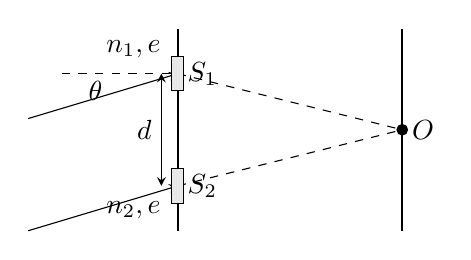
\begin{tikzpicture}[scale=0.95,>=stealth]
 \draw[thick] (0,-1.35) -- (0,1.35);
 \filldraw (0,0.75) circle (2pt) node[right] {\(S_1\)};
 \filldraw (0,-0.75) circle (2pt) node[right] {\(S_2\)};
 \draw[<->] (-0.22,-0.75) -- (-0.22,0.75) node[midway,left] {\(d\)};
 \draw[thick] (3.0,-1.35) -- (3.0,1.35);
 \filldraw (3.0,0) circle (2pt) node[right] {\(O\)};
 \draw[dashed] (0,0.75) -- (3.0,0);
 \draw[dashed] (0,-0.75) -- (3.0,0);
 \draw[->] (-2.0,0.15) -- (0,0.75);
 \draw[->] (-2.0,-1.35) -- (0,-0.75);
 \draw[dashed] (-1.55,0.75) -- (0,0.75);
 \node at (-1.1,0.52) {\(\theta\)};
 \draw[fill=gray!18] (-0.08,0.52) rectangle (0.08,0.98);
 \draw[fill=gray!18] (-0.08,-0.98) rectangle (0.08,-0.52);
 \node[left] at (-0.1,1.08) {\(n_1,e\)};
 \node[left] at (-0.1,-1.08) {\(n_2,e\)};
\end{tikzpicture}
\end{center}
\end{exercise}

\begin{solution}
中央 \(O\) 处的出射几何路程满足 \(S_1O=S_2O\)，所以相位差只来自两件事：斜入射时两缝处入射波本来就有相位差，以及两块介质片带来的附加光程差。

约定 \(\delta_{12}=L_1-L_2\)，即用通过 \(S_1\) 的光路减通过 \(S_2\) 的光路。介质片带来的光程差为 \(\delta_{\text{film}}=(n_1-n_2)e\)。
按原图的入射方向，波先到达上缝 \(S_1\)，后到达下缝 \(S_2\)。因此以 \(S_1\) 光路减 \(S_2\) 光路时，斜入射带来的入射端光程差为
 \(\delta_{\text{inc}}=-d\sin\theta,\qquad \delta_{12}=\delta_{\text{film}}+\delta_{\text{inc}} =(n_1-n_2)e-d\sin\theta,\qquad \Delta\phi_{12}=\frac{2\pi}{\lambda}\left[(n_1-n_2)e-d\sin\theta\right].\) 
总光程差和相位差就由上式给出。
若题目改成正入射，\(\theta=0\)，结果退化为两块介质片的相位差；若反过来定义“第二路减第一路”，整个相位差会整体变号，但明暗判据不变。
\end{solution}

\begin{theorem}[薄透镜的等光程性]
\begin{enumerate}
    \item 平行光经薄透镜后会汇聚到焦点。对称地看，凡是入射方向相同、出射到同一焦点的几条光线，薄透镜只改变它们的传播方向，不改变它们到焦点的总光程，所以它们在焦点处同相。
    \item 薄透镜可把近轴平行光汇聚于焦平面。因为透镜各部分对称，入射于透镜不同位置的平行光，经过透镜后到焦平面的总光程相等，故焦平面可看作等光程面。
    \item 物点 \(S\) 经薄透镜成像为 \(S'\) 时，从 \(S\) 出发、经透镜到 \(S'\) 的各条近轴光线，光程相等。
\end{enumerate}
\[
L_{AF}=L_{BF}=L_{CF}.
\]
\end{theorem}

\begin{exercise}[2011级期末：双缝装置浸入透明液体后的级次变化]
在杨氏双缝干涉实验中，设 \(SS_1=SS_2\)，用波长为 \(\lambda\) 的单色光照射双缝 \(S_1,S_2\)，通过空气后在屏 \(E\) 上形成干涉条纹。已知屏上某点 \(P\) 处为第三级明纹。若将整个装置放入某种透明液体中，\(P\) 点变为第四级明纹，求该液体的折射率 \(n\)。
\end{exercise}

\begin{solution}
整个装置浸入液体后，几何路程差 \(\Delta r\) 不变，改变的是光程差：同一段几何路程在液体中要乘上折射率 \(n\)。因此这题不是条纹间距简单缩放，而是同一个屏上点 \(P\) 对应的级次改变。空气中 \(P\) 为第三级明纹，说明 \(\Delta r=3\lambda\)。液体中光程差变为 \(\Delta L'=n\Delta r\)；若 \(P\) 变为第四级明纹，则
 \(n\Delta r=4\lambda,\qquad \Delta r=3\lambda \implies 3n\lambda=4\lambda \implies n=\frac43\approx 1.33.\) 
\end{solution}


\begin{exercise}[2007级期末：双缝明纹加高折射率反射面后变暗]
在双缝干涉实验中，屏幕 \(E\) 上 \(P\) 点原来是明条纹。若将缝 \(S_2\) 盖住，并在 \(S_1S_2\) 连线的垂直平分面处放一高折射率介质反射面 \(M\)，使 \(S_1\) 经反射面形成的虚像位置与原来的 \(S_2\) 等效。判断此时 \(P\) 点是明条纹还是暗条纹。

\begin{center}

\includegraphics[width=0.30\linewidth]{pdf-exercises/pdf2007-q07-lloyd-mirror.png}
\end{center}
\end{exercise}

\begin{solution}
反射面放在 \(S_1S_2\) 连线的垂直平分面处，反射光可看成来自 \(S_1\) 关于镜面的虚像，而这个虚像与原来的 \(S_2\) 等效。几何光程关系因此继承了原双缝中 \(S_1,S_2\) 到 \(P\) 的关系。

原来 \(P\) 为明纹，说明两缝到 \(P\) 的光程差满足 \(\Delta L=k\lambda\)。现在一路为 \(S_1\) 直达 \(P\)，另一路为 \(S_1\) 经高折射率反射面反射后到 \(P\)。由于反射等效虚源为 \(S_2\)，几何部分仍对应整数倍波长；但从空气侧在高折射率介质表面反射，会产生半波损失，相当于额外相差 \(\lambda/2\)。因此总光程差变为
 \(\Delta L'=k\lambda+\frac{\lambda}{2} =\left(k+\frac12\right)\lambda.\) 
所以 \(P\) 点变为暗条纹。本题不是说“盖住一个缝就没有干涉”；反射面提供了第二路相干光，真正改变明暗的是高折射率反射带来的半波损失。
\end{solution}

\section{薄膜干涉公式与附加光程差}

\begin{center}

\includegraphics[width=0.5\linewidth]{pdf-exercises/5.png}
\end{center}

\begin{theorem}[薄膜干涉公式]
\textbf{物理模型：}平行薄膜厚度为 \(d\)，折射率为 \(n_2\)，置于折射率分别为 \(n_1,n_3\) 的两种介质之间；入射光在上表面的入射角为 \(i\)，在膜内的折射角为 \(\gamma\)。对反射光，先看由几何路程和介质折算出的光程差，再看反射时是否有半波损失。两束参与反射干涉的主光线可记为 \(b_1,b_2\)
\begin{align*}
\delta_1&=n_2\frac{2d}{\cos\gamma}-n_1\left(2d\frac{\sin\gamma}{\cos\gamma}\sin i\right)=n_2\frac{2d}{\cos\gamma}-2dn_2\frac{\sin^2\gamma}{\cos\gamma}=2dn_2\cos\gamma=2dn_2\sqrt{1-\sin^2\gamma}.\\
&=2dn_2\sqrt{1-\left(\frac{n_1}{n_2}\sin i\right)^2}=2d\sqrt{n_2^2-n_1^2\sin^2 i}
\end{align*}
附加光程差 \(\delta_2\) 只由两次反射是否翻相决定：
\begin{itemize}
    \item 若 \(n_1<n_2<n_3\) 或 \(n_1>n_2>n_3\)，两束光在反射时经历的半波损失次数相同，\(\delta_2=0\)；
    \item 若 \(n_1<n_2>n_3\) 或 \(n_1>n_2<n_3\)，两束光中恰有一束发生半波损失，\(\delta_2=\lambda/2\)。
\end{itemize}
因此，反射光的总光程差为
\[
\delta=2d\sqrt{n_2^2-n_1^2\sin^2 i}+\delta_2.
\]
若题目问反射光的明暗条件，则当$\delta_2=0$时，亮纹$k$从$0$开始：
\[
\delta=k\lambda\quad(\text{亮纹}),\qquad
\delta=\left(k+\frac12\right)\lambda\quad(\text{暗纹}).
\]
若题目问透射光，则透射光与反射光刚好相反：反射光加强时，透射光减弱；反射光减弱时，透射光加强。\[|\delta_{\text{反射光}} - \delta_{\text{透射光}}| = \frac{\lambda}{2}\] 反射光程差与透射光程差相差 $\lambda/2$（或 $\pi$）。
\end{theorem}

\begin{exercise}[2008级期末：空气中透明薄膜反射加强的最小厚度]
一束波长为 \(\lambda\) 的单色光由空气垂直入射到折射率为 \(n\) 的透明薄膜上，透明薄膜放在空气中。要使反射光得到干涉加强，求薄膜的最小非零厚度。
\end{exercise}

\begin{solution}
结构是“空气--薄膜--空气”。上表面反射从低折射率到高折射率，有半波损失；下表面反射从高折射率到低折射率，没有半波损失。因此两束反射光之间有一次半波损失。正入射时几何光程差为 \(2nd\)。若把一次半波损失写成附加光程 \(\lambda/2\)，反射加强条件为
 \[2nd+\frac{\lambda}{2}=k\lambda,\qquad k=1 \implies d_{\min}=\frac{\lambda}{4n}.\] 
\end{solution}

\begin{definition}[增透膜与增反膜]
    “增透膜”目标是让\textbf{反射光尽量相消}，从而把更多光送进透射方向。若希望某一目标波长的反射尽量弱，就让反射光相消。例如：若某一薄膜用于目标波长 \(\lambda\) 的增透设计，且两束主要反射光的反射相位突变相同，求薄膜折射率为 \(n\) 时的最小非零厚度。要让反射方向相消，最小非零厚度满足 \(2nd=\frac{\lambda}{2}\implies d_{\min}=\frac{\lambda}{4n}.\) 
\end{definition}


\begin{exercise}[油膜上下观察时为什么会看到不同颜色]
一层折射率 \(n_1=1.20\) 的油膜浮在海水表面，海水折射率 \(n_2=1.30\)。若太阳在头顶正上方，某处油膜厚度 \(d=\SI{460}{nm}\)。问从空中向下看时呈什么颜色；若潜水员从水下向上看，又会看到什么主颜色。
\end{exercise}
\begin{solution}
先算
 \(2n_1d=2\times1.20\times460\,\si{nm}=1104\,\si{nm}.\) 
空气--油膜和油膜--海水两次反射都发生在低折射率到高折射率界面，两束反射光没有相对半波损失。从空中看反射增强时
 \(2n_1d=k\lambda \implies \lambda=\frac{1104}{k}\,\si{nm}.\) 
试可见光范围，最显著的可见解为
 \(k=2\Rightarrow \lambda=552\,\si{nm},\) 
对应绿光。

从水下看的是透射光，强弱与反射光互补。透射增强可写成
 \(2n_1d+\frac{\lambda}{2}=k\lambda \implies \lambda=\frac{1104}{k-\frac12}\,\si{nm}.\) 
试可见光范围得
 \(k=2\Rightarrow \lambda=736\,\si{nm},\qquad k=3\Rightarrow \lambda=441.6\,\si{nm}.\) 
其中主显著可见颜色可取红光。

所以从空中向下看主呈绿色，从水下向上看主呈红色。最容易错的是把上下观察都按反射题处理；先问眼睛接收到的是哪一路光，明暗条件才不会套反。
\end{solution}

\begin{definition}[等厚干涉]
当干涉条纹的形状取决于“薄膜上厚度相同的点的轨迹”时，得到的就是\textbf{等厚干涉}。
若入射角保持不变，则薄膜干涉中的光程差主要由厚度 \(d\) 决定。于是：
\begin{itemize}
 \item 厚度相同的点，光程差相同；
 \item 光程差相同的点，会落在同一条明纹或暗纹上。
\end{itemize}
这就是为什么“等厚线长成什么样，条纹就长成什么样”。若等厚线是直线，条纹就是直线；若等厚线是圆，条纹就是圆环。
\end{definition}

\begin{exercise}[圆形油膜条纹为什么会一圈圈向中心数]
在平面玻璃片上放一油滴并展开成圆形油膜。已知单色光波长 \(\lambda=\SI{600}{nm}\)，玻璃折射率 \(n_1=1.50\)，油膜折射率 \(n_2=1.20\)，油膜中心最高点厚度 \(h=8.0\times10^2\,\si{nm}\)。问：反射观察时条纹如何分布，可见明纹有几条，各明纹处膜厚各是多少；若油膜继续展开，条纹怎样变化？
\end{exercise}

\begin{solution}
由油膜厚度从中心向边缘单调减小可知，\textbf{相同厚度对应同心圆}，条纹自然是一圈圈的圆环。反射明纹条件为 \(2n_2d=k\lambda\)，所以明纹对应的膜厚为
 \(d_k=\frac{k\times 600}{2\times1.20}\,\si{nm}=250k\,\si{nm}.\) 
于是
\[
d_0=0,\quad d_1=\SI{250}{nm},\quad d_2=\SI{500}{nm},\quad d_3=\SI{750}{nm},\quad d_4=\SI{1000}{nm}.
\]
由于油膜中心最高厚度只有
 \(h=\SI{800}{nm},\) 
所以能实际出现的明纹厚度只能满足 \(d_k\le h\)。因此可见明纹共有
 \(k=0,1,2,3\) 
这 \(4\) 条。对应膜厚分别为
 \(0,\ \SI{250}{nm},\ \SI{500}{nm},\ \SI{750}{nm}.\) 
\end{solution}

\section{劈尖薄膜的干涉}

\begin{conclusion}[劈尖薄膜的干涉]
两块平板夹成很小夹角时，中间的空气层或透明薄层厚度沿某一方向近似线性变化，这种薄膜称为\textbf{劈尖}。设劈尖角为 \(\alpha\)，薄膜折射率为 \(n\)，入射单色光波长为 \(\lambda\)。从棱边起沿垂直棱边方向量距离 \(x\)，则
\[
d=x\sin\alpha\simeq x\alpha\qquad(\alpha\ll 1).
\]
厚度相同的点光程差相同，所以劈尖的等厚条纹是一组与棱边平行的明暗相间直条纹。

反射光中若两束相干光之间只有一次半波损失，则
\[
\delta=2nd+\frac{\lambda}{2}.
\]
明暗条件为
\[
\begin{cases}
2nd+\dfrac{\lambda}{2}=k\lambda, & \text{明纹},\quad k=1,2,3,\dots,\\[6pt]
2nd+\dfrac{\lambda}{2}=(2k+1)\dfrac{\lambda}{2}, & \text{暗纹},\quad k=0,1,2,\dots.
\end{cases}
\]
因此棱边处 \(d=0\) 为暗纹；第 \(k\) 级明纹和第 \(k\) 级暗纹对应的厚度分别为
\[
d_k^{(\text{明})}=\frac{2k-1}{4n}\lambda\quad(k=1,2,3,\dots),
\qquad
d_k^{(\text{暗})}=\frac{k}{2n}\lambda\quad(k=0,1,2,\dots).
\]
相邻两条明纹或相邻两条暗纹的厚度差相同：
\[
\Delta d=d_{k+1}-d_k=\frac{\lambda}{2n}.
\]
若相邻同类条纹在表面上的距离为 \(l\)，则
\[
l\sin\alpha=\Delta d=\frac{\lambda}{2n},
\qquad
l=\frac{\lambda}{2n\sin\alpha}\simeq \frac{\lambda}{2n\alpha}.
\]
波长一定时，劈尖角越大，条纹间距越小，条纹越密；劈尖角过大时，条纹会难以分辨。

若两次反射的半波损失数相同，则附加的半波损失相互抵消，光程差改为
\[
\delta=2nd.
\]
这时棱边 \(d=0\) 为明纹，暗纹条件为
\[
2nd=(2k+1)\frac{\lambda}{2}\qquad(k=0,1,2,\dots).
\]
例如薄膜折射率为 \(n_2\)，且 \(n_1<n_2<n_3\) 时，上、下表面的反射都发生半波损失。若从棱边 \(O\) 起向右数，第五条暗纹落在薄膜表面某处，则 \(k=4\)，于是
\[
2n_2d=\frac{9}{2}\lambda,
\qquad
d=\frac{9\lambda}{4n_2}
=4.5\,\frac{\lambda}{2n_2}.
\]

劈尖干涉常用于测量小厚度和小形变：
\begin{enumerate}
  \item \textbf{测镀膜厚度。} 将基板上的镀膜腐蚀成劈尖形，用单色光垂直照射。由条纹级次或相邻条纹的厚度差 \(\lambda/(2n)\)，即可反推出薄膜厚度。
  \item \textbf{测细丝直径。} 把金属丝夹在两块平玻璃之间形成空气劈尖。若棱边到金属丝的距离为 \(L\)，相邻同类条纹间距为 \(l\)，金属丝直径为 \(D\)，则
  \[
  \alpha\simeq \frac{D}{L},
  \qquad
  l=\frac{\lambda}{2n\alpha},
  \qquad
  D=L\alpha=\frac{L\lambda}{2nl}.
  \]
  对空气劈尖取 \(n\simeq1\)。若 \(\lambda=\SI{589.3}{nm}\)，\(L=\SI{28.880}{mm}\)，30 条明纹间距总长为 \(\SI{4.295}{mm}\)，则
  \[
  l=\frac{4.295}{29}\,\si{mm},
  \qquad
  D=\frac{28.880\times 589.3\times 10^{-6}}{2(4.295/29)}\,\si{mm}
  \approx \SI{5.74e-2}{mm}.
  \]
  \item \textbf{测微小厚度改变量。} 当 \(\alpha\) 不变时，整体增加薄膜厚度不会改变条纹间距，只会使条纹整体移动。对一次半波损失的反射劈尖，
  \[
  2nd_k+\frac{\lambda}{2}=k\lambda
  \quad\Longrightarrow\quad
  k=\frac{2n}{\lambda}d_k+\frac{1}{2}.
  \]
  若厚度增加 \(\lambda/(2n)\)，则 \(k\to k+1\)，即高一级条纹移到原来低一级条纹的位置，整个干涉图样向干涉级低的方向移动，也就是向棱边移动。若条纹平移距离为 \(A\)，则
  \[
  \frac{A}{l}=\frac{H}{\lambda/(2n)}
  \qquad\Longrightarrow\qquad
  H=\frac{\lambda A}{2nl}.
  \]
  若用条纹移动测热膨胀，长度由 \(l_0\) 变到 \(l\)，温度由 \(t_0\) 变到 \(t\)，且条纹移动 \(N\) 条，则
  \[
  \Delta l=l-l_0=N\frac{\lambda}{2},
  \qquad
  \beta=\frac{\Delta l}{l_0(t-t_0)}
  =\frac{N\lambda}{2l_0(t-t_0)}.
  \]
  \item \textbf{检查光学表面质量。} 将待检表面 \(B\) 与参考平面组成空气劈尖。若 \(B\) 平整，条纹应为平直等距条纹；若 \(B\) 有凹坑或凸起，局部厚度改变会使条纹弯曲。设相邻条纹间距为 \(b\)，局部条纹偏移为 \(a\)，缺陷高度为 \(H\)，则
  \[
  \frac{a}{b}=\frac{H}{\lambda/2}
  \qquad\Longrightarrow\qquad
  H=\frac{\lambda}{2}\frac{a}{b}
  \]
  对空气劈尖成立；一般介质中把 \(\lambda/2\) 改为 \(\lambda/(2n)\)。
\end{enumerate}
\end{conclusion}

\begin{exercise}[2014级期末：滚柱间距变小时劈尖条纹数和间距怎样变]
两根直径有微小差别、彼此平行的滚柱之间距离为 \(L\)，其上放两块平板玻璃，中间形成空气劈尖。单色光垂直入射时产生等厚干涉条纹。若滚柱之间的距离 \(L\) 变小，判断在两滚柱之间观察到的条纹数和条纹间距怎样变化。
\end{exercise}

\begin{solution}
两滚柱直径差给定，所以两端的空气膜厚度差 \(\Delta d\) 不变；改变 \(L\) 只是改变劈尖角。

劈尖角小量近似为 \(\alpha\approx\Delta d/L\)。相邻同类条纹间距和两滚柱之间的总条纹数分别为
 \(\Delta x=\frac{\lambda}{2\alpha} =\frac{\lambda L}{2\Delta d},\qquad N\approx\frac{\Delta d}{\lambda/2} =\frac{2\Delta d}{\lambda}.\) 
当 \(L\) 变小时，\(\Delta d\) 不变，所以条纹数 \(N\) 不变，而条纹间距 \(\Delta x\) 变小。条纹数看总厚度差，条纹间距看厚度随位置变化的斜率；把两者混在一起，就会误以为间距变小必然让条纹数增加。
\end{solution}

\begin{exercise}[2006级期末：空气劈形膜上玻璃平移时条纹怎样动]
两块平玻璃构成空气劈形膜，左边为棱边，用单色平行光垂直入射。若上面的平玻璃慢慢地向上平移，判断干涉条纹的移动方向和条纹间隔变化。
\end{exercise}

\begin{solution}
劈尖条纹是等厚线。上玻璃若整体向上平移，劈尖角不变，因此厚度随位置的斜率不变；但每个位置的空气膜厚度都会增加同一个常量。

设平移前空气膜厚度近似为 \(d(x)=\alpha x\)，上板整体上移 \(h\) 后变为 \(d'(x)=h+\alpha x\)。某一条同级条纹要求膜厚等于固定值 \(d_k\)，因此新旧位置满足
 \(h+\alpha x'=d_k,\qquad \alpha x=d_k \implies x'=x-\frac{h}{\alpha}.\) 
所以条纹向棱边方向平移，条纹间隔不变。条纹间隔由斜率 \(\alpha\) 决定；平移只给厚度加常量，不改斜率，不能把“厚度增加”误判成“劈尖角变大”。
\end{solution}


\begin{exercise}[2008级期末：空气劈尖第四条明纹随劈尖角改变的位移]
用波长为 \(\lambda\) 的单色光垂直照射由两块平玻璃板构成的空气劈形膜，已知劈尖角为 \(\theta\)。若劈尖角变为 \(\theta'\)，求从劈棱数起的第四条明条纹位移值 \(\Delta x\)。
\end{exercise}

\begin{solution}
空气劈尖在反射光中有一次半波损失。距离劈棱 \(x\) 处膜厚近似为 \(d=x\theta\)，反射明纹满足总光程差为整数倍波长。

从劈棱起数，棱边处为暗纹，第四条明纹对应
 \(2x_4\theta+\frac{\lambda}{2}=4\lambda.\) 
于是
 \(x_4=\frac{7\lambda}{4\theta},\qquad x_4'=\frac{7\lambda}{4\theta'}.\) 
位移按新位置减旧位置记：
 \(\Delta x=x_4'-x_4 =\frac{7\lambda}{4}\left(\frac{1}{\theta'}-\frac{1}{\theta}\right) =\frac{7\lambda(\theta-\theta')}{4\theta\theta'}.\) 
第四条明纹离棱边不是 \(4\) 个条纹间距，而是 \(3.5\) 个条纹间距，因为反射光在棱边处为暗纹。若 \(\theta'\) 变小，条纹间距变大，第四明纹应向远离棱边方向移动，公式也给出正位移。
\end{solution}


\begin{exercise}[用劈尖条纹间距测金属细丝直径时为什么先写几何斜率]
把金属细丝夹在两块平玻璃之间形成空气劈尖。用波长 \(\lambda=\SI{589.3}{nm}\) 的单色光垂直照射，已知金属丝到劈尖顶点的距离 \(L=\SI{28.880}{mm}\)，测得 \(30\) 条明纹跨越的总长度为 \(\SI{4.295}{mm}\)。求金属细丝直径 \(D\)。
\end{exercise}

\begin{solution}
这类题看上去在测长度，其实真正要写的是“厚度沿长度方向怎样线性增长”。也就是说，先把劈尖的几何斜率写成 \(\alpha\approx D/L\)，再用条纹间距把 \(\alpha\) 反推出去。

这里空气劈尖取 \(n=1\)，且 \(30\) 条明纹跨越的是 \(29\) 个条纹间距，所以
\[
l=\frac{4.295}{29}\,\si{mm}\approx \SI{0.1481}{mm},\qquad
D=L\alpha=L\frac{\lambda}{2l}
=\frac{28.880\times 589.3\times10^{-6}}{2\times0.1481}\,\si{mm}
\approx \SI{0.0574}{mm}.
\]
细丝直径约为 \(\SI{5.74e-2}{mm}=\SI{57.4}{\micro m}\)，落在几十微米量级是合理的。这里不能把 \(30\) 条条纹误当成 \(30\) 个间距，也不能漏掉空气层对应 \(n=1\)。
\end{solution}


\begin{exercise}[空气劈尖条纹弯向厚端时怎样判断凸凹缺陷]
光学平板玻璃 \(A\) 与待测工件 \(B\) 间形成空气劈尖，左侧为空气膜薄端、右侧为空气膜厚端。用波长 \(\lambda=\SI{500}{nm}\) 的单色光垂直照射，反射光干涉条纹中弯曲部分向厚端偏移，且顶点恰好与其右边相邻直条纹的连线相切。判断工件上表面缺陷是凸起还是凹槽，并求最大高度或深度。
\end{exercise}

\begin{solution}
题目说弯曲顶点恰好与右边相邻直条纹相切，表示缺陷导致的最大膜厚变化正好相当于相邻一级条纹，即
 \(h_{\max}=\frac{\lambda}{2} =\frac{\SI{500}{nm}}{2} =\SI{250}{nm}.\) 
所以缺陷为凸起，最大高度为 \(\SI{250}{nm}\)。
\end{solution}

\section{牛顿环}

\begin{conclusion}[牛顿环]
\textbf{牛顿环}由一块平板玻璃和一枚曲率半径 \(R\) 很大的平凸透镜组成。两者之间形成一层厚度随半径变化的空气膜，相同厚度对应同一光程差，所以图样是同心圆环。

设距接触点半径为 \(r\) 处膜厚为 \(d\)。由几何关系
\[
r^2=R^2-(R-d)^2=2dR-d^2\approx 2dR\qquad(R\gg d),
\]
得
\[
d\approx \frac{r^2}{2R}.
\]
在反射光中，空气膜上下表面反射光之间有一次半波损失，因此
\[
\delta=2d+\frac{\lambda}{2}.
\]
于是反射暗环、明环分别满足
\[
\begin{cases}
2d=k\lambda, & \text{暗环},\quad k=0,1,2,\dots,\\[4pt]
2d=(2k-1)\dfrac{\lambda}{2}, & \text{明环},\quad k=1,2,3,\dots.
\end{cases}
\]
代入 \(d\approx r^2/(2R)\) 得
\[
r_k=\sqrt{kR\lambda}\quad(\text{暗环},\,k=0,1,2,\dots),\qquad
r_k=\sqrt{\frac{(2k-1)R\lambda}{2}}\quad(\text{明环},\,k=1,2,3,\dots).
\]
从反射光看，中心是暗点；从透射光看，中心是亮点。

又有
\[
r_k^2=R\left(k-\frac12\right)\lambda,\qquad
r_{k+1}^2-r_k^2=R\lambda,\qquad
r_{k+1}-r_k=\frac{R\lambda}{r_{k+1}+r_k},
\]
所以环纹间距随 \(r\) 增大而减小，图样呈现“中间疏，边缘密”。

牛顿环常见于以下几类问题：
\begin{enumerate}
  \item \textbf{检查平凸透镜曲率半径是否合格。} 受检元件与标准平板嵌合良好时，没有牛顿环，说明合格；若 \(R<R_0\)，加压时条纹向边缘移动；若 \(R>R_0\)，加压时条纹向中心移动。
  \item \textbf{测量透镜曲率半径。} 若测得第 \(k\) 个暗环半径为 \(r_k\)，第 \(k+m\) 个暗环半径为 \(r_{k+m}\)，则
  \[
  R=\frac{r_{k+m}^2-r_k^2}{m\lambda}.
  \]
  例如 \(\lambda=\SI{633}{nm}\)，\(r_k=\SI{5.63}{mm}\)，\(r_{k+5}=\SI{7.96}{mm}\)，得 \(R\approx\SI{10.0}{m}\)。
  \item \textbf{观察圆形油膜的干涉。} 若平面玻璃片上有一层圆形油膜，并从反射光中观察同心圆条纹，则仍可用牛顿环思路处理。以 \(\lambda=\SI{600}{nm}\)、\(n_1=1.50\)、\(n_2=1.20\) 为例，反射中的两次半波损失相互抵消，故
  \[
  \delta=2n_2d_k,\qquad d_k=k\frac{\lambda}{2n_2}=k\times\SI{250}{nm}\quad(k=0,1,2,\dots).
  \]
  因而油膜边缘 \(d_0=0\) 为明纹；当中心最高点与玻璃片上表面的距离 \(h=\SI{8.0e2}{nm}\) 时，可见 \(k=0,1,2,3\) 四条明纹。油膜展开时厚度减小，条纹数减少，条纹间距变大。
\end{enumerate}
\end{conclusion}




\begin{exercise}[牛顿环测曲率半径]
在牛顿环实验中，已知单色光波长为 \(\lambda\)，测得第 \(k\) 个暗环半径为 \(r_k\)，第 \(k+m\) 个暗环半径为 \(r_{k+m}\)。求平凸透镜的曲率半径 \(R\)。
\end{exercise}

\begin{solution}
题目给的是两个\textbf{暗环半径}，目标是求曲率半径 \(R\)。由反射暗环关系分别写出两级半径，再相减消去未知级次 \(k\)，于是
\[
\begin{aligned}
r_k^2&=kR\lambda,\qquad r_{k+m}^2=(k+m)R\lambda,\\
r_{k+m}^2-r_k^2&=(k+m)R\lambda-kR\lambda=mR\lambda
\implies
R=\frac{r_{k+m}^2-r_k^2}{m\lambda}.
\end{aligned}
\]
\(r^2/\lambda\) 的量纲是长度，和 \(R\) 一致。用平方差而不用半径直接相减的好处，是不必纠缠中心究竟记作第零级还是第一级；只要两条都是暗环，同一条公式就成立。
\end{solution}

\begin{exercise}[空气换成液体后牛顿环半径怎样反推折射率]
平凸透镜顶点和平板玻璃接触，用单色光垂直照射，观察反射光形成的牛顿环。测得中央暗斑外第 \(k\) 个暗环在空气中半径为 \(r_1\)。若将透镜和玻璃板之间的空气换成某种液体，且液体折射率小于玻璃折射率，第 \(k\) 个暗环半径变为 \(r_2\)。求该液体折射率。
\end{exercise}

\begin{solution}
同一个第 \(k\) 个暗环，对应的是同一级干涉条件；换液体后改变的是薄膜折射率，几何关系 \(d\approx r^2/(2R)\) 不变。

反射暗环条件可写成 \(2nd=k\lambda\)，又有 \(d=r^2/(2R)\)。空气中 \(n\approx1\)，所以
 \(2\cdot 1\cdot \frac{r_1^2}{2R}=k\lambda \implies r_1^2=kR\lambda.\) 
换成液体后，
 \(2n\frac{r_2^2}{2R}=k\lambda \implies nr_2^2=kR\lambda.\) 
两式相除得
 \(n=\frac{r_1^2}{r_2^2}.\) 
液体折射率 \(n>1\) 时，同一级暗环需要更小几何厚度，因此 \(r_2<r_1\)，于是 \(r_1^2/r_2^2>1\)，方向合理。牛顿环公式天然是半径平方关系，不能直接拿半径比来代替平方比。
\end{solution}

\begin{exercise}[2011级期末：浸入液体的牛顿环中心暗斑]
平凸透镜与平板玻璃构成牛顿环装置，整个装置浸入折射率为 \(n=\num{1.60}\) 的液体中。平凸透镜折射率为 \(\num{1.68}\)，平板玻璃折射率为 \(\num{1.58}\)。凸透镜可沿轴线 \(OO'\) 上下移动，用波长 \(\lambda=\SI{500}{nm}\) 的单色光垂直入射，从上方观察反射光。若调节后看到中心为暗斑，求凸透镜顶点到平板玻璃的最小距离。

\begin{center}
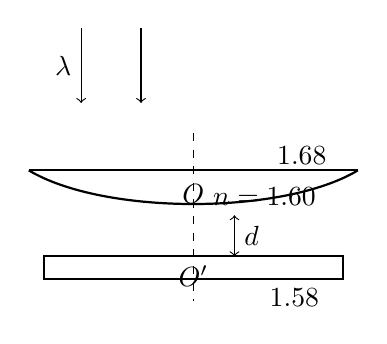
\begin{tikzpicture}[scale=0.95]
 \draw[->] (-1.5,2.6) -- (-1.5,1.6) node[midway,left] {\(\lambda\)};
 \draw[->] (-0.7,2.6) -- (-0.7,1.6);
 \draw[thick] (-2.2,0.7) .. controls (-1.2,0.1) and (1.2,0.1) .. (2.2,0.7);
 \draw[thick] (-2.2,0.7) -- (2.2,0.7);
 \draw[thick] (-2.0,-0.45) rectangle (2.0,-0.75);
 \draw[dashed] (0,1.2) -- (0,-1.05);
 \draw[<->] (0.55,0.10) -- (0.55,-0.45) node[midway,right] {\(d\)};
 \node at (0.95,0.35) {\(n=1.60\)};
 \node at (1.45,0.9) {\(1.68\)};
 \node at (1.35,-1.0) {\(1.58\)};
 \node[above] at (0,0.12) {\(O\)};
 \node[below] at (0,-0.45) {\(O'\)};
\end{tikzpicture}
\end{center}
\end{exercise}

\begin{solution}
液体膜内往返光程差需满足
 \(2nd=\left(k+\frac12\right)\lambda,\qquad k=0,1,2,\dots\) 
求最小距离，取 \(k=0\)，得
 \(d_{\min}=\frac{\lambda}{4n} =\frac{\SI{500}{nm}}{4\times1.60} =\SI{78.125}{nm}.\) 
因此最小距离约为 \(\SI{78.1}{nm}\)。如果中心两面相接 \(d=0\)，因为两次反射都没有相对半波损失，中心应为亮而不是暗；只凭“牛顿环中心常暗”直接选 \(0\)，就忽略了三种介质的折射率顺序。
\end{solution}


\begin{exercise}[两种波长第五个牛顿环明环对应膜厚差]
平凸透镜凸面朝下放在平玻璃板上，透镜刚好与玻璃板接触。波长分别为 \(\lambda_1=\SI{600}{nm}\)、\(\lambda_2=\SI{500}{nm}\) 的两种单色光垂直入射，观察反射光形成的牛顿环。求从中心向外数的两种光的第五个明环所对应的空气膜厚度之差。
\end{exercise}

\begin{solution}
反射牛顿环中心为暗，明环条件要带半级差。题目问的是膜厚差，不需要再把膜厚换成半径。

反射明环满足
 \(2d=\left(k-\frac12\right)\lambda,\qquad k=1,2,3,\dots\) 
第五个明环对应 \(k=5\)，故
 \(d=\frac{k-\frac12}{2}\lambda =\frac{9}{4}\lambda,\qquad \Delta d=\frac94(\lambda_1-\lambda_2) =\frac94(600-500)\,\si{nm} =\SI{225}{nm}.\) 
第五个明环不是 \(2d=5\lambda\)，而是 \(2d=(5-\frac12)\lambda\)。中心暗点会把明环条件整体错开半级。
\end{solution}

\begin{exercise}[2005级期末：迈克耳孙干涉仪中插入薄膜的厚度]
在迈克耳孙干涉仪的一支光路中，放入一片折射率为 \(n\) 的透明介质薄膜后，测出两束光的光程差改变量为一个波长 \(\lambda\)。求薄膜厚度。
\end{exercise}

\begin{solution}
迈克耳孙干涉仪中一支光路要往返一次。插入薄膜后，空气段被介质段替代，单程附加光程为 \((n-1)d\)，往返后要乘 \(2\)。

题目给出光程差改变量为一个波长满足
 \(2(n-1)d=\lambda \implies d=\frac{\lambda}{2(n-1)}.\) 
最容易漏掉的是迈克耳孙装置的往返程，把附加光程误写成 \((n-1)d\)。这里的 \(n-1\) 也说明我们比较的是“介质替代空气”带来的附加光程，而不是单纯的 \(nd\)。
\end{solution}

\begin{exercise}[2005级期末：牛顿环透镜上移时移过固定点的条纹数]
用波长为 \(\lambda\) 的单色光垂直照射牛顿环装置，观察从空气膜上下表面反射的光形成的牛顿环。若使平凸透镜从顶点与平面玻璃接触开始，慢慢垂直向上移动到两者距离为 \(d\)，求移过视场中某固定观察点的条纹数目。
\end{exercise}

\begin{solution}
固定观察点处的条纹变化，本质上是该点空气膜厚度随透镜整体上移而增加。反射牛顿环中，相邻同类条纹对应的膜厚变化为 \(\lambda/2\)。
透镜整体上移 \(d\) 后，固定观察点处空气膜厚度增加 \(d\)，所以两束反射光的几何光程差增加 \(\Delta L=2d\)。每改变一个波长，就有一条同类条纹移过固定点，因此 \(N=2d/\lambda\)。
\end{solution}


\chapter{光的衍射}

\section{衍射现象，惠更斯-菲涅尔原理}

\begin{conclusion}[衍射现象与惠更斯-菲涅尔原理]
当光在传播中遇到障碍物或孔缝时，除了沿直线前进，还会绕过障碍物边缘进入几何阴影区，这种偏离直线传播的现象叫\textbf{衍射}。
常见的衍射图样有两类：圆孔衍射常呈\textbf{同心圆环}，单缝衍射常呈\textbf{明暗相间的条纹}。它们本质上都是波前被限制后，各部分子波相干叠加的结果。
\begin{itemize}
  \item 光的衍射图样沿着受限方向扩展。
  \item 光受限越厉害，衍射图样越展开，衍射效应越强。
\end{itemize}
惠更斯-菲涅尔原理指出：波前上每个面元 \(dS\) 都可看成一个次波源，观察点 \(P\) 处的振动，是波前 \(S\) 上各子波在该点产生振动的相干叠加，因此
\[
E(P)=\int_S \frac{C K(\theta)}{r}\cos\!\left(\omega t-\frac{2\pi r}{\lambda}\right)\mathrm dS .
\]
其中，\(S\) 表示 \(t\) 时刻的波前，\(dS\) 表示波阵面上面元（子波波源），\(r\) 为该面元到 \(P\) 点的距离，\(K(\theta)\) 为倾斜因子。按光源、孔缝与屏的相对距离，衍射可分为两类：\textbf{菲涅耳衍射}是光源、屏与缝相距有限远；\textbf{夫琅禾费衍射}是光源、屏与缝相距无限远。实际实验中常借助透镜把平行光照明和焦平面观察结合起来，从而实现夫琅禾费衍射。
\end{conclusion}

\begin{figure}[htbp]
\centering

\includegraphics[width=0.6\textwidth]{pdf-exercises/7.png}
\caption{菲涅尔衍射和夫琅禾费衍射的示意图}
\end{figure}

\section{菲涅耳半波带与半波带法}

\begin{definition}[菲涅耳半波带]
\textbf{惠更斯原理}说，狭缝 \(AB\) 处波阵面上的每一点都可以看成新的波源，向各个方向发射子波。对观察点 \(P\) 而言，把波阵面上到 \(P\) 的光程差按 \(\lambda/2\) 逐段划分，得到的一段一段区域就叫\textbf{菲涅耳半波带}。相邻半波带到 \(P\) 的相位差为 \(\pi\)，因此最容易成对抵消。

对单缝衍射而言，衍射角 \(\theta\) 是衍射光与狭缝法线之间的夹角；屏上某点的光强，就是狭缝波阵面上所有具有相同衍射角的子波在该点的相干叠加。不同的 \(\theta\) 或不同的观察点 \(P\)，对应的光程差不同，叠加强度也不同。狭缝上下边缘 \(A,B\) 之间的最大光程差为
\[
\delta=BC=a\sin\theta.
\]
当 \(\theta=0\) 时，\(\delta=0\)，中心 \(O\) 为明纹（主极大）。
\end{definition}

\begin{figure}[htbp]
\centering

\includegraphics[width=0.6\textwidth]{pdf-exercises/9.png}
\caption{半波带法示意图}
\end{figure}

\begin{definition}[半波带法]
缝上下边缘到 \(Q\) 的最大光程差：$\delta=a\sin\theta$
\begin{itemize}
\item 中央明纹中心
\[
a\sin\theta=0
\]所有子波到屏上中心点的光程差都为 \(0\)，同相叠加，所以是中央明纹中心，也是主极大。
\item 暗纹
\[
a\sin\theta=\pm 2k\frac{\lambda}{2}=\pm k\lambda
\]这时单缝可分成 \(2k\) 个半波带。相邻半波带两两抵消，光强为零，形成暗纹。
\item 次级明纹
\[
a\sin\theta=\pm(2k+1)\frac{\lambda}{2}
\]这时单缝可分成 \(2k+1\) 个半波带。前 \(2k\) 个成对抵消，剩下一个半波带，所以形成明纹。但它不是主极大，亮度比中央明纹弱很多。
\item 介于明暗之间
\[
a\sin\theta\neq k\frac{\lambda}{2}
\]这时不能刚好分成整数个半波带，抵消不完全，也不是严格的明纹中心，所以光强介于明暗之间。
\end{itemize}
\[
\boxed{
\begin{array}{c|c}
a\sin\theta=0 & \text{中央明纹中心}\\
a\sin\theta=\pm k\lambda & \text{暗纹}\\
a\sin\theta=\pm(2k+1)\lambda/2 & \text{次级明纹}\\
\text{其他} & \text{明暗之间}
\end{array}}
\]这里 \(k=1,2,3,\dots\)。注意中央明纹不能简单归入“奇数个半波带”，因为它对应的是光程差为零，不是分出一个半波带。
\end{definition}

\section{单缝的夫琅禾费衍射}

\begin{figure}[htbp]
\centering

\includegraphics[width=0.6\textwidth]{pdf-exercises/8.png}
\caption{单缝的夫琅禾费衍射示意图}
\end{figure}

\begin{theorem}[单缝衍射的光强分布]
设单缝宽度为 \(a\)，缝上每个微小面元都发出同频同相的次级波。观察方向与中央方向夹角为 \(\theta\)。缝上相距 \(y\) 的两点，到观察方向的光程差约为$y\sin\theta$，对应相位差为
\[
\varphi=\frac{2\pi}{\lambda}y\sin\theta
\]
所以来自宽度元 \(dy\) 的振动可以写成
\[
dE=C e^{i\frac{2\pi}{\lambda}y\sin\theta}\,dy
\]总振幅就是把整个单缝从 \(-a/2\) 到 \(a/2\) 积分：
\[
E_\theta=C\int_{-a/2}^{a/2}e^{i\frac{2\pi}{\lambda}y\sin\theta}\mathrm dy=C\frac{2\sin\left(\frac{\pi a\sin\theta}{\lambda}\right)}
{\frac{2\pi\sin\theta}{\lambda}}
\]令$\alpha=\frac{\pi a\sin\theta}{\lambda}$（总相位差的一半，整个缝宽对应的总相位差是$\Delta\varphi=\frac{2\pi}{\lambda}a\sin\theta=2\alpha$）就得到$E_\theta=Ca\frac{\sin\alpha}{\alpha}$，中央方向 \(\theta=0\) 时，全缝同相叠加，振幅为$E_0=Ca$，所以由光强正比于振幅平方：
\[
\frac{E_\theta}{E_0}=\frac{\sin\alpha}{\alpha}\implies
I_\theta=I_0\left(\frac{\sin\alpha}{\alpha}\right)^2
\]当 \(\theta=0\) 时，单缝上所有点到屏幕中心 \(O\) 的光程都相同。此时$a\sin\theta=0$，所有子波同相叠加，所以中心处光强最大。这就是中央明纹中心，也叫主极大，亮度\(I_P=I_0\)。
\end{theorem} 

\begin{theorem}[第 \(k\) 级明纹的光强]
对于第 \(k\) 级明纹，对该处光强的贡献只有 \(AB\) 波阵面平行光的 \(1/(2k+1)\)。事实上，当某个方向对应
\[
a\sin\theta=\pm(2k+1)\frac{\lambda}{2}
\]时，整个单缝可以被分成 \(2k+1\) 个半波带。前 \(2k\) 个半波带两两抵消；最后剩下 1 个半波带没有配对；所以这个方向仍然是明纹，但只剩一小部分贡献。因此级数越高，半波带数越多，能留下来的有效贡献越小，明纹就越暗。
\end{theorem}

\begin{figure}[htbp]
\centering

\includegraphics[width=0.6\textwidth]{pdf-exercises/10.png}
\caption{明暗纹位置与宽度辅助图}
\end{figure}

\begin{theorem}[暗纹的位置与宽度，中央明纹的半角/半线宽度，中央明纹宽度]
第 \(k\) 级暗纹
\[a\sin\theta\approx a\theta_k=k\lambda\implies \theta_k=\frac{k\lambda}{a},~k=1,2,3...\]第一级暗纹对应$\theta_1=\frac{\lambda}{a}$，中央明纹的半角宽度：$\theta_1=\frac{\lambda}{a}$，又
\[
x_k=f\tan\theta_k=f\sin\theta_k=f\frac{k\lambda}{a}
\]也就是说：级次越高，离中心越远；波长越长，条纹越散；焦距越大，屏上图样越放大；缝宽越小，衍射越明显，条纹越分散。中央明纹中心到第一级暗纹的距离设为 \(x_1\)，则$x_1=f\theta_1=f\sin\theta_1=f\frac{\lambda}{a}$就是中央明纹的半线宽度。中央明纹总宽度是左右两个 \(x_1\)：
\[
\Delta x_0=2x_1=2f\frac{\lambda}{a}
\]告诉我们中央明纹宽度与缝宽成反比，缝越窄，中央明纹越宽。除了中央明纹外，其它明纹宽度是中央明纹宽度的一半。相邻两个暗纹之间的距离为
\[
\Delta x=x_{k+1}-x_k=\frac{(k+1)\lambda f}{a}-\frac{k\lambda f}{a}=\frac{\lambda f}{a}=\frac12\Delta x_0.
\]缝宽 \(a\) 变小；
第一级暗纹角度 \(\theta_1\) 变大；
中央明纹宽度 \(\Delta x_0\) 变大；
整个衍射图样展开得更明显。
\end{theorem}

\begin{theorem}[单缝衍射的动态变化]
\begin{enumerate}
\item 单缝上下移动：衍射图不变。如果只把单缝 \(R\) 上下移动，而透镜 \(L\) 和观察屏 \(P\) 不动，那么屏上的衍射图样不发生平移，中央明纹仍然在透镜光轴上。单缝上移，零级明纹仍在透镜光轴上。（单缝位置变了；但透镜仍把同一衍射角 \(\theta\) 的平行光汇聚到焦平面上的同一位置；所以衍射角分布没有变；屏上强度分布也不变。）第 \(k\) 级暗纹与中心的距离仍为
\[
x_k=\theta_k f=\frac{k\lambda}{a}f.
\]只要缝宽 \(a\)、波长 \(\lambda\)、焦距 \(f\) 不变，这个距离就不变。
\item 如果透镜向上移动，它的光轴也向上移动，那么零级明纹跟着光轴移动；整个衍射图样一起平移；但各级暗纹相对中心的距离不变。也就是说，透镜移动改变的是图样在屏上的整体位置，不改变图样内部结构。所以仍有
\[
x_k=\frac{k\lambda f}{a}.
\]这里的 \(x_k\) 是相对于新的中心位置测量的。
\end{enumerate}    
\end{theorem}


\begin{exercise}[单缝衍射：由明纹位置判断级次]
在单缝夫琅禾费衍射实验中，单缝宽度 \(a=\SI{0.10}{mm}\)，透镜焦距 \(f=\SI{100}{mm}\)，入射光波长 \(\lambda=\SI{500}{nm}\)。屏上距中央明纹中心 \(x=\SI{1.75}{mm}\) 的 \(P\) 点为明纹。设衍射角很小，求：
\begin{enumerate}
\item \(P\) 点的明纹级次；
\item 对应于 \(P\) 点，单缝可分成多少个半波带；
\item 若缝宽增加一倍而 \(P\) 点位置不变，\(P\) 点变成什么条纹。
\end{enumerate}
\end{exercise}

\begin{solution}
小角近似下，
\[
\sin\theta\approx\tan\theta=\frac{x}{f}.
\]
先把 \(P\) 点对应的最大光程差写成波长的倍数：
\[
\frac{a\sin\theta}{\lambda}\approx\frac{ax}{f\lambda}
=\frac{0.10\times1.75}{100\times 5.00\times10^{-4}}=3.5,
\]
其中 \(\lambda=\SI{500}{nm}=5.00\times10^{-4}\,\si{mm}\)。单缝明纹近似条件为
\[
a\sin\theta=(2k+1)\frac{\lambda}{2}\implies\frac{2k+1}{2}=3.5\implies k=3.
\]
所以 \(P\) 点是第 \(3\) 级明纹。此时$a\sin\theta=\frac{7\lambda}{2}$，每个半波带对应光程差 \(\lambda/2\)，故单缝可分成 \(7\) 个半波带。若缝宽增加一倍，观察点 \(P\) 不动，则 \(\theta\) 不变，而
\[
a'\sin\theta=2a\sin\theta=7\lambda.
\]
这满足单缝暗纹条件 \(a'\sin\theta=K\lambda\)，且 \(K=7\)，所以 \(P\) 点变为第 \(7\) 级暗纹。
\end{solution}


\begin{exercise}[2008级期末：由钠黄光中央明纹宽度推蓝紫光宽度]
在单缝夫琅禾费衍射实验中，设第一级暗纹的衍射角很小。若钠黄光 \(\lambda_1\approx\SI{589}{nm}\) 的中央明纹宽度为 \(\SI{4.0}{mm}\)，求 \(\lambda_2=\SI{442}{nm}\) 的蓝紫色光的中央明纹宽度。
\end{exercise}

\begin{solution}
同一装置中，单缝宽度 \(a\) 和透镜焦距 \(f\) 不变，中央明纹宽度只随波长成正比：
 \(\Delta x_0=\frac{2f\lambda}{a} \implies \frac{\Delta x_2}{\Delta x_1}=\frac{\lambda_2}{\lambda_1},\qquad \Delta x_2 =4.0\,\si{mm}\times\frac{442}{589} \approx \SI{3.0}{mm}.\) 
蓝紫光波长比钠黄光短，算出的中央明纹也更窄，这和衍射图样随波长缩小的判断一致。
\end{solution}

\begin{exercise}[2012级期末：由两侧第三级暗纹距离反推单缝波长]
平行单色光垂直入射到缝宽 \(a=\SI{0.15}{mm}\) 的单缝上。缝后有焦距 \(f=\SI{400}{mm}\) 的凸透镜，在其焦平面上放置观察屏。若屏幕中央明纹两侧的两个第三级暗纹之间的距离为 \(\SI{8}{mm}\)，设衍射角很小，求入射光波长。
\end{exercise}
\begin{solution}
 \[a\sin\theta_k=k\lambda,\qquad x_k\approx f\tan\theta_k\approx f\sin\theta_k\approx\frac{kf\lambda}{a}\] 
题目给的是两侧第三级暗纹之间的全距离，故单侧 \(x_3=\SI{4}{mm}\)，于是
 \[\lambda=\frac{a x_3}{3f} =\frac{0.15\,\si{mm}\times 4\,\si{mm}}{3\times 400\,\si{mm}} =5.0\times10^{-4}\,\si{mm} =\SI{500}{nm}\]
\end{solution}

\section{圆孔夫琅禾费衍射与光学仪器的分辨本领}

\begin{figure}[htbp]
\centering

\includegraphics[width=0.6\textwidth]{pdf-exercises/11.png}
\caption{圆孔衍射示意图}
\end{figure}

\begin{definition}[圆孔夫琅禾费衍射]
光通过圆孔以后会形成一个有大小的亮斑，也就是艾里斑。图中$d$为艾里斑直径，$\theta$为衍射角，$\theta_1$为艾里斑的半角宽度，也就是从光轴到第一暗环边界的角度
\[\theta_1=\frac{d/2}{f}=1.22\frac{\lambda}{D}\]
屏上中央亮斑的半径是 \(d/2\)，放到透镜焦平面里去看，它对应的角宽就是 \(\theta_1\)。而这个角宽又由波长 \(\lambda\) 和孔径 \(D\) 决定。孔越大，\(\theta_1\) 越小，斑越小；波长越长，\(\theta_1\) 越大，斑越大。
\end{definition}

\begin{definition}[光学仪器能否区分两个物点与瑞利判据]
真实的光是波，物点 \(S\) 成像后是一个有扩展范围的衍射斑；如果还有另一个物点 \(S_1\)，它也会形成另一个艾里斑；两个物点如果都在透镜的焦平面上，那么屏上看到的是两个艾里斑的叠加；由于这两个点光源是不相干的，所以总光强是  \[
I=I_1+I_2
\]对于两个强度相等的不相干点光源（物点），如果一个点光源的衍射图样的主极大，刚好和另一个点光源衍射图样的第一极小重合，那么这两个点光源（或物点）就恰好能被这一光学仪器分辨。（两个亮斑只要“肩碰肩”，中间还能看出一点凹下去，就算刚好分辨；如果凹不出来，就分不清了。）在瑞利条件下，两个物点刚好能分辨时，它们对仪器中心的张角，就是最小分辨角：
\[
\delta\theta_0=1.22\frac{\lambda}{D}
\]
这其实就是圆孔衍射的第一暗环半角宽度。也就是说第一暗环半角宽度，最小分辨角本质上是同一个量。接着定义分辨率（分辨本领）：
\[
R=\frac{1}{\delta\theta_0}=\frac{D}{1.22\lambda}\propto D,\ \frac{1}{\lambda}
\]孔径 \(D\) 越大，分辨本领越强；波长 \(\lambda\) 越短，分辨本领越强。所以提高分辨率，只有两个大方向：增大孔径，减小波长。
\end{definition}

\begin{figure}[htbp]
\centering

\includegraphics[width=0.6\textwidth]{pdf-exercises/12.png}
\caption{学仪器能否区分两个物点与瑞利判据}
\end{figure}

\begin{exercise}[人眼分辨两盏车灯的最远距离]
设两盏车灯相距 \(\delta y=\SI{1.5}{m}\)，人眼瞳孔直径约为 \(D=\SI{4}{mm}\)，取最敏感黄绿光波长 \(\lambda=\SI{555}{nm}\)。问人眼最远在多大距离 \(L\) 处还能恰好分辨这两盏灯？
\end{exercise}

\begin{solution}
把人眼看成一个有限孔径的成像系统。恰好能分辨时，角分辨极限满足瑞利判据：
\[
\theta_{\min}=1.22\frac{\lambda}{D},\qquad
\theta\approx \frac{\delta y}{L}
\implies
\frac{\delta y}{L}=1.22\frac{\lambda}{D}
\implies
L=\frac{\delta y\,D}{1.22\lambda}
=\frac{1.5\times 4.0\times 10^{-3}}{1.22\times 555\times 10^{-9}}
\approx \SI{8.9e3}{m}.
\]

所以最远约在 \(\SI{8.9}{km}\) 处，人眼还能勉强把两盏车灯分开。这个例子说明：瑞利判据不是抽象结论，而是直接限制“现实里到底看不看得开”。
\end{solution}

\begin{exercise}[2008级期末：望远镜分辨两颗星所需物镜口径]
设天空中两颗星对一望远镜的张角为 \(4.84\times10^{-6}\,\si{rad}\)，它们都发出波长为 \(\SI{550}{nm}\) 的光。为了分辨出这两颗星，望远镜物镜的口径至少要多大？
\end{exercise}

\begin{solution}
望远镜物镜是有限圆孔系统，能否分辨两颗星由瑞利判据控制。题目已经给出张角，所以不需要再做线距离到角度的换算。
 \(\theta_{\min}=1.22\frac{\lambda}{D},\qquad \theta=\theta_{\min} \implies D=\frac{1.22\times 550\times10^{-9}}{4.84\times10^{-6}} \approx \SI{0.139}{m} =\SI{13.9}{cm}.\) 
张角越小，所需口径越大；波长越短，分辨越容易。最后得到的是 \(\SI{0.139}{m}\)，按题意写成 \(\SI{13.9}{cm}\) 更直观。
\end{solution}

\section{光栅衍射}

\begin{definition}[光栅衍射]
光栅：在透光或反光性能上具有周期性空间结构的光学元件。它可以分成两类：
\begin{itemize}
\item 透射光栅：光从光栅中透过去。典型结构是：许多等宽的狭缝，彼此等距离地沿直线排列。
\item 反射光栅：光不透过去，而是在周期性结构表面反射出来。很多精密光谱仪用的是反射光栅。
\end{itemize}
\[
d=a+b
\]这个 \(d\) 叫做光栅常数。它表示相邻两条缝对应点之间的距离，也就是“缝距”。光栅常数通常在微米到几十微米量级。每一条狭缝自己会产生单缝衍射；许多狭缝之间又会发生多缝干涉。最后屏幕上的真实光强分布，是这两个效应共同决定的。条纹特点：
\begin{itemize}
\item 亮：主极大很强；
\item 细：主极大很窄；
\item 疏：相邻主极大之间隔得比较开，中间还有暗纹和次级明纹。
\end{itemize}
\end{definition}

\begin{figure}[htbp]
\centering

\includegraphics[width=0.6\textwidth]{pdf-exercises/13.png}
\caption{光栅衍射示意图}
\end{figure}

\begin{theorem}[多缝干涉效应：光栅方程]
先暂时把每条缝看成很细的线光源，只考虑不同缝发出的光到达同一点 \(P\) 时的相位差。相邻两缝对应点的光程差为：
\[\delta=(a+b)\sin\theta=d\sin\theta\]
当相邻两缝发出的光到达 \(P\) 点时相位相同，也就是光程差为整数个波长时，写出光栅方程（主极大公式）：
\[
d\sin\theta=\pm k\lambda,~~k=0,1,2,\cdots
\]
这里的 \(k\) 是光栅衍射的级次：\(k=0\)：中央主极大；\(k=1\)：第一级主极大；\(k=2\)：第二级主极大；正负号表示中央明纹两侧对称的条纹。当满足光栅方程时，各缝发出的光在 \(P\) 点干涉相长。如果有 \(N\) 条缝，每条缝单独在 \(P\) 点产生的振幅是 \(E_0\)，那么主极大方向上所有振动同相叠加，总振幅就是\(E_P=NE_0\)光强正比于振幅平方，因此
\[
I_P=N^2 I_0
\]所以主极大非常亮。
\end{theorem}

\begin{figure}[htbp]
\centering

\includegraphics[width=0.6\textwidth]{pdf-exercises/14.png}
\caption{单色光斜入射时的光栅方程}
\end{figure}

\subsection{光栅衍射图样，缺级现象}

\begin{theorem}[相邻两个主极大之间有什么？]
    若光栅有 \(N\) 条狭缝：\(N\) 条缝发出的 \(N\) 个等长振动相量首尾相连能够连成一个正多边形，由于这个正多边形的外角为$\Delta\phi$，外角和为$2\pi$，所以一定\[N\Delta\varphi=2\pi q\Leftrightarrow \Delta\varphi=\frac{2\pi q}{N}\]但 \(q=0\) 和 \(q=N\) 对应的是$\Delta\varphi=0,\quad 2\pi$，是主极大，不是暗纹。于是只剩\[\Delta\varphi=\frac{2\pi}{N},\frac{4\pi}{N},\frac{6\pi}{N},\cdots,\frac{2(N-1)\pi}{N}\]共 \(N-1\) 个暗纹。因此相邻两主极大明纹之间有 \(N-1\) 条暗纹； 
真正夹在两条相邻暗纹之间的区间是
\[
\left(\frac{2\pi}{N},\frac{4\pi}{N}\right),
\left(\frac{4\pi}{N},\frac{6\pi}{N}\right),
\cdots,
\left(\frac{2(N-2)\pi}{N},\frac{2(N-1)\pi}{N}\right).
\]这样的区间共有$(N-1)-1=N-2$个。每一个区间两端都是暗纹，光强为零；但区间内部一般不为零，因此光强必然先从零增大，再降回零，中间形成一个局部极大。这个局部极大就是次级明纹。
所以，相邻两主极大明纹之间有$N-2$条次级明纹。
\end{theorem}

\begin{figure}[htbp]
\centering

\includegraphics[width=0.6\textwidth]{pdf-exercises/15.png}
\caption{光栅衍射图样}
\end{figure}
\begin{enumerate}
\item 第一张图“只有衍射”指的是：暂时不考虑许多缝之间的干涉，只看每一条狭缝自身的单缝衍射效果。
单缝衍射的光强分布是
\[
I=I_0\left(\frac{\sin\alpha}{\alpha}\right)^2,
\qquad
\alpha=\frac{\pi a\sin\theta}{\lambda}.
\]中央方向 \(\theta=0\) 最亮；两侧逐渐变暗；
在满足\[
a\sin\theta=\pm k\lambda,\qquad k=1,2,3,\cdots
\]的方向出现暗纹；
中央明纹最宽，两侧次级明纹越来越弱。
\item “只有干涉”指的是：把每条缝理想化成很窄的线光源，不考虑每条缝自身的宽度 \(a\)，只考虑不同缝之间的相干叠加。
当
\[
d\sin\theta=k\lambda,\qquad k=0,\pm1,\pm2,\cdots
\]时，相邻两缝发出的光相位相同，所有缝的振动同向叠加，于是出现主极大明纹。如果有 \(N\) 条缝，那么主极大方向上$I_P=N^2I_0$，但是在两个相邻主极大之间，相邻缝的相位差逐渐变化。若有 \(N\) 条缝，则相邻两个主极大之间会有$N-1$条暗纹，以及$N-2$条次级明纹。
\item 真实光栅不是无限细的线光源，而是由许多有宽度 \(a\) 的狭缝组成。因此真实光栅同时具有两种效应：每一条缝自己会产生单缝衍射包络：
\[
\left(\frac{\sin\alpha}{\alpha}\right)^2.
\]它决定整体强弱分布。许多条缝之间互相干涉，产生尖锐主极大：
\[
\left(\frac{\sin N\beta}{\sin\beta}\right)^2,
\qquad
\beta=\frac{\pi d\sin\theta}{\lambda}.
\]它决定一根根尖锐条纹的位置。
所以真实光强可以写成：
\[
I(\theta)
=
I_0
\left(\frac{\sin\alpha}{\alpha}\right)^2
\left(\frac{\sin N\beta}{\sin\beta}\right)^2.
\]
\end{enumerate}


\begin{definition}[缺级现象]
    光栅方程为$(a+b)\sin\theta=d\sin\theta=\pm k\lambda,k=0,1,2,3,\cdots$，这是屏上可观察级次对应的主极大条件。单缝衍射暗纹条件为$a\sin\theta=\pm k'\lambda,k'=1,2,3,\cdots$，注意这里 \(k'\) 从 \(1\) 开始，因为单缝暗纹没有 \(k'=0\) 这个暗纹，中央方向是中央明纹。如果某个方向同时满足这两个式子，那么把它们相除：
\[
\frac{(a+b)\sin\theta}{a\sin\theta}
=
\frac{k\lambda}{k'\lambda}\implies
\frac{a+b}{a}=\frac{k}{k'}\implies
k=k'\frac{a+b}{a}
\]当某一级 \(k\) 同时等于某个正整数 \(k'\) 乘上 \((a+b)/a\) 时，这一级主极大会缺失。举个很常见的判断：
如果$\frac{a+b}{a}=3$那么$k=3k'$，第 \(3,6,9,\cdots\) 级主极大会缺级。
\end{definition}

\begin{theorem}[屏上可观察的最高级次]
因为真实衍射角不能达到或超过 \(90^\circ\)。由光栅方程 \(d\sin\theta=k\lambda\)，又因为 \(\sin\theta<1\)，所以 \(k\lambda<d\)，即 \(k_{\max}<\frac{a+b}{\lambda}\)。图中写成 \(k_{\max}<\frac{a+b}{\lambda}\)。这表示光栅能看到的最高级次是有限的。不是 \(k=0,1,2,\cdots\) 可以无限往上排，而是受 \(\sin\theta\le 1\) 限制。
实际做题时常写：
\(|k|\le \frac{d}{\lambda}\)，然后取不超过它的最大整数。但如果题目严格写 \(\theta<90^\circ\)，就注意不能取等号对应的极限方向。
\end{theorem}
注意区分“最多能看到几条明纹”和“可观察最高级次”的区别。
\begin{exercise}[500 条每毫米的光栅为什么最后只看见 5 条明纹]
用波长 \(\lambda=\SI{500}{nm}\) 的单色光垂直照射到每毫米有 500 条刻痕的光栅上。求：1. 第一级和第三级明纹的衍射角；2. 若缝宽与缝间距相等，用此光栅最多能看到几条明纹。
\end{exercise}

\begin{solution}
（1）
 \[\sin\theta_1=\frac{\lambda}{d}=0.25,\quad \theta_1\approx14^\circ 28';\qquad \sin\theta_3=\frac{3\lambda}{d}=0.75,\quad \theta_3\approx48^\circ 35'.\]
 （2）极限条件\[d\sin\theta=k\lambda< d\implies k<\frac{d}{\lambda}=4\]
同时题目给 \(a=b\)，即 \(d=a+b=2a\)，缺级条件
 \[d\sin\theta=k\lambda,\qquad a\sin\theta=k'\lambda \implies \frac{d}{a}=\frac{k}{k'}=2\]
说明偶数级主极大都会被单缝暗纹压掉。这样 \(\pm2\) 也不出现，最后只剩 \(k=0,\ \pm1,\ \pm3\)，共 5 条明纹。
\end{solution}

\begin{exercise}[2006级期末：给定光栅常数求可观察最高级次]
波长为 \(\lambda=\SI{550}{nm}\) 的单色光垂直入射于光栅常数 \(d=2\times10^{-4}\,\si{cm}\) 的平面衍射光栅上。求可能观察到光谱线的最高级次。
\end{exercise}

\begin{solution}
光栅主极大由 \(d\sin\theta=k\lambda\) 决定。最高级次要取满足 \(\sin\theta\le1\) 的最大整数 \(k\)。
 \(d=2\times10^{-4}\,\si{cm}=2.0\times10^{-6}\,\si{m}, \qquad \lambda=550\,\si{nm}=5.50\times10^{-7}\,\si{m},\) 
因此
 \(d\sin\theta=k\lambda,\sin\theta\le1 \implies k\le\frac{d}{\lambda} =\frac{2.0\times10^{-6}}{5.50\times10^{-7}}\approx3.64.\) 
可取的最大整数级次为 \(3\)。
\end{solution}

\begin{exercise}[2006级期末：单缝中央明纹宽度内有几个光栅主极大]
一衍射光栅每厘米有 \(200\) 条透光缝，每条透光缝宽 \(a=2\times10^{-3}\,\si{cm}\)。在光栅后放一焦距 \(f=\SI{1}{m}\) 的凸透镜，以 \(\lambda=\SI{600}{nm}\) 的单色平行光垂直照射光栅。求：1. 单缝衍射中央明条纹宽度；2. 在该宽度内有几个光栅衍射主极大。
\end{exercise}

\begin{solution}
这题同时有单缝衍射和光栅主极大。中央明纹宽度先由单缝第一暗纹定边界；在这个角范围内，再用光栅方程数主极大。
\[
a=2\times10^{-3}\,\si{cm}=2.0\times10^{-5}\,\si{m},\qquad
a\sin\varphi=\lambda,\qquad
x\approx f\sin\varphi
\]
所以中央明纹半宽 \(x=f\lambda/a=\SI{0.03}{m}\)，全宽为 \(\Delta x=\SI{0.06}{m}\)。
光栅常数为
\[
d=\frac{1}{200}\,\si{cm}=5.0\times10^{-3}\,\si{cm}=5.0\times10^{-5}\,\si{m}.
\]
要落在单缝中央明纹内，光栅主极大还要满足
 \[\begin{cases}d\sin\theta=k\lambda\\|a\sin\theta|<\lambda\end{cases} \implies \abs{k}\frac{\lambda}{d}<\frac{\lambda}{a} \implies \abs{k}<\frac{d}{a}=2.5.\]
由于$k<\frac{d}{a}$故此时考虑缺级现象不会再删除待选值。因此中央明纹宽度内有 \(k=0,\ \pm1,\ \pm2\) 共 5 个光栅主极大。
\end{solution}

\begin{exercise}
用波长 \(\lambda=\SI{500}{nm}\) 的单色光垂直照射某光栅，观察到第二级主极大出现在 \(\sin\theta=0.20\) 处，且第四级缺级。求：1. 光栅常数；2. 狭缝最小宽度；3. 可见条纹级次。
\end{exercise}

\begin{solution}
\[d\sin\theta=2\lambda\implies d=5\times10^{-6}\text{m}\]
第$k=\frac{d}{a}k'$会缺级，代入$k=4$，有$4=\frac{d}{a}k'$，狭缝宽度$a$最小时，$k'$要尽量小，此时可取最小值$k'=1$，于是
 \[a_{\min}=\frac{d}{4}=\SI{1.25e-6}{m},\qquad \frac{d}{a}=4.\] 
所有满足 \(k=4k'\) 的级次都缺掉，即 \(\pm4,\pm8,\dots\)。同时最高级次还要考虑 \(|\sin\theta|<1\) 限制：
 \[k_{\max}<\frac{d}{\lambda} =\frac{5.0\times10^{-6}}{5.0\times10^{-7}}=10, \qquad k=0,\ \pm1,\ \pm2,\ \pm3,\ \pm5,\ \pm6,\ \pm7,\ \pm9.\]
\end{solution}


\begin{exercise}[两种波长第二次重合时怎样反推光栅常数]
一束平行光垂直入射到某光栅上，其中含有两种波长
 \(\lambda_1=\SI{440}{nm},\qquad \lambda_2=\SI{660}{nm}.\) 
实验发现，两种波长的谱线（不计中央明纹）第二次重合于衍射角 \(\varphi=60^\circ\) 的方向上。求该光栅的光栅常数 \(d\)。
\end{exercise}

\begin{solution}
\textbf{第二次}重合要先找满足
 \(m_1\lambda_1=m_2\lambda_2\) 
的第二组正整数。
 \[440m_1=660m_2 \implies 2m_1=3m_2, \qquad (m_1,m_2)=(3,2),(6,4),\dots\]
不计中央明纹时，第一次重合是 \((3,2)\)，第二次重合是 \((6,4)\)。在 \(\varphi=60^\circ\) 方向上
\[
d\sin 60^\circ=6\lambda_1=2.64\times10^{-6}\ \si{m}.~d=\frac{2.64\times10^{-6}}{\sin 60^\circ} \approx \SI{3.05e-6}{m}
\]
\end{solution}

\begin{exercise}[2015-2016期末：单缝暗纹与光栅主极大怎样分开算]
在单缝夫琅禾费衍射实验中，垂直入射光含有两种波长
 \(\lambda_1=\SI{400}{nm},\lambda_2=\SI{600}{nm}.\) 
已知单缝宽度 \(a=1.0\times10^{-2}\,\si{cm}\)，透镜焦距 \(f=\SI{50}{cm}\)。求两种光第一级衍射暗纹中心之间的距离，可作小角近似。
若用光栅常数 \(d=1.0\times10^{-3}\,\si{cm}\) 的光栅替换单缝，其他条件不变，求两种光第一级主极大之间的距离。
\end{exercise}

\begin{solution}
利用$a\sin\theta=a\frac{x}{f}=\lambda$
 \[x_{\text{单缝}} =f\frac{\lambda_2-\lambda_1}{a} =0.50\times\frac{2.0\times10^{-7}}{1.0\times10^{-4}} =1.0\times10^{-3}\,\si{m} =\SI{1.0}{mm}\]
光栅第一级主极大同理，只是把 \(a\) 换成光栅常数 \(d\)：
 \[\Delta x_{\text{光栅}} =f\frac{\lambda_2-\lambda_1}{d} =0.50\times\frac{2.0\times10^{-7}}{1.0\times10^{-5}} =1.0\times10^{-2}\,\si{m} =\SI{1.0}{cm}\]
\end{solution}


\begin{exercise}[单缝边缘光线相位差为 \(\pi\) 时焦平面位置]
波长 \(\lambda=\SI{480.0}{nm}\) 的平行光垂直照射宽度 \(a=\SI{0.40}{mm}\) 的单缝，单缝后透镜焦距为 \(f=\SI{60}{cm}\)，观察屏位于透镜焦平面上，\(O\) 为透镜焦点，\(P\) 为焦平面上一点。若单缝两边缘点 \(A,B\) 射向 \(P\) 点的两条光线在 \(P\) 点相位差为 \(\pi\)，求距离 \(OP\)。

\begin{center}

\includegraphics[width=0.28\linewidth]{pdf-exercises/pdf2004-q19-single-slit.png}
\end{center}
\end{exercise}

\begin{solution}
两边缘光线相位差 \(\pi\) 表示光程差为 \(\lambda/2\)。所以$a\sin\theta=\frac{\lambda}{2}$
\[\sin\theta=\frac{\lambda}{2a} =\frac{480.0\times10^{-9}}{2\times0.40\times10^{-3}} =6.0\times10^{-4}.\]
 \[x\approx f\sin\theta =0.60\times6.0\times10^{-4}\ \si{m} =3.6\times10^{-4}\ \si{m} =\SI{0.36}{mm}.\]
\end{solution}

\begin{exercise}[钠光与另一光源在同一光栅上怎样比较波长]
用钠光 \(\lambda_1=\SI{589.3}{nm}\) 垂直照射某光栅，测得第三级光谱衍射角为 \(60^\circ\)。若换用另一光源，测得其第二级光谱衍射角为 \(30^\circ\)，求后一光源的波长；再求白光 \(400\sim760\,\si{nm}\) 的第二级光谱张角。
\end{exercise}

\begin{solution}
题目给的是“同一光栅、不同波长、不同级次”的两组数据，因此要用同一个光栅方程把它们联起来。
\[
\begin{aligned}
d\sin\theta&=m\lambda,\qquad
d\sin60^\circ=3\lambda_1,\qquad
d\sin30^\circ=2\lambda_2,\\
\lambda_2&=\frac{3\lambda_1\sin30^\circ}{2\sin60^\circ}
\approx \frac{3\times589.3\times0.5}{2\times0.866}\,\si{nm}
\approx \SI{510.3}{nm},\qquad
d=\frac{2\lambda_2}{\sin30^\circ}\approx \SI{2041.2}{nm}.
\end{aligned}
\]
对白光第二级边界，继续沿用同一个 \(d\)：
\[
\begin{aligned}
\sin\theta_{\min}&=\frac{2\times400}{2041.2}\approx0.392,\qquad
\sin\theta_{\max}=\frac{2\times760}{2041.2}\approx0.745,\\
\theta_{\min}&\approx23^\circ,\qquad
\theta_{\max}\approx48^\circ,
\Delta\theta\approx25^\circ.
\end{aligned}
\]

所以后一光源波长约为 \(\SI{510.3}{nm}\)，白光第二级光谱张角约为 \(25^\circ\)。第二问仍然是同一块光栅，必须继续沿用第一问求出的 \(d\)。
\end{solution}



\chapter{光的偏振}

\begin{definition}[普通光源发出自然光，单一光波列是偏振光]
普通光源发光不是一个连续、稳定、方向固定的过程，而是大量原子或分子在能级之间跃迁时发出的。原子从高能级跃迁到低能级时，会放出一段电磁波。这一小段长度有限的光波叫一个波列。单个原子一次跃迁发出的一段波列，它的电场振动方向在这段波列中可以是确定的，因此单个波列可以看作偏振光。但普通光源包含无数这样的波列，它们的方向、相位都乱，所以整体表现为自然光。
\end{definition}

\begin{definition}[偏振（Polarization）]
    光是电磁波。我们通常说光的振动方向，主要指电场矢量 \(\vec E\) 的振动方向。光沿某方向传播，比如沿 \(z\) 方向传播，那么电场 \(\vec E\) 一定在垂直于传播方向的平面内振动，也就是在 \(xOy\) 平面内振动。如果电场振动方向在这个横向平面中各方向都一样，没有哪个方向占优势，那就是自然光。如果电场振动偏向某个方向，或者只沿某个方向振动，那就是偏振光。只有横波才有偏振现象，纵波不发生偏振。
    \begin{itemize}
    \item 完全偏振光（线偏振光）：光振动只沿某一固定方向。传播方向和电场振动方向共同确定的平面，就是振动面。
    \item 部分偏振光：部分偏振光介于自然光和线偏振光之间。各方向都有，但某些方向更强，某些方向更弱，因此有方向偏好。
\[
\boxed{\text{部分偏振光}=\text{自然光成分}+\text{线偏振光成分}}
\]
    \end{itemize}
\end{definition}

\begin{definition}[偏振片（起偏器）]
    偏振片定义为：涂有二向色性材料的透明薄片。它具有二向色性，强烈吸收某一方向的电场振动，只允许另一个方向（这个方向叫此偏振片的偏振化方向）的电场振动通过。自然光可以等效地分解成两个相互垂直、互相独立、没有确定相位关系的等强度线偏振光。每个方向平均分得一半强度：
\[
I_x=I_y=\frac{I_0}{2}
\]偏振片只让沿偏振化方向的那个分量通过，于是透射光强变为：
\[
I=\frac{I_0}{2}
\]同时，透射光变成线偏振光。所以我们可以通过偏振片区分自然光、线偏振光和部分偏振光：
\[
\begin{array}{c|c}
\text{旋转偏振片后的现象} & \text{入射光类型}\\
\hline
I\text{不变} & \text{自然光}\\
I\text{变且有消光} & \text{线偏振光}\\
I\text{变但无消光} & \text{部分偏振光}
\end{array}
\]
\end{definition}

\begin{theorem}
自然光先通过起偏器，变成线偏振光。然后这束线偏振光再通过检偏器。设进入检偏器前的线偏振光强为 \(I_0\)，电场振幅为 \(E_0\)，检偏器的偏振化方向与入射线偏振光的振动方向夹角为\(\alpha\)，那么电场只有沿检偏器偏振化方向的分量能通过。所以透过检偏器后的振幅为：
\[
E=E_0\cos\alpha
\]因为光强正比于振幅平方\(I\propto E^2\)于是：
\[
\frac{I}{I_0}=\frac{E^2}{E_0^2}\implies I=I_0\cos^2\alpha
\]注意这里的 \(I_0\) 是入射到检偏器上的线偏振光强度，不是最初自然光的强度。如果最初自然光强为 \(I_s\)，先通过第一个偏振片后变为\(I_0=\frac{I_s}{2}\)，再通过第二个偏振片：
\[
I=I_0\cos^2\theta=\frac{I_s}{2}\cos^2\theta
\]
\end{theorem}

\begin{exercise}[两片偏振片]
两个偏振片叠加放在一起，强度为 \(I_0\) 的自然光垂直入射其上，若通过两个偏振片后的光强为 \(I_0/8\)，则此两偏振片的偏振化方向间的夹角（取锐角）是？若在两片之间再插入一片偏振片，其偏振化方向与前后两片的偏振化方向的夹角（取锐角）相等，则通过三个偏振片后的透射光强度为？
\end{exercise}
\begin{solution}
\[\frac{I_0}{8}=\frac{I_0}{2}\cos^2\alpha\implies \cos\alpha=\frac12\implies \alpha=60^\circ\]
原来两片相差 \(60^\circ\)，中间一片放在角平分方向，所以每相邻两片夹角为 \(30^\circ\)。
\[I_3=I_0\cdot\frac12\cdot\cos^2 30^\circ\cdot\cos^2 30^\circ=I_0\cdot\frac12\cdot\frac34\cdot\frac34=\frac{9I_0}{32}\]
\end{solution}


\begin{exercise}[2010级期末：三片偏振片中间片成 \(30^\circ\)]
三个偏振片 \(P_1,P_2,P_3\) 堆叠在一起，\(P_1\) 与 \(P_3\) 的偏振化方向互相垂直，\(P_2\) 与 \(P_1\) 的偏振化方向夹角为 \(30^\circ\)。强度为 \(I_0\) 的自然光垂直入射到 \(P_1\)，并依次透过 \(P_1,P_2,P_3\)。求最终透射光强。
\end{exercise}
\begin{solution}
\[\frac12I_0\cos^230^\circ\cos^260^\circ=\frac{3}{32}I_0\]
\end{solution}

\section{反射和折射时的偏振}

\begin{definition}[反射和折射光大部分时候是部分偏振光]
    入射面是由入射光线和法线确定的平面。自然光照到玻璃、水面、路面时，电场可以分解成两个方向：垂直入射面的分量、平行入射面的分量。反射光中垂直于入射面的振动更强，平行于入射面的振动较弱。折射光相反，平行于入射面的振动大于垂直于入射面的振动。
\end{definition}

\begin{center}

\includegraphics[width=0.4\linewidth]{pdf-exercises/16.png}
\end{center}

\begin{theorem}[布儒斯特角下反射光和折射光互相垂直]
当入射角满足：
\[
\tan i_0=\frac{n_2}{n_1}
\]时，反射光为完全偏振光，且振动面垂直入射面；折射光为部分偏振光，$i_0$为布儒斯特角。由折射定律：
\[
\frac{\sin i_0}{\sin\gamma}=\frac{n_2}{n_1},\tan i_0=\frac{\sin i_0}{\cos i_0}=\frac{n_2}{n_1}
\]所以：
\[
\cos i_0=\sin\gamma\Leftrightarrow\sin\gamma=\cos\left(\frac{\pi}{2}-\gamma\right)\Leftrightarrow\cos i_0=\cos\left(\frac{\pi}{2}-\gamma\right)\Leftrightarrow i_0+\gamma=\frac{\pi}{2}
\]
这说明在布儒斯特角入射时：
\[
\boxed{\text{反射光线与折射光线互相垂直。}}
\]如果从空气入射到玻璃时，布儒斯特角为 \(i_0\)，折射角为 \(\gamma\)，那么反过来让光从玻璃中以 \(\gamma\) 角入射到界面，这个 \(\gamma\) 就是玻璃到空气方向的布儒斯特角。这是因为
\[\tan i_0=\frac{n_2}{n_1}\implies\tan\left(\frac{\pi}{2}-i_0\right)=\frac{n_1}{n_2}=\tan\gamma\]
\end{theorem}

\chapter{气体动理论}

\begin{definition}[热力学系统，热力学第零定律]
\begin{itemize}
\item 孤立系：与外界没有任何相互作用的热力学系统。
\item 封闭系：与外界没有实物交换但有能量交换的系统。
\item 开放系：与外界既有实物交换又有能量交换的系统。
\item 平衡态：在不受外界的影响下，经过一定的时间，系统达到一个稳定的、宏观性质不随时间变化的状态。（理想状态）
\end{itemize}
两个系统达到热平衡的标志，就是它们有相同的温度。\\
热力学第零定律：如果系统 \(B\) 和系统 \(C\) 分别与系统 \(A\) 的同一状态处于热平衡，那么当 \(B\) 和 \(C\) 接触时，它们也必定处于热平衡。\\
热力学第三定律：不可能使一个物体冷却到绝对零度 \(0\text{ K}\) 的温度。
\end{definition}

\begin{definition}[分子动理论的基本模型]
    \begin{itemize}
    \item 分子与分子之间存在着一定的距离；
    \item 分子间存在相互作用力；
    \item 构成物质的分子处于永恒的、杂乱无章的运动之中。
    \end{itemize}
    \(r_0\approx10^{-10}\text{ m}\)是分子间平衡距离的数量级。
    \begin{itemize}
    \item \(r>r_0\text{ 时 }F<0\)，表示分子间为引力。也就是说两个分子离得较远时，会相互吸引。
    \item \(r<r_0\text{ 时 }F>0\)，表示分子间为斥力，也就是压力。分子靠得太近时，电子云强烈排斥，斥力急剧增大。
    \end{itemize}
\end{definition}

\begin{definition}[理想气体状态方程及其简要形式]
\[pV=\nu RT=\frac{N}{N_A}RT=NkT\implies \begin{cases}p=nkT\\N=nV=\frac{p}{kT}V\end{cases}\]其中$R=8.31\text{ J}\cdot\text{mol}^{-1}\cdot\text{K}^{-1},k=\dfrac{R}{N_A}=\frac{8.31\text{ J/mol}\cdot\text{K}}{6.022\times10^{23}\text{/mol}}=1.38\times10^{-23}\text{ J/K}$，$p=nKT$中的$n$为数密度（有密度联想到除以体积，数密度就是分子数量$N$除以体积$V$）
\end{definition}

\section{气体分子数按速率分布的统计规律}

\begin{definition}[三种统计速率]
给出麦克斯韦速率分布函数（概率密度）：
\[
f(v)=4\pi\left(\frac{m}{2\pi kT}\right)^{3/2}v^2e^{-\frac{mv^2}{2kT}}
\]其中$m$是单个分子的质量，再规定$M$为摩尔质量。速度位于 \(v_1\to v_2\) 区间的分子数占总数的百分比：
\[\frac{\Delta N}{N}=\int_{v_1}^{v_2}f(v)dv~\text{微分得}:\frac{\mathrm dN}{N}=f(v)\mathrm dv=4\pi\left(\frac{m}{2\pi kT}\right)^{3/2}v^2e^{-\frac{mv^2}{2kT}}\mathrm dv\]麦克斯韦速率分布：反映理想气体在热平衡下，各速率区间分子数占总分子数的百分比的规律：\(v=0\) 附近分子很少，速率增加后分子数比例增大，达到峰值 \(v_p\)，再往高速方向下降，但有长尾。
\begin{enumerate}
    \item 最概然速率 \(v_p\)：气体在一定温度下分布在最概然速率 \(v_p\) 附近单位速率间隔内的相对分子数最多。
    \[v_p=\sqrt{\frac{2kT}{m}}=\sqrt2\sqrt{\frac{RT}{M}}=\sqrt2\sqrt{\frac{pV}{M_{气体总质量}}},~~~~f_{\max}(v_p)=\sqrt{\frac{8m}{\pi kT}}\cdot e^{-1}\]注意：\(v_p\) 是横坐标，是速率；\(f_{\max}\) 是纵坐标，是分布函数最大值。$m$是单个分子的质量，再规定$M$为摩尔质量。
    \item 平均速率 \(\overline v\)：大量分子的速率的算术平均值。求期望：
\[\overline v=\int_0^\infty vf(v)\mathrm dv=\int_0^\infty 4\pi\left(\frac{m}{2\pi kT}\right)^{3/2}e^{-\frac{mv^2}{2kT}}v^3\mathrm dv=\sqrt{\frac{8kT}{\pi m}}=\sqrt{\frac{8}{\pi }}\sqrt{\dfrac{RT}{M}}\]
\item 方均根速率\(v_{\text{rms}}=\sqrt{\overline{v^2}}\)：由一般统计平均：
\[\overline{v^2}=\int_0^\infty v^2f(v)dv=\frac{3kT}{m}\implies v_{\text{rms}}=\sqrt{\overline{v^2}}=\sqrt{\frac{3kT}{m}}=\sqrt3\sqrt{\frac{RT}{M}}\]
\end{enumerate}
\end{definition}

\begin{exercise}
已知分子数 \(N\)，分子质量 \(m\)，分布函数 \(f(v)\)。求：\\
1）速率在 \(v_p\sim \overline v\) 间的分子数；\\
2）速率在 \(v_p\sim\infty\) 间所有分子动能之和。
\end{exercise}
\begin{solution}
（1）\[\frac{\mathrm dN}{N}=f(v)\mathrm dv\implies \Delta N=\int_{v_p}^{\overline v}Nf(v)\mathrm dv\]
（2）速率在 \(v\sim v+dv\) 内的 \(dN\) 个分子总动能：\[\frac12mv^2dN=\frac12mv^2Nf(v)dv\]所以速率在 \(v_p\sim\infty\) 内所有分子的动能和：\[E_k=\int_{v_p}^{\infty}\frac12mv^2Nf(v)\mathrm dv\]
\end{solution}

\begin{exercise}[分段常数分布函数怎样先归一化再求平均速率]
有 \(N\) 个粒子，其速率分布函数为
\[
f(v)=
\begin{cases}
C,&0<v<v_0,\\
0,&v>v_0.
\end{cases}
\]
求归一化常数 \(C\) 及平均速率 \(\bar v\)。
\end{exercise}
\begin{solution}
\[
\int_0^{v_0}C\,\dd v=1\implies C=\frac1{v_0},\qquad
\bar v=\int_0^{v_0} v\cdot \frac{1}{v_0}\,\dd v
=\frac{1}{v_0}\cdot \frac{v_0^2}{2}
=\frac{v_0}{2}.
\]
由于 \(0\) 到 \(v_0\) 区间内各速率出现得同样频繁，平均速率落在中点 \(v_0/2\) 很自然；若把 \(f(v)\) 误当成分子数密度而不做归一化，就会失去这个统计意义。
\end{solution}


\begin{exercise}[2013级期末：由质量体积压强求气体最概然速率]
质量为 \(M=\SI{3.0e-2}{kg}\) 的气体放在容积为 \(V=\SI{3.0e-2}{m^3}\) 的容器中，容器内气体压强为 \(p=0.2\times10^5\,\si{Pa}\)。求气体分子的最概然速率。取普通气体常量 \(R=\SI{8.31}{J/(mol.K)}\)。
\end{exercise}

\begin{solution}
最概然速率的基本式是
 \(v_p=\sqrt{\frac{2RT}{M_{\mathrm{mol}}}},\) 
但题目没有直接给温度和摩尔质量。此时要把状态方程 \(pV=nRT\) 与总质量 \(M=nM_{\mathrm{mol}}\) 合起来，把 \(RT/M_{\mathrm{mol}}\) 换成宏观量。
 \(pV=nRT=\frac{M}{M_{\mathrm{mol}}}RT \implies \frac{RT}{M_{\mathrm{mol}}}=\frac{pV}{M},\qquad v_p=\sqrt{\frac{2pV}{M}}.\) 
代入数据，
\[
v_p=\sqrt{\frac{2\times(0.2\times10^5)\times(3.0\times10^{-2})}{3.0\times10^{-2}}}
=\sqrt{4.0\times10^4}
=\SI{200}{m/s}.
\]
\(\frac{pV}{M}\) 的量纲是 \(\si{m^2/s^2}\)，开方后正好是速率；这里的 \(M\) 是气体总质量，而不是摩尔质量。
\end{solution}

\begin{exercise}[从同温氢气和氧气的分布图怎样反推最概然速率]
同一温度下，氢气与氧气的麦克斯韦速率分布曲线中，右侧峰对应较轻的氢气，且峰值位置约为 \(\SI{2000}{m/s}\)。求氢气与氧气的最概然速率。
\end{exercise}

\begin{solution}
先认出右侧峰值对应的是轻分子氢气，因为同温下轻分子跑得更快。接着不用重推分布函数，只需抓住
 \(v_p=\sqrt{\frac{2RT}{M}}\) 
给出的质量依赖关系。
 \(\frac{v_{p,\mathrm{H_2}}}{v_{p,\mathrm{O_2}}} =\sqrt{\frac{M_{\mathrm{O_2}}}{M_{\mathrm{H_2}}}} =\sqrt{\frac{32}{2}}=4.\) 
于是右侧读数就是 \(v_{p,\mathrm{H_2}}=\SI{2000}{m/s}\)，氧气的最概然速率为 \(v_{p,\mathrm{O_2}}=2000/4=\SI{500}{m/s}\)。
\end{solution}

\section{压强和温度的微观解释}

\begin{definition}[气体压强的微观来源]
设一个长方体容器，边长分别为$x,y,z$，容器中有 \(N\) 个完全相同的气体分子，每个分子质量为 \(m\)。
目标是计算 \(A_1\) 壁面所受压强，面积为$A_1=yz$，某个分子速度：$\vec v_i=v_{ix}\vec i+v_{iy}\vec j+v_{iz}\vec k$，它撞到右侧壁 \(A_1\) 后，只有 \(x\) 方向速度反向（分子施于器壁的冲量$I_i=-\Delta p_{ix}=2mv_{ix}$），两次碰撞 \(A_1\) 的时间间隔为$\Delta t=\dfrac{2x}{v_{ix}}$，单个分子施于器壁的平均冲力\[F_i=\frac{I_i}{\Delta t}=\frac{mv_{ix}^2}{x}\implies\overline F=\sum_iF_i=\sum_i\frac{mv_{ix}^2}{x}=\frac{m}{x}\sum_i v_{ix}^2=\frac{Nm}{x}\overline{v_x^2}\]容器壁面积$yz$，所以压强\[p=\frac{\overline F}{yz}=\frac{N}{xyz}m\overline{v_x^2}=\frac{N}{V}m\overline{v_x^2}=nm\overline{v_x^2}=nm\frac{\overline{v^2}}{3}=\frac13\rho \overline{v^2}\]定义分子平均平动动能：\[\overline{\varepsilon_t}=\frac12m\overline{v^2}\implies \boxed{p=\frac{1}{3}nm\overline{v^2}=\frac13\rho\overline{v^2}=\frac23n\overline{\varepsilon_t}}\]
又$p=nKT$，则\[p=nkT=\frac23n\overline{\varepsilon_t}\implies\overline{\varepsilon_t}=\frac32kT,~T=\frac{2}{3k}\overline{\varepsilon_t}\]可见气体温度是气体分子平均平动动能（大量分子无规则热运动剧烈程度）的量度，\(0\text{ K}\) 的经典物理意义是分子完全停止运动的状态，不可能使一个物体冷却到绝对零度 \(0\text{ K}\)。
\end{definition}

\begin{exercise}
一瓶氮气和一瓶氦气质量密度相同，分子平均平动动能相同，而且它们都处于平衡状态，则它们？\\
A. 温度相同、压强相同\\
B. 温度、压强都不同\\
C. 温度相同，但氮气的压强大于氦气的压强\\
D. 温度相同，但氮气的压强小于氦气的压强
\end{exercise}
\begin{solution}
\[p=\frac13\rho\overline{v^2}=\frac23\frac{\rho}{m}\overline{\varepsilon_t},\overline{\varepsilon_t}=\frac32kT\]显然温度一样，而He单个分子质量更小，所以压强更大。
\end{solution}

\begin{exercise}[2006级期末：同温单原子气体的平均速率之比]
容器内盛有两种不同单原子分子理想气体，处于同一平衡态。若两种分子的质量分别为 \(M_1,M_2\)，求两种气体分子的平均速率之比 \(\bar v_1/\bar v_2\)。
\end{exercise}

\begin{solution}
 \[\bar v=\sqrt{\frac{8kT}{\pi m}},\qquad \frac{\bar v_1}{\bar v_2} =\sqrt{\frac{8kT/(\pi M_1)}{8kT/(\pi M_2)}} =\sqrt{\frac{M_2}{M_1}}\] 
\end{solution}

\begin{exercise}[2014级期末：由方均根速率求容器中气体压强]
容积为 \(10^{-2}\,\si{m^3}\) 的容器中装有质量 \(\SI{100}{g}\) 的气体。若气体分子的方均根速率为 \(\SI{300}{m/s}\)，求气体压强。
\end{exercise}

\begin{solution}
 \[\rho=\frac{0.100}{10^{-2}}=\SI{10}{kg/m^3},p=\frac13\rho\,\overline{v^2}=\frac13\times 10\times 300^2 =\SI{3.0e5}{Pa}\]
\end{solution}

\begin{exercise}[2014级期末：同种气体方均根速率比怎样决定压强比]
有三瓶同种理想气体，分子数密度相同，方均根速率之比为 \(v_{\mathrm{rms},1}:v_{\mathrm{rms},2}:v_{\mathrm{rms},3}=1:2:4.\) ，求三瓶气体压强之比。
\end{exercise}

\begin{solution}
 \[p=\frac13 nm\overline{v^2} =\frac13nmv_{\mathrm{rms}}^2\implies p_1:p_2:p_3 =1^2:2^2:4^2 =1:4:16\]
\end{solution}

\begin{exercise}[2011级期末：由 \(T,p,\rho\) 求气体方均根速率]
某气体在温度 \(T=\SI{273}{K}\) 时，压强为 \(p=1.0\times10^{-2}\,\si{atm}\)，密度为 \(\rho=1.24\times10^{-2}\,\si{kg/m^3}\)。求该气体分子的方均根速率。取 \(1\,\si{atm}=1.013\times10^5\,\si{Pa}\)。
\end{exercise}

\begin{solution}
\[v_{\mathrm{rms}} =\sqrt{\frac{3\times1.013\times10^3}{1.24\times10^{-2}}} =\sqrt{2.4508\times10^5} \approx \SI{495}{m/s}\]
\end{solution}

\begin{exercise}[2012级期末：定容气体平均速率加倍时温度和压强怎样变]
一定量理想气体贮存在体积不变的封闭容器内。若气体分子的平均速率提高为原来的 \(2\) 倍，求气体温度和压强分别变为原来的多少倍。
\end{exercise}

\begin{solution}
\[\overline{v}=\sqrt{\frac{8}{\pi}}\sqrt{\frac{RT}{M}}=\sqrt{\frac{8}{\pi}}\sqrt{\frac{pV}{m}}\]
 所以压强，温度都变为原来的 \(4\) 倍。
\end{solution}

\begin{exercise}[温度升到 \(4T_0\) 时平均速率、碰撞频率和自由程怎样变]
在一个体积不变的容器中储有一定量理想气体。温度为 \(T_0\) 时，分子的平均速率为 \(\bar v_0\)，平均碰撞频率为 \(\bar Z_0\)，平均自由程为 \(\bar\lambda_0\)。若温度升高到 \(4T_0\)，求 \(\bar v,\bar Z,\bar\lambda\) 分别变为多少。
\end{exercise}

\begin{solution}
 \[\bar v\propto\sqrt{T},\qquad \bar Z\sim \frac{\bar v}{\bar\lambda},\qquad \bar\lambda=\frac{1}{\sqrt2\pi d^2 n}\] 
其中 \(n=N/V\) 是分子数密度。分子有效直径 \(d\) 在这个模型中也不随温度改变，当 \(T\) 由 \(T_0\) 升到 \(4T_0\) 时，\(\bar v=2\bar v_0\)， \(\bar Z=2\bar Z_0\)。其余不变。
\end{solution}



\begin{exercise}[用麦克斯韦分布函数表示速率区间和条件平均速率]
已知 \(f(v)\) 为麦克斯韦速率分布函数，\(v_p\) 为分子的最概然速率。说明
 \(\int_0^{v_p}f(v)\,\dd v\) 表示什么，并写出速率 \(v>v_p\) 的分子的平均速率表达式。
\end{exercise}

\begin{solution}
 \(\int_0^{v_p}f(v)\,\dd v\) 表示速率在 \(0\sim v_p\) 区间内的分子数占总分子数的百分率。
对速率大于 \(v_p\) 的分子，平均速率为 \(\displaystyle\bar v_{(v>v_p)} =\frac{\int_{v_p}^{\infty}v f(v)\,\dd v} {\int_{v_p}^{\infty}f(v)\,\dd v}.\) 
\end{solution}

\begin{exercise}[2005级期末：由真空度估算电子管内分子数密度]
有一个电子管，其真空度（即管内气体压强）为 \(1.0\times10^{-5}\,\mathrm{mmHg}\)。求 \(\SI{27}{\celsius}\) 时管内单位体积的分子数。已知玻尔兹曼常量 \(k=1.38\times10^{-23}\,\si{J/K}\)，且
 \(1\,\mathrm{atm}=1.013\times10^5\,\si{Pa}=76\,\mathrm{cmHg}.\) 
\end{exercise}

\begin{solution}
\[
p=1.0\times10^{-5}\times \frac{1.013\times10^5}{760}
\approx \SI{1.33e-3}{Pa},~n=\frac{p}{kT}=\frac{1.33\times10^{-3}}{1.38\times10^{-23}\times300} \approx \SI{3.2e17}{m^{-3}}
\]
\end{solution}

\section{自由度}

\begin{definition}[刚体的自由度，气体分子的自由度]
\begin{enumerate}
    \item 刚体的运动分解为质心的平动和绕通过质心的轴的转动。平动自由度是 \(3\)，方向余弦满足\[\cos^2\alpha+\cos^2\beta+\cos^2\gamma=1\]三个角并不独立，只需要两个独立参数就能确定转轴方向。所以转轴方位需要\(2\)个独立参数，所以转轴自由度是 \(2\)。再用一个独立坐标$\phi$表示绕轴的旋转角度，所以总自由度是 \(3+2+1=6\)。
    \item 总自由度为平动自由度加转动自由度
    \begin{itemize}
    \item 单原子分子：可以看成质点，只需要三个坐标确定位置，没有转动自由度。
    \item 双原子和直线型多原子分子：平动3个自由度，转动 \(2\) 个自由度，总自由度 \(3+2=5\)。
    \item 非直线型多原子分子：与刚体类似，自由度为6。
    \end{itemize}
\end{enumerate}
\end{definition}

\begin{theorem}[能量按自由度均分原理]
\[p=nkT=nm\frac{\overline{v^2}}{3}\implies \overline{\varepsilon_t}=\frac12m\overline{v^2}=\frac32kT\implies\frac12m\overline{v_x^2}=\frac13\left(\frac12m\overline{v^2}\right)=\frac13\left(\frac32kT\right)=\frac12kT\]每一个自由度，包括平动、转动、振动，就有对应的一份平均能量 \(\frac12kT\)。对于刚性理想气体分子，令自由度为$i$，平均动能为\[\overline{\varepsilon_k}=\frac{i}{2}kT\]这不影响平均平动动能为$\frac32kT$
\end{theorem}

\begin{definition}[理想气体的热力学能，内能]
    质量为 \(m_0\)、摩尔质量为 \(M\) 的理想气体，物质的量为\(\nu=\frac{m_0}{M}\)，所以\[U=\frac{i}{2}\nu RT=\frac{m_0}{M}\frac{i}{2}RT,~~\Delta U=\frac{m_0}{M}\frac{i}{2}R\Delta T\]只要状态确定，内能就确定；内能变化只取决于初末状态，不取决于过程路径。（巧记：内能的单位和$pV$一致都是J，所以是\(\nu RT\)）
\end{definition}



\begin{exercise}[由骤停温升反推刚性双原子气体摩尔质量]
储有某种刚性双原子分子理想气体的容器以 \(v=\SI{100}{m/s}\) 运动。容器突然停止后，气体全部定向平动动能转化为分子热运动动能，测得温度上升 \(\Delta T=\SI{6.74}{K}\)。求该气体的摩尔质量。取 \(R=\SI{8.31}{J/(mol.K)}\)。
\end{exercise}

\begin{solution}
设气体总质量$M$\[\Delta U=\frac52 nR\Delta T\implies\frac12 Mv^2=\frac52\frac{M}{M_{\mathrm{mol}}}R\Delta T\]
 \[M_{\mathrm{mol}} =\frac{5R\Delta T}{v^2} =\frac{5\times 8.31\times 6.74}{100^2}\ \si{kg/mol} \approx \SI{2.80e-2}{kg/mol}\]
\end{solution}

\begin{exercise}[水蒸气分解为同温氢气和氧气时内能增加多少]
水蒸气分解为同温度的氢气和氧气，不计振动自由度和化学能，求内能增加的百分比。
\end{exercise}

\begin{solution}
水蒸气分子取 \(i=6\)，氢气和氧气取 \(i=5\)。设初态有 \(1\) mol 水蒸气， \(1\) mol 水蒸气分解后生成 \(1\) mol \(\mathrm{H_2}\) 和 \(0.5\) mol \(\mathrm{O_2}\)。由 \(U=\frac{i}{2}nRT\)，
 \[U_1=\frac{6}{2}\cdot1RT=3RT,~ U_2=\frac{5}{2}(1+0.5)RT=\frac{15}{4}RT,~\frac{U_2-U_1}{U_1} =\frac{3.75RT-3RT}{3RT} =0.25.\] 
\end{solution}

\begin{exercise}[容器骤停后温升为什么先看整体平动动能去哪了]
储有氧气的容器以速度 \(v=\SI{100}{m/s}\) 运动。若容器突然停止，问容器内氧气的温度上升多少。
\end{exercise}

\begin{solution}
平动能转化为内能增加。因此设气体质量为$M$，由能量守恒写出
 \[\Delta U=\frac12 Mv^2=\frac52 \frac{M}{M_{\mathrm{mol}}}R\Delta T. \implies \Delta T=\frac{M_{\mathrm{mol}}v^2}{5R}=\frac{32\times10^{-3}\times 100^2}{5\times 8.31}\approx \SI{7.7}{K}\]
\end{solution}


\begin{exercise}[2013级期末：同压氦气和氧气的单位体积内能比较]
有容积不同的 \(A,B\) 两个容器，\(A\) 中装有氦气，\(B\) 中装有氧气。若两种气体的压强相同，比较二者单位体积内能 \((U/V)_A\) 与 \((U/V)_B\) 的大小。
\end{exercise}

\begin{solution}
 \[\frac{U}{V}=\frac{i}{2}\frac{nRT}{V}=\frac{i}{2}p,\qquad \left(\frac{U}{V}\right)_{\mathrm{He}}=\frac32p,\qquad \left(\frac{U}{V}\right)_{\mathrm{O_2}}=\frac52p.\]
\end{solution}

\begin{exercise}[2009级期末：标准态氧气和氦气的内能之比]
在标准状态下，氧气视为刚性双原子分子理想气体，氦气视为单原子理想气体。若氧气和氦气的体积比为
 \(\frac{V_{\mathrm{O_2}}}{V_{\mathrm{He}}}=\frac12,\) 
求二者内能之比 \(U_{\mathrm{O_2}}/U_{\mathrm{He}}\)。
\end{exercise}
\begin{solution}
 \[U=\frac{i}{2}\nu RT=\frac{i}{2}pV \implies \frac{U_{\mathrm{O_2}}}{U_{\mathrm{He}}}=\frac{5V_{\mathrm{O_2}}}{3V_{\mathrm{He}}} =\frac56\]
\end{solution}


\chapter{热力学第一定律}

\begin{definition}[准静态过程，弛豫时间，热量]
    \begin{itemize}
    \item 准静态过程（理想化的过程）：从一个平衡态到另一平衡态所经过的每一中间状态都可近似看作平衡态的过程。条件：状态变化必须非常缓慢，使过程中的每个中间状态都近似平衡态。
    \item 弛豫时间是一个系统的平衡态从破坏到恢复到新平衡态所经历的时间 \(\tau\)。例：气缸内气体从非平衡态到平衡态的过渡时间约 \(10^{-3}\,\text{s}\)；实际内燃机气缸内一次压缩的时间大约是 \(10^{-2}\,\text{s}\)。
    \item 改变热力学系统内能的两条路：
    \begin{itemize}
    \item 热传递：通过分子间相互作用完成，是系统外、内部分子无规则运动之间的转换；
    \item 做功：通过物体宏观位移完成，是系统外物体的有规则运动与系统内分子无规则运动之间的转换。做功大小取决于路径，不能只看初末态。准静态过程中\[\delta A = F\mathrm dl = pS\mathrm dl = p\mathrm dV\]因此\[A=\int_{V_1}^{V_2}p\mathrm dV.\]
    \end{itemize}
    \item 热量（过程量）。热是通过传热方式传递能量的量度，\(\delta Q\) 表示微小过程传递的热量。
    \end{itemize}
\end{definition}
绝热自由膨胀的初态和末态都可以用状态方程描述，但中间过程不是准静态过程，因此\textbf{不能}套用 \(pV^\gamma=\text{const}\)。这正是课件反复强调的“端点可算，中间路径不能乱套方程”。
\begin{theorem}[热力学第一定律]
系统从外界吸收的热量，一部分使系统内能增加，另一部分使系统对外界做功。公式：
\[
Q=\Delta U+A.
\]
\begin{itemize}
    \item \(Q>0\)：系统吸热；\(Q<0\)：系统放热；
    \item \(\Delta U>0\)：内能增加；\(\Delta U<0\)：内能减少；
    \item \(A>0\)：系统对外做功；\(A<0\)：外界对系统做功。
\end{itemize}
准静态过程：\[
Q=\Delta U+\int_{V_1}^{V_2}p\mathrm dV,
\]微小过程：\[
\delta Q=\mathrm dU+\delta A=dU+p\mathrm dV.
\]
\end{theorem}

\begin{exercise}
    系统沿 \(abc\) 过程变化到 \(c\) 状态时吸收热量 \(500\,\text{J}\)；沿 \(cda\) 回到 \(a\) 状态时放热 \(300\,\text{J}\)，外界对系统作功 \(200\,\text{J}\)。求 \(abc\) 过程中内能增加和对外作功。
\end{exercise}
\begin{solution}
在 \(cda\) 过程中
\[Q=-300\,\text{J},~A=-200\,\text{J}\implies U_a-U_c=Q-A=-300-(-200)=-100\,\text{J}\implies U_c-U_a=100\,\text{J}\]对 \(abc\) 过程：\[A=Q-(U_c-U_a)=500-100=400\,\text{J}.\]
\end{solution}


\begin{exercise}[电热丝加热开口水桶时怎样给 \(Q\) 判号]
水的定压比热为 \(c=\SI{4.2}{J/(g.K)}\)。有 \(\SI{1}{kg}\) 水放在带电热丝的开口桶内，通电使水从 \(\SI{30}{\celsius}\) 升高到 \(\SI{80}{\celsius}\)，电流做功为 \(W_{\text{电}}=\SI{4.2e5}{J}\)。求过程中系统从外界吸收的热量 \(Q\)。
\end{exercise}

\begin{solution}
 \[Q=mc\Delta T-W_{\text{电}} =2.1\times10^5-4.2\times10^5 =-\SI{2.1e5}{J}\]
\end{solution}

\begin{exercise}[多方关系下的准静态体积功]
设理想气体由状态 \((p_1,V_1)\) 准静态变化到状态 \((p_2,V_2)\)，并满足
 \(pV^n=C.\) 
求系统对外所做的功。
\end{exercise}

\begin{solution}
多方过程仍是准静态体积功，先把 \(p\) 用 \(V\) 表示，再沿体积积分：
\[
\begin{aligned}
A&=\int_{V_1}^{V_2}p\,\dd V,\qquad p=\frac{C}{V^n},\\
\implies A&=\int_{V_1}^{V_2}\frac{C}{V^n}\,\dd V
=\frac{C}{1-n}\left(V_2^{\,1-n}-V_1^{\,1-n}\right)=\frac{p_1V_1-p_2V_2}{n-1}\qquad (n\neq1).
\end{aligned}
\]
\end{solution}

\begin{exercise}[2010级期末：用绝热线参照判断任意压缩过程吸放热]
\(p\)-\(V\) 图中，理想气体从状态 \(b\) 压缩到状态 \(a\)。其中 \(bca\) 为绝热过程，\(b1a\) 和 \(b2a\) 为两条任意准静态过程；图中 \(b1a\) 位于绝热线下方，\(b2a\) 位于绝热线上方。判断两条任意过程中气体吸热还是放热，并判断气体作功正负。
\end{exercise}

\begin{solution}
三条路径的始末态相同，所以 \(\Delta U=Q-A_{\text{内对外}}\) 相同；但作功由 \(p\)-\(V\) 图下方面积决定。\(b\to a\) 是压缩过程，\(\dd V<0\)，所以两条任意路径中气体对外作功都为负。\(b1a\) 在绝热线下方，压缩时面积较小，外界作功没有绝热线那么多，即$A_{\text{外对内}}=-A_{\text{内对外}}$更小，所以由$\Delta U$不变得知$Q>0$，气体要从外界吸热。 在绝热线上方，压缩时面积较大，外界作功比绝热线多，所以$A_{\text{外对内}}=-A_{\text{内对外}}$更大，由$\Delta U$不变得知$Q>0$，气体要对外界放热。
\end{solution}

\begin{exercise}[2015-2016期末：已知一路吸热时怎样求闭合路径吸热]
\(p\)-\(V\) 图中有状态 \(a( V=\SI{1e-3}{m^3},p=\SI{4e5}{Pa})\)、\(b( V=\SI{4e-3}{m^3},p=\SI{1e5}{Pa})\)、\(d( V=\SI{4e-3}{m^3},p=\SI{4e5}{Pa})\)。理想气体沿曲线 \(a\to c\to b\) 过程吸热 \(\SI{500}{J}\)。若再沿 \(b\to d\to a\) 回到初态，求整个 \(a\to c\to b\to d\to a\) 过程的吸热量。
\end{exercise}
\begin{solution}
理想气体沿曲线 \(a\to c\to b\) 过程吸热 \(\SI{500}{J}\)。但是温度不变所以内能不变，必然对外做功\(\SI{500}{J}\)，再沿 \(b\to d\to a\) 回到初态，此过程初末温度不变，且外界做功$1200\text{J}$，所以放热$1200\text{J}$，所以整个过程吸热 \(500-1200=-700\text{J}\)。
\end{solution}

\begin{exercise}[\(p\)-\(V\) 图上一条直线过程为什么能先看面积和温度]
一定量理想气体由状态 \(a\) 经 \(b\) 到状态 \(c\)，且 \(abc\) 在 \(p\)-\(V\) 图上是一条直线。已知图上可读出：\(a\) 点约为 \((V=\SI{1}{L},p=\SI{3}{atm})\)，\(c\) 点约为 \((V=\SI{3}{L},p=\SI{1}{atm})\)。求这一过程中：1. 气体对外做功；2. 气体内能增量；3. 气体吸收的热量。
\end{exercise}

\begin{solution}
\[
\begin{aligned}
A&=\frac12(p_a+p_c)(V_c-V_a)=\frac12(3+1)\,\si{atm}\times 2\,\si{L}=\frac12\times4\times2\times101.3\approx \SI{405.2}{J}
\end{aligned}
\]
再\(T_a=T_c\)，进而 \(\Delta U=0\)。于是 \(Q=\Delta U+A=A\approx \SI{405.2}{J}\)。
\end{solution}

\begin{exercise}[2007级期末：同终温等体与等压吸热之差就是等压功]
处于平衡态 \(A\) 的一定量理想气体，若经准静态等体过程变到平衡态 \(B\)，从外界吸收热量 \(\SI{416}{J}\)；若经准静态等压过程变到与 \(B\) 有相同温度的平衡态 \(C\)，从外界吸收热量 \(\SI{582}{J}\)。求从 \(A\) 到 \(C\) 的准静态等压过程中气体对外界所作的功。
\end{exercise}

\begin{solution}
由$A$到$B$内能增加\(\SI{416}{J}\)，$B,C$温度相同，所以内能相同。从$A$到$C$吸热\(\SI{582}{J}\)，所以必定对外做功$582-416 =\SI{166}{J}$ 
\end{solution}

\section{气体的热容与摩尔热容}

\begin{definition}[热容]
    热容定义\[C=\frac{\delta Q}{\mathrm dT},~\delta Q=\mathrm dU+p\mathrm dV\]
    摩尔热容\[C_m=\frac{C}{\nu}=\frac{M}{m}C=\frac{\delta Q}{(m/M)\mathrm dT}\]
    定体摩尔热容（体积不变，$\delta Q=\mathrm dU+p\mathrm dV=\mathrm dU$）：\[C_{V,m}=\frac{(\delta Q)_V}{\nu\mathrm dT}=\frac{\mathrm dU}{\nu\mathrm dT}=\frac{\frac{i}{2}\nu R\mathrm dT}{\nu\mathrm dT}=\frac{i}{2}R\]
    并有恒定体积（无做功）情况下$Q_V$的计算方式\[Q_V=\nu C_{V,m}(T_2-T_1).\]但是内能的定义式是恒成立的，和等容无关\[U=\nu\frac{i}{2}RT=\nu C_{V,m}T\]
    定压摩尔热容（$pV=\nu RT\implies p\mathrm dV+V\mathrm dp=p\mathrm dV=\nu R\mathrm dT$，）
    \[C_{p,m}=\frac{(\delta Q)_p}{\nu\mathrm dT}=\frac{\mathrm dU+P\mathrm dV}{\nu\mathrm dT}=\frac{\nu\frac{i}{2}R\mathrm dT+\nu R\mathrm dT}{\nu\mathrm dT}=\left(\frac{i}{2}+1\right)R=C_{V,m}+R\]
    不要误以为一直是$\frac{3}{2}R$或$\frac{5}{2}R$，要看分子类型，顺便定义\[\gamma=\frac{C_{P,m}}{C_{V,m}}=\frac{i+2}{i}\]
    等温过程\(\mathrm dU=0\implies(\delta Q)_T=\delta A=p\mathrm dV=\nu RT\frac{\mathrm{d}V}{V}.\)
    \[Q_T=A=\int_{V_1}^{V_2}P\mathrm dV=\int_{V_1}^{V_2}\nu RT\frac{\mathrm{d}V}{V}=\nu RT\ln\frac{V_2}{V_1}=\nu RT\ln\frac{P_1}{P_2}\]
\end{definition} 

\begin{exercise}[多段过程综合：先逐段认过程，再汇总 \(Q,A,\Delta U\)]
质量为 \(2.8\times10^{-3}\,\si{kg}\) 的氮气，初态压强为 \(1\,\si{atm}\)，温度为 \(\SI{27}{\celsius}\)。它先经历等体过程使压强升到 \(3\,\si{atm}\)，再经历等温膨胀使压强降回 \(1\,\si{atm}\)，最后在等压过程中把体积压缩到前一状态的一半。求全部过程的内能变化、系统对外所做的总功以及总吸热量。
\end{exercise}
\begin{solution}
\[V_1=\frac{mRT_1}{Mp_1}=\frac{2.8\times 8.31\times 300}{28\times 1.013\times 10^5}=2.46\times10^{-3}\,\text{m}^3\]
\(1\to2\) 等容：
\[
A_1=0,~ Q_1=\Delta U_1=\nu\frac{5}{2}R(T_2-T_1)=0.1\times 2.5\times 8.31\times (900-300)=1246.5\,\text{J}
\]
\(2\to3\) 等温：
\[
\Delta U_2=0,\qquad Q_2=A_2=\nu RT_2\ln\frac{V_3}{V_2}=0.1\times 8.31\times 900\times \ln3=821.65\,\text{J}.
\]
\(3\to4\) 等压：
\[A_3=p_3(V_4-V_3)=1.013\times 10^5\times \left(-\frac32\frac{2.8\times 8.31\times 300}{28\times 1.013\times 10^5}\right)=-373.95\,\text{J}.\]
\[\Delta U_3=\nu\frac{5}{2}R(T_4-T_3)=0.1\times\frac52\times 8.31\times(-450)=-934.875\,\text{J},~~Q_3=A_3+\Delta U_3=-1308.825\,\text{J}\]
总计：
\[
A=A_1+A_2+A_3=0+821.65-373.95=447.7\,\text{J},
\]\[
Q=Q_1+Q_2+Q_3=1246.5+821.65-1308.825=759.325\,\text{J},
\]\[
\Delta U=Q-A=759.325-447.7=311.625\,\text{J}.
\]
\end{solution}

\begin{definition}[绝热过程]
    与外界无热量交换的过程\(Q=0,\qquad A+\Delta U=0\)，从
\[\begin{cases}\delta Q=0\implies \delta A=p\mathrm dV=-\mathrm dU=-\nu \frac{i}{2}R\mathrm dT\\
pV=\nu RT\end{cases}\implies \frac{\mathrm dV}{V}=-\frac{C_{V,m}}{R}\frac{\mathrm dT}{T}
=-\frac{1}{\gamma-1}\frac{\mathrm dT}{T}\]积分后得到绝热方程：
\[
V^{\gamma-1}T=\text{常量},~ pV^\gamma=\text{常量},~p^{\gamma-1}T^{-\gamma}=\text{常量},~A=\nu C_{V,m}(T_1-T_2)=\frac{p_1V_1-p_2V_2}{\gamma-1}
\]
绝热线比等温线更“陡”。同一点附近，绝热膨胀时压强下降更快，因为气体不仅在变大，还在降温。
\end{definition}





\begin{exercise}[2013级期末：氧气从 300K 加热到 400K 的等压与等体比较]
压强 \(p_1=1.013\times10^5\,\si{Pa}\)、体积 \(V_1=1.0\times10^{-3}\,\si{m^3}\) 的氧气，从 \(T_1=\SI{300}{K}\) 加热到 \(T_2=\SI{400}{K}\)。把氧气视为刚性双原子分子理想气体，求：1. 等压过程需要的热量；2. 等体过程需要的热量；3. 两种过程中气体对外所作的功。
\end{exercise}

\begin{solution}
初态物质的量满足
 \[nR=\frac{p_1V_1}{T_1} =\frac{1.013\times10^5\times10^{-3}}{300} \approx \SI{0.3377}{J/K}.\]
等压过程有
 \[Q_p=nC_{P,m}\Delta T =\frac72 nR(400-300) \approx \frac72\times0.3377\times100 \approx \SI{118}{J}.\]
等压功为
 \[A_p=nR\Delta T \approx 0.3377\times100 \approx \SI{33.8}{J}.\]
等体过程有
 \[Q_V=nC_{V,m}\Delta T =\frac52 nR(400-300) \approx \SI{84.4}{J}, \qquad A_V=0.\]
所以 \(Q_p\approx\SI{118}{J}\)、\(Q_V\approx\SI{84.4}{J}\)，两种过程中的功分别为 \(A_p\approx\SI{33.8}{J}\)、\(A_V=0\)。同样升温 \(\SI{100}{K}\)，等压过程还要膨胀对外做功，所以需要的热量比等体过程多，差值正好是 \(nR\Delta T\)。
\end{solution}


\begin{exercise}[把 \(5\) mol 氢气压到原体积的 \(1/10\) 时等温和绝热为何功差这么大]
设有 \(5\) mol 的氢气，初态压强为 \(p_1=\SI{1.013e5}{Pa}\)，温度为 \(\SI{20}{\celsius}\)。求把它压缩到原体积的 \(1/10\) 时，在下列过程中外界需做的功：1. 等温过程；2. 准静态绝热过程。
\end{exercise}

\begin{solution}
先看等温压缩。
 \[A_{\text{气,iso}}=\nu RT\ln\frac{1}{10} =5\times 8.31\times 293\times \ln 0.1 \approx \SI{-2.80e4}{J}.\]
故外界需做功大小为
 \(A_{\text{外,iso}}=\SI{2.80e4}{J}.\) 

再看准静态绝热压缩。对氢气取
\[
\gamma=\frac75,\qquad C_{V,m}=\frac52 R.
\]
由绝热方程
 \(T_2=T_1\left(\frac{V_1}{V_2}\right)^{\gamma-1} =293\times 10^{0.4}\approx \SI{736}{K}.\) 
于是
\[
A_{\text{气,adi}}=-nC_{V,m}(T_2-T_1)=-5\times \frac52\times 8.31\times (736-293)\approx \SI{-4.60e4}{J}.
\]
因此绝热压缩需要的外功更大。等温压缩时气体能把部分能量放给外界，所以更“省力”；绝热压缩时热量出不去，外界所做的功更多地堆进内能，因此更费功。计算中要始终分清系统对外做功的符号和外界需做功的大小。
\end{solution}

\section{循环过程}

\begin{definition}[热力学循环过程]
系统经过一系列状态变化后，又回到原来状态的过程，称为\textbf{热力学循环过程}。循环的最根本特征是：初态和末态相同，因此
 \(\Delta U=0 \implies Q_{\text{净}}=A_{\text{净}}.\) 
若图像是 \(p\)-\(V\) 图，则循环曲线所围成的面积在数值上就等于系统所做的净功。正循环对应顺时针方向，此时 \(A_{\text{净}}>0\)；逆循环对应逆时针方向，此时 \(A_{\text{净}}<0\)。由转向先判断净功符号，再谈热机还是制冷机，循环题的角色就清楚了。
\end{definition}

\begin{exercise}[2006级期末：绝热膨胀后等体升温再等温压缩的循环符号]
一定量理想气体从初态 \((V_0,T_0)\) 开始，先经绝热膨胀使体积增大一倍，再经等体升温回复到初态温度 \(T_0\)，最后经等温过程使体积回复为 \(V_0\)。判断该循环中气体对外所作净功的符号，并说明总吸热的符号。
\end{exercise}

\begin{solution}
逆时针循环，该循环中气体对外作的净功为负（也就是外界对气体做功为正），由于内能不变，所以对外放热。
\end{solution}


\begin{exercise}[2009级期末：\(T\)-\(V\) 图上单原子气体循环的热量与效率]
\SI{1}{mol} 单原子理想气体经历如图所示循环 \(a\to b\to c\to a\)。已知 \(T_c=\SI{600}{K}\)，图中 \(a,b\) 在过原点的直线上，\(b,c\) 体积相同，\(c,a\) 温度相同，且 \(V_a=2V_c,\ V_b=V_c\)。求各过程吸收的热量、循环净功以及热机效率。

\begin{center}

\includegraphics[width=0.32\linewidth]{pdf-exercises/pdf2009-q22-tv-cycle.png}
\end{center}
\end{exercise}

\begin{solution}
等压压缩段
 \[Q_{ab}=nC_{p,m}(T_b-T_a) =\frac52\times 8.31(300-600) \approx \SI{-6232.5}{J}.\]
等体升温段
 \[Q_{bc}=nC_{V,m}(T_c-T_b) =\frac32\times 8.31(600-300) \approx \SI{3739.5}{J}.\]
等温膨胀段
 \[Q_{ca}=A_{ca}=\nu RT_c\ln\frac{V_a}{V_c} =8.31\cdot600\ln2 \approx \SI{3455.7966}{J}.\] 
循环净功与效率： 一周后 \(\Delta U_{\text{cycle}}=0\)，热机吸热发生在 \(b\to c\) 和 \(c\to a\) 两段，所以
 \[A_{\text{net}}=Q_{ab}+Q_{bc}+Q_{ca} \approx \SI{962.7966}{J},~\eta=\frac{A_{\text{net}}}{Q_{bc}+Q_{ca}} \approx \frac{0.97}{3.74+3.46} \approx 13.38\%\] 
\end{solution}

\begin{exercise}[2015-2016期末：单原子气体沿抛物线回到初态的循环效率]
\SI{1}{mol} 单原子分子理想气体经历 \(a\to b\to c\to a\) 循环。状态 \(a\) 的温度为 \(T_0\)，且
\[
a(V_0,p_0),\qquad b(V_0,9p_0),\qquad c(3V_0,9p_0).
\]
其中 \(a\to b\) 为等体升压，\(b\to c\) 为等压膨胀，\(c\to a\) 沿曲线
 \(p=\frac{p_0V^2}{V_0^2}\) 
返回。试用 \(R,T_0\) 表示三段过程中气体吸收的热量，并求该循环的效率。
\end{exercise}

\begin{solution}
先用 \(pV=RT\) 求三个状态温度，再逐段使用第一定律。单原子理想气体有 \(C_{V,m}=\frac32R,\ C_{p,m}=\frac52R\)，且 \(p_0V_0=RT_0\)，因此
 \[T_a=T_0,\qquad T_b=\frac{9p_0V_0}{R}=9T_0,\qquad T_c=\frac{9p_0\cdot3V_0}{R}=27T_0.\]
等体段 \(a\to b\) 不做体积功，等压段 \(b\to c\) 可直接用 \(Q=nC_p\Delta T\)；曲线段 \(c\to a\) 要先算功，再和内能变化合成热量：
\[
\begin{aligned}
Q_{ab}&=\Delta U_{ab}
=\frac32R(9T_0-T_0)
=12RT_0,\\
Q_{bc}&=\frac52R(27T_0-9T_0)
=45RT_0,\\
A_{ca}=\int_{3V_0}^{V_0}\frac{p_0V^2}{V_0^2}\,\dd V
&=\frac{p_0}{V_0^2}\left.\frac{V^3}{3}\right|_{3V_0}^{V_0}
=-\frac{26}{3}p_0V_0
=-\frac{26}{3}RT_0,\\
\Delta U_{ca}&=\frac32R(T_a-T_c)
=\frac32R(T_0-27T_0)
=-39RT_0,\\
Q_{ca}&=\Delta U_{ca}+A_{ca}
=-39RT_0-\frac{26}{3}RT_0
=-\frac{143}{3}RT_0.
\end{aligned}
\]
循环净功可由三段功相加得到，效率分母只取正吸热量：
\[
\begin{aligned}
A_{\text{net}}=A_{ab}+A_{bc}+A_{ca}
&=0+9p_0(3V_0-V_0)-\frac{26}{3}p_0V_0=18RT_0-\frac{26}{3}RT_0
=\frac{28}{3}RT_0,\\
Q_{\text{in}}&=Q_{ab}+Q_{bc}=57RT_0,\\
\eta&=\frac{A_{\text{net}}}{Q_{\text{in}}}
=\frac{\frac{28}{3}}{57}
=\frac{28}{171}
\approx16.4\%.
\end{aligned}
\]
\end{solution}


\begin{exercise}[2014级期末：刚性双原子气体三角形循环的温度、功和热量]
一定量刚性双原子分子理想气体经历如图所示的 \(abca\) 循环。已知
 \(a( V=\SI{2}{m^3},p=\SI{400}{Pa}),\quad b( V=\SI{6}{m^3},p=\SI{100}{Pa}),\quad c( V=\SI{2}{m^3},p=\SI{100}{Pa}),\) 
且 \(T_a=\SI{300}{K}\)。求：1. \(b,c\) 两态温度；2. \(a\to b\) 过程中气体对外做功；3. \(b\to c\) 过程气体吸收的热量；4. \(c\to a\) 过程气体吸收的热量。

\begin{center}
\begin{tikzpicture}[scale=0.78,>=stealth]
 \draw[->] (0,0) -- (7.2,0) node[right] {\(V(\si{m^3})\)};
 \draw[->] (0,0) -- (0,4.8) node[above] {\(p(\si{Pa})\)};
 \foreach \x/\lab in {2/2,6/6} {
 \draw (\x,0.08) -- (\x,-0.08) node[below] {\(\lab\)};
 }
 \foreach \y/\lab in {1/100,4/400} {
 \draw (0.08,\y) -- (-0.08,\y) node[left] {\(\lab\)};
 }
 \coordinate (a) at (2,4);
 \coordinate (b) at (6,1);
 \coordinate (c) at (2,1);
 \draw[thick,->] (a) -- (b);
 \draw[thick,->] (b) -- (c);
 \draw[thick,->] (c) -- (a);
 \fill (a) circle (1.6pt) node[above left] {\(a\)};
 \fill (b) circle (1.6pt) node[right] {\(b\)};
 \fill (c) circle (1.6pt) node[below left] {\(c\)};
\end{tikzpicture}
\end{center}
\end{exercise}

\begin{solution}
 \[T_c=T_a\frac{p_cV_c}{p_aV_a} =300\times\frac{100\times2}{400\times2} =\SI{75}{K},\qquad T_b=T_a\frac{p_bV_b}{p_aV_a} =300\times\frac{100\times6}{400\times2} =\SI{225}{K}.\] 
\[A_{ab}=\frac{p_a+p_b}{2}(V_b-V_a) =\frac{400+100}{2}(6-2) =\SI{1000}{J}\]
\[Q_{bc}=\nu C_{p,m}(T_c-T_b)=\frac{7}{2}\nu R(T_c-T_b)=\frac72(p_cV_c-p_bV_b)=\frac72\times (-400)=\SI{-1400}{J}\]\
\[Q_{ca}=\nu C_{V,m}(T_a-T_c)=\frac52\nu R(T_a-T_c)=\frac52(p_aV_a-p_cV_c)=\frac52(600)=\SI{1500}{J}\]
\end{solution}

\begin{exercise}[2010级期末：氮气三段过程的总功和内能变化]
\SI{1}{mol} 温度为 \(\SI{27}{^\circ C}\)、压强为 \(\SI{1}{atm}\) 的氮气，视为刚性双原子分子理想气体。先在等压下膨胀到原来体积的两倍，再等体升压使压强变为 \(\SI{2}{atm}\)，最后作等温膨胀到压强重新变为 \(\SI{1}{atm}\)。求气体在全部过程中对外作的总功和内能变化。取气体常量 \(R=8.31\,\mathrm{J/(mol\cdot K)}\)。
\end{exercise}

\begin{solution}
先把三个状态温度读清楚。设初态为 \(p_0,V_0,T_0\)，等压膨胀到 \(2V_0\) 时温度变为 \(T_1=2T_0.\) 
第二步等体升压到 \(2p_0\)，此时体积仍为 \(2V_0\)，所以 \(T_2=\frac{(2p_0)(2V_0)}{R}=4T_0.\) 
第三步等温膨胀，温度保持 \(T_2=4T_0\)，直到压强回到 \(p_0\)，于是终态体积为 \(4V_0\)。
逐段作功。等压段
 \[A_1=p_0(2V_0-V_0)=p_0V_0=RT_0.\]
等体段 \(A_2=0.\) ，等温段
 \[A_3=nRT_2\ln\frac{V_f}{V_i} =R(4T_0)\ln\frac{4V_0}{2V_0} =4RT_0\ln2.\]
故总功为
 \[A=A_1+A_2+A_3 =RT_0(1+4\ln2)=8.31\times300(1+4\ln2) \approx \SI{9.41e3}{J}.\]
内能变化由温度决定。理想气体内能只由温度决定：
 \[\Delta U=nC_{V,m}(T_f-T_0) =\frac52R(4T_0-T_0) =\frac{15}{2}RT_0=\frac{15}{2}\times8.31\times300 \approx \SI{1.87e4}{J}.\] 
\end{solution}

\subsection{正循环与热机效率，逆循环与致冷系数，卡诺循环}
\begin{figure}[htbp]
\centering

\includegraphics[width=0.5\textwidth]{pdf-exercises/18.png}
\caption{热机冷机示意图}
\end{figure}

\begin{definition}[热机效率与制冷系数]
热机（如内燃机）是要对外做功的，从高温热源吸热 \(Q_1\)，向低温热源放热 \(|Q_2|\)，输出功 \(A\)。
由于一个循环后 \(\Delta U=0\)，所以
\[
A=Q_1-|Q_2|>0.
\]热机效率：
\[
\eta=\frac{A}{Q_1}
=\frac{Q_1-|Q_2|}{Q_1}
=1-\frac{|Q_2|}{Q_1}<1.
\]
逆循环对应制冷机。它从低温热源吸热 \(Q_2\)，向高温热源放热 \(|Q_1|\)，并且需要外界输入功 \(|A|\)。
由于 \(\Delta U=0\)，所以
\[
|A|+Q_2=|Q_1|.
\]制冷系数：
\[
\varepsilon=\frac{Q_2}{|A|}
=\frac{Q_2}{|Q_1|-Q_2}.
\] 这和热机效率不同，因为制冷机的“有用输出”不是功，而是从低温端搬走的热量。搬热量本身可以比输入功大很多，所以 \(\varepsilon>1\) 完全正常。卡诺热机有高温热源放热除以高温热源温度等于低温热源吸热除以低温热源温度
\[\frac{Q_{\text{高温热源放出}}}{T_{\text{高温热源}}}=\frac{Q_{\text{低温热源吸收}}}{T_{\text{低温热源}}}\]
\end{definition}

\begin{center}

\includegraphics[width=0.6\linewidth]{pdf-exercises/17.png}
\end{center}

\begin{theorem}[卡诺热机和卡诺制冷机的极限公式]
对于$2\to3,4\to1\text{绝热过程}$有
\[
V_2^{\gamma-1}T_1=V_3^{\gamma-1}T_2,~V_1^{\gamma-1}T_1=V_4^{\gamma-1}T_2\implies
\frac{V_2^{\gamma-1}T_1}{V_1^{\gamma-1}T_1}
=\frac{V_3^{\gamma-1}T_2}{V_4^{\gamma-1}T_2}
\implies
\frac{V_2}{V_1}=\frac{V_3}{V_4}.
\]接着写卡诺热机效率：
\[
\eta=1-\frac{|Q_2|}{Q_1}=1-\frac{\frac{m}{M}RT_2\ln(V_3/V_4)}{\frac{m}{M}RT_1\ln(V_2/V_1)}=1-
\frac{T_2\ln(V_3/V_4)}{T_1\ln(V_2/V_1)}=1-\frac{T_2}{T_1}
\]对于致冷机，低温热源温度为 \(T_2\)，高温热源温度为 \(T_1\)
\[
\varepsilon
=
\frac{Q_2}{|Q_1|-Q_2}
=
\frac{
T_2\ln(V_3/V_4)
}{
T_1\ln(V_2/V_1)-T_2\ln(V_3/V_4)
}
=
\frac{T_2}{T_1-T_2}.
\]题目一旦出现“同温区间卡诺极限”或“最高效率/最大致冷系数”，就直接切到卡诺公式
\end{theorem}

\begin{exercise}[2007级期末：一摩尔理想气体在两热源间作卡诺循环]
\(1\) mol 理想气体在 \(T_1=\SI{400}{K}\) 的高温热源与 \(T_2=\SI{300}{K}\) 的低温热源间作可逆卡诺循环。在 \(\SI{400}{K}\) 的等温线上，起始体积 \(V_1=\SI{0.001}{m^3}\)，终止体积 \(V_2=\SI{0.005}{m^3}\)。求每一循环中：1. 从高温热源吸收的热量 \(Q_1\)；2. 气体所作净功 \(W\)；3. 气体传给低温热源的热量 \(Q_2\)。
\end{exercise}

\begin{solution}
卡诺循环由两段等温和两段绝热组成。高温等温膨胀段吸热，且理想气体等温过程 \(\Delta U=0\)，所以吸热等于等温膨胀功。
把高温吸热、效率、净功和低温放热顺次列出：
\[
\begin{aligned}
Q_1&=nRT_1\ln\frac{V_2}{V_1}
=1\times8.31\times400\ln5
\approx 5.35\times10^3\,\si{J},\\
\eta&=1-\frac{T_2}{T_1}
=1-\frac{300}{400}
=0.25,\\
W&=\eta Q_1
\approx0.25\times5.35\times10^3
\approx1.34\times10^3\,\si{J},\\
Q_2&=Q_1-W
\approx 5.35\times10^3-1.34\times10^3
\approx4.01\times10^3\,\si{J}.
\end{aligned}
\]
每循环从高温热源吸热约 \(5.35\times10^3\,\si{J}\)，净功约 \(1.34\times10^3\,\si{J}\)，传给低温热源的热量约 \(4.01\times10^3\,\si{J}\)。并且 \(Q_2/Q_1=T_2/T_1=0.75\)，与上面的数值比值一致。
\end{solution}


\begin{exercise}[电冰箱的输入功怎样由致冷系数反推]
一台电冰箱放在室温为 \(\SI{20}{\celsius}\) 的房间里，冰箱储藏柜温度维持在 \(\SI{5}{\celsius}\)。若每天有 \(2.0\times10^7\) J 的热量自房间传入冰箱内，且该冰箱的制冷系数是同温区间卡诺致冷机制冷系数的 \(55\%\)，求外界每天需对冰箱做多少功。
\end{exercise}

\begin{solution}
维持柜内温度不变时，冰箱从低温区移走的热量大小就是每天漏入柜内的热量$Q_2=2.0\times10^7$J，因此
 \[\varepsilon=0.55\,\varepsilon_{\text{Carnot}}=0.55\frac{278}{293-278}\approx 10.2,~A_{\text{in}}=\frac{Q_2}{\varepsilon} \approx \frac{2.0\times10^7}{10.2} \approx 2.0\times10^6\ \si{J}.\]
\end{solution}

\begin{exercise}[1 mol 氦气矩形循环怎样逐段写出吸放热]
1 mol 氦气经历矩形 \(p\)-\(V\) 循环，四个状态依次为
\[
1(p_1,V_1),\quad 2(p_2,V_1),\quad 3(p_2,V_4),\quad 4(p_1,V_4),
\]
其中 \(p_2=2p_1,\ V_4=2V_1\)，循环方向为 \(1\to2\to3\to4\to1\)。求各过程 \(1\to2,\ 2\to3,\ 3\to4,\ 4\to1\) 中气体吸收的热量，并求该热机效率。
\end{exercise}

\begin{solution}
 \[T_2=\frac{p_2V_1}{R}=2T_1,\qquad T_3=\frac{p_2V_4}{R}=4T_1,\qquad T_4=\frac{p_1V_4}{R}=2T_1\]
于是四段吸热量可压成
\[
\begin{aligned}
Q_{12}&=C_{V,m}(T_2-T_1)=C_{V,m}T_1=\frac{3}{2}RT_1,\\
Q_{23}&=C_{P,m}(T_3-T_2)=2C_{P,m}T_1=5RT_1,\\
Q_{34}&=C_{V,m}(T_4-T_3)=-2C_{V,m}T_1=-3RT_1,\\
Q_{41}&=C_{P,m}(T_1-T_4)=-C_{P,m}T_1=-\frac{5}{2}RT_1
\end{aligned}
\]
总吸热只取正的两段，循环净功等于矩形面积：
\[
\begin{aligned}
Q_1&=Q_{12}+Q_{23}=\frac{13}{2}RT_1,\\
A&=(p_2-p_1)(V_4-V_1)=p_1V_1=RT_1,\\
\eta&=\frac{A}{Q_1}=\frac{RT_1}{\frac{13}{2}RT_1}=\frac{2}{13}\approx 15.4\%.
\end{aligned}
\]
\end{solution}


\begin{exercise}[氧气作 \(ABCD\) 循环时效率为什么先看哪两段吸热]
质量为 \(32\times10^{-3}\,\si{kg}\) 的氧气作 \(ABCD\) 循环，其中 \(A\to B\) 与 \(C\to D\) 为等温过程，\(T_1=\SI{300}{K}\)、\(T_2=\SI{200}{K}\)、\(V_2=2V_1\)。求该循环效率。
\end{exercise}

\begin{solution}
氧气质量正好是 1 mol：
\[
Q_{AB}=RT_1\ln\frac{V_2}{V_1}>0,
Q_{BC}=C_{V,m}(T_2-T_1)<0,
Q_{CD}=RT_2\ln\frac{V_1}{V_2}<0,
Q_{DA}=C_{V,m}(T_1-T_2)>0
\]
因此总吸热为
 \(Q_1=Q_{AB}+Q_{DA} =RT_1\ln\frac{V_2}{V_1}+\frac{5}{2}R(T_1-T_2).\) 
循环净功只来自两段等温过程之和：
\[
\begin{aligned}
A=Q_{AB}+Q_{CD}=RT_1\ln\frac{V_2}{V_1}+RT_2\ln\frac{V_1}{V_2}=R(T_1-T_2)\ln\frac{V_2}{V_1}.
\end{aligned}
\]
代入 \(T_1=300\,\si{K},\ T_2=200\,\si{K},\ V_2/V_1=2\) 得
 \[\eta=\frac{100R\ln 2}{300R\ln 2+250R}\approx 15\%.\]
\end{solution}

\begin{exercise}[水蒸气 \(abcda\) 循环怎样逐段做能量账]
气缸内有 \(\SI{36}{g}\) 水蒸气，视为刚性分子理想气体，经历如图所示 \(abcda\) 循环。其中 \(a\to b\)、\(c\to d\) 为等体过程，\(b\to c\) 为等温过程，\(d\to a\) 为等压过程。已知 \(p_a=p_d=2\,\mathrm{atm}\)、\(p_b=6\,\mathrm{atm}\)、\(V_a=V_b=\SI{25}{L}\)、\(V_c=V_d=\SI{50}{L}\)。求：1. \(d\to a\) 过程水蒸气做功；2. \(a\to b\) 内能增量；3. 循环净功；4. 循环效率。

\begin{center}

\includegraphics[width=0.34\linewidth]{pdf-exercises/pdf2003-q22-pv-cycle.png}
\end{center}
\end{exercise}

\begin{solution}
物质的量为$2$mol，自由度 \(i=6\)，故 \(U=\frac{i}{2}nRT=3nRT\)，也就是 \(\Delta U=\frac{i}{2}\Delta(pV)=3\Delta(pV)\)。\(d\to a\) 为等压压缩，
\[
W_{da}=p_a(V_a-V_d)
=2\times1.013\times10^5\times(25-50)\times10^{-3}
\approx -\SI{5.07e3}{J}.
\]
\(a\to b\) 为等体过程，
\[
\Delta U_{ab}=3V_a(p_b-p_a)
=3\times25\times10^{-3}\times(6-2)\times1.013\times10^5
\approx \SI{3.04e4}{J}.
\]
\(b\to c\) 为等温膨胀，且 \(p_bV_b=6\times25=p_cV_c\)，所以
 \[W_{bc}=nRT_b\ln\frac{V_c}{V_b} =p_bV_b\ln2 =6\times1.013\times10^5\times25\times10^{-3}\ln2 \approx \SI{1.05e4}{J}.\]
循环净功为
 \[W=W_{bc}+W_{da}\approx \SI{5.47e3}{J}.\]
吸热发生在 \(a\to b\) 与 \(b\to c\)，其中 \(Q_{ab}=\Delta U_{ab}\)，\(Q_{bc}=W_{bc}\)，故
 \[Q_1=Q_{ab}+Q_{bc} \approx \SI{4.09e4}{J}.\]
循环效率
 \[\eta=\frac{W}{Q_1} \approx \frac{5.47\times10^3}{4.09\times10^4} \approx 0.13.\]
\end{solution}

\begin{exercise}[同压从状态 \(A\) 到状态 \(B\) 时哪个量必然改变]
一定量理想气体由平衡态 \(A\) 变到平衡态 \(B\)，且 \(p_A=p_B\)、\(V_B>V_A\)。无论经历什么过程，判断系统哪一项一定成立：对外作正功、内能增加、从外界吸热、向外界放热。
\end{exercise}

\begin{solution}
末态温度升高，内能一定增加。对外做功可正可负，因为可以从$A$开始等压压缩到接近0体积，然后等体降温到压强也接近0，然后等压膨胀到体积为$B$时的体积，然后再等体升温到$B$，这样气体对外做功很小，而外界对气体做功很大。气体可以对外做负功。热力学第一定律：\(\Delta U = Q - W\)，变形得 \(Q=\Delta U + W\)。\(\Delta U\) 一定为正，但$W$（气体对外做功）可正可负，所以不一定吸热或者放热。
\end{solution}

\begin{exercise}[标准状态理想气体两条路径到同一终态的吸热]
一定量理想气体在标准状态下体积为 \(V_1=1.0\times10^{-2}\,\si{m^3}\)。求下列过程中气体吸收的热量：1. 等温膨胀到 \(V_2=2.0\times10^{-2}\,\si{m^3}\)；2. 先等体冷却，再等压膨胀到第 1 问的终态。已知 \(1\,\mathrm{atm}=1.013\times10^5\,\si{Pa}\)，并设气体 \(C_V=5R/2\)。
\end{exercise}

\begin{solution}
先看等温膨胀。
 \[Q_1=W_1=\int_{V_1}^{V_2}\frac{p_1V_1}{V}\,\dd V =p_1V_1\ln\frac{V_2}{V_1}=1.013\times10^5\times1.0\times10^{-2}\ln2 \approx \SI{7.02e2}{J}.\]
再看等体冷却再等压膨胀。 终态与初态温度相同，且 \(V_2=2V_1\)，故终态压强\(p_2=\frac{p_1V_1}{V_2}=\frac12p_1.\)，全过程 \(\Delta U=0\)，等体段不做功，只有等压膨胀段做功：
 \[Q_2=W_2=p_2(V_2-V_1) =\frac12p_1(V_2-V_1)=\frac12\times1.013\times10^5\times(2.0-1.0)\times10^{-2}
\approx \SI{5.07e2}{J}.\]
\end{solution}

\begin{exercise}[奥托循环效率]
奥托机循环由两段等体过程和两段绝热过程组成，其中 \(c\to d\)、\(e\to b\) 为等体过程，\(b\to c\)、\(d\to e\) 为绝热过程。设压缩比为 \(r=V/V_0\)。求循环效率。
\end{exercise}

\begin{solution}
奥托循环的热交换只发生在两段等体过程中，所以先分别写吸热段和放热段的 \(Q\)，随后再用绝热关系把温度比改写成体积比。
 \[\eta=1-\frac{Q_2}{Q_1},\qquad Q_1=C_{V,m}(T_d-T_c),\qquad Q_2=C_{V,m}(T_e-T_b).\]
先写效率：
 \[\eta=1-\frac{T_e-T_b}{T_d-T_c}.\]
两段绝热过程分别满足
 \[T_eV^{\gamma-1}=T_dV_0^{\gamma-1},\qquad T_bV^{\gamma-1}=T_cV_0^{\gamma-1}.\] 
两式相减可得
\[
(T_e-T_b)V^{\gamma-1}=(T_d-T_c)V_0^{\gamma-1}
\implies
\frac{T_e-T_b}{T_d-T_c}=\left(\frac{V_0}{V}\right)^{\gamma-1}.
\]
于是
 \[\eta=1-\left(\frac{V_0}{V}\right)^{\gamma-1} =1-\frac{1}{r^{\gamma-1}}.\]
其中 \(r=V/V_0\)。压缩比越大，效率越高，这和“压缩得越狠，绝热升温越明显，循环更容易把热转成净功”的图景一致。
\end{solution}




\chapter{热力学第二定律}


\begin{definition}[可逆过程，不可逆过程]
    可逆过程的定义是：系统从物态 1 变到物态 2 后，能够再沿原路逆向回到物态 1，而且回到初态时，周围的一切也完全恢复原状。可逆过程的条件：
    \begin{itemize}
    \item 准静态过程：就是无限缓慢，系统每一瞬间都几乎是平衡态；
    \item 无摩擦力、无粘滞力、无其他耗散力做功；
    \item 没有能量耗散。
    \end{itemize}
    不可逆过程的定义是：在不引起其他变化的条件下，不能让逆过程完全重复正过程的每一步；或者即使勉强重复，也一定会引起别的变化。一切与热现象有关的宏观过程都具有不可逆性。典型案例：
    \begin{itemize}
    \item 热传导：热量从高温物体传向低温物体，这个过程不可逆；
    \item 功热转换：通过摩擦把功变成热，不可逆；
    \item 理想气体自由膨胀：向真空中绝热自由膨胀，不可逆。
    \end{itemize}
\end{definition}

\begin{definition}[两个“永动机”]
    \begin{itemize}
    \item 一类永动机：机器循环一周回到初态，却不消耗任何能量，还能对外放热或作功——这违反能量守恒，所以不可能。
    \item 第二类永动机：只从单一热源吸热，就把热全部变成有用功，而且不产生其他影响——这就是第二定律禁止的对象。
    \end{itemize}
\end{definition}

\begin{definition}[热力学第二定律的两种表述]
    开尔文表述：不可能从单一热源吸热，使之完全变为有用功，而不引起其他变化。\\
    克劳修斯表述：不可能把热量自动（不用做功）从低温物体传到高温物体。\\
    如果开尔文表述不成立，克劳修斯表述也会跟着不成立。两个表述本质等价。
\end{definition}

\section{熵}

\begin{definition}[熵，熵变]
    两状态 \(I\) 和 \(II\) 之间，熵变定义为\[
\Delta S=S_{II}-S_I=\int_I^{II}\frac{\delta Q}{T}
\]微分形式是\[\mathrm dS=\frac{\delta Q}{T}\implies T\mathrm dS=\delta Q=\mathrm dU+p\mathrm dV\]熵是态函数；
初态和末态一旦确定，熵变就确定；所以计算熵变时，可以假设任意一条方便的可逆路径。
\begin{enumerate}
\item 如果题目给的是温度和体积条件：\begin{align*}
    \mathrm dS&=\frac{\delta Q_{\mathrm{rev}}}{T}=\frac{\mathrm dU+p\mathrm dV}{T}=\frac{\nu C_{V,m}\mathrm dT+p\mathrm dV}{T}\\
    &=\frac{\nu C_{V,m}\mathrm dT}{T}+\frac{\nu RT}{V}\frac{\mathrm dV}{T}=\nu C_{V,m}\frac{\mathrm dT}{T}+\nu R\frac{\mathrm dV}{V}\\
    \Delta S&=\nu C_{V,m}\ln\frac{T_2}{T_1}+\nu R\ln\frac{V_2}{V_1}
\end{align*}
等体过程：\[\ln\frac{V_2}{V_1}=0\implies\Delta S_V=\nu C_{V,m}\ln\frac{T_2}{T_1}\]
\item 如果题目给的是温度和压强条件：\begin{align*}
\mathrm dS&=\frac{\delta Q_{\mathrm{rev}}}{T}=\frac{\mathrm dU+p\mathrm dV}{T}=\frac{\nu C_{V,m}\mathrm dT+p\mathrm dV}{T}=\frac{\nu C_{V,m}\mathrm dT}{T}+\frac{p\mathrm dV}{T}\\
&=\frac{\nu C_{V,m}\mathrm dT}{T}+\frac{\nu R\mathrm dT-V\mathrm dp}{T}=\frac{\nu C_{p,m}\mathrm dT}{T}-\frac{V\mathrm dp}{\frac{pV}{\nu R}}=\nu C_{p,m}\frac{\mathrm dT}{T}-\nu R\frac{\mathrm dp}{p}\\
\Delta S&=\nu C_{p,m}\ln\frac{T_2}{T_1}-\nu R\ln\frac{p_2}{p_1}
\end{align*}
等压过程：\[\ln\frac{p_2}{p_1}=0\implies\Delta S_P=\nu C_{P,m}\ln\frac{T_2}{T_1}\]
\item 等温过程：由\[\Delta S=\nu C_{V,m}\ln\frac{T_2}{T_1}+\nu R\ln\frac{V_2}{V_1}=\nu R\ln\frac{V_2}{V_1},~\Delta S=\nu C_{p,m}\ln\frac{T_2}{T_1}-\nu R\ln\frac{p_2}{p_1}=-\nu R\ln\frac{p_2}{p_1}\]
\item 准静态绝热过程：绝热的定义就是\(\delta Q=0\)，所以\(\mathrm dS=\frac{\delta Q_{\mathrm{rev}}}{T}=0\)，因此\(\Delta S=0\)
\item 理想气体绝热自由膨胀：因为是向真空膨胀：不做外功，所以 \(A=0\)；不吸热，所以 \(Q=0\)；由第一定律得 \(\Delta U=0\)；理想气体 \(U\) 只与 \(T\) 有关，所以 \(\Delta T=0\)。但熵并不为零。由于初末温度相同，可以假设一条可逆等温路径来算：\[\Delta S=\int_I^{II}\frac{\delta Q}{T}=\int_{V_1}^{V_2}\nu R\frac{\mathrm dV}{V}=\nu R\ln\frac{V_2}{V_1}\]
\end{enumerate}
\end{definition}

\begin{exercise}[等压升温的熵变]
1 mol 单原子理想气体在恒压下从 \(\SI{300}{K}\) 加热到 \(\SI{400}{K}\)。求该气体的熵变。
\end{exercise}

\begin{solution}
\[\Delta S=\int_{T_1}^{T_2}\frac{\delta Q_{\mathrm{rev}}}{T} =\int_{T_1}^{T_2}\frac{nC_{P,m}\,\dd T}{T} =nC_{P,m}\ln\frac{T_2}{T_1} \implies \Delta S=\frac{5}{2}R\ln\frac{400}{300}\approx \SI{5.977}{J/K}.\]
\end{solution}

\begin{exercise}[2012级期末：理想气体等温膨胀到四倍体积的熵变]
\(4\,\si{mol}\) 理想气体在 \(T=\SI{400}{K}\) 的状态下作等温膨胀，体积由 \(V\) 变为 \(4V\)，求气体的熵变。
\end{exercise}

\begin{solution}
 \[\Delta S =\nu R\ln\frac{V_2}{V_1}=4\times 8.31\times \ln4 =4\times 8.31\times 1.386 \approx \SI{46.1}{J/K}.\]
\end{solution}

\begin{exercise}
    1 mol 理想气体从 \((T_1,V_1)\) 到 \((2T_1,2V_1)\)，求气体的熵变。
\end{exercise}
\begin{solution}
\[
\Delta S=\nu C_{V,m}\ln\frac{2T_1}{T_1}+\nu R\ln\frac{2V_1}{V_1}=\Delta S=\nu C_{V,m}\ln 2+\nu R\ln 2=\frac32R\ln2+R\ln2=\frac52R\ln2
\]
\end{solution}

\begin{theorem}[熵增加原理——热传导]
把系统分成 A、B 两部分，短时间 \(\Delta t\) 内从 A 传到 B 的热量是 \(Q\)。
那么：\[
\Delta S_A=-\frac{Q}{T_A},\qquad
\Delta S_B=\frac{Q}{T_B}
\]
总熵变：\[
\Delta S=\Delta S_A+\Delta S_B
=-\frac{Q}{T_A}+\frac{Q}{T_B}
\]
因为 \(T_A>T_B\)，所以\[
\Delta S>0
\]
这就是热从高温到低温的自发性：总熵增加。孤立系统中，熵永不减少，\(\Delta S\ge 0\)；可逆过程，\(\Delta S=0\)；不可逆过程，\(\Delta S>0\)；熵达到最大时，自发过程停止，系统达到平衡态。
\end{theorem}

\begin{definition}[统计熵公式，熵和熵变的可叠加性]
    玻尔兹曼把熵写成
 \[S=k\ln\Omega \implies \Delta S=S'-S=k\ln\Omega'-k\ln\Omega =k\ln\frac{\Omega'}{\Omega}\ge 0.\]
其中 \(\Omega\) 表示某个宏观态所对应的微观态数。微观态数越大，系统可实现的方式越多，熵也越大。
对彼此独立、可以单独记状态的子系统，熵和内能、物质量一样，都具有“总量等于各部分相加”的可加性
 \[S=S_1+S_2+\cdots+S_n \implies \Delta S=\Delta S_1+\Delta S_2+\cdots+\Delta S_n.\]
若进一步想追这条规则从哪来，再把总系统的微观态数账也并上去：
 \[\Omega=\Omega_1\Omega_2\cdots\Omega_n.\]
\end{definition}

\begin{exercise}[熵变计算综合：有限温差传热 + 混合]
两杯水，质量均为 \(m=\SI{1}{kg}\)，比热容 \(c=\SI{4200}{J/(kg.K)}\)。一杯初温 \(T_1=\SI{360}{K}\)，另一杯 \(T_2=\SI{300}{K}\)。在绝热容器中混合达到热平衡后，求系统总熵变。
\end{exercise}
\begin{solution}
绝热容器中两杯水热容相同，由能量守恒得末态温度 \(T_f=(T_1+T_2)/2=\SI{330}{K}\)。熵是状态量，可让两杯水各自沿可逆等压路径计算：
\[
\begin{aligned}
\Delta S_1&=mc\ln\frac{T_f}{T_1}
=1\times4200\times\ln\frac{330}{360}
\approx\SI{-364}{J/K},\\
\Delta S_2&=mc\ln\frac{T_f}{T_2}
=4200\ln\frac{330}{300}
\approx\SI{+400}{J/K},\\
\Delta S&=\Delta S_1+\Delta S_2
\approx\SI{+36}{J/K}>0.
\end{aligned}
\]
结果为正，符合熵增原理：有限温差传热是不可逆过程。注意热水熵减的绝对值小于冷水熵增——这正是”同样热量在低温下贡献更大熵变”的体现。
\end{solution}

\end{document}
